% 高一17_七宝中学_周末作业2.tex —— 高一上数学「2026-2027 年七宝中学高一上周末作业 2」（试卷版/答案版）
% 试卷版：xelatex 高一17_七宝中学_周末作业2.tex
% 答案版：xelatex "\def\isanswer{1}% 高一17_七宝中学_周末作业2.tex —— 高一上数学「2026-2027 年七宝中学高一上周末作业 2」（试卷版/答案版）
% 试卷版：xelatex 高一17_七宝中学_周末作业2.tex
% 答案版：xelatex "\def\isanswer{1}% 高一17_七宝中学_周末作业2.tex —— 高一上数学「2026-2027 年七宝中学高一上周末作业 2」（试卷版/答案版）
% 试卷版：xelatex 高一17_七宝中学_周末作业2.tex
% 答案版：xelatex "\def\isanswer{1}% 高一17_七宝中学_周末作业2.tex —— 高一上数学「2026-2027 年七宝中学高一上周末作业 2」（试卷版/答案版）
% 试卷版：xelatex 高一17_七宝中学_周末作业2.tex
% 答案版：xelatex "\def\isanswer{1}\input{高一17_七宝中学_周末作业2.tex}"
% 紧凑版：xelatex "\def\iscompact{1}\input{高一17_七宝中学_周末作业2.tex}"
%
% 原始材料是微信公众号图文（公众号「魔都数学加油站」），正文为 10 张 PNG 页（1080×1527）。
% 原文本身就是一份**讲评版**——题目下方直接印出【答案】或【解析】，选择题的答案印在解析末句
% 「故选 X」里。试题文字、答案与解析均照原卷录入（订正处见下），卷面上的粉色斜水印
% 「魔都数学加油站」属水印，未录入。
%
% 与原卷的排版差异（均已在 README「说明」中交代）：
%   ① 原文自**第 3 题**起（第 1、2 题未在该文中发布），故本稿题号亦自 3 起；
%   ② 原卷本就印有「一、填空题」「二、选择题」「三、解答题」三节标题（分别在原图 00/02/04.png
%      上，逐页核对过），本稿照原卷分节，只把标题改排成全稿统一的「大节标题」样式；
%   ③ 原卷填空、选择的答案直接印在题目下方（选择题只在解析末句「故选 X」中给出），本稿统一改为
%      试卷版隐去、答案版以【答案】给出，选择题的括注一律改排「\mbox{（\quad）}」并把答案移到选项之后，
%      使两版彻底分离；
%   ④ 原卷的集合符号大小写混用：第 3 题题干的实数集印成**粗体** $\mathbf{R}$，第 16 题题干与
%      第 16 题解析的印成正体 $R$；自然数集 $N$、整数集 $Z$ 一律正体。本稿按全稿惯例统一写作
%      $\R$、$\N$、$\Z$；
%   ⑤ 原卷未印副标题，本稿按全稿惯例补出副标题「集合与常用逻辑用语」；
%   ⑥ 原卷解答题子问编号为「（1）（2）」，本稿用嵌套 enumerate 排成同一形态；原卷第 15 题的
%      D 选项因原页翻页被截到下一页首页，本稿自然连排；
%   ⑦ 原卷解答题未留作答空间（讲评稿通篇是答案），本稿逐题补出书写留白，仅试卷版显示；
%   ⑧ 第 21 题题干里 $A^+$、$A^-$ 的定义含绝对值号（原卷作 $\{x\mid x=|a+b|,\ a\text{、}b\in A\}$
%      与 $\{x\mid x=|a-b|,\ a\text{、}b\in A\}$），本稿照原卷录入；2026-09-15 回原图逐处放大复核
%      时发现曾漏抄两处绝对值号、并把分隔逗号误写成 $\mid$，已按原卷订正（见 README 专记）。
%
% 原卷笔误三处（均已放大到能看清字形后核对，本稿按文意订正，并在 README 中写明原委）：
%   ① 第 12 题题干的分段函数 $f_M(x)$ 原卷两行都印作「$x\in M$」（$-1$ 与 $1$ 都取在 $M$ 上），
%      与「函数」的定义直接矛盾（$M$ 上无法同时取两个值），按文意订正第二行为 $x\notin M$；
%   ② 第 12 题【解析】首行原卷印「即 $M\triangle N\in\{x\mid x\in M\cup N\}$ 且 $x\in M\cap N$」，
%      其中「$\in$」当为「$=$」之误；且由 $f_M(x)f_N(x)=-1$ 应对应 $x\notin M\cap N$（原卷印作
%      $x\in M\cap N$，与上一行刚写出的对称差的定义相矛盾），本稿一并订正；
%   ③ 第 20 题(2)原卷印「写出一个 $A^+$，使得 $A=A^+$」——$A$ 未给定，该问无法作答，与紧接的
%      【解析】「取 $A=\{0\}$，此时 $A^+=\{0\}$，符合 $A=A^+$」不符，本稿按文意订正为
%      「写出一个 $A$，使得 $A=A^+$」.
%
% 原卷存疑一处（无法确证原意，本稿照抄原卷、未改）：
%   ① 第 5 题 ④ 原卷题干印 $S=\{x\mid |x|\leqslant\sqrt{3},x\in N\}$（该字母与 ③ 中的 $Z$
%      字形明显不同，$Z$ 有上下两横，已放大比对确认），而【解析】印「因为 $S=\{-1,0,1\}$」——
%      按 $x\in N$ 应为 $S=\{0,1\}$（或 $\{1\}$），题干与解析的口径不一致；但无论取哪一口径，
%      ④ 都是 $M$ 的子集、本题结论（填④）不变，故题干与解析均照抄原卷，未改。

\documentclass[a4paper,11pt]{article}
\usepackage{common}

\begin{document}

\examtitlest{2026--2027 年七宝中学高一上周末作业 2}{集合与常用逻辑用语}

\bigsec{一、填空题}

\begin{enumerate}
\setcounter{enumi}{2}

\item 已知 $a,x\in\R$，则“$x\in\{-a,a\}$”是“$|x|=a$”的 \blankline[4.4em] 条件.

\ans{必要不充分}

\item 设全集为 $U$，$A\subseteq U$，$B\subseteq U$，则“$A\subset B$”是“$\overline{B}\subset\overline{A}$”的 \blankline[4.4em] 条件.

\ans{充要}

\item 已知集合 $M=\{x\mid -\sqrt{5}<x<\sqrt{3},x\in\Z\}$，则下列集合是集合 $M$ 的子集的是 \blankline[4.4em]（填序号）.

① $P=\{-3,0,1\}$；② $Q=\{-1,0,1,2\}$；③ $R=\{y\mid -\pi<y<-1,y\in\Z\}$；

④ $S=\{x\mid |x|\leqslant\sqrt{3},x\in\N\}$.

\ans{④}

\ifanswer
\solbegin
\step{由已知得集合 $M=\{-2,-1,0,1\}$，}
\step{所以由子集的定义得选项①错误，②错误，}
\step{因为 $R=\{-3,-2\}$，所以集合 $R$ 不表示集合 $M$ 的子集，③错误，}
\step{因为 $S=\{-1,0,1\}$，所以是集合 $M$ 的子集，故正确.}
\step{故是集合 $M$ 的子集的是④.}
\solend

\fi

\item 已知 $x\in\R$，用反证法证明命题“若 $x^2-7x+10<0$，则 $2<x<5$”时，应该假设 \blankline[5em].

\ans{$x\leqslant 2$ 或 $x\geqslant 5$}

\item 设 $a_1,b_1,c_1,a_2,b_2,c_2$ 均为非零实数，方程 $a_1x^2+b_1x+c_1=0$ 和 $a_2x^2+b_2x+c_2=0$ 的解集分别为 $M$ 和 $N$，那么“$\dfrac{a_1}{a_2}=\dfrac{b_1}{b_2}=\dfrac{c_1}{c_2}$”是“$M=N$”的 \blankline[4.4em] 条件.

（填“充分非必要”、“必要非充分”、“充要”、或“既非充分又非必要”）

\ans{充分非必要}

\ifanswer
\solbegin
\step{$\dfrac{a_1}{a_2}=\dfrac{b_1}{b_2}=\dfrac{c_1}{c_2}$ 能推出 $M=N$，}
\step{若 $M=N=\varnothing$ 推不出 $\dfrac{a_1}{a_2}=\dfrac{b_1}{b_2}=\dfrac{c_1}{c_2}$，}
\step{所以“$\dfrac{a_1}{a_2}=\dfrac{b_1}{b_2}=\dfrac{c_1}{c_2}$”是“$M=N$”的“充分非必要”条件.}
\solend

\fi

\item 向 50 名学生调查对 $A$、$B$ 两事件的态度，有如下结果赞成 $A$ 的人数是全体的五分之三，其余的不赞成，赞成 $B$ 的比赞成 $A$ 的多 3 人，其余的不赞成；另外，对 $A$、$B$ 都不赞成的学生数比对 $A$、$B$ 都赞成的学生数的三分之一多 1 人. 则对 $A$、$B$ 都赞成的学生有 \blankline[2.4em] 人.

\begin{center}
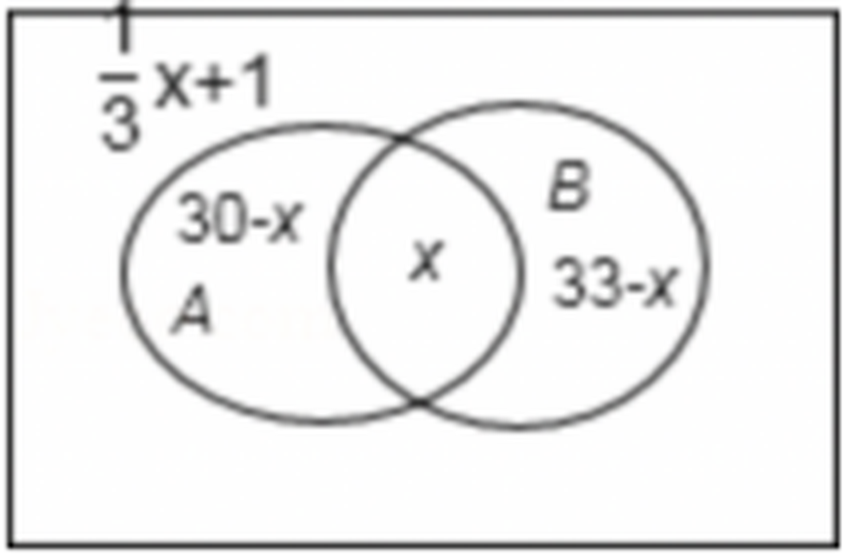
\includegraphics[width=0.30\textwidth]{figures/venn_AB_survey_50.png}
\end{center}

\ans{$21$}

\ifanswer
\solbegin
\step{由题意得赞成 $A$ 的人数 30，赞成 $B$ 的人数为 33，}
\step{设对 $A$、$B$ 都赞成的学生数为 $x$，则对 $A$、$B$ 都不赞成的学生数 $\dfrac{1}{3}x+1$，}
\step{如图得 $x+30-x+33-x+\dfrac{1}{3}x+1=50$，所以 $x=21$.}
\solend

\fi

\item 集合 $S=\{s\mid s=2n+1,n\in\Z\}$，$T=\{t\mid t=4n+1,n\in\Z\}$，则 $S$ \blankline[2.4em] $T$（填“$\subset$”“$\supset$”“$\subseteq$”或“$\supseteq$”）.

\ans{$S\supset T$}

\ifanswer
\solbegin
\step{对于 $S=\{s\mid s=2n+1,n\in\Z\}$ 为奇数，}
\step{而 $T=\{t\mid t=4n+1,n\in\Z\}$ 被 4 整除余 1 的奇数，所以 $S\supset T$.}
\solend

\fi

\item 已知集合 $A=\{x\mid -2<x<4\}$，$B=\{x\mid x^2-3ax+2a^2=0\}$，若 $A\cap B=B$，则实数 $a$ 的取值范围为 \blankline[4.4em].

\ans{$(-1,2)$}

\ifanswer
\solbegin
\step{因为 $A\cap B=B$，所以 $B\subseteq A$，}
\step{①当 $a=0$ 时，方程 $x^2-3ax+2a^2=0$ 的解为 $0$，$B\subseteq A$ 成立；}
\step{②当 $a\neq 0$ 时，方程 $x^2-3ax+2a^2=0$ 的解为 $2a$、$a$，}
\step{则 $-2<2a<4$ 且 $-2<a<4$，解得 $-1<a<2$ 且 $a\neq 0$；}
\step{综上所述，实数 $a$ 的取值范围为 $(-1,2)$.}
\solend

\fi

\item 当一个非空数集 $F$ 满足条件“若 $a$、$b\in F$，则 $a+b$、$a-b$、$ab\in F$，且当 $b\neq 0$ 时，$\dfrac{a}{b}\in F$”时，称 $F$ 为一个数域，以下四个关于数域的命题：

（1）$0$ 是任何数域的元素；（2）若数域 $F$ 有非零元素，则 $2026\in F$；

（3）集合 $P=\{x\mid x=3k,k\in\Z\}$ 为数域；（4）有理数集为数域；

其中，真命题的编号为 \blankline[4.4em]（写出所有真命题的编号）.

\ans{（1）（2）（4）}

\item 对于集合 $M$，定义函数 $f_M(x)=\begin{cases}-1,&x\in M\\ 1,&x\notin M\end{cases}$，对于两个集合 $M$、$N$，定义集合
$M\triangle N=\{x\mid f_M(x)\cdot f_N(x)=-1\}$，已知 $A=\{2,4,6,8,10\},B=\{1,2,4,8,16\}$，用 $|M|$ 表示有限集合 $M$ 中的元素个数，则对于任意集合 $M$，$|M\triangle A|+|M\triangle B|$ 的最小值为 \blankline[2.4em].

% 注：上面分段函数的第二行，原卷印作「1, $x\in M$」（两行都印 $x\in M$），与函数的定义矛盾，
%     本稿按文意订正为 $x\notin M$.
\ans{$4$}

\ifanswer
\solbegin
% 注：下面一行原卷印作「即 $M\triangle N\in\{x\mid x\in M\cup N\}$ 且 $x\in M\cap N$」，「$\in$」当为
%     「$=$」之误，且由 $f_M(x)f_N(x)=-1$ 应对应 $x\notin M\cap N$，本稿一并按文意订正.
\step{由 $M\triangle N$ 的定义得 $f_M(x)\cdot f_N(x)=-1$，}
\step{即 $M\triangle N=\{x\mid x\in M\cup N\text{ 且 }x\notin M\cap N\}$，}
\step{$|M\triangle A|+|M\triangle B|$ 要取得最小值，需满足 $A\cap B\subseteq M\subseteq A\cup B$，}
\step{此时 $|M\triangle A|+|M\triangle B|$ 的最小值为 $4$.}
\solend

\fi

\end{enumerate}

\bigsec{二、选择题}

\begin{enumerate}
\setcounter{enumi}{12}

\item 已知集合 $A=\{x\mid x=3m,m\in\N\}$，$B=\{x\mid x=3m+1,m\in\N\}$，$C=\{x\mid x=3m+2,m\in\N\}$，若 $a\in A$，$b\in B$，$c\in C$，则下列结论中可能成立的是\mbox{（\quad）}

\keepwithprev
A. $2021=a+b+c$\qquad B. $2021=abc$\qquad C. $2021=a+bc$\qquad D. $2021=a(b+c)$

\ans{C}

\ifanswer
\solbegin
\step{由题意设 $a=3m$，$b=3p+1$，$c=3n+2$，$m$、$p$、$n\in\N$，}
\step{则 $a+b+c=3m+3p+1+3n+2=3(m+p+n+1)$，}
\step{故 2021 不是 3 的整数倍，则 A 不可能；}
\step{$abc=3m(3p+1)(3n+2)$，同理 B 不可能；}
\step{$a+bc=3m+(3p+1)(3n+2)=3(m+3pn+2p+n)+2$，$2021=3\times 673+2$，}
\step{如取 $p=n=1$，则 $m=667$，即 $2021=3\times 667+4\times 5$，故 C 成立；}
\step{$a(b+c)=3m(3p+1+3n+2)=9m(p+n+1)$，同 A 可得 D 不可能.}
\step{故选 C.}
\solend

\fi

\item 设 $a$、$b$、$c$ 是实数，$x=a^2-2b+\dfrac{\pi}{3}$，$y=b^2-2c+\dfrac{\pi}{6}$，$z=c^2-2a+\dfrac{\pi}{2}$，则 $x$、$y$、$z$ 中至少有一个值\mbox{（\quad）}

\keepwithprev
A. 大于 $0$\qquad B. 等于 $0$\qquad C. 不大于 $0$\qquad D. 小于 $0$

\ans{A}

\ifanswer
\solbegin
\step{因为 $x+y+z=a^2-2b+\dfrac{\pi}{3}+b^2-2c+\dfrac{\pi}{6}+c^2-2a+\dfrac{\pi}{2}=(a-1)^2+(b-1)^2+(c-1)^2+\pi-3>0$，}
\step{假设 $x$、$y$、$z$ 都不大于 $0$，即 $x\leqslant 0$，$y\leqslant 0$，$z\leqslant 0$，}
\step{由同向不等式的可加性得 $x+y+z\leqslant 0$①，又 $x+y+z>0$ 与①式矛盾.}
\step{所以假设不成立，即原命题的结论 $x$、$y$、$z$ 中至少有一个大于 $0$. 故选 A.}
\solend

\fi

\item 命题“存在一个无理数，它的平方是有理数”的否定是\mbox{（\quad）}

\keepwithprev
A. 任意一个有理数，它的平方是有理数

B. 任意一个无理数，它的平方不是有理数

C. 存在一个有理数，它的平方是有理数

D. 存在一个无理数，它的平方不是有理数

\ans{B}

\ifanswer
\solbegin
\step{否定是任意一个无理数，它的平方不是有理数，故选 B.}
\solend

\fi

\item 设集合 $P_1=\{x\mid x^2+ax+1>0\}$，$P_2=\{x\mid x^2+ax+2>0\}$，$Q_1=\{x\mid x^2+x+b>0\}$，$Q_2=\{x\mid x^2+2x+b>0\}$，其中 $a$、$b\in\R$，下列说法正确的是\mbox{（\quad）}

\keepwithprev
A. 对任意 $a$，$P_1$ 是 $P_2$ 的子集，对任意 $b$，$Q_1$ 不是 $Q_2$ 的子集

B. 对任意 $a$，$P_1$ 是 $P_2$ 的子集，存在 $b$，使得 $Q_1$ 是 $Q_2$ 的子集

C. 对任意 $a$，使得 $P_1$ 不是 $P_2$ 的子集，对任意 $b$，$Q_1$ 不是 $Q_2$ 的子集

D. 对任意 $a$，使得 $P_1$ 不是 $P_2$ 的子集，存在 $b$，使得 $Q_1$ 不是 $Q_2$ 的子集

\ans{B}

\ifanswer
\solbegin
\step{对于集合 $P_1=\{x\mid x^2+ax+1>0\}$，$P_2=\{x\mid x^2+ax+2>0\}$，}
\step{得当 $m\in P_1$，即 $m^2+am+1>0$，得 $m^2+am+2>0$，}
\step{即有 $m\in P_2$，得对任意 $a$，$P_1$ 是 $P_2$ 的子集；}
\step{当 $b=5$ 时，$Q_1=\{x\mid x^2+x+5>0\}=\R$，$Q_2=\{x\mid x^2+2x+5>0\}=\R$，}
\step{得 $Q_1$ 是 $Q_2$ 的子集，故 A 错误，B 正确；}
\step{当 $b=1$ 时，$Q_1=\{x\mid x^2+x+1>0\}=\R$，}
\step{$Q_2=\{x\mid x^2+2x+1>0\}=\{x\mid x\neq -1\text{ 且 }x\in\R\}$，得 $Q_1$ 不是 $Q_2$ 的子集.}
\step{综上，对任意 $a$，$P_1$ 是 $P_2$ 的子集，存在 $b$，使得 $Q_1$ 是 $Q_2$ 的子集，}
\step{故 C 错误，D 错误.}
\step{故选 B.}
\solend

\fi

\end{enumerate}

\bigsec{三、解答题}

\begin{enumerate}
\setcounter{enumi}{16}

\item 已知集合 $A=\{x\mid 0<x-a\leqslant 5\}$，$B=\left\{x\mid -\dfrac{a}{2}<x\leqslant 6\right\}$.

\begin{enumerate}[label=(\arabic*)]
\item 若 $A\subseteq B$，求 $a$ 的取值范围.
\item 集合 $A$ 与 $B$ 能否相等？若能，求出 $a$ 的值，若不能，请说明理由.
\end{enumerate}

\ans{（1）$0\leqslant a\leqslant 1$；（2）不能，$a\in\varnothing$}

\ifanswer
\solbegin
\stepm{（1）}{由于 $A\subseteq B$，所以 $a+5\leqslant 6$，且 $-\dfrac{a}{2}\leqslant a$，解得 $0\leqslant a\leqslant 1$；}
\stepm{（2）}{$A=B$ 时，$a+5=6$，$-\dfrac{a}{2}=a$，解得 $a\in\varnothing$.}
\solend

\fi

\ansspace[6]

\item 已知 $\alpha:2x+m<0$，$\beta:-1<x<3$.

\begin{enumerate}[label=(\arabic*)]
\item 是否存在实数 $m$，使得 $\alpha$ 是 $\beta$ 的充分条件？若存在，求出实数 $m$ 的取值范围；
\item 是否存在实数 $m$，使得 $\alpha$ 是 $\beta$ 的必要条件？若存在，求出实数 $m$ 的取值范围.
\end{enumerate}

\ans{（1）不存在；（2）存在，$m\leqslant -6$}

\ansspace[6]

\item 已知 $\triangle ABC$ 的三边长分别为 $a,b,c$，证明：

\begin{enumerate}[label=(\arabic*)]
\item “$A=90^\circ$”是“关于 $x$ 的方程 $x^2+2ax+b^2=0$ 与 $x^2+2cx-b^2=0$ 有公共实根”的充分条件；
\item “$a=c$”是“关于 $x$ 的方程 $x^2+2ax+b^2=0$ 与 $x^2+2cx-b^2=0$ 没有公共实根”的充分非必要条件.
\end{enumerate}

\ans{（1）略；（2）略}

\ansspace[8]

\item 已知集合 $A$ 包含有 $n(n\in\N^*)$ 个元素，$A^+=\{x+y\mid x\text{、}y\in A\}$.

\begin{enumerate}[label=(\arabic*)]
\item 若 $A=\{0,1,2\}$，写出 $A^+$；
\item % 注：原卷此处印作「写出一个 $A^+$，使得 $A=A^+$」——$A$ 未给定，该问无法作答，
      %     与下方【解析】「取 $A=\{0\}$」不符，本稿按文意订正为「写出一个 $A$」.
      写出一个 $A$，使得 $A=A^+$；
\item 当 $n=4$ 时，是否存在集合 $A$，使得 $A^+=\{2,3,5,6,7,8,10\}$？若存在，求出此时的集合 $A$，若不存在，请说明理由.
\end{enumerate}

\ans{（1）$\{0,1,2,3,4\}$；（2）$A=\{0\}$；（3）不存在}

\ifanswer
\solbegin
\stepm{（1）}{由题意得 $0+0=0$，$0+1=1$，$0+2=2$，$1+1=2$，$1+2=3$，$2+2=4$ 都是 $A^+$ 中的元素，故 $A^+=\{0,1,2,3,4\}$；}
\stepm{（2）}{取 $A=\{0\}$，此时 $A^+=\{x+y\mid x\text{、}y\in A\}=\{0\}$，符合 $A=A^+$；}
\stepm{（3）}{当 $n=4$ 时，不存在集合 $A$，使得 $A^+=\{2,3,5,6,7,8,10\}$，理由如下：}
\step{假设存在 $A=\{a,b,c,d\}$，且 $a<b<c<d$，}
\step{则 $2a<a+b<a+c<b+c<b+d<c+d<2d$，}
\step{故 $2a,a+b,a+c,b+c,b+d,c+d,2d$ 为 $A^+$ 中 7 个不同的元素，}
\step{则 $2a=2$，$a+b=3$，$a+c=5$，$b+c=6$，$b+d=7$，$c+d=8$，$2d=10$，}
\step{解得 $a=1$，$b=2$，$c=4$，$d=5$，}
\step{此时 $c+d=9\in A^+$ 与 $9\notin A^+$ 矛盾，故假设不成立，}
\step{即不存在这样的集合 $A$.}
\solend

\fi

\ansspace[8]

% 压轴题：在其 \item 前先量一下版面，本页剩余高度不足 7cm 就另起一页。
\ansneed{7cm}

\item 已知集合 $A$ 为非空数集，对于集合 $A$，对 $A$ 中任意两个不同元素相加得到的和取绝对值，将这些绝对值重新组成一个新的集合，对于这一过程，我们定义为“自相加”，重新组成的集合叫做“集合 $A$ 的 1 次自相加集合”，再进行 $n-1$ 次“自相加”操作，组成的集合叫做“集合 $A$ 的 $n$ 次自相加集合”. 若集合 $A$ 的任意 $k$ 次自相加集合都不相等，则称集合 $A$ 为“完美自相加集合”，同理，我们可以定义出“$A$ 的 1 次自相减集合”，集合 $A$ 的 1 次自相加集合和 1 次自相减集合分别可表示为：$A^+=\{x\mid x=|a+b|,\ a\text{、}b\in A\}$，$A^-=\{x\mid x=|a-b|,\ a\text{、}b\in A\}$.

\begin{enumerate}[label=(\arabic*)]
\item 已知有两个集合，集合 $B=\{1,2,3,4\}$，集合 $C=\{k\mid k=2n+1,n\in\Z\}$，判断集合 $B$ 和集合 $C$ 是否是完美自相加集合，并说明理由；
\item 对（1）中的集合 $B$ 进行 11 次自相加操作后，求：集合 $B$ 的 11 次自相加集合的元素个数；
\item 若 $0\leqslant n\leqslant 2025$ 且 $n\in\N$，集合 $A=\{x\mid n\leqslant x\leqslant 2025,x\in\N\}$，$A^+\cap A^-=\varnothing$，求：$n$ 的最小值.
\end{enumerate}

\ans{（1）$B$ 是完美自相加集合，$C$ 不是完美自相加集合；（2）$2051$；（3）$675$}

\ifanswer
\solbegin
\stepm{（1）}{$B$ 是完美自相加集合，$C$ 不是完美自相加集合，}
\step{理由如下：因为集合 $B=\{1,2,3,4\}$，所以 $B^+=\{3,4,5,6,7\}$，}
\step{由此可得集合自相加后，}
\step{新的集合中最小的元素为自相加之前的集合中的最小两个元素之和，}
\step{所以显然集合 $B=\{1,2,3,4\}$ 的最小两个元素为 $1$，$2$，}
\step{所以 $B^+$ 中的最小元素为 $1+2=3$，}
\step{同理，2 次自相加后得到的集合中的最小元素是 $3+4=7$.}
\step{依照这样的规律，对集合 $B=\{1,2,3,4\}$ 进行任意次自相加操作后，}
\step{最小值总在变大，故不可能有相等集合，所以 $B$ 是完美自相加集合；}
\step{因为集合 $C=\{k\mid k=2n+1,n\in\Z\}$ 表示所有奇数构成的集合，}
\step{任何两个奇数相加的和都是偶数，}
\step{所以 $C^+=\{k\mid k=2n,n\in\Z\}$ 为所有偶数构成集合；}
\step{所以对 $C^+=\{k\mid k=2n,n\in\Z\}$ 再进行一次自相加操作，}
\step{因为任意两个偶数相加的和还是偶数，}
\step{所以后面集合不管进行多少次相加都与 $C^+=\{k\mid k=2n,n\in\Z\}$ 相同；}
\step{故 $C$ 不是完美自相加集合.}
\stepm{（2）}{由自相加性质得，对于集合 $B=\{1,2,3,4\}$，进行一次自相加，}
\step{得到集合的最小值必然是原来集合的两个最小元素值之和，}
\step{得到的最大值必然为原来集合的两个最大元素值之和，}
\step{且中间必然是连续的整数元素；}
\step{所以对集合 $B=\{1,2,3,4\}$ 进行 1 次自相加之后，}
\step{得到的集合最小两个元素为 $3$，$4$，最大的两个元素为 $6$，$7$；}
\step{进行第 2 次自相加，得到的集合最小两个元素为 $7$，$8$，}
\step{最大的两个元素为 $12$，$13$；}
\step{进行第 3 次自相加，得到的集合最小两个元素为 $15$，$16$，}
\step{最大的两个元素为 $24$，$25$；}
\step{进行第 4 次自相加，得到的集合最小两个元素为 $31$，$32$，}
\step{最大的两个元素为 $48$，$49$；}
\step{进行第 5 次自相加，得到的集合最小两个元素为 $63$，$64$，}
\step{最大的两个元素为 $96$，$97$；}
\step{进行第 6 次自相加，得到的集合最小两个元素为 $127$，$128$，}
\step{最大的两个元素为 $192$，$193$；}
\step{进行第 7 次自相加，得到的集合最小两个元素为 $255$，$256$，}
\step{最大的两个元素为 $384$，$385$；}
\step{进行第 8 次自相加，得到的集合最小两个元素为 $511$，$512$，}
\step{最大的两个元素为 $768$，$769$；}
\step{进行第 9 次自相加，得到的集合最小两个元素为 $1023$，$1024$，}
\step{最大的两个元素为 $1536$，$1537$；}
\step{进行第 10 次自相加，得到的集合最小两个元素为 $2047$，$2048$，}
\step{最大的两个元素为 $3072$，$3073$；}
\step{进行第 11 次自相加，得到的集合最小两个元素为 $4095$，$4096$，}
\step{最大的两个元素为 $6144$，$6145$；}
\step{因为集合 $B$ 的 $n$ 次自相加集合中的元素都是连续的整数，}
\step{所以集合 $B$ 进行 11 次自相加操作后的元素个数为 $6145-4095+1=2051$.}
\stepm{（3）}{因为 $0\leqslant n\leqslant 2025$ 且 $n\in\N$，集合 $A=\{x\mid n\leqslant x\leqslant 2025,x\in\N\}$，}
\step{所以 $A^+=\{x\mid 2n+1\leqslant x\leqslant 4049,x\in\N\}$，}
\step{$A^-=\{x\mid 1\leqslant x\leqslant 2025-n,x\in\N\}$，}
\step{要使 $A^+\cap A^-=\varnothing$，须使 $2n+1>2025-n$，所以 $n>\dfrac{2024}{3}=674\dfrac{2}{3}$，}
\step{又 $n\in\N$，故 $n$ 的最小值为 $675$.}
\solend

\fi

% 压轴题：其后已无内容，故作答区全用可丢弃胶水（\ansspace*）。
\ansspace*[12]

\end{enumerate}

\end{document}
"
% 紧凑版：xelatex "\def\iscompact{1}% 高一17_七宝中学_周末作业2.tex —— 高一上数学「2026-2027 年七宝中学高一上周末作业 2」（试卷版/答案版）
% 试卷版：xelatex 高一17_七宝中学_周末作业2.tex
% 答案版：xelatex "\def\isanswer{1}\input{高一17_七宝中学_周末作业2.tex}"
% 紧凑版：xelatex "\def\iscompact{1}\input{高一17_七宝中学_周末作业2.tex}"
%
% 原始材料是微信公众号图文（公众号「魔都数学加油站」），正文为 10 张 PNG 页（1080×1527）。
% 原文本身就是一份**讲评版**——题目下方直接印出【答案】或【解析】，选择题的答案印在解析末句
% 「故选 X」里。试题文字、答案与解析均照原卷录入（订正处见下），卷面上的粉色斜水印
% 「魔都数学加油站」属水印，未录入。
%
% 与原卷的排版差异（均已在 README「说明」中交代）：
%   ① 原文自**第 3 题**起（第 1、2 题未在该文中发布），故本稿题号亦自 3 起；
%   ② 原卷本就印有「一、填空题」「二、选择题」「三、解答题」三节标题（分别在原图 00/02/04.png
%      上，逐页核对过），本稿照原卷分节，只把标题改排成全稿统一的「大节标题」样式；
%   ③ 原卷填空、选择的答案直接印在题目下方（选择题只在解析末句「故选 X」中给出），本稿统一改为
%      试卷版隐去、答案版以【答案】给出，选择题的括注一律改排「\mbox{（\quad）}」并把答案移到选项之后，
%      使两版彻底分离；
%   ④ 原卷的集合符号大小写混用：第 3 题题干的实数集印成**粗体** $\mathbf{R}$，第 16 题题干与
%      第 16 题解析的印成正体 $R$；自然数集 $N$、整数集 $Z$ 一律正体。本稿按全稿惯例统一写作
%      $\R$、$\N$、$\Z$；
%   ⑤ 原卷未印副标题，本稿按全稿惯例补出副标题「集合与常用逻辑用语」；
%   ⑥ 原卷解答题子问编号为「（1）（2）」，本稿用嵌套 enumerate 排成同一形态；原卷第 15 题的
%      D 选项因原页翻页被截到下一页首页，本稿自然连排；
%   ⑦ 原卷解答题未留作答空间（讲评稿通篇是答案），本稿逐题补出书写留白，仅试卷版显示；
%   ⑧ 第 21 题题干里 $A^+$、$A^-$ 的定义含绝对值号（原卷作 $\{x\mid x=|a+b|,\ a\text{、}b\in A\}$
%      与 $\{x\mid x=|a-b|,\ a\text{、}b\in A\}$），本稿照原卷录入；2026-09-15 回原图逐处放大复核
%      时发现曾漏抄两处绝对值号、并把分隔逗号误写成 $\mid$，已按原卷订正（见 README 专记）。
%
% 原卷笔误三处（均已放大到能看清字形后核对，本稿按文意订正，并在 README 中写明原委）：
%   ① 第 12 题题干的分段函数 $f_M(x)$ 原卷两行都印作「$x\in M$」（$-1$ 与 $1$ 都取在 $M$ 上），
%      与「函数」的定义直接矛盾（$M$ 上无法同时取两个值），按文意订正第二行为 $x\notin M$；
%   ② 第 12 题【解析】首行原卷印「即 $M\triangle N\in\{x\mid x\in M\cup N\}$ 且 $x\in M\cap N$」，
%      其中「$\in$」当为「$=$」之误；且由 $f_M(x)f_N(x)=-1$ 应对应 $x\notin M\cap N$（原卷印作
%      $x\in M\cap N$，与上一行刚写出的对称差的定义相矛盾），本稿一并订正；
%   ③ 第 20 题(2)原卷印「写出一个 $A^+$，使得 $A=A^+$」——$A$ 未给定，该问无法作答，与紧接的
%      【解析】「取 $A=\{0\}$，此时 $A^+=\{0\}$，符合 $A=A^+$」不符，本稿按文意订正为
%      「写出一个 $A$，使得 $A=A^+$」.
%
% 原卷存疑一处（无法确证原意，本稿照抄原卷、未改）：
%   ① 第 5 题 ④ 原卷题干印 $S=\{x\mid |x|\leqslant\sqrt{3},x\in N\}$（该字母与 ③ 中的 $Z$
%      字形明显不同，$Z$ 有上下两横，已放大比对确认），而【解析】印「因为 $S=\{-1,0,1\}$」——
%      按 $x\in N$ 应为 $S=\{0,1\}$（或 $\{1\}$），题干与解析的口径不一致；但无论取哪一口径，
%      ④ 都是 $M$ 的子集、本题结论（填④）不变，故题干与解析均照抄原卷，未改。

\documentclass[a4paper,11pt]{article}
\usepackage{common}

\begin{document}

\examtitlest{2026--2027 年七宝中学高一上周末作业 2}{集合与常用逻辑用语}

\bigsec{一、填空题}

\begin{enumerate}
\setcounter{enumi}{2}

\item 已知 $a,x\in\R$，则“$x\in\{-a,a\}$”是“$|x|=a$”的 \blankline[4.4em] 条件.

\ans{必要不充分}

\item 设全集为 $U$，$A\subseteq U$，$B\subseteq U$，则“$A\subset B$”是“$\overline{B}\subset\overline{A}$”的 \blankline[4.4em] 条件.

\ans{充要}

\item 已知集合 $M=\{x\mid -\sqrt{5}<x<\sqrt{3},x\in\Z\}$，则下列集合是集合 $M$ 的子集的是 \blankline[4.4em]（填序号）.

① $P=\{-3,0,1\}$；② $Q=\{-1,0,1,2\}$；③ $R=\{y\mid -\pi<y<-1,y\in\Z\}$；

④ $S=\{x\mid |x|\leqslant\sqrt{3},x\in\N\}$.

\ans{④}

\ifanswer
\solbegin
\step{由已知得集合 $M=\{-2,-1,0,1\}$，}
\step{所以由子集的定义得选项①错误，②错误，}
\step{因为 $R=\{-3,-2\}$，所以集合 $R$ 不表示集合 $M$ 的子集，③错误，}
\step{因为 $S=\{-1,0,1\}$，所以是集合 $M$ 的子集，故正确.}
\step{故是集合 $M$ 的子集的是④.}
\solend

\fi

\item 已知 $x\in\R$，用反证法证明命题“若 $x^2-7x+10<0$，则 $2<x<5$”时，应该假设 \blankline[5em].

\ans{$x\leqslant 2$ 或 $x\geqslant 5$}

\item 设 $a_1,b_1,c_1,a_2,b_2,c_2$ 均为非零实数，方程 $a_1x^2+b_1x+c_1=0$ 和 $a_2x^2+b_2x+c_2=0$ 的解集分别为 $M$ 和 $N$，那么“$\dfrac{a_1}{a_2}=\dfrac{b_1}{b_2}=\dfrac{c_1}{c_2}$”是“$M=N$”的 \blankline[4.4em] 条件.

（填“充分非必要”、“必要非充分”、“充要”、或“既非充分又非必要”）

\ans{充分非必要}

\ifanswer
\solbegin
\step{$\dfrac{a_1}{a_2}=\dfrac{b_1}{b_2}=\dfrac{c_1}{c_2}$ 能推出 $M=N$，}
\step{若 $M=N=\varnothing$ 推不出 $\dfrac{a_1}{a_2}=\dfrac{b_1}{b_2}=\dfrac{c_1}{c_2}$，}
\step{所以“$\dfrac{a_1}{a_2}=\dfrac{b_1}{b_2}=\dfrac{c_1}{c_2}$”是“$M=N$”的“充分非必要”条件.}
\solend

\fi

\item 向 50 名学生调查对 $A$、$B$ 两事件的态度，有如下结果赞成 $A$ 的人数是全体的五分之三，其余的不赞成，赞成 $B$ 的比赞成 $A$ 的多 3 人，其余的不赞成；另外，对 $A$、$B$ 都不赞成的学生数比对 $A$、$B$ 都赞成的学生数的三分之一多 1 人. 则对 $A$、$B$ 都赞成的学生有 \blankline[2.4em] 人.

\begin{center}
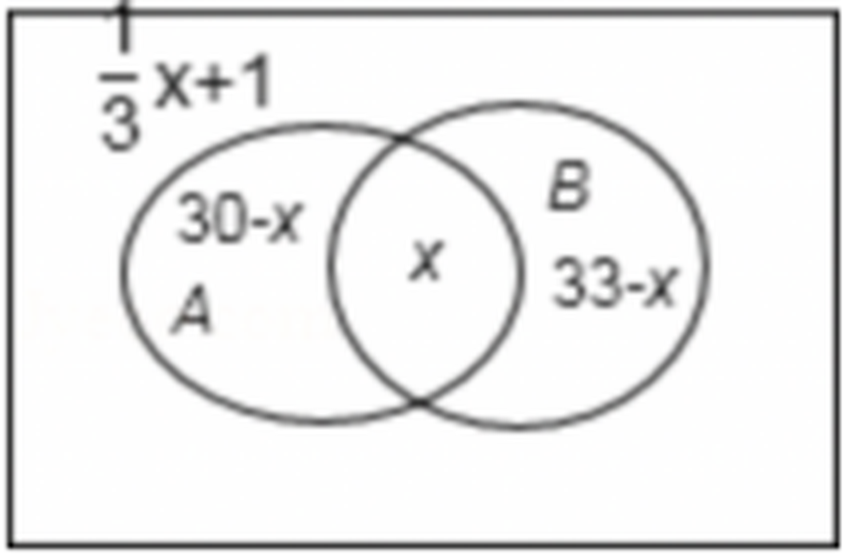
\includegraphics[width=0.30\textwidth]{figures/venn_AB_survey_50.png}
\end{center}

\ans{$21$}

\ifanswer
\solbegin
\step{由题意得赞成 $A$ 的人数 30，赞成 $B$ 的人数为 33，}
\step{设对 $A$、$B$ 都赞成的学生数为 $x$，则对 $A$、$B$ 都不赞成的学生数 $\dfrac{1}{3}x+1$，}
\step{如图得 $x+30-x+33-x+\dfrac{1}{3}x+1=50$，所以 $x=21$.}
\solend

\fi

\item 集合 $S=\{s\mid s=2n+1,n\in\Z\}$，$T=\{t\mid t=4n+1,n\in\Z\}$，则 $S$ \blankline[2.4em] $T$（填“$\subset$”“$\supset$”“$\subseteq$”或“$\supseteq$”）.

\ans{$S\supset T$}

\ifanswer
\solbegin
\step{对于 $S=\{s\mid s=2n+1,n\in\Z\}$ 为奇数，}
\step{而 $T=\{t\mid t=4n+1,n\in\Z\}$ 被 4 整除余 1 的奇数，所以 $S\supset T$.}
\solend

\fi

\item 已知集合 $A=\{x\mid -2<x<4\}$，$B=\{x\mid x^2-3ax+2a^2=0\}$，若 $A\cap B=B$，则实数 $a$ 的取值范围为 \blankline[4.4em].

\ans{$(-1,2)$}

\ifanswer
\solbegin
\step{因为 $A\cap B=B$，所以 $B\subseteq A$，}
\step{①当 $a=0$ 时，方程 $x^2-3ax+2a^2=0$ 的解为 $0$，$B\subseteq A$ 成立；}
\step{②当 $a\neq 0$ 时，方程 $x^2-3ax+2a^2=0$ 的解为 $2a$、$a$，}
\step{则 $-2<2a<4$ 且 $-2<a<4$，解得 $-1<a<2$ 且 $a\neq 0$；}
\step{综上所述，实数 $a$ 的取值范围为 $(-1,2)$.}
\solend

\fi

\item 当一个非空数集 $F$ 满足条件“若 $a$、$b\in F$，则 $a+b$、$a-b$、$ab\in F$，且当 $b\neq 0$ 时，$\dfrac{a}{b}\in F$”时，称 $F$ 为一个数域，以下四个关于数域的命题：

（1）$0$ 是任何数域的元素；（2）若数域 $F$ 有非零元素，则 $2026\in F$；

（3）集合 $P=\{x\mid x=3k,k\in\Z\}$ 为数域；（4）有理数集为数域；

其中，真命题的编号为 \blankline[4.4em]（写出所有真命题的编号）.

\ans{（1）（2）（4）}

\item 对于集合 $M$，定义函数 $f_M(x)=\begin{cases}-1,&x\in M\\ 1,&x\notin M\end{cases}$，对于两个集合 $M$、$N$，定义集合
$M\triangle N=\{x\mid f_M(x)\cdot f_N(x)=-1\}$，已知 $A=\{2,4,6,8,10\},B=\{1,2,4,8,16\}$，用 $|M|$ 表示有限集合 $M$ 中的元素个数，则对于任意集合 $M$，$|M\triangle A|+|M\triangle B|$ 的最小值为 \blankline[2.4em].

% 注：上面分段函数的第二行，原卷印作「1, $x\in M$」（两行都印 $x\in M$），与函数的定义矛盾，
%     本稿按文意订正为 $x\notin M$.
\ans{$4$}

\ifanswer
\solbegin
% 注：下面一行原卷印作「即 $M\triangle N\in\{x\mid x\in M\cup N\}$ 且 $x\in M\cap N$」，「$\in$」当为
%     「$=$」之误，且由 $f_M(x)f_N(x)=-1$ 应对应 $x\notin M\cap N$，本稿一并按文意订正.
\step{由 $M\triangle N$ 的定义得 $f_M(x)\cdot f_N(x)=-1$，}
\step{即 $M\triangle N=\{x\mid x\in M\cup N\text{ 且 }x\notin M\cap N\}$，}
\step{$|M\triangle A|+|M\triangle B|$ 要取得最小值，需满足 $A\cap B\subseteq M\subseteq A\cup B$，}
\step{此时 $|M\triangle A|+|M\triangle B|$ 的最小值为 $4$.}
\solend

\fi

\end{enumerate}

\bigsec{二、选择题}

\begin{enumerate}
\setcounter{enumi}{12}

\item 已知集合 $A=\{x\mid x=3m,m\in\N\}$，$B=\{x\mid x=3m+1,m\in\N\}$，$C=\{x\mid x=3m+2,m\in\N\}$，若 $a\in A$，$b\in B$，$c\in C$，则下列结论中可能成立的是\mbox{（\quad）}

\keepwithprev
A. $2021=a+b+c$\qquad B. $2021=abc$\qquad C. $2021=a+bc$\qquad D. $2021=a(b+c)$

\ans{C}

\ifanswer
\solbegin
\step{由题意设 $a=3m$，$b=3p+1$，$c=3n+2$，$m$、$p$、$n\in\N$，}
\step{则 $a+b+c=3m+3p+1+3n+2=3(m+p+n+1)$，}
\step{故 2021 不是 3 的整数倍，则 A 不可能；}
\step{$abc=3m(3p+1)(3n+2)$，同理 B 不可能；}
\step{$a+bc=3m+(3p+1)(3n+2)=3(m+3pn+2p+n)+2$，$2021=3\times 673+2$，}
\step{如取 $p=n=1$，则 $m=667$，即 $2021=3\times 667+4\times 5$，故 C 成立；}
\step{$a(b+c)=3m(3p+1+3n+2)=9m(p+n+1)$，同 A 可得 D 不可能.}
\step{故选 C.}
\solend

\fi

\item 设 $a$、$b$、$c$ 是实数，$x=a^2-2b+\dfrac{\pi}{3}$，$y=b^2-2c+\dfrac{\pi}{6}$，$z=c^2-2a+\dfrac{\pi}{2}$，则 $x$、$y$、$z$ 中至少有一个值\mbox{（\quad）}

\keepwithprev
A. 大于 $0$\qquad B. 等于 $0$\qquad C. 不大于 $0$\qquad D. 小于 $0$

\ans{A}

\ifanswer
\solbegin
\step{因为 $x+y+z=a^2-2b+\dfrac{\pi}{3}+b^2-2c+\dfrac{\pi}{6}+c^2-2a+\dfrac{\pi}{2}=(a-1)^2+(b-1)^2+(c-1)^2+\pi-3>0$，}
\step{假设 $x$、$y$、$z$ 都不大于 $0$，即 $x\leqslant 0$，$y\leqslant 0$，$z\leqslant 0$，}
\step{由同向不等式的可加性得 $x+y+z\leqslant 0$①，又 $x+y+z>0$ 与①式矛盾.}
\step{所以假设不成立，即原命题的结论 $x$、$y$、$z$ 中至少有一个大于 $0$. 故选 A.}
\solend

\fi

\item 命题“存在一个无理数，它的平方是有理数”的否定是\mbox{（\quad）}

\keepwithprev
A. 任意一个有理数，它的平方是有理数

B. 任意一个无理数，它的平方不是有理数

C. 存在一个有理数，它的平方是有理数

D. 存在一个无理数，它的平方不是有理数

\ans{B}

\ifanswer
\solbegin
\step{否定是任意一个无理数，它的平方不是有理数，故选 B.}
\solend

\fi

\item 设集合 $P_1=\{x\mid x^2+ax+1>0\}$，$P_2=\{x\mid x^2+ax+2>0\}$，$Q_1=\{x\mid x^2+x+b>0\}$，$Q_2=\{x\mid x^2+2x+b>0\}$，其中 $a$、$b\in\R$，下列说法正确的是\mbox{（\quad）}

\keepwithprev
A. 对任意 $a$，$P_1$ 是 $P_2$ 的子集，对任意 $b$，$Q_1$ 不是 $Q_2$ 的子集

B. 对任意 $a$，$P_1$ 是 $P_2$ 的子集，存在 $b$，使得 $Q_1$ 是 $Q_2$ 的子集

C. 对任意 $a$，使得 $P_1$ 不是 $P_2$ 的子集，对任意 $b$，$Q_1$ 不是 $Q_2$ 的子集

D. 对任意 $a$，使得 $P_1$ 不是 $P_2$ 的子集，存在 $b$，使得 $Q_1$ 不是 $Q_2$ 的子集

\ans{B}

\ifanswer
\solbegin
\step{对于集合 $P_1=\{x\mid x^2+ax+1>0\}$，$P_2=\{x\mid x^2+ax+2>0\}$，}
\step{得当 $m\in P_1$，即 $m^2+am+1>0$，得 $m^2+am+2>0$，}
\step{即有 $m\in P_2$，得对任意 $a$，$P_1$ 是 $P_2$ 的子集；}
\step{当 $b=5$ 时，$Q_1=\{x\mid x^2+x+5>0\}=\R$，$Q_2=\{x\mid x^2+2x+5>0\}=\R$，}
\step{得 $Q_1$ 是 $Q_2$ 的子集，故 A 错误，B 正确；}
\step{当 $b=1$ 时，$Q_1=\{x\mid x^2+x+1>0\}=\R$，}
\step{$Q_2=\{x\mid x^2+2x+1>0\}=\{x\mid x\neq -1\text{ 且 }x\in\R\}$，得 $Q_1$ 不是 $Q_2$ 的子集.}
\step{综上，对任意 $a$，$P_1$ 是 $P_2$ 的子集，存在 $b$，使得 $Q_1$ 是 $Q_2$ 的子集，}
\step{故 C 错误，D 错误.}
\step{故选 B.}
\solend

\fi

\end{enumerate}

\bigsec{三、解答题}

\begin{enumerate}
\setcounter{enumi}{16}

\item 已知集合 $A=\{x\mid 0<x-a\leqslant 5\}$，$B=\left\{x\mid -\dfrac{a}{2}<x\leqslant 6\right\}$.

\begin{enumerate}[label=(\arabic*)]
\item 若 $A\subseteq B$，求 $a$ 的取值范围.
\item 集合 $A$ 与 $B$ 能否相等？若能，求出 $a$ 的值，若不能，请说明理由.
\end{enumerate}

\ans{（1）$0\leqslant a\leqslant 1$；（2）不能，$a\in\varnothing$}

\ifanswer
\solbegin
\stepm{（1）}{由于 $A\subseteq B$，所以 $a+5\leqslant 6$，且 $-\dfrac{a}{2}\leqslant a$，解得 $0\leqslant a\leqslant 1$；}
\stepm{（2）}{$A=B$ 时，$a+5=6$，$-\dfrac{a}{2}=a$，解得 $a\in\varnothing$.}
\solend

\fi

\ansspace[6]

\item 已知 $\alpha:2x+m<0$，$\beta:-1<x<3$.

\begin{enumerate}[label=(\arabic*)]
\item 是否存在实数 $m$，使得 $\alpha$ 是 $\beta$ 的充分条件？若存在，求出实数 $m$ 的取值范围；
\item 是否存在实数 $m$，使得 $\alpha$ 是 $\beta$ 的必要条件？若存在，求出实数 $m$ 的取值范围.
\end{enumerate}

\ans{（1）不存在；（2）存在，$m\leqslant -6$}

\ansspace[6]

\item 已知 $\triangle ABC$ 的三边长分别为 $a,b,c$，证明：

\begin{enumerate}[label=(\arabic*)]
\item “$A=90^\circ$”是“关于 $x$ 的方程 $x^2+2ax+b^2=0$ 与 $x^2+2cx-b^2=0$ 有公共实根”的充分条件；
\item “$a=c$”是“关于 $x$ 的方程 $x^2+2ax+b^2=0$ 与 $x^2+2cx-b^2=0$ 没有公共实根”的充分非必要条件.
\end{enumerate}

\ans{（1）略；（2）略}

\ansspace[8]

\item 已知集合 $A$ 包含有 $n(n\in\N^*)$ 个元素，$A^+=\{x+y\mid x\text{、}y\in A\}$.

\begin{enumerate}[label=(\arabic*)]
\item 若 $A=\{0,1,2\}$，写出 $A^+$；
\item % 注：原卷此处印作「写出一个 $A^+$，使得 $A=A^+$」——$A$ 未给定，该问无法作答，
      %     与下方【解析】「取 $A=\{0\}$」不符，本稿按文意订正为「写出一个 $A$」.
      写出一个 $A$，使得 $A=A^+$；
\item 当 $n=4$ 时，是否存在集合 $A$，使得 $A^+=\{2,3,5,6,7,8,10\}$？若存在，求出此时的集合 $A$，若不存在，请说明理由.
\end{enumerate}

\ans{（1）$\{0,1,2,3,4\}$；（2）$A=\{0\}$；（3）不存在}

\ifanswer
\solbegin
\stepm{（1）}{由题意得 $0+0=0$，$0+1=1$，$0+2=2$，$1+1=2$，$1+2=3$，$2+2=4$ 都是 $A^+$ 中的元素，故 $A^+=\{0,1,2,3,4\}$；}
\stepm{（2）}{取 $A=\{0\}$，此时 $A^+=\{x+y\mid x\text{、}y\in A\}=\{0\}$，符合 $A=A^+$；}
\stepm{（3）}{当 $n=4$ 时，不存在集合 $A$，使得 $A^+=\{2,3,5,6,7,8,10\}$，理由如下：}
\step{假设存在 $A=\{a,b,c,d\}$，且 $a<b<c<d$，}
\step{则 $2a<a+b<a+c<b+c<b+d<c+d<2d$，}
\step{故 $2a,a+b,a+c,b+c,b+d,c+d,2d$ 为 $A^+$ 中 7 个不同的元素，}
\step{则 $2a=2$，$a+b=3$，$a+c=5$，$b+c=6$，$b+d=7$，$c+d=8$，$2d=10$，}
\step{解得 $a=1$，$b=2$，$c=4$，$d=5$，}
\step{此时 $c+d=9\in A^+$ 与 $9\notin A^+$ 矛盾，故假设不成立，}
\step{即不存在这样的集合 $A$.}
\solend

\fi

\ansspace[8]

% 压轴题：在其 \item 前先量一下版面，本页剩余高度不足 7cm 就另起一页。
\ansneed{7cm}

\item 已知集合 $A$ 为非空数集，对于集合 $A$，对 $A$ 中任意两个不同元素相加得到的和取绝对值，将这些绝对值重新组成一个新的集合，对于这一过程，我们定义为“自相加”，重新组成的集合叫做“集合 $A$ 的 1 次自相加集合”，再进行 $n-1$ 次“自相加”操作，组成的集合叫做“集合 $A$ 的 $n$ 次自相加集合”. 若集合 $A$ 的任意 $k$ 次自相加集合都不相等，则称集合 $A$ 为“完美自相加集合”，同理，我们可以定义出“$A$ 的 1 次自相减集合”，集合 $A$ 的 1 次自相加集合和 1 次自相减集合分别可表示为：$A^+=\{x\mid x=|a+b|,\ a\text{、}b\in A\}$，$A^-=\{x\mid x=|a-b|,\ a\text{、}b\in A\}$.

\begin{enumerate}[label=(\arabic*)]
\item 已知有两个集合，集合 $B=\{1,2,3,4\}$，集合 $C=\{k\mid k=2n+1,n\in\Z\}$，判断集合 $B$ 和集合 $C$ 是否是完美自相加集合，并说明理由；
\item 对（1）中的集合 $B$ 进行 11 次自相加操作后，求：集合 $B$ 的 11 次自相加集合的元素个数；
\item 若 $0\leqslant n\leqslant 2025$ 且 $n\in\N$，集合 $A=\{x\mid n\leqslant x\leqslant 2025,x\in\N\}$，$A^+\cap A^-=\varnothing$，求：$n$ 的最小值.
\end{enumerate}

\ans{（1）$B$ 是完美自相加集合，$C$ 不是完美自相加集合；（2）$2051$；（3）$675$}

\ifanswer
\solbegin
\stepm{（1）}{$B$ 是完美自相加集合，$C$ 不是完美自相加集合，}
\step{理由如下：因为集合 $B=\{1,2,3,4\}$，所以 $B^+=\{3,4,5,6,7\}$，}
\step{由此可得集合自相加后，}
\step{新的集合中最小的元素为自相加之前的集合中的最小两个元素之和，}
\step{所以显然集合 $B=\{1,2,3,4\}$ 的最小两个元素为 $1$，$2$，}
\step{所以 $B^+$ 中的最小元素为 $1+2=3$，}
\step{同理，2 次自相加后得到的集合中的最小元素是 $3+4=7$.}
\step{依照这样的规律，对集合 $B=\{1,2,3,4\}$ 进行任意次自相加操作后，}
\step{最小值总在变大，故不可能有相等集合，所以 $B$ 是完美自相加集合；}
\step{因为集合 $C=\{k\mid k=2n+1,n\in\Z\}$ 表示所有奇数构成的集合，}
\step{任何两个奇数相加的和都是偶数，}
\step{所以 $C^+=\{k\mid k=2n,n\in\Z\}$ 为所有偶数构成集合；}
\step{所以对 $C^+=\{k\mid k=2n,n\in\Z\}$ 再进行一次自相加操作，}
\step{因为任意两个偶数相加的和还是偶数，}
\step{所以后面集合不管进行多少次相加都与 $C^+=\{k\mid k=2n,n\in\Z\}$ 相同；}
\step{故 $C$ 不是完美自相加集合.}
\stepm{（2）}{由自相加性质得，对于集合 $B=\{1,2,3,4\}$，进行一次自相加，}
\step{得到集合的最小值必然是原来集合的两个最小元素值之和，}
\step{得到的最大值必然为原来集合的两个最大元素值之和，}
\step{且中间必然是连续的整数元素；}
\step{所以对集合 $B=\{1,2,3,4\}$ 进行 1 次自相加之后，}
\step{得到的集合最小两个元素为 $3$，$4$，最大的两个元素为 $6$，$7$；}
\step{进行第 2 次自相加，得到的集合最小两个元素为 $7$，$8$，}
\step{最大的两个元素为 $12$，$13$；}
\step{进行第 3 次自相加，得到的集合最小两个元素为 $15$，$16$，}
\step{最大的两个元素为 $24$，$25$；}
\step{进行第 4 次自相加，得到的集合最小两个元素为 $31$，$32$，}
\step{最大的两个元素为 $48$，$49$；}
\step{进行第 5 次自相加，得到的集合最小两个元素为 $63$，$64$，}
\step{最大的两个元素为 $96$，$97$；}
\step{进行第 6 次自相加，得到的集合最小两个元素为 $127$，$128$，}
\step{最大的两个元素为 $192$，$193$；}
\step{进行第 7 次自相加，得到的集合最小两个元素为 $255$，$256$，}
\step{最大的两个元素为 $384$，$385$；}
\step{进行第 8 次自相加，得到的集合最小两个元素为 $511$，$512$，}
\step{最大的两个元素为 $768$，$769$；}
\step{进行第 9 次自相加，得到的集合最小两个元素为 $1023$，$1024$，}
\step{最大的两个元素为 $1536$，$1537$；}
\step{进行第 10 次自相加，得到的集合最小两个元素为 $2047$，$2048$，}
\step{最大的两个元素为 $3072$，$3073$；}
\step{进行第 11 次自相加，得到的集合最小两个元素为 $4095$，$4096$，}
\step{最大的两个元素为 $6144$，$6145$；}
\step{因为集合 $B$ 的 $n$ 次自相加集合中的元素都是连续的整数，}
\step{所以集合 $B$ 进行 11 次自相加操作后的元素个数为 $6145-4095+1=2051$.}
\stepm{（3）}{因为 $0\leqslant n\leqslant 2025$ 且 $n\in\N$，集合 $A=\{x\mid n\leqslant x\leqslant 2025,x\in\N\}$，}
\step{所以 $A^+=\{x\mid 2n+1\leqslant x\leqslant 4049,x\in\N\}$，}
\step{$A^-=\{x\mid 1\leqslant x\leqslant 2025-n,x\in\N\}$，}
\step{要使 $A^+\cap A^-=\varnothing$，须使 $2n+1>2025-n$，所以 $n>\dfrac{2024}{3}=674\dfrac{2}{3}$，}
\step{又 $n\in\N$，故 $n$ 的最小值为 $675$.}
\solend

\fi

% 压轴题：其后已无内容，故作答区全用可丢弃胶水（\ansspace*）。
\ansspace*[12]

\end{enumerate}

\end{document}
"
%
% 原始材料是微信公众号图文（公众号「魔都数学加油站」），正文为 10 张 PNG 页（1080×1527）。
% 原文本身就是一份**讲评版**——题目下方直接印出【答案】或【解析】，选择题的答案印在解析末句
% 「故选 X」里。试题文字、答案与解析均照原卷录入（订正处见下），卷面上的粉色斜水印
% 「魔都数学加油站」属水印，未录入。
%
% 与原卷的排版差异（均已在 README「说明」中交代）：
%   ① 原文自**第 3 题**起（第 1、2 题未在该文中发布），故本稿题号亦自 3 起；
%   ② 原卷本就印有「一、填空题」「二、选择题」「三、解答题」三节标题（分别在原图 00/02/04.png
%      上，逐页核对过），本稿照原卷分节，只把标题改排成全稿统一的「大节标题」样式；
%   ③ 原卷填空、选择的答案直接印在题目下方（选择题只在解析末句「故选 X」中给出），本稿统一改为
%      试卷版隐去、答案版以【答案】给出，选择题的括注一律改排「\mbox{（\quad）}」并把答案移到选项之后，
%      使两版彻底分离；
%   ④ 原卷的集合符号大小写混用：第 3 题题干的实数集印成**粗体** $\mathbf{R}$，第 16 题题干与
%      第 16 题解析的印成正体 $R$；自然数集 $N$、整数集 $Z$ 一律正体。本稿按全稿惯例统一写作
%      $\R$、$\N$、$\Z$；
%   ⑤ 原卷未印副标题，本稿按全稿惯例补出副标题「集合与常用逻辑用语」；
%   ⑥ 原卷解答题子问编号为「（1）（2）」，本稿用嵌套 enumerate 排成同一形态；原卷第 15 题的
%      D 选项因原页翻页被截到下一页首页，本稿自然连排；
%   ⑦ 原卷解答题未留作答空间（讲评稿通篇是答案），本稿逐题补出书写留白，仅试卷版显示；
%   ⑧ 第 21 题题干里 $A^+$、$A^-$ 的定义含绝对值号（原卷作 $\{x\mid x=|a+b|,\ a\text{、}b\in A\}$
%      与 $\{x\mid x=|a-b|,\ a\text{、}b\in A\}$），本稿照原卷录入；2026-09-15 回原图逐处放大复核
%      时发现曾漏抄两处绝对值号、并把分隔逗号误写成 $\mid$，已按原卷订正（见 README 专记）。
%
% 原卷笔误三处（均已放大到能看清字形后核对，本稿按文意订正，并在 README 中写明原委）：
%   ① 第 12 题题干的分段函数 $f_M(x)$ 原卷两行都印作「$x\in M$」（$-1$ 与 $1$ 都取在 $M$ 上），
%      与「函数」的定义直接矛盾（$M$ 上无法同时取两个值），按文意订正第二行为 $x\notin M$；
%   ② 第 12 题【解析】首行原卷印「即 $M\triangle N\in\{x\mid x\in M\cup N\}$ 且 $x\in M\cap N$」，
%      其中「$\in$」当为「$=$」之误；且由 $f_M(x)f_N(x)=-1$ 应对应 $x\notin M\cap N$（原卷印作
%      $x\in M\cap N$，与上一行刚写出的对称差的定义相矛盾），本稿一并订正；
%   ③ 第 20 题(2)原卷印「写出一个 $A^+$，使得 $A=A^+$」——$A$ 未给定，该问无法作答，与紧接的
%      【解析】「取 $A=\{0\}$，此时 $A^+=\{0\}$，符合 $A=A^+$」不符，本稿按文意订正为
%      「写出一个 $A$，使得 $A=A^+$」.
%
% 原卷存疑一处（无法确证原意，本稿照抄原卷、未改）：
%   ① 第 5 题 ④ 原卷题干印 $S=\{x\mid |x|\leqslant\sqrt{3},x\in N\}$（该字母与 ③ 中的 $Z$
%      字形明显不同，$Z$ 有上下两横，已放大比对确认），而【解析】印「因为 $S=\{-1,0,1\}$」——
%      按 $x\in N$ 应为 $S=\{0,1\}$（或 $\{1\}$），题干与解析的口径不一致；但无论取哪一口径，
%      ④ 都是 $M$ 的子集、本题结论（填④）不变，故题干与解析均照抄原卷，未改。

\documentclass[a4paper,11pt]{article}
\usepackage{common}

\begin{document}

\examtitlest{2026--2027 年七宝中学高一上周末作业 2}{集合与常用逻辑用语}

\bigsec{一、填空题}

\begin{enumerate}
\setcounter{enumi}{2}

\item 已知 $a,x\in\R$，则“$x\in\{-a,a\}$”是“$|x|=a$”的 \blankline[4.4em] 条件.

\ans{必要不充分}

\item 设全集为 $U$，$A\subseteq U$，$B\subseteq U$，则“$A\subset B$”是“$\overline{B}\subset\overline{A}$”的 \blankline[4.4em] 条件.

\ans{充要}

\item 已知集合 $M=\{x\mid -\sqrt{5}<x<\sqrt{3},x\in\Z\}$，则下列集合是集合 $M$ 的子集的是 \blankline[4.4em]（填序号）.

① $P=\{-3,0,1\}$；② $Q=\{-1,0,1,2\}$；③ $R=\{y\mid -\pi<y<-1,y\in\Z\}$；

④ $S=\{x\mid |x|\leqslant\sqrt{3},x\in\N\}$.

\ans{④}

\ifanswer
\solbegin
\step{由已知得集合 $M=\{-2,-1,0,1\}$，}
\step{所以由子集的定义得选项①错误，②错误，}
\step{因为 $R=\{-3,-2\}$，所以集合 $R$ 不表示集合 $M$ 的子集，③错误，}
\step{因为 $S=\{-1,0,1\}$，所以是集合 $M$ 的子集，故正确.}
\step{故是集合 $M$ 的子集的是④.}
\solend

\fi

\item 已知 $x\in\R$，用反证法证明命题“若 $x^2-7x+10<0$，则 $2<x<5$”时，应该假设 \blankline[5em].

\ans{$x\leqslant 2$ 或 $x\geqslant 5$}

\item 设 $a_1,b_1,c_1,a_2,b_2,c_2$ 均为非零实数，方程 $a_1x^2+b_1x+c_1=0$ 和 $a_2x^2+b_2x+c_2=0$ 的解集分别为 $M$ 和 $N$，那么“$\dfrac{a_1}{a_2}=\dfrac{b_1}{b_2}=\dfrac{c_1}{c_2}$”是“$M=N$”的 \blankline[4.4em] 条件.

（填“充分非必要”、“必要非充分”、“充要”、或“既非充分又非必要”）

\ans{充分非必要}

\ifanswer
\solbegin
\step{$\dfrac{a_1}{a_2}=\dfrac{b_1}{b_2}=\dfrac{c_1}{c_2}$ 能推出 $M=N$，}
\step{若 $M=N=\varnothing$ 推不出 $\dfrac{a_1}{a_2}=\dfrac{b_1}{b_2}=\dfrac{c_1}{c_2}$，}
\step{所以“$\dfrac{a_1}{a_2}=\dfrac{b_1}{b_2}=\dfrac{c_1}{c_2}$”是“$M=N$”的“充分非必要”条件.}
\solend

\fi

\item 向 50 名学生调查对 $A$、$B$ 两事件的态度，有如下结果赞成 $A$ 的人数是全体的五分之三，其余的不赞成，赞成 $B$ 的比赞成 $A$ 的多 3 人，其余的不赞成；另外，对 $A$、$B$ 都不赞成的学生数比对 $A$、$B$ 都赞成的学生数的三分之一多 1 人. 则对 $A$、$B$ 都赞成的学生有 \blankline[2.4em] 人.

\begin{center}
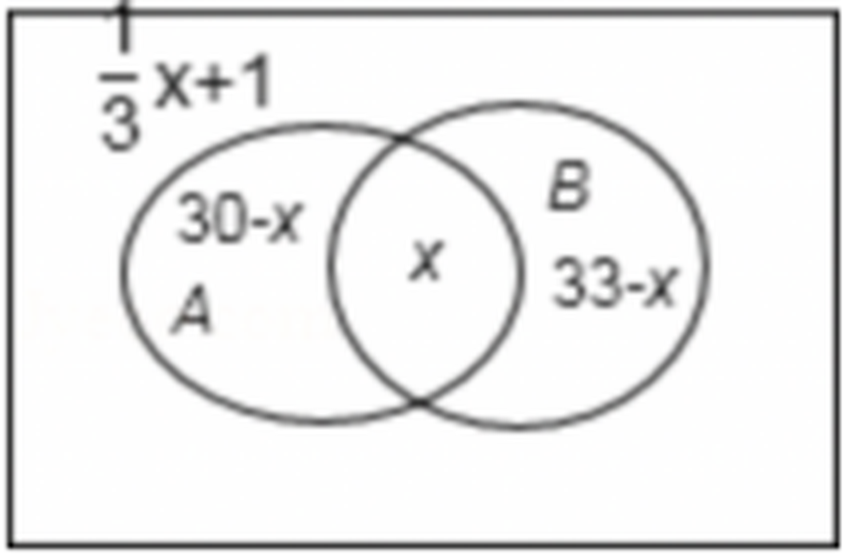
\includegraphics[width=0.30\textwidth]{figures/venn_AB_survey_50.png}
\end{center}

\ans{$21$}

\ifanswer
\solbegin
\step{由题意得赞成 $A$ 的人数 30，赞成 $B$ 的人数为 33，}
\step{设对 $A$、$B$ 都赞成的学生数为 $x$，则对 $A$、$B$ 都不赞成的学生数 $\dfrac{1}{3}x+1$，}
\step{如图得 $x+30-x+33-x+\dfrac{1}{3}x+1=50$，所以 $x=21$.}
\solend

\fi

\item 集合 $S=\{s\mid s=2n+1,n\in\Z\}$，$T=\{t\mid t=4n+1,n\in\Z\}$，则 $S$ \blankline[2.4em] $T$（填“$\subset$”“$\supset$”“$\subseteq$”或“$\supseteq$”）.

\ans{$S\supset T$}

\ifanswer
\solbegin
\step{对于 $S=\{s\mid s=2n+1,n\in\Z\}$ 为奇数，}
\step{而 $T=\{t\mid t=4n+1,n\in\Z\}$ 被 4 整除余 1 的奇数，所以 $S\supset T$.}
\solend

\fi

\item 已知集合 $A=\{x\mid -2<x<4\}$，$B=\{x\mid x^2-3ax+2a^2=0\}$，若 $A\cap B=B$，则实数 $a$ 的取值范围为 \blankline[4.4em].

\ans{$(-1,2)$}

\ifanswer
\solbegin
\step{因为 $A\cap B=B$，所以 $B\subseteq A$，}
\step{①当 $a=0$ 时，方程 $x^2-3ax+2a^2=0$ 的解为 $0$，$B\subseteq A$ 成立；}
\step{②当 $a\neq 0$ 时，方程 $x^2-3ax+2a^2=0$ 的解为 $2a$、$a$，}
\step{则 $-2<2a<4$ 且 $-2<a<4$，解得 $-1<a<2$ 且 $a\neq 0$；}
\step{综上所述，实数 $a$ 的取值范围为 $(-1,2)$.}
\solend

\fi

\item 当一个非空数集 $F$ 满足条件“若 $a$、$b\in F$，则 $a+b$、$a-b$、$ab\in F$，且当 $b\neq 0$ 时，$\dfrac{a}{b}\in F$”时，称 $F$ 为一个数域，以下四个关于数域的命题：

（1）$0$ 是任何数域的元素；（2）若数域 $F$ 有非零元素，则 $2026\in F$；

（3）集合 $P=\{x\mid x=3k,k\in\Z\}$ 为数域；（4）有理数集为数域；

其中，真命题的编号为 \blankline[4.4em]（写出所有真命题的编号）.

\ans{（1）（2）（4）}

\item 对于集合 $M$，定义函数 $f_M(x)=\begin{cases}-1,&x\in M\\ 1,&x\notin M\end{cases}$，对于两个集合 $M$、$N$，定义集合
$M\triangle N=\{x\mid f_M(x)\cdot f_N(x)=-1\}$，已知 $A=\{2,4,6,8,10\},B=\{1,2,4,8,16\}$，用 $|M|$ 表示有限集合 $M$ 中的元素个数，则对于任意集合 $M$，$|M\triangle A|+|M\triangle B|$ 的最小值为 \blankline[2.4em].

% 注：上面分段函数的第二行，原卷印作「1, $x\in M$」（两行都印 $x\in M$），与函数的定义矛盾，
%     本稿按文意订正为 $x\notin M$.
\ans{$4$}

\ifanswer
\solbegin
% 注：下面一行原卷印作「即 $M\triangle N\in\{x\mid x\in M\cup N\}$ 且 $x\in M\cap N$」，「$\in$」当为
%     「$=$」之误，且由 $f_M(x)f_N(x)=-1$ 应对应 $x\notin M\cap N$，本稿一并按文意订正.
\step{由 $M\triangle N$ 的定义得 $f_M(x)\cdot f_N(x)=-1$，}
\step{即 $M\triangle N=\{x\mid x\in M\cup N\text{ 且 }x\notin M\cap N\}$，}
\step{$|M\triangle A|+|M\triangle B|$ 要取得最小值，需满足 $A\cap B\subseteq M\subseteq A\cup B$，}
\step{此时 $|M\triangle A|+|M\triangle B|$ 的最小值为 $4$.}
\solend

\fi

\end{enumerate}

\bigsec{二、选择题}

\begin{enumerate}
\setcounter{enumi}{12}

\item 已知集合 $A=\{x\mid x=3m,m\in\N\}$，$B=\{x\mid x=3m+1,m\in\N\}$，$C=\{x\mid x=3m+2,m\in\N\}$，若 $a\in A$，$b\in B$，$c\in C$，则下列结论中可能成立的是\mbox{（\quad）}

\keepwithprev
A. $2021=a+b+c$\qquad B. $2021=abc$\qquad C. $2021=a+bc$\qquad D. $2021=a(b+c)$

\ans{C}

\ifanswer
\solbegin
\step{由题意设 $a=3m$，$b=3p+1$，$c=3n+2$，$m$、$p$、$n\in\N$，}
\step{则 $a+b+c=3m+3p+1+3n+2=3(m+p+n+1)$，}
\step{故 2021 不是 3 的整数倍，则 A 不可能；}
\step{$abc=3m(3p+1)(3n+2)$，同理 B 不可能；}
\step{$a+bc=3m+(3p+1)(3n+2)=3(m+3pn+2p+n)+2$，$2021=3\times 673+2$，}
\step{如取 $p=n=1$，则 $m=667$，即 $2021=3\times 667+4\times 5$，故 C 成立；}
\step{$a(b+c)=3m(3p+1+3n+2)=9m(p+n+1)$，同 A 可得 D 不可能.}
\step{故选 C.}
\solend

\fi

\item 设 $a$、$b$、$c$ 是实数，$x=a^2-2b+\dfrac{\pi}{3}$，$y=b^2-2c+\dfrac{\pi}{6}$，$z=c^2-2a+\dfrac{\pi}{2}$，则 $x$、$y$、$z$ 中至少有一个值\mbox{（\quad）}

\keepwithprev
A. 大于 $0$\qquad B. 等于 $0$\qquad C. 不大于 $0$\qquad D. 小于 $0$

\ans{A}

\ifanswer
\solbegin
\step{因为 $x+y+z=a^2-2b+\dfrac{\pi}{3}+b^2-2c+\dfrac{\pi}{6}+c^2-2a+\dfrac{\pi}{2}=(a-1)^2+(b-1)^2+(c-1)^2+\pi-3>0$，}
\step{假设 $x$、$y$、$z$ 都不大于 $0$，即 $x\leqslant 0$，$y\leqslant 0$，$z\leqslant 0$，}
\step{由同向不等式的可加性得 $x+y+z\leqslant 0$①，又 $x+y+z>0$ 与①式矛盾.}
\step{所以假设不成立，即原命题的结论 $x$、$y$、$z$ 中至少有一个大于 $0$. 故选 A.}
\solend

\fi

\item 命题“存在一个无理数，它的平方是有理数”的否定是\mbox{（\quad）}

\keepwithprev
A. 任意一个有理数，它的平方是有理数

B. 任意一个无理数，它的平方不是有理数

C. 存在一个有理数，它的平方是有理数

D. 存在一个无理数，它的平方不是有理数

\ans{B}

\ifanswer
\solbegin
\step{否定是任意一个无理数，它的平方不是有理数，故选 B.}
\solend

\fi

\item 设集合 $P_1=\{x\mid x^2+ax+1>0\}$，$P_2=\{x\mid x^2+ax+2>0\}$，$Q_1=\{x\mid x^2+x+b>0\}$，$Q_2=\{x\mid x^2+2x+b>0\}$，其中 $a$、$b\in\R$，下列说法正确的是\mbox{（\quad）}

\keepwithprev
A. 对任意 $a$，$P_1$ 是 $P_2$ 的子集，对任意 $b$，$Q_1$ 不是 $Q_2$ 的子集

B. 对任意 $a$，$P_1$ 是 $P_2$ 的子集，存在 $b$，使得 $Q_1$ 是 $Q_2$ 的子集

C. 对任意 $a$，使得 $P_1$ 不是 $P_2$ 的子集，对任意 $b$，$Q_1$ 不是 $Q_2$ 的子集

D. 对任意 $a$，使得 $P_1$ 不是 $P_2$ 的子集，存在 $b$，使得 $Q_1$ 不是 $Q_2$ 的子集

\ans{B}

\ifanswer
\solbegin
\step{对于集合 $P_1=\{x\mid x^2+ax+1>0\}$，$P_2=\{x\mid x^2+ax+2>0\}$，}
\step{得当 $m\in P_1$，即 $m^2+am+1>0$，得 $m^2+am+2>0$，}
\step{即有 $m\in P_2$，得对任意 $a$，$P_1$ 是 $P_2$ 的子集；}
\step{当 $b=5$ 时，$Q_1=\{x\mid x^2+x+5>0\}=\R$，$Q_2=\{x\mid x^2+2x+5>0\}=\R$，}
\step{得 $Q_1$ 是 $Q_2$ 的子集，故 A 错误，B 正确；}
\step{当 $b=1$ 时，$Q_1=\{x\mid x^2+x+1>0\}=\R$，}
\step{$Q_2=\{x\mid x^2+2x+1>0\}=\{x\mid x\neq -1\text{ 且 }x\in\R\}$，得 $Q_1$ 不是 $Q_2$ 的子集.}
\step{综上，对任意 $a$，$P_1$ 是 $P_2$ 的子集，存在 $b$，使得 $Q_1$ 是 $Q_2$ 的子集，}
\step{故 C 错误，D 错误.}
\step{故选 B.}
\solend

\fi

\end{enumerate}

\bigsec{三、解答题}

\begin{enumerate}
\setcounter{enumi}{16}

\item 已知集合 $A=\{x\mid 0<x-a\leqslant 5\}$，$B=\left\{x\mid -\dfrac{a}{2}<x\leqslant 6\right\}$.

\begin{enumerate}[label=(\arabic*)]
\item 若 $A\subseteq B$，求 $a$ 的取值范围.
\item 集合 $A$ 与 $B$ 能否相等？若能，求出 $a$ 的值，若不能，请说明理由.
\end{enumerate}

\ans{（1）$0\leqslant a\leqslant 1$；（2）不能，$a\in\varnothing$}

\ifanswer
\solbegin
\stepm{（1）}{由于 $A\subseteq B$，所以 $a+5\leqslant 6$，且 $-\dfrac{a}{2}\leqslant a$，解得 $0\leqslant a\leqslant 1$；}
\stepm{（2）}{$A=B$ 时，$a+5=6$，$-\dfrac{a}{2}=a$，解得 $a\in\varnothing$.}
\solend

\fi

\ansspace[6]

\item 已知 $\alpha:2x+m<0$，$\beta:-1<x<3$.

\begin{enumerate}[label=(\arabic*)]
\item 是否存在实数 $m$，使得 $\alpha$ 是 $\beta$ 的充分条件？若存在，求出实数 $m$ 的取值范围；
\item 是否存在实数 $m$，使得 $\alpha$ 是 $\beta$ 的必要条件？若存在，求出实数 $m$ 的取值范围.
\end{enumerate}

\ans{（1）不存在；（2）存在，$m\leqslant -6$}

\ansspace[6]

\item 已知 $\triangle ABC$ 的三边长分别为 $a,b,c$，证明：

\begin{enumerate}[label=(\arabic*)]
\item “$A=90^\circ$”是“关于 $x$ 的方程 $x^2+2ax+b^2=0$ 与 $x^2+2cx-b^2=0$ 有公共实根”的充分条件；
\item “$a=c$”是“关于 $x$ 的方程 $x^2+2ax+b^2=0$ 与 $x^2+2cx-b^2=0$ 没有公共实根”的充分非必要条件.
\end{enumerate}

\ans{（1）略；（2）略}

\ansspace[8]

\item 已知集合 $A$ 包含有 $n(n\in\N^*)$ 个元素，$A^+=\{x+y\mid x\text{、}y\in A\}$.

\begin{enumerate}[label=(\arabic*)]
\item 若 $A=\{0,1,2\}$，写出 $A^+$；
\item % 注：原卷此处印作「写出一个 $A^+$，使得 $A=A^+$」——$A$ 未给定，该问无法作答，
      %     与下方【解析】「取 $A=\{0\}$」不符，本稿按文意订正为「写出一个 $A$」.
      写出一个 $A$，使得 $A=A^+$；
\item 当 $n=4$ 时，是否存在集合 $A$，使得 $A^+=\{2,3,5,6,7,8,10\}$？若存在，求出此时的集合 $A$，若不存在，请说明理由.
\end{enumerate}

\ans{（1）$\{0,1,2,3,4\}$；（2）$A=\{0\}$；（3）不存在}

\ifanswer
\solbegin
\stepm{（1）}{由题意得 $0+0=0$，$0+1=1$，$0+2=2$，$1+1=2$，$1+2=3$，$2+2=4$ 都是 $A^+$ 中的元素，故 $A^+=\{0,1,2,3,4\}$；}
\stepm{（2）}{取 $A=\{0\}$，此时 $A^+=\{x+y\mid x\text{、}y\in A\}=\{0\}$，符合 $A=A^+$；}
\stepm{（3）}{当 $n=4$ 时，不存在集合 $A$，使得 $A^+=\{2,3,5,6,7,8,10\}$，理由如下：}
\step{假设存在 $A=\{a,b,c,d\}$，且 $a<b<c<d$，}
\step{则 $2a<a+b<a+c<b+c<b+d<c+d<2d$，}
\step{故 $2a,a+b,a+c,b+c,b+d,c+d,2d$ 为 $A^+$ 中 7 个不同的元素，}
\step{则 $2a=2$，$a+b=3$，$a+c=5$，$b+c=6$，$b+d=7$，$c+d=8$，$2d=10$，}
\step{解得 $a=1$，$b=2$，$c=4$，$d=5$，}
\step{此时 $c+d=9\in A^+$ 与 $9\notin A^+$ 矛盾，故假设不成立，}
\step{即不存在这样的集合 $A$.}
\solend

\fi

\ansspace[8]

% 压轴题：在其 \item 前先量一下版面，本页剩余高度不足 7cm 就另起一页。
\ansneed{7cm}

\item 已知集合 $A$ 为非空数集，对于集合 $A$，对 $A$ 中任意两个不同元素相加得到的和取绝对值，将这些绝对值重新组成一个新的集合，对于这一过程，我们定义为“自相加”，重新组成的集合叫做“集合 $A$ 的 1 次自相加集合”，再进行 $n-1$ 次“自相加”操作，组成的集合叫做“集合 $A$ 的 $n$ 次自相加集合”. 若集合 $A$ 的任意 $k$ 次自相加集合都不相等，则称集合 $A$ 为“完美自相加集合”，同理，我们可以定义出“$A$ 的 1 次自相减集合”，集合 $A$ 的 1 次自相加集合和 1 次自相减集合分别可表示为：$A^+=\{x\mid x=|a+b|,\ a\text{、}b\in A\}$，$A^-=\{x\mid x=|a-b|,\ a\text{、}b\in A\}$.

\begin{enumerate}[label=(\arabic*)]
\item 已知有两个集合，集合 $B=\{1,2,3,4\}$，集合 $C=\{k\mid k=2n+1,n\in\Z\}$，判断集合 $B$ 和集合 $C$ 是否是完美自相加集合，并说明理由；
\item 对（1）中的集合 $B$ 进行 11 次自相加操作后，求：集合 $B$ 的 11 次自相加集合的元素个数；
\item 若 $0\leqslant n\leqslant 2025$ 且 $n\in\N$，集合 $A=\{x\mid n\leqslant x\leqslant 2025,x\in\N\}$，$A^+\cap A^-=\varnothing$，求：$n$ 的最小值.
\end{enumerate}

\ans{（1）$B$ 是完美自相加集合，$C$ 不是完美自相加集合；（2）$2051$；（3）$675$}

\ifanswer
\solbegin
\stepm{（1）}{$B$ 是完美自相加集合，$C$ 不是完美自相加集合，}
\step{理由如下：因为集合 $B=\{1,2,3,4\}$，所以 $B^+=\{3,4,5,6,7\}$，}
\step{由此可得集合自相加后，}
\step{新的集合中最小的元素为自相加之前的集合中的最小两个元素之和，}
\step{所以显然集合 $B=\{1,2,3,4\}$ 的最小两个元素为 $1$，$2$，}
\step{所以 $B^+$ 中的最小元素为 $1+2=3$，}
\step{同理，2 次自相加后得到的集合中的最小元素是 $3+4=7$.}
\step{依照这样的规律，对集合 $B=\{1,2,3,4\}$ 进行任意次自相加操作后，}
\step{最小值总在变大，故不可能有相等集合，所以 $B$ 是完美自相加集合；}
\step{因为集合 $C=\{k\mid k=2n+1,n\in\Z\}$ 表示所有奇数构成的集合，}
\step{任何两个奇数相加的和都是偶数，}
\step{所以 $C^+=\{k\mid k=2n,n\in\Z\}$ 为所有偶数构成集合；}
\step{所以对 $C^+=\{k\mid k=2n,n\in\Z\}$ 再进行一次自相加操作，}
\step{因为任意两个偶数相加的和还是偶数，}
\step{所以后面集合不管进行多少次相加都与 $C^+=\{k\mid k=2n,n\in\Z\}$ 相同；}
\step{故 $C$ 不是完美自相加集合.}
\stepm{（2）}{由自相加性质得，对于集合 $B=\{1,2,3,4\}$，进行一次自相加，}
\step{得到集合的最小值必然是原来集合的两个最小元素值之和，}
\step{得到的最大值必然为原来集合的两个最大元素值之和，}
\step{且中间必然是连续的整数元素；}
\step{所以对集合 $B=\{1,2,3,4\}$ 进行 1 次自相加之后，}
\step{得到的集合最小两个元素为 $3$，$4$，最大的两个元素为 $6$，$7$；}
\step{进行第 2 次自相加，得到的集合最小两个元素为 $7$，$8$，}
\step{最大的两个元素为 $12$，$13$；}
\step{进行第 3 次自相加，得到的集合最小两个元素为 $15$，$16$，}
\step{最大的两个元素为 $24$，$25$；}
\step{进行第 4 次自相加，得到的集合最小两个元素为 $31$，$32$，}
\step{最大的两个元素为 $48$，$49$；}
\step{进行第 5 次自相加，得到的集合最小两个元素为 $63$，$64$，}
\step{最大的两个元素为 $96$，$97$；}
\step{进行第 6 次自相加，得到的集合最小两个元素为 $127$，$128$，}
\step{最大的两个元素为 $192$，$193$；}
\step{进行第 7 次自相加，得到的集合最小两个元素为 $255$，$256$，}
\step{最大的两个元素为 $384$，$385$；}
\step{进行第 8 次自相加，得到的集合最小两个元素为 $511$，$512$，}
\step{最大的两个元素为 $768$，$769$；}
\step{进行第 9 次自相加，得到的集合最小两个元素为 $1023$，$1024$，}
\step{最大的两个元素为 $1536$，$1537$；}
\step{进行第 10 次自相加，得到的集合最小两个元素为 $2047$，$2048$，}
\step{最大的两个元素为 $3072$，$3073$；}
\step{进行第 11 次自相加，得到的集合最小两个元素为 $4095$，$4096$，}
\step{最大的两个元素为 $6144$，$6145$；}
\step{因为集合 $B$ 的 $n$ 次自相加集合中的元素都是连续的整数，}
\step{所以集合 $B$ 进行 11 次自相加操作后的元素个数为 $6145-4095+1=2051$.}
\stepm{（3）}{因为 $0\leqslant n\leqslant 2025$ 且 $n\in\N$，集合 $A=\{x\mid n\leqslant x\leqslant 2025,x\in\N\}$，}
\step{所以 $A^+=\{x\mid 2n+1\leqslant x\leqslant 4049,x\in\N\}$，}
\step{$A^-=\{x\mid 1\leqslant x\leqslant 2025-n,x\in\N\}$，}
\step{要使 $A^+\cap A^-=\varnothing$，须使 $2n+1>2025-n$，所以 $n>\dfrac{2024}{3}=674\dfrac{2}{3}$，}
\step{又 $n\in\N$，故 $n$ 的最小值为 $675$.}
\solend

\fi

% 压轴题：其后已无内容，故作答区全用可丢弃胶水（\ansspace*）。
\ansspace*[12]

\end{enumerate}

\end{document}
"
% 紧凑版：xelatex "\def\iscompact{1}% 高一17_七宝中学_周末作业2.tex —— 高一上数学「2026-2027 年七宝中学高一上周末作业 2」（试卷版/答案版）
% 试卷版：xelatex 高一17_七宝中学_周末作业2.tex
% 答案版：xelatex "\def\isanswer{1}% 高一17_七宝中学_周末作业2.tex —— 高一上数学「2026-2027 年七宝中学高一上周末作业 2」（试卷版/答案版）
% 试卷版：xelatex 高一17_七宝中学_周末作业2.tex
% 答案版：xelatex "\def\isanswer{1}\input{高一17_七宝中学_周末作业2.tex}"
% 紧凑版：xelatex "\def\iscompact{1}\input{高一17_七宝中学_周末作业2.tex}"
%
% 原始材料是微信公众号图文（公众号「魔都数学加油站」），正文为 10 张 PNG 页（1080×1527）。
% 原文本身就是一份**讲评版**——题目下方直接印出【答案】或【解析】，选择题的答案印在解析末句
% 「故选 X」里。试题文字、答案与解析均照原卷录入（订正处见下），卷面上的粉色斜水印
% 「魔都数学加油站」属水印，未录入。
%
% 与原卷的排版差异（均已在 README「说明」中交代）：
%   ① 原文自**第 3 题**起（第 1、2 题未在该文中发布），故本稿题号亦自 3 起；
%   ② 原卷本就印有「一、填空题」「二、选择题」「三、解答题」三节标题（分别在原图 00/02/04.png
%      上，逐页核对过），本稿照原卷分节，只把标题改排成全稿统一的「大节标题」样式；
%   ③ 原卷填空、选择的答案直接印在题目下方（选择题只在解析末句「故选 X」中给出），本稿统一改为
%      试卷版隐去、答案版以【答案】给出，选择题的括注一律改排「\mbox{（\quad）}」并把答案移到选项之后，
%      使两版彻底分离；
%   ④ 原卷的集合符号大小写混用：第 3 题题干的实数集印成**粗体** $\mathbf{R}$，第 16 题题干与
%      第 16 题解析的印成正体 $R$；自然数集 $N$、整数集 $Z$ 一律正体。本稿按全稿惯例统一写作
%      $\R$、$\N$、$\Z$；
%   ⑤ 原卷未印副标题，本稿按全稿惯例补出副标题「集合与常用逻辑用语」；
%   ⑥ 原卷解答题子问编号为「（1）（2）」，本稿用嵌套 enumerate 排成同一形态；原卷第 15 题的
%      D 选项因原页翻页被截到下一页首页，本稿自然连排；
%   ⑦ 原卷解答题未留作答空间（讲评稿通篇是答案），本稿逐题补出书写留白，仅试卷版显示；
%   ⑧ 第 21 题题干里 $A^+$、$A^-$ 的定义含绝对值号（原卷作 $\{x\mid x=|a+b|,\ a\text{、}b\in A\}$
%      与 $\{x\mid x=|a-b|,\ a\text{、}b\in A\}$），本稿照原卷录入；2026-09-15 回原图逐处放大复核
%      时发现曾漏抄两处绝对值号、并把分隔逗号误写成 $\mid$，已按原卷订正（见 README 专记）。
%
% 原卷笔误三处（均已放大到能看清字形后核对，本稿按文意订正，并在 README 中写明原委）：
%   ① 第 12 题题干的分段函数 $f_M(x)$ 原卷两行都印作「$x\in M$」（$-1$ 与 $1$ 都取在 $M$ 上），
%      与「函数」的定义直接矛盾（$M$ 上无法同时取两个值），按文意订正第二行为 $x\notin M$；
%   ② 第 12 题【解析】首行原卷印「即 $M\triangle N\in\{x\mid x\in M\cup N\}$ 且 $x\in M\cap N$」，
%      其中「$\in$」当为「$=$」之误；且由 $f_M(x)f_N(x)=-1$ 应对应 $x\notin M\cap N$（原卷印作
%      $x\in M\cap N$，与上一行刚写出的对称差的定义相矛盾），本稿一并订正；
%   ③ 第 20 题(2)原卷印「写出一个 $A^+$，使得 $A=A^+$」——$A$ 未给定，该问无法作答，与紧接的
%      【解析】「取 $A=\{0\}$，此时 $A^+=\{0\}$，符合 $A=A^+$」不符，本稿按文意订正为
%      「写出一个 $A$，使得 $A=A^+$」.
%
% 原卷存疑一处（无法确证原意，本稿照抄原卷、未改）：
%   ① 第 5 题 ④ 原卷题干印 $S=\{x\mid |x|\leqslant\sqrt{3},x\in N\}$（该字母与 ③ 中的 $Z$
%      字形明显不同，$Z$ 有上下两横，已放大比对确认），而【解析】印「因为 $S=\{-1,0,1\}$」——
%      按 $x\in N$ 应为 $S=\{0,1\}$（或 $\{1\}$），题干与解析的口径不一致；但无论取哪一口径，
%      ④ 都是 $M$ 的子集、本题结论（填④）不变，故题干与解析均照抄原卷，未改。

\documentclass[a4paper,11pt]{article}
\usepackage{common}

\begin{document}

\examtitlest{2026--2027 年七宝中学高一上周末作业 2}{集合与常用逻辑用语}

\bigsec{一、填空题}

\begin{enumerate}
\setcounter{enumi}{2}

\item 已知 $a,x\in\R$，则“$x\in\{-a,a\}$”是“$|x|=a$”的 \blankline[4.4em] 条件.

\ans{必要不充分}

\item 设全集为 $U$，$A\subseteq U$，$B\subseteq U$，则“$A\subset B$”是“$\overline{B}\subset\overline{A}$”的 \blankline[4.4em] 条件.

\ans{充要}

\item 已知集合 $M=\{x\mid -\sqrt{5}<x<\sqrt{3},x\in\Z\}$，则下列集合是集合 $M$ 的子集的是 \blankline[4.4em]（填序号）.

① $P=\{-3,0,1\}$；② $Q=\{-1,0,1,2\}$；③ $R=\{y\mid -\pi<y<-1,y\in\Z\}$；

④ $S=\{x\mid |x|\leqslant\sqrt{3},x\in\N\}$.

\ans{④}

\ifanswer
\solbegin
\step{由已知得集合 $M=\{-2,-1,0,1\}$，}
\step{所以由子集的定义得选项①错误，②错误，}
\step{因为 $R=\{-3,-2\}$，所以集合 $R$ 不表示集合 $M$ 的子集，③错误，}
\step{因为 $S=\{-1,0,1\}$，所以是集合 $M$ 的子集，故正确.}
\step{故是集合 $M$ 的子集的是④.}
\solend

\fi

\item 已知 $x\in\R$，用反证法证明命题“若 $x^2-7x+10<0$，则 $2<x<5$”时，应该假设 \blankline[5em].

\ans{$x\leqslant 2$ 或 $x\geqslant 5$}

\item 设 $a_1,b_1,c_1,a_2,b_2,c_2$ 均为非零实数，方程 $a_1x^2+b_1x+c_1=0$ 和 $a_2x^2+b_2x+c_2=0$ 的解集分别为 $M$ 和 $N$，那么“$\dfrac{a_1}{a_2}=\dfrac{b_1}{b_2}=\dfrac{c_1}{c_2}$”是“$M=N$”的 \blankline[4.4em] 条件.

（填“充分非必要”、“必要非充分”、“充要”、或“既非充分又非必要”）

\ans{充分非必要}

\ifanswer
\solbegin
\step{$\dfrac{a_1}{a_2}=\dfrac{b_1}{b_2}=\dfrac{c_1}{c_2}$ 能推出 $M=N$，}
\step{若 $M=N=\varnothing$ 推不出 $\dfrac{a_1}{a_2}=\dfrac{b_1}{b_2}=\dfrac{c_1}{c_2}$，}
\step{所以“$\dfrac{a_1}{a_2}=\dfrac{b_1}{b_2}=\dfrac{c_1}{c_2}$”是“$M=N$”的“充分非必要”条件.}
\solend

\fi

\item 向 50 名学生调查对 $A$、$B$ 两事件的态度，有如下结果赞成 $A$ 的人数是全体的五分之三，其余的不赞成，赞成 $B$ 的比赞成 $A$ 的多 3 人，其余的不赞成；另外，对 $A$、$B$ 都不赞成的学生数比对 $A$、$B$ 都赞成的学生数的三分之一多 1 人. 则对 $A$、$B$ 都赞成的学生有 \blankline[2.4em] 人.

\begin{center}
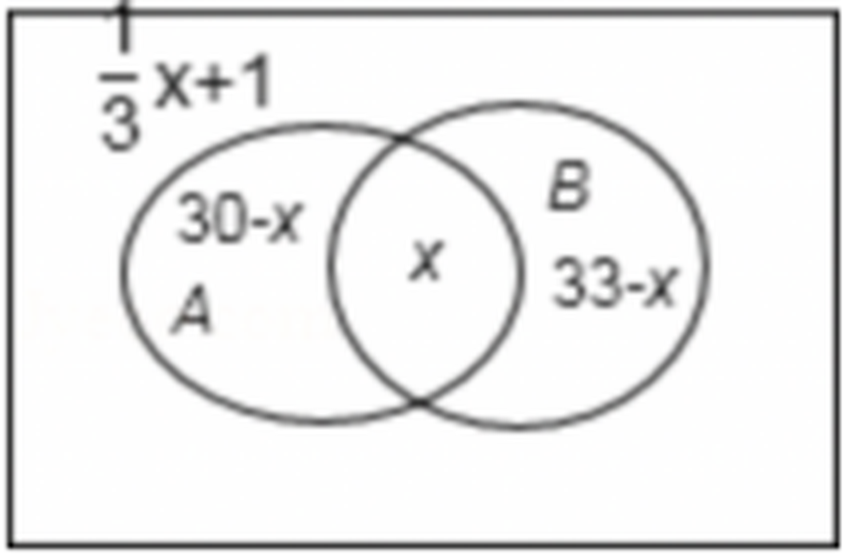
\includegraphics[width=0.30\textwidth]{figures/venn_AB_survey_50.png}
\end{center}

\ans{$21$}

\ifanswer
\solbegin
\step{由题意得赞成 $A$ 的人数 30，赞成 $B$ 的人数为 33，}
\step{设对 $A$、$B$ 都赞成的学生数为 $x$，则对 $A$、$B$ 都不赞成的学生数 $\dfrac{1}{3}x+1$，}
\step{如图得 $x+30-x+33-x+\dfrac{1}{3}x+1=50$，所以 $x=21$.}
\solend

\fi

\item 集合 $S=\{s\mid s=2n+1,n\in\Z\}$，$T=\{t\mid t=4n+1,n\in\Z\}$，则 $S$ \blankline[2.4em] $T$（填“$\subset$”“$\supset$”“$\subseteq$”或“$\supseteq$”）.

\ans{$S\supset T$}

\ifanswer
\solbegin
\step{对于 $S=\{s\mid s=2n+1,n\in\Z\}$ 为奇数，}
\step{而 $T=\{t\mid t=4n+1,n\in\Z\}$ 被 4 整除余 1 的奇数，所以 $S\supset T$.}
\solend

\fi

\item 已知集合 $A=\{x\mid -2<x<4\}$，$B=\{x\mid x^2-3ax+2a^2=0\}$，若 $A\cap B=B$，则实数 $a$ 的取值范围为 \blankline[4.4em].

\ans{$(-1,2)$}

\ifanswer
\solbegin
\step{因为 $A\cap B=B$，所以 $B\subseteq A$，}
\step{①当 $a=0$ 时，方程 $x^2-3ax+2a^2=0$ 的解为 $0$，$B\subseteq A$ 成立；}
\step{②当 $a\neq 0$ 时，方程 $x^2-3ax+2a^2=0$ 的解为 $2a$、$a$，}
\step{则 $-2<2a<4$ 且 $-2<a<4$，解得 $-1<a<2$ 且 $a\neq 0$；}
\step{综上所述，实数 $a$ 的取值范围为 $(-1,2)$.}
\solend

\fi

\item 当一个非空数集 $F$ 满足条件“若 $a$、$b\in F$，则 $a+b$、$a-b$、$ab\in F$，且当 $b\neq 0$ 时，$\dfrac{a}{b}\in F$”时，称 $F$ 为一个数域，以下四个关于数域的命题：

（1）$0$ 是任何数域的元素；（2）若数域 $F$ 有非零元素，则 $2026\in F$；

（3）集合 $P=\{x\mid x=3k,k\in\Z\}$ 为数域；（4）有理数集为数域；

其中，真命题的编号为 \blankline[4.4em]（写出所有真命题的编号）.

\ans{（1）（2）（4）}

\item 对于集合 $M$，定义函数 $f_M(x)=\begin{cases}-1,&x\in M\\ 1,&x\notin M\end{cases}$，对于两个集合 $M$、$N$，定义集合
$M\triangle N=\{x\mid f_M(x)\cdot f_N(x)=-1\}$，已知 $A=\{2,4,6,8,10\},B=\{1,2,4,8,16\}$，用 $|M|$ 表示有限集合 $M$ 中的元素个数，则对于任意集合 $M$，$|M\triangle A|+|M\triangle B|$ 的最小值为 \blankline[2.4em].

% 注：上面分段函数的第二行，原卷印作「1, $x\in M$」（两行都印 $x\in M$），与函数的定义矛盾，
%     本稿按文意订正为 $x\notin M$.
\ans{$4$}

\ifanswer
\solbegin
% 注：下面一行原卷印作「即 $M\triangle N\in\{x\mid x\in M\cup N\}$ 且 $x\in M\cap N$」，「$\in$」当为
%     「$=$」之误，且由 $f_M(x)f_N(x)=-1$ 应对应 $x\notin M\cap N$，本稿一并按文意订正.
\step{由 $M\triangle N$ 的定义得 $f_M(x)\cdot f_N(x)=-1$，}
\step{即 $M\triangle N=\{x\mid x\in M\cup N\text{ 且 }x\notin M\cap N\}$，}
\step{$|M\triangle A|+|M\triangle B|$ 要取得最小值，需满足 $A\cap B\subseteq M\subseteq A\cup B$，}
\step{此时 $|M\triangle A|+|M\triangle B|$ 的最小值为 $4$.}
\solend

\fi

\end{enumerate}

\bigsec{二、选择题}

\begin{enumerate}
\setcounter{enumi}{12}

\item 已知集合 $A=\{x\mid x=3m,m\in\N\}$，$B=\{x\mid x=3m+1,m\in\N\}$，$C=\{x\mid x=3m+2,m\in\N\}$，若 $a\in A$，$b\in B$，$c\in C$，则下列结论中可能成立的是\mbox{（\quad）}

\keepwithprev
A. $2021=a+b+c$\qquad B. $2021=abc$\qquad C. $2021=a+bc$\qquad D. $2021=a(b+c)$

\ans{C}

\ifanswer
\solbegin
\step{由题意设 $a=3m$，$b=3p+1$，$c=3n+2$，$m$、$p$、$n\in\N$，}
\step{则 $a+b+c=3m+3p+1+3n+2=3(m+p+n+1)$，}
\step{故 2021 不是 3 的整数倍，则 A 不可能；}
\step{$abc=3m(3p+1)(3n+2)$，同理 B 不可能；}
\step{$a+bc=3m+(3p+1)(3n+2)=3(m+3pn+2p+n)+2$，$2021=3\times 673+2$，}
\step{如取 $p=n=1$，则 $m=667$，即 $2021=3\times 667+4\times 5$，故 C 成立；}
\step{$a(b+c)=3m(3p+1+3n+2)=9m(p+n+1)$，同 A 可得 D 不可能.}
\step{故选 C.}
\solend

\fi

\item 设 $a$、$b$、$c$ 是实数，$x=a^2-2b+\dfrac{\pi}{3}$，$y=b^2-2c+\dfrac{\pi}{6}$，$z=c^2-2a+\dfrac{\pi}{2}$，则 $x$、$y$、$z$ 中至少有一个值\mbox{（\quad）}

\keepwithprev
A. 大于 $0$\qquad B. 等于 $0$\qquad C. 不大于 $0$\qquad D. 小于 $0$

\ans{A}

\ifanswer
\solbegin
\step{因为 $x+y+z=a^2-2b+\dfrac{\pi}{3}+b^2-2c+\dfrac{\pi}{6}+c^2-2a+\dfrac{\pi}{2}=(a-1)^2+(b-1)^2+(c-1)^2+\pi-3>0$，}
\step{假设 $x$、$y$、$z$ 都不大于 $0$，即 $x\leqslant 0$，$y\leqslant 0$，$z\leqslant 0$，}
\step{由同向不等式的可加性得 $x+y+z\leqslant 0$①，又 $x+y+z>0$ 与①式矛盾.}
\step{所以假设不成立，即原命题的结论 $x$、$y$、$z$ 中至少有一个大于 $0$. 故选 A.}
\solend

\fi

\item 命题“存在一个无理数，它的平方是有理数”的否定是\mbox{（\quad）}

\keepwithprev
A. 任意一个有理数，它的平方是有理数

B. 任意一个无理数，它的平方不是有理数

C. 存在一个有理数，它的平方是有理数

D. 存在一个无理数，它的平方不是有理数

\ans{B}

\ifanswer
\solbegin
\step{否定是任意一个无理数，它的平方不是有理数，故选 B.}
\solend

\fi

\item 设集合 $P_1=\{x\mid x^2+ax+1>0\}$，$P_2=\{x\mid x^2+ax+2>0\}$，$Q_1=\{x\mid x^2+x+b>0\}$，$Q_2=\{x\mid x^2+2x+b>0\}$，其中 $a$、$b\in\R$，下列说法正确的是\mbox{（\quad）}

\keepwithprev
A. 对任意 $a$，$P_1$ 是 $P_2$ 的子集，对任意 $b$，$Q_1$ 不是 $Q_2$ 的子集

B. 对任意 $a$，$P_1$ 是 $P_2$ 的子集，存在 $b$，使得 $Q_1$ 是 $Q_2$ 的子集

C. 对任意 $a$，使得 $P_1$ 不是 $P_2$ 的子集，对任意 $b$，$Q_1$ 不是 $Q_2$ 的子集

D. 对任意 $a$，使得 $P_1$ 不是 $P_2$ 的子集，存在 $b$，使得 $Q_1$ 不是 $Q_2$ 的子集

\ans{B}

\ifanswer
\solbegin
\step{对于集合 $P_1=\{x\mid x^2+ax+1>0\}$，$P_2=\{x\mid x^2+ax+2>0\}$，}
\step{得当 $m\in P_1$，即 $m^2+am+1>0$，得 $m^2+am+2>0$，}
\step{即有 $m\in P_2$，得对任意 $a$，$P_1$ 是 $P_2$ 的子集；}
\step{当 $b=5$ 时，$Q_1=\{x\mid x^2+x+5>0\}=\R$，$Q_2=\{x\mid x^2+2x+5>0\}=\R$，}
\step{得 $Q_1$ 是 $Q_2$ 的子集，故 A 错误，B 正确；}
\step{当 $b=1$ 时，$Q_1=\{x\mid x^2+x+1>0\}=\R$，}
\step{$Q_2=\{x\mid x^2+2x+1>0\}=\{x\mid x\neq -1\text{ 且 }x\in\R\}$，得 $Q_1$ 不是 $Q_2$ 的子集.}
\step{综上，对任意 $a$，$P_1$ 是 $P_2$ 的子集，存在 $b$，使得 $Q_1$ 是 $Q_2$ 的子集，}
\step{故 C 错误，D 错误.}
\step{故选 B.}
\solend

\fi

\end{enumerate}

\bigsec{三、解答题}

\begin{enumerate}
\setcounter{enumi}{16}

\item 已知集合 $A=\{x\mid 0<x-a\leqslant 5\}$，$B=\left\{x\mid -\dfrac{a}{2}<x\leqslant 6\right\}$.

\begin{enumerate}[label=(\arabic*)]
\item 若 $A\subseteq B$，求 $a$ 的取值范围.
\item 集合 $A$ 与 $B$ 能否相等？若能，求出 $a$ 的值，若不能，请说明理由.
\end{enumerate}

\ans{（1）$0\leqslant a\leqslant 1$；（2）不能，$a\in\varnothing$}

\ifanswer
\solbegin
\stepm{（1）}{由于 $A\subseteq B$，所以 $a+5\leqslant 6$，且 $-\dfrac{a}{2}\leqslant a$，解得 $0\leqslant a\leqslant 1$；}
\stepm{（2）}{$A=B$ 时，$a+5=6$，$-\dfrac{a}{2}=a$，解得 $a\in\varnothing$.}
\solend

\fi

\ansspace[6]

\item 已知 $\alpha:2x+m<0$，$\beta:-1<x<3$.

\begin{enumerate}[label=(\arabic*)]
\item 是否存在实数 $m$，使得 $\alpha$ 是 $\beta$ 的充分条件？若存在，求出实数 $m$ 的取值范围；
\item 是否存在实数 $m$，使得 $\alpha$ 是 $\beta$ 的必要条件？若存在，求出实数 $m$ 的取值范围.
\end{enumerate}

\ans{（1）不存在；（2）存在，$m\leqslant -6$}

\ansspace[6]

\item 已知 $\triangle ABC$ 的三边长分别为 $a,b,c$，证明：

\begin{enumerate}[label=(\arabic*)]
\item “$A=90^\circ$”是“关于 $x$ 的方程 $x^2+2ax+b^2=0$ 与 $x^2+2cx-b^2=0$ 有公共实根”的充分条件；
\item “$a=c$”是“关于 $x$ 的方程 $x^2+2ax+b^2=0$ 与 $x^2+2cx-b^2=0$ 没有公共实根”的充分非必要条件.
\end{enumerate}

\ans{（1）略；（2）略}

\ansspace[8]

\item 已知集合 $A$ 包含有 $n(n\in\N^*)$ 个元素，$A^+=\{x+y\mid x\text{、}y\in A\}$.

\begin{enumerate}[label=(\arabic*)]
\item 若 $A=\{0,1,2\}$，写出 $A^+$；
\item % 注：原卷此处印作「写出一个 $A^+$，使得 $A=A^+$」——$A$ 未给定，该问无法作答，
      %     与下方【解析】「取 $A=\{0\}$」不符，本稿按文意订正为「写出一个 $A$」.
      写出一个 $A$，使得 $A=A^+$；
\item 当 $n=4$ 时，是否存在集合 $A$，使得 $A^+=\{2,3,5,6,7,8,10\}$？若存在，求出此时的集合 $A$，若不存在，请说明理由.
\end{enumerate}

\ans{（1）$\{0,1,2,3,4\}$；（2）$A=\{0\}$；（3）不存在}

\ifanswer
\solbegin
\stepm{（1）}{由题意得 $0+0=0$，$0+1=1$，$0+2=2$，$1+1=2$，$1+2=3$，$2+2=4$ 都是 $A^+$ 中的元素，故 $A^+=\{0,1,2,3,4\}$；}
\stepm{（2）}{取 $A=\{0\}$，此时 $A^+=\{x+y\mid x\text{、}y\in A\}=\{0\}$，符合 $A=A^+$；}
\stepm{（3）}{当 $n=4$ 时，不存在集合 $A$，使得 $A^+=\{2,3,5,6,7,8,10\}$，理由如下：}
\step{假设存在 $A=\{a,b,c,d\}$，且 $a<b<c<d$，}
\step{则 $2a<a+b<a+c<b+c<b+d<c+d<2d$，}
\step{故 $2a,a+b,a+c,b+c,b+d,c+d,2d$ 为 $A^+$ 中 7 个不同的元素，}
\step{则 $2a=2$，$a+b=3$，$a+c=5$，$b+c=6$，$b+d=7$，$c+d=8$，$2d=10$，}
\step{解得 $a=1$，$b=2$，$c=4$，$d=5$，}
\step{此时 $c+d=9\in A^+$ 与 $9\notin A^+$ 矛盾，故假设不成立，}
\step{即不存在这样的集合 $A$.}
\solend

\fi

\ansspace[8]

% 压轴题：在其 \item 前先量一下版面，本页剩余高度不足 7cm 就另起一页。
\ansneed{7cm}

\item 已知集合 $A$ 为非空数集，对于集合 $A$，对 $A$ 中任意两个不同元素相加得到的和取绝对值，将这些绝对值重新组成一个新的集合，对于这一过程，我们定义为“自相加”，重新组成的集合叫做“集合 $A$ 的 1 次自相加集合”，再进行 $n-1$ 次“自相加”操作，组成的集合叫做“集合 $A$ 的 $n$ 次自相加集合”. 若集合 $A$ 的任意 $k$ 次自相加集合都不相等，则称集合 $A$ 为“完美自相加集合”，同理，我们可以定义出“$A$ 的 1 次自相减集合”，集合 $A$ 的 1 次自相加集合和 1 次自相减集合分别可表示为：$A^+=\{x\mid x=|a+b|,\ a\text{、}b\in A\}$，$A^-=\{x\mid x=|a-b|,\ a\text{、}b\in A\}$.

\begin{enumerate}[label=(\arabic*)]
\item 已知有两个集合，集合 $B=\{1,2,3,4\}$，集合 $C=\{k\mid k=2n+1,n\in\Z\}$，判断集合 $B$ 和集合 $C$ 是否是完美自相加集合，并说明理由；
\item 对（1）中的集合 $B$ 进行 11 次自相加操作后，求：集合 $B$ 的 11 次自相加集合的元素个数；
\item 若 $0\leqslant n\leqslant 2025$ 且 $n\in\N$，集合 $A=\{x\mid n\leqslant x\leqslant 2025,x\in\N\}$，$A^+\cap A^-=\varnothing$，求：$n$ 的最小值.
\end{enumerate}

\ans{（1）$B$ 是完美自相加集合，$C$ 不是完美自相加集合；（2）$2051$；（3）$675$}

\ifanswer
\solbegin
\stepm{（1）}{$B$ 是完美自相加集合，$C$ 不是完美自相加集合，}
\step{理由如下：因为集合 $B=\{1,2,3,4\}$，所以 $B^+=\{3,4,5,6,7\}$，}
\step{由此可得集合自相加后，}
\step{新的集合中最小的元素为自相加之前的集合中的最小两个元素之和，}
\step{所以显然集合 $B=\{1,2,3,4\}$ 的最小两个元素为 $1$，$2$，}
\step{所以 $B^+$ 中的最小元素为 $1+2=3$，}
\step{同理，2 次自相加后得到的集合中的最小元素是 $3+4=7$.}
\step{依照这样的规律，对集合 $B=\{1,2,3,4\}$ 进行任意次自相加操作后，}
\step{最小值总在变大，故不可能有相等集合，所以 $B$ 是完美自相加集合；}
\step{因为集合 $C=\{k\mid k=2n+1,n\in\Z\}$ 表示所有奇数构成的集合，}
\step{任何两个奇数相加的和都是偶数，}
\step{所以 $C^+=\{k\mid k=2n,n\in\Z\}$ 为所有偶数构成集合；}
\step{所以对 $C^+=\{k\mid k=2n,n\in\Z\}$ 再进行一次自相加操作，}
\step{因为任意两个偶数相加的和还是偶数，}
\step{所以后面集合不管进行多少次相加都与 $C^+=\{k\mid k=2n,n\in\Z\}$ 相同；}
\step{故 $C$ 不是完美自相加集合.}
\stepm{（2）}{由自相加性质得，对于集合 $B=\{1,2,3,4\}$，进行一次自相加，}
\step{得到集合的最小值必然是原来集合的两个最小元素值之和，}
\step{得到的最大值必然为原来集合的两个最大元素值之和，}
\step{且中间必然是连续的整数元素；}
\step{所以对集合 $B=\{1,2,3,4\}$ 进行 1 次自相加之后，}
\step{得到的集合最小两个元素为 $3$，$4$，最大的两个元素为 $6$，$7$；}
\step{进行第 2 次自相加，得到的集合最小两个元素为 $7$，$8$，}
\step{最大的两个元素为 $12$，$13$；}
\step{进行第 3 次自相加，得到的集合最小两个元素为 $15$，$16$，}
\step{最大的两个元素为 $24$，$25$；}
\step{进行第 4 次自相加，得到的集合最小两个元素为 $31$，$32$，}
\step{最大的两个元素为 $48$，$49$；}
\step{进行第 5 次自相加，得到的集合最小两个元素为 $63$，$64$，}
\step{最大的两个元素为 $96$，$97$；}
\step{进行第 6 次自相加，得到的集合最小两个元素为 $127$，$128$，}
\step{最大的两个元素为 $192$，$193$；}
\step{进行第 7 次自相加，得到的集合最小两个元素为 $255$，$256$，}
\step{最大的两个元素为 $384$，$385$；}
\step{进行第 8 次自相加，得到的集合最小两个元素为 $511$，$512$，}
\step{最大的两个元素为 $768$，$769$；}
\step{进行第 9 次自相加，得到的集合最小两个元素为 $1023$，$1024$，}
\step{最大的两个元素为 $1536$，$1537$；}
\step{进行第 10 次自相加，得到的集合最小两个元素为 $2047$，$2048$，}
\step{最大的两个元素为 $3072$，$3073$；}
\step{进行第 11 次自相加，得到的集合最小两个元素为 $4095$，$4096$，}
\step{最大的两个元素为 $6144$，$6145$；}
\step{因为集合 $B$ 的 $n$ 次自相加集合中的元素都是连续的整数，}
\step{所以集合 $B$ 进行 11 次自相加操作后的元素个数为 $6145-4095+1=2051$.}
\stepm{（3）}{因为 $0\leqslant n\leqslant 2025$ 且 $n\in\N$，集合 $A=\{x\mid n\leqslant x\leqslant 2025,x\in\N\}$，}
\step{所以 $A^+=\{x\mid 2n+1\leqslant x\leqslant 4049,x\in\N\}$，}
\step{$A^-=\{x\mid 1\leqslant x\leqslant 2025-n,x\in\N\}$，}
\step{要使 $A^+\cap A^-=\varnothing$，须使 $2n+1>2025-n$，所以 $n>\dfrac{2024}{3}=674\dfrac{2}{3}$，}
\step{又 $n\in\N$，故 $n$ 的最小值为 $675$.}
\solend

\fi

% 压轴题：其后已无内容，故作答区全用可丢弃胶水（\ansspace*）。
\ansspace*[12]

\end{enumerate}

\end{document}
"
% 紧凑版：xelatex "\def\iscompact{1}% 高一17_七宝中学_周末作业2.tex —— 高一上数学「2026-2027 年七宝中学高一上周末作业 2」（试卷版/答案版）
% 试卷版：xelatex 高一17_七宝中学_周末作业2.tex
% 答案版：xelatex "\def\isanswer{1}\input{高一17_七宝中学_周末作业2.tex}"
% 紧凑版：xelatex "\def\iscompact{1}\input{高一17_七宝中学_周末作业2.tex}"
%
% 原始材料是微信公众号图文（公众号「魔都数学加油站」），正文为 10 张 PNG 页（1080×1527）。
% 原文本身就是一份**讲评版**——题目下方直接印出【答案】或【解析】，选择题的答案印在解析末句
% 「故选 X」里。试题文字、答案与解析均照原卷录入（订正处见下），卷面上的粉色斜水印
% 「魔都数学加油站」属水印，未录入。
%
% 与原卷的排版差异（均已在 README「说明」中交代）：
%   ① 原文自**第 3 题**起（第 1、2 题未在该文中发布），故本稿题号亦自 3 起；
%   ② 原卷本就印有「一、填空题」「二、选择题」「三、解答题」三节标题（分别在原图 00/02/04.png
%      上，逐页核对过），本稿照原卷分节，只把标题改排成全稿统一的「大节标题」样式；
%   ③ 原卷填空、选择的答案直接印在题目下方（选择题只在解析末句「故选 X」中给出），本稿统一改为
%      试卷版隐去、答案版以【答案】给出，选择题的括注一律改排「\mbox{（\quad）}」并把答案移到选项之后，
%      使两版彻底分离；
%   ④ 原卷的集合符号大小写混用：第 3 题题干的实数集印成**粗体** $\mathbf{R}$，第 16 题题干与
%      第 16 题解析的印成正体 $R$；自然数集 $N$、整数集 $Z$ 一律正体。本稿按全稿惯例统一写作
%      $\R$、$\N$、$\Z$；
%   ⑤ 原卷未印副标题，本稿按全稿惯例补出副标题「集合与常用逻辑用语」；
%   ⑥ 原卷解答题子问编号为「（1）（2）」，本稿用嵌套 enumerate 排成同一形态；原卷第 15 题的
%      D 选项因原页翻页被截到下一页首页，本稿自然连排；
%   ⑦ 原卷解答题未留作答空间（讲评稿通篇是答案），本稿逐题补出书写留白，仅试卷版显示；
%   ⑧ 第 21 题题干里 $A^+$、$A^-$ 的定义含绝对值号（原卷作 $\{x\mid x=|a+b|,\ a\text{、}b\in A\}$
%      与 $\{x\mid x=|a-b|,\ a\text{、}b\in A\}$），本稿照原卷录入；2026-09-15 回原图逐处放大复核
%      时发现曾漏抄两处绝对值号、并把分隔逗号误写成 $\mid$，已按原卷订正（见 README 专记）。
%
% 原卷笔误三处（均已放大到能看清字形后核对，本稿按文意订正，并在 README 中写明原委）：
%   ① 第 12 题题干的分段函数 $f_M(x)$ 原卷两行都印作「$x\in M$」（$-1$ 与 $1$ 都取在 $M$ 上），
%      与「函数」的定义直接矛盾（$M$ 上无法同时取两个值），按文意订正第二行为 $x\notin M$；
%   ② 第 12 题【解析】首行原卷印「即 $M\triangle N\in\{x\mid x\in M\cup N\}$ 且 $x\in M\cap N$」，
%      其中「$\in$」当为「$=$」之误；且由 $f_M(x)f_N(x)=-1$ 应对应 $x\notin M\cap N$（原卷印作
%      $x\in M\cap N$，与上一行刚写出的对称差的定义相矛盾），本稿一并订正；
%   ③ 第 20 题(2)原卷印「写出一个 $A^+$，使得 $A=A^+$」——$A$ 未给定，该问无法作答，与紧接的
%      【解析】「取 $A=\{0\}$，此时 $A^+=\{0\}$，符合 $A=A^+$」不符，本稿按文意订正为
%      「写出一个 $A$，使得 $A=A^+$」.
%
% 原卷存疑一处（无法确证原意，本稿照抄原卷、未改）：
%   ① 第 5 题 ④ 原卷题干印 $S=\{x\mid |x|\leqslant\sqrt{3},x\in N\}$（该字母与 ③ 中的 $Z$
%      字形明显不同，$Z$ 有上下两横，已放大比对确认），而【解析】印「因为 $S=\{-1,0,1\}$」——
%      按 $x\in N$ 应为 $S=\{0,1\}$（或 $\{1\}$），题干与解析的口径不一致；但无论取哪一口径，
%      ④ 都是 $M$ 的子集、本题结论（填④）不变，故题干与解析均照抄原卷，未改。

\documentclass[a4paper,11pt]{article}
\usepackage{common}

\begin{document}

\examtitlest{2026--2027 年七宝中学高一上周末作业 2}{集合与常用逻辑用语}

\bigsec{一、填空题}

\begin{enumerate}
\setcounter{enumi}{2}

\item 已知 $a,x\in\R$，则“$x\in\{-a,a\}$”是“$|x|=a$”的 \blankline[4.4em] 条件.

\ans{必要不充分}

\item 设全集为 $U$，$A\subseteq U$，$B\subseteq U$，则“$A\subset B$”是“$\overline{B}\subset\overline{A}$”的 \blankline[4.4em] 条件.

\ans{充要}

\item 已知集合 $M=\{x\mid -\sqrt{5}<x<\sqrt{3},x\in\Z\}$，则下列集合是集合 $M$ 的子集的是 \blankline[4.4em]（填序号）.

① $P=\{-3,0,1\}$；② $Q=\{-1,0,1,2\}$；③ $R=\{y\mid -\pi<y<-1,y\in\Z\}$；

④ $S=\{x\mid |x|\leqslant\sqrt{3},x\in\N\}$.

\ans{④}

\ifanswer
\solbegin
\step{由已知得集合 $M=\{-2,-1,0,1\}$，}
\step{所以由子集的定义得选项①错误，②错误，}
\step{因为 $R=\{-3,-2\}$，所以集合 $R$ 不表示集合 $M$ 的子集，③错误，}
\step{因为 $S=\{-1,0,1\}$，所以是集合 $M$ 的子集，故正确.}
\step{故是集合 $M$ 的子集的是④.}
\solend

\fi

\item 已知 $x\in\R$，用反证法证明命题“若 $x^2-7x+10<0$，则 $2<x<5$”时，应该假设 \blankline[5em].

\ans{$x\leqslant 2$ 或 $x\geqslant 5$}

\item 设 $a_1,b_1,c_1,a_2,b_2,c_2$ 均为非零实数，方程 $a_1x^2+b_1x+c_1=0$ 和 $a_2x^2+b_2x+c_2=0$ 的解集分别为 $M$ 和 $N$，那么“$\dfrac{a_1}{a_2}=\dfrac{b_1}{b_2}=\dfrac{c_1}{c_2}$”是“$M=N$”的 \blankline[4.4em] 条件.

（填“充分非必要”、“必要非充分”、“充要”、或“既非充分又非必要”）

\ans{充分非必要}

\ifanswer
\solbegin
\step{$\dfrac{a_1}{a_2}=\dfrac{b_1}{b_2}=\dfrac{c_1}{c_2}$ 能推出 $M=N$，}
\step{若 $M=N=\varnothing$ 推不出 $\dfrac{a_1}{a_2}=\dfrac{b_1}{b_2}=\dfrac{c_1}{c_2}$，}
\step{所以“$\dfrac{a_1}{a_2}=\dfrac{b_1}{b_2}=\dfrac{c_1}{c_2}$”是“$M=N$”的“充分非必要”条件.}
\solend

\fi

\item 向 50 名学生调查对 $A$、$B$ 两事件的态度，有如下结果赞成 $A$ 的人数是全体的五分之三，其余的不赞成，赞成 $B$ 的比赞成 $A$ 的多 3 人，其余的不赞成；另外，对 $A$、$B$ 都不赞成的学生数比对 $A$、$B$ 都赞成的学生数的三分之一多 1 人. 则对 $A$、$B$ 都赞成的学生有 \blankline[2.4em] 人.

\begin{center}
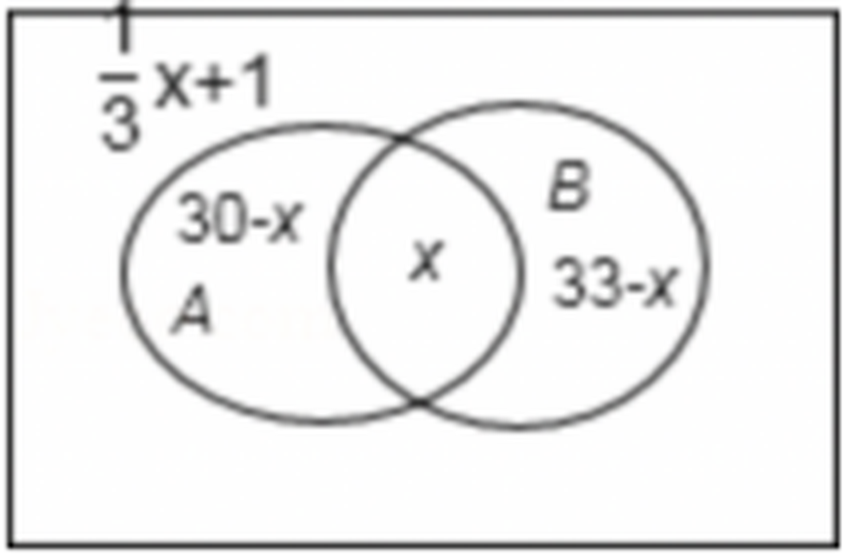
\includegraphics[width=0.30\textwidth]{figures/venn_AB_survey_50.png}
\end{center}

\ans{$21$}

\ifanswer
\solbegin
\step{由题意得赞成 $A$ 的人数 30，赞成 $B$ 的人数为 33，}
\step{设对 $A$、$B$ 都赞成的学生数为 $x$，则对 $A$、$B$ 都不赞成的学生数 $\dfrac{1}{3}x+1$，}
\step{如图得 $x+30-x+33-x+\dfrac{1}{3}x+1=50$，所以 $x=21$.}
\solend

\fi

\item 集合 $S=\{s\mid s=2n+1,n\in\Z\}$，$T=\{t\mid t=4n+1,n\in\Z\}$，则 $S$ \blankline[2.4em] $T$（填“$\subset$”“$\supset$”“$\subseteq$”或“$\supseteq$”）.

\ans{$S\supset T$}

\ifanswer
\solbegin
\step{对于 $S=\{s\mid s=2n+1,n\in\Z\}$ 为奇数，}
\step{而 $T=\{t\mid t=4n+1,n\in\Z\}$ 被 4 整除余 1 的奇数，所以 $S\supset T$.}
\solend

\fi

\item 已知集合 $A=\{x\mid -2<x<4\}$，$B=\{x\mid x^2-3ax+2a^2=0\}$，若 $A\cap B=B$，则实数 $a$ 的取值范围为 \blankline[4.4em].

\ans{$(-1,2)$}

\ifanswer
\solbegin
\step{因为 $A\cap B=B$，所以 $B\subseteq A$，}
\step{①当 $a=0$ 时，方程 $x^2-3ax+2a^2=0$ 的解为 $0$，$B\subseteq A$ 成立；}
\step{②当 $a\neq 0$ 时，方程 $x^2-3ax+2a^2=0$ 的解为 $2a$、$a$，}
\step{则 $-2<2a<4$ 且 $-2<a<4$，解得 $-1<a<2$ 且 $a\neq 0$；}
\step{综上所述，实数 $a$ 的取值范围为 $(-1,2)$.}
\solend

\fi

\item 当一个非空数集 $F$ 满足条件“若 $a$、$b\in F$，则 $a+b$、$a-b$、$ab\in F$，且当 $b\neq 0$ 时，$\dfrac{a}{b}\in F$”时，称 $F$ 为一个数域，以下四个关于数域的命题：

（1）$0$ 是任何数域的元素；（2）若数域 $F$ 有非零元素，则 $2026\in F$；

（3）集合 $P=\{x\mid x=3k,k\in\Z\}$ 为数域；（4）有理数集为数域；

其中，真命题的编号为 \blankline[4.4em]（写出所有真命题的编号）.

\ans{（1）（2）（4）}

\item 对于集合 $M$，定义函数 $f_M(x)=\begin{cases}-1,&x\in M\\ 1,&x\notin M\end{cases}$，对于两个集合 $M$、$N$，定义集合
$M\triangle N=\{x\mid f_M(x)\cdot f_N(x)=-1\}$，已知 $A=\{2,4,6,8,10\},B=\{1,2,4,8,16\}$，用 $|M|$ 表示有限集合 $M$ 中的元素个数，则对于任意集合 $M$，$|M\triangle A|+|M\triangle B|$ 的最小值为 \blankline[2.4em].

% 注：上面分段函数的第二行，原卷印作「1, $x\in M$」（两行都印 $x\in M$），与函数的定义矛盾，
%     本稿按文意订正为 $x\notin M$.
\ans{$4$}

\ifanswer
\solbegin
% 注：下面一行原卷印作「即 $M\triangle N\in\{x\mid x\in M\cup N\}$ 且 $x\in M\cap N$」，「$\in$」当为
%     「$=$」之误，且由 $f_M(x)f_N(x)=-1$ 应对应 $x\notin M\cap N$，本稿一并按文意订正.
\step{由 $M\triangle N$ 的定义得 $f_M(x)\cdot f_N(x)=-1$，}
\step{即 $M\triangle N=\{x\mid x\in M\cup N\text{ 且 }x\notin M\cap N\}$，}
\step{$|M\triangle A|+|M\triangle B|$ 要取得最小值，需满足 $A\cap B\subseteq M\subseteq A\cup B$，}
\step{此时 $|M\triangle A|+|M\triangle B|$ 的最小值为 $4$.}
\solend

\fi

\end{enumerate}

\bigsec{二、选择题}

\begin{enumerate}
\setcounter{enumi}{12}

\item 已知集合 $A=\{x\mid x=3m,m\in\N\}$，$B=\{x\mid x=3m+1,m\in\N\}$，$C=\{x\mid x=3m+2,m\in\N\}$，若 $a\in A$，$b\in B$，$c\in C$，则下列结论中可能成立的是\mbox{（\quad）}

\keepwithprev
A. $2021=a+b+c$\qquad B. $2021=abc$\qquad C. $2021=a+bc$\qquad D. $2021=a(b+c)$

\ans{C}

\ifanswer
\solbegin
\step{由题意设 $a=3m$，$b=3p+1$，$c=3n+2$，$m$、$p$、$n\in\N$，}
\step{则 $a+b+c=3m+3p+1+3n+2=3(m+p+n+1)$，}
\step{故 2021 不是 3 的整数倍，则 A 不可能；}
\step{$abc=3m(3p+1)(3n+2)$，同理 B 不可能；}
\step{$a+bc=3m+(3p+1)(3n+2)=3(m+3pn+2p+n)+2$，$2021=3\times 673+2$，}
\step{如取 $p=n=1$，则 $m=667$，即 $2021=3\times 667+4\times 5$，故 C 成立；}
\step{$a(b+c)=3m(3p+1+3n+2)=9m(p+n+1)$，同 A 可得 D 不可能.}
\step{故选 C.}
\solend

\fi

\item 设 $a$、$b$、$c$ 是实数，$x=a^2-2b+\dfrac{\pi}{3}$，$y=b^2-2c+\dfrac{\pi}{6}$，$z=c^2-2a+\dfrac{\pi}{2}$，则 $x$、$y$、$z$ 中至少有一个值\mbox{（\quad）}

\keepwithprev
A. 大于 $0$\qquad B. 等于 $0$\qquad C. 不大于 $0$\qquad D. 小于 $0$

\ans{A}

\ifanswer
\solbegin
\step{因为 $x+y+z=a^2-2b+\dfrac{\pi}{3}+b^2-2c+\dfrac{\pi}{6}+c^2-2a+\dfrac{\pi}{2}=(a-1)^2+(b-1)^2+(c-1)^2+\pi-3>0$，}
\step{假设 $x$、$y$、$z$ 都不大于 $0$，即 $x\leqslant 0$，$y\leqslant 0$，$z\leqslant 0$，}
\step{由同向不等式的可加性得 $x+y+z\leqslant 0$①，又 $x+y+z>0$ 与①式矛盾.}
\step{所以假设不成立，即原命题的结论 $x$、$y$、$z$ 中至少有一个大于 $0$. 故选 A.}
\solend

\fi

\item 命题“存在一个无理数，它的平方是有理数”的否定是\mbox{（\quad）}

\keepwithprev
A. 任意一个有理数，它的平方是有理数

B. 任意一个无理数，它的平方不是有理数

C. 存在一个有理数，它的平方是有理数

D. 存在一个无理数，它的平方不是有理数

\ans{B}

\ifanswer
\solbegin
\step{否定是任意一个无理数，它的平方不是有理数，故选 B.}
\solend

\fi

\item 设集合 $P_1=\{x\mid x^2+ax+1>0\}$，$P_2=\{x\mid x^2+ax+2>0\}$，$Q_1=\{x\mid x^2+x+b>0\}$，$Q_2=\{x\mid x^2+2x+b>0\}$，其中 $a$、$b\in\R$，下列说法正确的是\mbox{（\quad）}

\keepwithprev
A. 对任意 $a$，$P_1$ 是 $P_2$ 的子集，对任意 $b$，$Q_1$ 不是 $Q_2$ 的子集

B. 对任意 $a$，$P_1$ 是 $P_2$ 的子集，存在 $b$，使得 $Q_1$ 是 $Q_2$ 的子集

C. 对任意 $a$，使得 $P_1$ 不是 $P_2$ 的子集，对任意 $b$，$Q_1$ 不是 $Q_2$ 的子集

D. 对任意 $a$，使得 $P_1$ 不是 $P_2$ 的子集，存在 $b$，使得 $Q_1$ 不是 $Q_2$ 的子集

\ans{B}

\ifanswer
\solbegin
\step{对于集合 $P_1=\{x\mid x^2+ax+1>0\}$，$P_2=\{x\mid x^2+ax+2>0\}$，}
\step{得当 $m\in P_1$，即 $m^2+am+1>0$，得 $m^2+am+2>0$，}
\step{即有 $m\in P_2$，得对任意 $a$，$P_1$ 是 $P_2$ 的子集；}
\step{当 $b=5$ 时，$Q_1=\{x\mid x^2+x+5>0\}=\R$，$Q_2=\{x\mid x^2+2x+5>0\}=\R$，}
\step{得 $Q_1$ 是 $Q_2$ 的子集，故 A 错误，B 正确；}
\step{当 $b=1$ 时，$Q_1=\{x\mid x^2+x+1>0\}=\R$，}
\step{$Q_2=\{x\mid x^2+2x+1>0\}=\{x\mid x\neq -1\text{ 且 }x\in\R\}$，得 $Q_1$ 不是 $Q_2$ 的子集.}
\step{综上，对任意 $a$，$P_1$ 是 $P_2$ 的子集，存在 $b$，使得 $Q_1$ 是 $Q_2$ 的子集，}
\step{故 C 错误，D 错误.}
\step{故选 B.}
\solend

\fi

\end{enumerate}

\bigsec{三、解答题}

\begin{enumerate}
\setcounter{enumi}{16}

\item 已知集合 $A=\{x\mid 0<x-a\leqslant 5\}$，$B=\left\{x\mid -\dfrac{a}{2}<x\leqslant 6\right\}$.

\begin{enumerate}[label=(\arabic*)]
\item 若 $A\subseteq B$，求 $a$ 的取值范围.
\item 集合 $A$ 与 $B$ 能否相等？若能，求出 $a$ 的值，若不能，请说明理由.
\end{enumerate}

\ans{（1）$0\leqslant a\leqslant 1$；（2）不能，$a\in\varnothing$}

\ifanswer
\solbegin
\stepm{（1）}{由于 $A\subseteq B$，所以 $a+5\leqslant 6$，且 $-\dfrac{a}{2}\leqslant a$，解得 $0\leqslant a\leqslant 1$；}
\stepm{（2）}{$A=B$ 时，$a+5=6$，$-\dfrac{a}{2}=a$，解得 $a\in\varnothing$.}
\solend

\fi

\ansspace[6]

\item 已知 $\alpha:2x+m<0$，$\beta:-1<x<3$.

\begin{enumerate}[label=(\arabic*)]
\item 是否存在实数 $m$，使得 $\alpha$ 是 $\beta$ 的充分条件？若存在，求出实数 $m$ 的取值范围；
\item 是否存在实数 $m$，使得 $\alpha$ 是 $\beta$ 的必要条件？若存在，求出实数 $m$ 的取值范围.
\end{enumerate}

\ans{（1）不存在；（2）存在，$m\leqslant -6$}

\ansspace[6]

\item 已知 $\triangle ABC$ 的三边长分别为 $a,b,c$，证明：

\begin{enumerate}[label=(\arabic*)]
\item “$A=90^\circ$”是“关于 $x$ 的方程 $x^2+2ax+b^2=0$ 与 $x^2+2cx-b^2=0$ 有公共实根”的充分条件；
\item “$a=c$”是“关于 $x$ 的方程 $x^2+2ax+b^2=0$ 与 $x^2+2cx-b^2=0$ 没有公共实根”的充分非必要条件.
\end{enumerate}

\ans{（1）略；（2）略}

\ansspace[8]

\item 已知集合 $A$ 包含有 $n(n\in\N^*)$ 个元素，$A^+=\{x+y\mid x\text{、}y\in A\}$.

\begin{enumerate}[label=(\arabic*)]
\item 若 $A=\{0,1,2\}$，写出 $A^+$；
\item % 注：原卷此处印作「写出一个 $A^+$，使得 $A=A^+$」——$A$ 未给定，该问无法作答，
      %     与下方【解析】「取 $A=\{0\}$」不符，本稿按文意订正为「写出一个 $A$」.
      写出一个 $A$，使得 $A=A^+$；
\item 当 $n=4$ 时，是否存在集合 $A$，使得 $A^+=\{2,3,5,6,7,8,10\}$？若存在，求出此时的集合 $A$，若不存在，请说明理由.
\end{enumerate}

\ans{（1）$\{0,1,2,3,4\}$；（2）$A=\{0\}$；（3）不存在}

\ifanswer
\solbegin
\stepm{（1）}{由题意得 $0+0=0$，$0+1=1$，$0+2=2$，$1+1=2$，$1+2=3$，$2+2=4$ 都是 $A^+$ 中的元素，故 $A^+=\{0,1,2,3,4\}$；}
\stepm{（2）}{取 $A=\{0\}$，此时 $A^+=\{x+y\mid x\text{、}y\in A\}=\{0\}$，符合 $A=A^+$；}
\stepm{（3）}{当 $n=4$ 时，不存在集合 $A$，使得 $A^+=\{2,3,5,6,7,8,10\}$，理由如下：}
\step{假设存在 $A=\{a,b,c,d\}$，且 $a<b<c<d$，}
\step{则 $2a<a+b<a+c<b+c<b+d<c+d<2d$，}
\step{故 $2a,a+b,a+c,b+c,b+d,c+d,2d$ 为 $A^+$ 中 7 个不同的元素，}
\step{则 $2a=2$，$a+b=3$，$a+c=5$，$b+c=6$，$b+d=7$，$c+d=8$，$2d=10$，}
\step{解得 $a=1$，$b=2$，$c=4$，$d=5$，}
\step{此时 $c+d=9\in A^+$ 与 $9\notin A^+$ 矛盾，故假设不成立，}
\step{即不存在这样的集合 $A$.}
\solend

\fi

\ansspace[8]

% 压轴题：在其 \item 前先量一下版面，本页剩余高度不足 7cm 就另起一页。
\ansneed{7cm}

\item 已知集合 $A$ 为非空数集，对于集合 $A$，对 $A$ 中任意两个不同元素相加得到的和取绝对值，将这些绝对值重新组成一个新的集合，对于这一过程，我们定义为“自相加”，重新组成的集合叫做“集合 $A$ 的 1 次自相加集合”，再进行 $n-1$ 次“自相加”操作，组成的集合叫做“集合 $A$ 的 $n$ 次自相加集合”. 若集合 $A$ 的任意 $k$ 次自相加集合都不相等，则称集合 $A$ 为“完美自相加集合”，同理，我们可以定义出“$A$ 的 1 次自相减集合”，集合 $A$ 的 1 次自相加集合和 1 次自相减集合分别可表示为：$A^+=\{x\mid x=|a+b|,\ a\text{、}b\in A\}$，$A^-=\{x\mid x=|a-b|,\ a\text{、}b\in A\}$.

\begin{enumerate}[label=(\arabic*)]
\item 已知有两个集合，集合 $B=\{1,2,3,4\}$，集合 $C=\{k\mid k=2n+1,n\in\Z\}$，判断集合 $B$ 和集合 $C$ 是否是完美自相加集合，并说明理由；
\item 对（1）中的集合 $B$ 进行 11 次自相加操作后，求：集合 $B$ 的 11 次自相加集合的元素个数；
\item 若 $0\leqslant n\leqslant 2025$ 且 $n\in\N$，集合 $A=\{x\mid n\leqslant x\leqslant 2025,x\in\N\}$，$A^+\cap A^-=\varnothing$，求：$n$ 的最小值.
\end{enumerate}

\ans{（1）$B$ 是完美自相加集合，$C$ 不是完美自相加集合；（2）$2051$；（3）$675$}

\ifanswer
\solbegin
\stepm{（1）}{$B$ 是完美自相加集合，$C$ 不是完美自相加集合，}
\step{理由如下：因为集合 $B=\{1,2,3,4\}$，所以 $B^+=\{3,4,5,6,7\}$，}
\step{由此可得集合自相加后，}
\step{新的集合中最小的元素为自相加之前的集合中的最小两个元素之和，}
\step{所以显然集合 $B=\{1,2,3,4\}$ 的最小两个元素为 $1$，$2$，}
\step{所以 $B^+$ 中的最小元素为 $1+2=3$，}
\step{同理，2 次自相加后得到的集合中的最小元素是 $3+4=7$.}
\step{依照这样的规律，对集合 $B=\{1,2,3,4\}$ 进行任意次自相加操作后，}
\step{最小值总在变大，故不可能有相等集合，所以 $B$ 是完美自相加集合；}
\step{因为集合 $C=\{k\mid k=2n+1,n\in\Z\}$ 表示所有奇数构成的集合，}
\step{任何两个奇数相加的和都是偶数，}
\step{所以 $C^+=\{k\mid k=2n,n\in\Z\}$ 为所有偶数构成集合；}
\step{所以对 $C^+=\{k\mid k=2n,n\in\Z\}$ 再进行一次自相加操作，}
\step{因为任意两个偶数相加的和还是偶数，}
\step{所以后面集合不管进行多少次相加都与 $C^+=\{k\mid k=2n,n\in\Z\}$ 相同；}
\step{故 $C$ 不是完美自相加集合.}
\stepm{（2）}{由自相加性质得，对于集合 $B=\{1,2,3,4\}$，进行一次自相加，}
\step{得到集合的最小值必然是原来集合的两个最小元素值之和，}
\step{得到的最大值必然为原来集合的两个最大元素值之和，}
\step{且中间必然是连续的整数元素；}
\step{所以对集合 $B=\{1,2,3,4\}$ 进行 1 次自相加之后，}
\step{得到的集合最小两个元素为 $3$，$4$，最大的两个元素为 $6$，$7$；}
\step{进行第 2 次自相加，得到的集合最小两个元素为 $7$，$8$，}
\step{最大的两个元素为 $12$，$13$；}
\step{进行第 3 次自相加，得到的集合最小两个元素为 $15$，$16$，}
\step{最大的两个元素为 $24$，$25$；}
\step{进行第 4 次自相加，得到的集合最小两个元素为 $31$，$32$，}
\step{最大的两个元素为 $48$，$49$；}
\step{进行第 5 次自相加，得到的集合最小两个元素为 $63$，$64$，}
\step{最大的两个元素为 $96$，$97$；}
\step{进行第 6 次自相加，得到的集合最小两个元素为 $127$，$128$，}
\step{最大的两个元素为 $192$，$193$；}
\step{进行第 7 次自相加，得到的集合最小两个元素为 $255$，$256$，}
\step{最大的两个元素为 $384$，$385$；}
\step{进行第 8 次自相加，得到的集合最小两个元素为 $511$，$512$，}
\step{最大的两个元素为 $768$，$769$；}
\step{进行第 9 次自相加，得到的集合最小两个元素为 $1023$，$1024$，}
\step{最大的两个元素为 $1536$，$1537$；}
\step{进行第 10 次自相加，得到的集合最小两个元素为 $2047$，$2048$，}
\step{最大的两个元素为 $3072$，$3073$；}
\step{进行第 11 次自相加，得到的集合最小两个元素为 $4095$，$4096$，}
\step{最大的两个元素为 $6144$，$6145$；}
\step{因为集合 $B$ 的 $n$ 次自相加集合中的元素都是连续的整数，}
\step{所以集合 $B$ 进行 11 次自相加操作后的元素个数为 $6145-4095+1=2051$.}
\stepm{（3）}{因为 $0\leqslant n\leqslant 2025$ 且 $n\in\N$，集合 $A=\{x\mid n\leqslant x\leqslant 2025,x\in\N\}$，}
\step{所以 $A^+=\{x\mid 2n+1\leqslant x\leqslant 4049,x\in\N\}$，}
\step{$A^-=\{x\mid 1\leqslant x\leqslant 2025-n,x\in\N\}$，}
\step{要使 $A^+\cap A^-=\varnothing$，须使 $2n+1>2025-n$，所以 $n>\dfrac{2024}{3}=674\dfrac{2}{3}$，}
\step{又 $n\in\N$，故 $n$ 的最小值为 $675$.}
\solend

\fi

% 压轴题：其后已无内容，故作答区全用可丢弃胶水（\ansspace*）。
\ansspace*[12]

\end{enumerate}

\end{document}
"
%
% 原始材料是微信公众号图文（公众号「魔都数学加油站」），正文为 10 张 PNG 页（1080×1527）。
% 原文本身就是一份**讲评版**——题目下方直接印出【答案】或【解析】，选择题的答案印在解析末句
% 「故选 X」里。试题文字、答案与解析均照原卷录入（订正处见下），卷面上的粉色斜水印
% 「魔都数学加油站」属水印，未录入。
%
% 与原卷的排版差异（均已在 README「说明」中交代）：
%   ① 原文自**第 3 题**起（第 1、2 题未在该文中发布），故本稿题号亦自 3 起；
%   ② 原卷本就印有「一、填空题」「二、选择题」「三、解答题」三节标题（分别在原图 00/02/04.png
%      上，逐页核对过），本稿照原卷分节，只把标题改排成全稿统一的「大节标题」样式；
%   ③ 原卷填空、选择的答案直接印在题目下方（选择题只在解析末句「故选 X」中给出），本稿统一改为
%      试卷版隐去、答案版以【答案】给出，选择题的括注一律改排「\mbox{（\quad）}」并把答案移到选项之后，
%      使两版彻底分离；
%   ④ 原卷的集合符号大小写混用：第 3 题题干的实数集印成**粗体** $\mathbf{R}$，第 16 题题干与
%      第 16 题解析的印成正体 $R$；自然数集 $N$、整数集 $Z$ 一律正体。本稿按全稿惯例统一写作
%      $\R$、$\N$、$\Z$；
%   ⑤ 原卷未印副标题，本稿按全稿惯例补出副标题「集合与常用逻辑用语」；
%   ⑥ 原卷解答题子问编号为「（1）（2）」，本稿用嵌套 enumerate 排成同一形态；原卷第 15 题的
%      D 选项因原页翻页被截到下一页首页，本稿自然连排；
%   ⑦ 原卷解答题未留作答空间（讲评稿通篇是答案），本稿逐题补出书写留白，仅试卷版显示；
%   ⑧ 第 21 题题干里 $A^+$、$A^-$ 的定义含绝对值号（原卷作 $\{x\mid x=|a+b|,\ a\text{、}b\in A\}$
%      与 $\{x\mid x=|a-b|,\ a\text{、}b\in A\}$），本稿照原卷录入；2026-09-15 回原图逐处放大复核
%      时发现曾漏抄两处绝对值号、并把分隔逗号误写成 $\mid$，已按原卷订正（见 README 专记）。
%
% 原卷笔误三处（均已放大到能看清字形后核对，本稿按文意订正，并在 README 中写明原委）：
%   ① 第 12 题题干的分段函数 $f_M(x)$ 原卷两行都印作「$x\in M$」（$-1$ 与 $1$ 都取在 $M$ 上），
%      与「函数」的定义直接矛盾（$M$ 上无法同时取两个值），按文意订正第二行为 $x\notin M$；
%   ② 第 12 题【解析】首行原卷印「即 $M\triangle N\in\{x\mid x\in M\cup N\}$ 且 $x\in M\cap N$」，
%      其中「$\in$」当为「$=$」之误；且由 $f_M(x)f_N(x)=-1$ 应对应 $x\notin M\cap N$（原卷印作
%      $x\in M\cap N$，与上一行刚写出的对称差的定义相矛盾），本稿一并订正；
%   ③ 第 20 题(2)原卷印「写出一个 $A^+$，使得 $A=A^+$」——$A$ 未给定，该问无法作答，与紧接的
%      【解析】「取 $A=\{0\}$，此时 $A^+=\{0\}$，符合 $A=A^+$」不符，本稿按文意订正为
%      「写出一个 $A$，使得 $A=A^+$」.
%
% 原卷存疑一处（无法确证原意，本稿照抄原卷、未改）：
%   ① 第 5 题 ④ 原卷题干印 $S=\{x\mid |x|\leqslant\sqrt{3},x\in N\}$（该字母与 ③ 中的 $Z$
%      字形明显不同，$Z$ 有上下两横，已放大比对确认），而【解析】印「因为 $S=\{-1,0,1\}$」——
%      按 $x\in N$ 应为 $S=\{0,1\}$（或 $\{1\}$），题干与解析的口径不一致；但无论取哪一口径，
%      ④ 都是 $M$ 的子集、本题结论（填④）不变，故题干与解析均照抄原卷，未改。

\documentclass[a4paper,11pt]{article}
\usepackage{common}

\begin{document}

\examtitlest{2026--2027 年七宝中学高一上周末作业 2}{集合与常用逻辑用语}

\bigsec{一、填空题}

\begin{enumerate}
\setcounter{enumi}{2}

\item 已知 $a,x\in\R$，则“$x\in\{-a,a\}$”是“$|x|=a$”的 \blankline[4.4em] 条件.

\ans{必要不充分}

\item 设全集为 $U$，$A\subseteq U$，$B\subseteq U$，则“$A\subset B$”是“$\overline{B}\subset\overline{A}$”的 \blankline[4.4em] 条件.

\ans{充要}

\item 已知集合 $M=\{x\mid -\sqrt{5}<x<\sqrt{3},x\in\Z\}$，则下列集合是集合 $M$ 的子集的是 \blankline[4.4em]（填序号）.

① $P=\{-3,0,1\}$；② $Q=\{-1,0,1,2\}$；③ $R=\{y\mid -\pi<y<-1,y\in\Z\}$；

④ $S=\{x\mid |x|\leqslant\sqrt{3},x\in\N\}$.

\ans{④}

\ifanswer
\solbegin
\step{由已知得集合 $M=\{-2,-1,0,1\}$，}
\step{所以由子集的定义得选项①错误，②错误，}
\step{因为 $R=\{-3,-2\}$，所以集合 $R$ 不表示集合 $M$ 的子集，③错误，}
\step{因为 $S=\{-1,0,1\}$，所以是集合 $M$ 的子集，故正确.}
\step{故是集合 $M$ 的子集的是④.}
\solend

\fi

\item 已知 $x\in\R$，用反证法证明命题“若 $x^2-7x+10<0$，则 $2<x<5$”时，应该假设 \blankline[5em].

\ans{$x\leqslant 2$ 或 $x\geqslant 5$}

\item 设 $a_1,b_1,c_1,a_2,b_2,c_2$ 均为非零实数，方程 $a_1x^2+b_1x+c_1=0$ 和 $a_2x^2+b_2x+c_2=0$ 的解集分别为 $M$ 和 $N$，那么“$\dfrac{a_1}{a_2}=\dfrac{b_1}{b_2}=\dfrac{c_1}{c_2}$”是“$M=N$”的 \blankline[4.4em] 条件.

（填“充分非必要”、“必要非充分”、“充要”、或“既非充分又非必要”）

\ans{充分非必要}

\ifanswer
\solbegin
\step{$\dfrac{a_1}{a_2}=\dfrac{b_1}{b_2}=\dfrac{c_1}{c_2}$ 能推出 $M=N$，}
\step{若 $M=N=\varnothing$ 推不出 $\dfrac{a_1}{a_2}=\dfrac{b_1}{b_2}=\dfrac{c_1}{c_2}$，}
\step{所以“$\dfrac{a_1}{a_2}=\dfrac{b_1}{b_2}=\dfrac{c_1}{c_2}$”是“$M=N$”的“充分非必要”条件.}
\solend

\fi

\item 向 50 名学生调查对 $A$、$B$ 两事件的态度，有如下结果赞成 $A$ 的人数是全体的五分之三，其余的不赞成，赞成 $B$ 的比赞成 $A$ 的多 3 人，其余的不赞成；另外，对 $A$、$B$ 都不赞成的学生数比对 $A$、$B$ 都赞成的学生数的三分之一多 1 人. 则对 $A$、$B$ 都赞成的学生有 \blankline[2.4em] 人.

\begin{center}
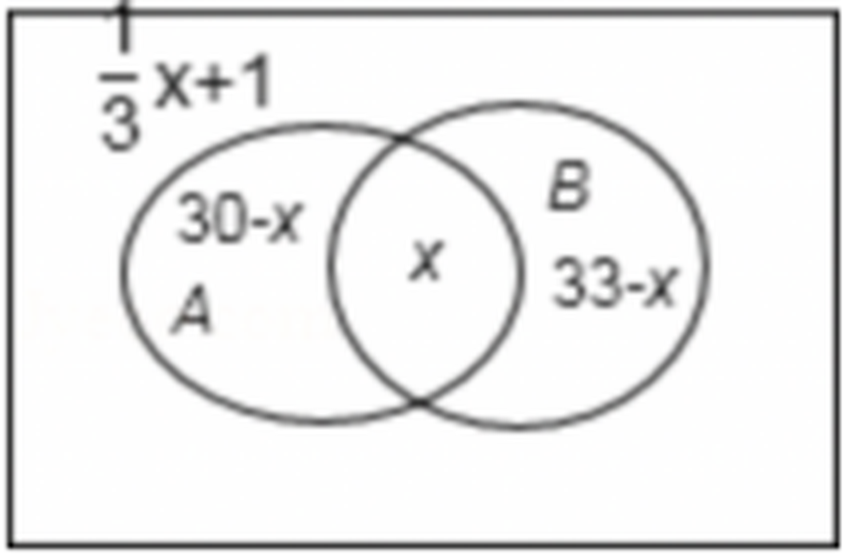
\includegraphics[width=0.30\textwidth]{figures/venn_AB_survey_50.png}
\end{center}

\ans{$21$}

\ifanswer
\solbegin
\step{由题意得赞成 $A$ 的人数 30，赞成 $B$ 的人数为 33，}
\step{设对 $A$、$B$ 都赞成的学生数为 $x$，则对 $A$、$B$ 都不赞成的学生数 $\dfrac{1}{3}x+1$，}
\step{如图得 $x+30-x+33-x+\dfrac{1}{3}x+1=50$，所以 $x=21$.}
\solend

\fi

\item 集合 $S=\{s\mid s=2n+1,n\in\Z\}$，$T=\{t\mid t=4n+1,n\in\Z\}$，则 $S$ \blankline[2.4em] $T$（填“$\subset$”“$\supset$”“$\subseteq$”或“$\supseteq$”）.

\ans{$S\supset T$}

\ifanswer
\solbegin
\step{对于 $S=\{s\mid s=2n+1,n\in\Z\}$ 为奇数，}
\step{而 $T=\{t\mid t=4n+1,n\in\Z\}$ 被 4 整除余 1 的奇数，所以 $S\supset T$.}
\solend

\fi

\item 已知集合 $A=\{x\mid -2<x<4\}$，$B=\{x\mid x^2-3ax+2a^2=0\}$，若 $A\cap B=B$，则实数 $a$ 的取值范围为 \blankline[4.4em].

\ans{$(-1,2)$}

\ifanswer
\solbegin
\step{因为 $A\cap B=B$，所以 $B\subseteq A$，}
\step{①当 $a=0$ 时，方程 $x^2-3ax+2a^2=0$ 的解为 $0$，$B\subseteq A$ 成立；}
\step{②当 $a\neq 0$ 时，方程 $x^2-3ax+2a^2=0$ 的解为 $2a$、$a$，}
\step{则 $-2<2a<4$ 且 $-2<a<4$，解得 $-1<a<2$ 且 $a\neq 0$；}
\step{综上所述，实数 $a$ 的取值范围为 $(-1,2)$.}
\solend

\fi

\item 当一个非空数集 $F$ 满足条件“若 $a$、$b\in F$，则 $a+b$、$a-b$、$ab\in F$，且当 $b\neq 0$ 时，$\dfrac{a}{b}\in F$”时，称 $F$ 为一个数域，以下四个关于数域的命题：

（1）$0$ 是任何数域的元素；（2）若数域 $F$ 有非零元素，则 $2026\in F$；

（3）集合 $P=\{x\mid x=3k,k\in\Z\}$ 为数域；（4）有理数集为数域；

其中，真命题的编号为 \blankline[4.4em]（写出所有真命题的编号）.

\ans{（1）（2）（4）}

\item 对于集合 $M$，定义函数 $f_M(x)=\begin{cases}-1,&x\in M\\ 1,&x\notin M\end{cases}$，对于两个集合 $M$、$N$，定义集合
$M\triangle N=\{x\mid f_M(x)\cdot f_N(x)=-1\}$，已知 $A=\{2,4,6,8,10\},B=\{1,2,4,8,16\}$，用 $|M|$ 表示有限集合 $M$ 中的元素个数，则对于任意集合 $M$，$|M\triangle A|+|M\triangle B|$ 的最小值为 \blankline[2.4em].

% 注：上面分段函数的第二行，原卷印作「1, $x\in M$」（两行都印 $x\in M$），与函数的定义矛盾，
%     本稿按文意订正为 $x\notin M$.
\ans{$4$}

\ifanswer
\solbegin
% 注：下面一行原卷印作「即 $M\triangle N\in\{x\mid x\in M\cup N\}$ 且 $x\in M\cap N$」，「$\in$」当为
%     「$=$」之误，且由 $f_M(x)f_N(x)=-1$ 应对应 $x\notin M\cap N$，本稿一并按文意订正.
\step{由 $M\triangle N$ 的定义得 $f_M(x)\cdot f_N(x)=-1$，}
\step{即 $M\triangle N=\{x\mid x\in M\cup N\text{ 且 }x\notin M\cap N\}$，}
\step{$|M\triangle A|+|M\triangle B|$ 要取得最小值，需满足 $A\cap B\subseteq M\subseteq A\cup B$，}
\step{此时 $|M\triangle A|+|M\triangle B|$ 的最小值为 $4$.}
\solend

\fi

\end{enumerate}

\bigsec{二、选择题}

\begin{enumerate}
\setcounter{enumi}{12}

\item 已知集合 $A=\{x\mid x=3m,m\in\N\}$，$B=\{x\mid x=3m+1,m\in\N\}$，$C=\{x\mid x=3m+2,m\in\N\}$，若 $a\in A$，$b\in B$，$c\in C$，则下列结论中可能成立的是\mbox{（\quad）}

\keepwithprev
A. $2021=a+b+c$\qquad B. $2021=abc$\qquad C. $2021=a+bc$\qquad D. $2021=a(b+c)$

\ans{C}

\ifanswer
\solbegin
\step{由题意设 $a=3m$，$b=3p+1$，$c=3n+2$，$m$、$p$、$n\in\N$，}
\step{则 $a+b+c=3m+3p+1+3n+2=3(m+p+n+1)$，}
\step{故 2021 不是 3 的整数倍，则 A 不可能；}
\step{$abc=3m(3p+1)(3n+2)$，同理 B 不可能；}
\step{$a+bc=3m+(3p+1)(3n+2)=3(m+3pn+2p+n)+2$，$2021=3\times 673+2$，}
\step{如取 $p=n=1$，则 $m=667$，即 $2021=3\times 667+4\times 5$，故 C 成立；}
\step{$a(b+c)=3m(3p+1+3n+2)=9m(p+n+1)$，同 A 可得 D 不可能.}
\step{故选 C.}
\solend

\fi

\item 设 $a$、$b$、$c$ 是实数，$x=a^2-2b+\dfrac{\pi}{3}$，$y=b^2-2c+\dfrac{\pi}{6}$，$z=c^2-2a+\dfrac{\pi}{2}$，则 $x$、$y$、$z$ 中至少有一个值\mbox{（\quad）}

\keepwithprev
A. 大于 $0$\qquad B. 等于 $0$\qquad C. 不大于 $0$\qquad D. 小于 $0$

\ans{A}

\ifanswer
\solbegin
\step{因为 $x+y+z=a^2-2b+\dfrac{\pi}{3}+b^2-2c+\dfrac{\pi}{6}+c^2-2a+\dfrac{\pi}{2}=(a-1)^2+(b-1)^2+(c-1)^2+\pi-3>0$，}
\step{假设 $x$、$y$、$z$ 都不大于 $0$，即 $x\leqslant 0$，$y\leqslant 0$，$z\leqslant 0$，}
\step{由同向不等式的可加性得 $x+y+z\leqslant 0$①，又 $x+y+z>0$ 与①式矛盾.}
\step{所以假设不成立，即原命题的结论 $x$、$y$、$z$ 中至少有一个大于 $0$. 故选 A.}
\solend

\fi

\item 命题“存在一个无理数，它的平方是有理数”的否定是\mbox{（\quad）}

\keepwithprev
A. 任意一个有理数，它的平方是有理数

B. 任意一个无理数，它的平方不是有理数

C. 存在一个有理数，它的平方是有理数

D. 存在一个无理数，它的平方不是有理数

\ans{B}

\ifanswer
\solbegin
\step{否定是任意一个无理数，它的平方不是有理数，故选 B.}
\solend

\fi

\item 设集合 $P_1=\{x\mid x^2+ax+1>0\}$，$P_2=\{x\mid x^2+ax+2>0\}$，$Q_1=\{x\mid x^2+x+b>0\}$，$Q_2=\{x\mid x^2+2x+b>0\}$，其中 $a$、$b\in\R$，下列说法正确的是\mbox{（\quad）}

\keepwithprev
A. 对任意 $a$，$P_1$ 是 $P_2$ 的子集，对任意 $b$，$Q_1$ 不是 $Q_2$ 的子集

B. 对任意 $a$，$P_1$ 是 $P_2$ 的子集，存在 $b$，使得 $Q_1$ 是 $Q_2$ 的子集

C. 对任意 $a$，使得 $P_1$ 不是 $P_2$ 的子集，对任意 $b$，$Q_1$ 不是 $Q_2$ 的子集

D. 对任意 $a$，使得 $P_1$ 不是 $P_2$ 的子集，存在 $b$，使得 $Q_1$ 不是 $Q_2$ 的子集

\ans{B}

\ifanswer
\solbegin
\step{对于集合 $P_1=\{x\mid x^2+ax+1>0\}$，$P_2=\{x\mid x^2+ax+2>0\}$，}
\step{得当 $m\in P_1$，即 $m^2+am+1>0$，得 $m^2+am+2>0$，}
\step{即有 $m\in P_2$，得对任意 $a$，$P_1$ 是 $P_2$ 的子集；}
\step{当 $b=5$ 时，$Q_1=\{x\mid x^2+x+5>0\}=\R$，$Q_2=\{x\mid x^2+2x+5>0\}=\R$，}
\step{得 $Q_1$ 是 $Q_2$ 的子集，故 A 错误，B 正确；}
\step{当 $b=1$ 时，$Q_1=\{x\mid x^2+x+1>0\}=\R$，}
\step{$Q_2=\{x\mid x^2+2x+1>0\}=\{x\mid x\neq -1\text{ 且 }x\in\R\}$，得 $Q_1$ 不是 $Q_2$ 的子集.}
\step{综上，对任意 $a$，$P_1$ 是 $P_2$ 的子集，存在 $b$，使得 $Q_1$ 是 $Q_2$ 的子集，}
\step{故 C 错误，D 错误.}
\step{故选 B.}
\solend

\fi

\end{enumerate}

\bigsec{三、解答题}

\begin{enumerate}
\setcounter{enumi}{16}

\item 已知集合 $A=\{x\mid 0<x-a\leqslant 5\}$，$B=\left\{x\mid -\dfrac{a}{2}<x\leqslant 6\right\}$.

\begin{enumerate}[label=(\arabic*)]
\item 若 $A\subseteq B$，求 $a$ 的取值范围.
\item 集合 $A$ 与 $B$ 能否相等？若能，求出 $a$ 的值，若不能，请说明理由.
\end{enumerate}

\ans{（1）$0\leqslant a\leqslant 1$；（2）不能，$a\in\varnothing$}

\ifanswer
\solbegin
\stepm{（1）}{由于 $A\subseteq B$，所以 $a+5\leqslant 6$，且 $-\dfrac{a}{2}\leqslant a$，解得 $0\leqslant a\leqslant 1$；}
\stepm{（2）}{$A=B$ 时，$a+5=6$，$-\dfrac{a}{2}=a$，解得 $a\in\varnothing$.}
\solend

\fi

\ansspace[6]

\item 已知 $\alpha:2x+m<0$，$\beta:-1<x<3$.

\begin{enumerate}[label=(\arabic*)]
\item 是否存在实数 $m$，使得 $\alpha$ 是 $\beta$ 的充分条件？若存在，求出实数 $m$ 的取值范围；
\item 是否存在实数 $m$，使得 $\alpha$ 是 $\beta$ 的必要条件？若存在，求出实数 $m$ 的取值范围.
\end{enumerate}

\ans{（1）不存在；（2）存在，$m\leqslant -6$}

\ansspace[6]

\item 已知 $\triangle ABC$ 的三边长分别为 $a,b,c$，证明：

\begin{enumerate}[label=(\arabic*)]
\item “$A=90^\circ$”是“关于 $x$ 的方程 $x^2+2ax+b^2=0$ 与 $x^2+2cx-b^2=0$ 有公共实根”的充分条件；
\item “$a=c$”是“关于 $x$ 的方程 $x^2+2ax+b^2=0$ 与 $x^2+2cx-b^2=0$ 没有公共实根”的充分非必要条件.
\end{enumerate}

\ans{（1）略；（2）略}

\ansspace[8]

\item 已知集合 $A$ 包含有 $n(n\in\N^*)$ 个元素，$A^+=\{x+y\mid x\text{、}y\in A\}$.

\begin{enumerate}[label=(\arabic*)]
\item 若 $A=\{0,1,2\}$，写出 $A^+$；
\item % 注：原卷此处印作「写出一个 $A^+$，使得 $A=A^+$」——$A$ 未给定，该问无法作答，
      %     与下方【解析】「取 $A=\{0\}$」不符，本稿按文意订正为「写出一个 $A$」.
      写出一个 $A$，使得 $A=A^+$；
\item 当 $n=4$ 时，是否存在集合 $A$，使得 $A^+=\{2,3,5,6,7,8,10\}$？若存在，求出此时的集合 $A$，若不存在，请说明理由.
\end{enumerate}

\ans{（1）$\{0,1,2,3,4\}$；（2）$A=\{0\}$；（3）不存在}

\ifanswer
\solbegin
\stepm{（1）}{由题意得 $0+0=0$，$0+1=1$，$0+2=2$，$1+1=2$，$1+2=3$，$2+2=4$ 都是 $A^+$ 中的元素，故 $A^+=\{0,1,2,3,4\}$；}
\stepm{（2）}{取 $A=\{0\}$，此时 $A^+=\{x+y\mid x\text{、}y\in A\}=\{0\}$，符合 $A=A^+$；}
\stepm{（3）}{当 $n=4$ 时，不存在集合 $A$，使得 $A^+=\{2,3,5,6,7,8,10\}$，理由如下：}
\step{假设存在 $A=\{a,b,c,d\}$，且 $a<b<c<d$，}
\step{则 $2a<a+b<a+c<b+c<b+d<c+d<2d$，}
\step{故 $2a,a+b,a+c,b+c,b+d,c+d,2d$ 为 $A^+$ 中 7 个不同的元素，}
\step{则 $2a=2$，$a+b=3$，$a+c=5$，$b+c=6$，$b+d=7$，$c+d=8$，$2d=10$，}
\step{解得 $a=1$，$b=2$，$c=4$，$d=5$，}
\step{此时 $c+d=9\in A^+$ 与 $9\notin A^+$ 矛盾，故假设不成立，}
\step{即不存在这样的集合 $A$.}
\solend

\fi

\ansspace[8]

% 压轴题：在其 \item 前先量一下版面，本页剩余高度不足 7cm 就另起一页。
\ansneed{7cm}

\item 已知集合 $A$ 为非空数集，对于集合 $A$，对 $A$ 中任意两个不同元素相加得到的和取绝对值，将这些绝对值重新组成一个新的集合，对于这一过程，我们定义为“自相加”，重新组成的集合叫做“集合 $A$ 的 1 次自相加集合”，再进行 $n-1$ 次“自相加”操作，组成的集合叫做“集合 $A$ 的 $n$ 次自相加集合”. 若集合 $A$ 的任意 $k$ 次自相加集合都不相等，则称集合 $A$ 为“完美自相加集合”，同理，我们可以定义出“$A$ 的 1 次自相减集合”，集合 $A$ 的 1 次自相加集合和 1 次自相减集合分别可表示为：$A^+=\{x\mid x=|a+b|,\ a\text{、}b\in A\}$，$A^-=\{x\mid x=|a-b|,\ a\text{、}b\in A\}$.

\begin{enumerate}[label=(\arabic*)]
\item 已知有两个集合，集合 $B=\{1,2,3,4\}$，集合 $C=\{k\mid k=2n+1,n\in\Z\}$，判断集合 $B$ 和集合 $C$ 是否是完美自相加集合，并说明理由；
\item 对（1）中的集合 $B$ 进行 11 次自相加操作后，求：集合 $B$ 的 11 次自相加集合的元素个数；
\item 若 $0\leqslant n\leqslant 2025$ 且 $n\in\N$，集合 $A=\{x\mid n\leqslant x\leqslant 2025,x\in\N\}$，$A^+\cap A^-=\varnothing$，求：$n$ 的最小值.
\end{enumerate}

\ans{（1）$B$ 是完美自相加集合，$C$ 不是完美自相加集合；（2）$2051$；（3）$675$}

\ifanswer
\solbegin
\stepm{（1）}{$B$ 是完美自相加集合，$C$ 不是完美自相加集合，}
\step{理由如下：因为集合 $B=\{1,2,3,4\}$，所以 $B^+=\{3,4,5,6,7\}$，}
\step{由此可得集合自相加后，}
\step{新的集合中最小的元素为自相加之前的集合中的最小两个元素之和，}
\step{所以显然集合 $B=\{1,2,3,4\}$ 的最小两个元素为 $1$，$2$，}
\step{所以 $B^+$ 中的最小元素为 $1+2=3$，}
\step{同理，2 次自相加后得到的集合中的最小元素是 $3+4=7$.}
\step{依照这样的规律，对集合 $B=\{1,2,3,4\}$ 进行任意次自相加操作后，}
\step{最小值总在变大，故不可能有相等集合，所以 $B$ 是完美自相加集合；}
\step{因为集合 $C=\{k\mid k=2n+1,n\in\Z\}$ 表示所有奇数构成的集合，}
\step{任何两个奇数相加的和都是偶数，}
\step{所以 $C^+=\{k\mid k=2n,n\in\Z\}$ 为所有偶数构成集合；}
\step{所以对 $C^+=\{k\mid k=2n,n\in\Z\}$ 再进行一次自相加操作，}
\step{因为任意两个偶数相加的和还是偶数，}
\step{所以后面集合不管进行多少次相加都与 $C^+=\{k\mid k=2n,n\in\Z\}$ 相同；}
\step{故 $C$ 不是完美自相加集合.}
\stepm{（2）}{由自相加性质得，对于集合 $B=\{1,2,3,4\}$，进行一次自相加，}
\step{得到集合的最小值必然是原来集合的两个最小元素值之和，}
\step{得到的最大值必然为原来集合的两个最大元素值之和，}
\step{且中间必然是连续的整数元素；}
\step{所以对集合 $B=\{1,2,3,4\}$ 进行 1 次自相加之后，}
\step{得到的集合最小两个元素为 $3$，$4$，最大的两个元素为 $6$，$7$；}
\step{进行第 2 次自相加，得到的集合最小两个元素为 $7$，$8$，}
\step{最大的两个元素为 $12$，$13$；}
\step{进行第 3 次自相加，得到的集合最小两个元素为 $15$，$16$，}
\step{最大的两个元素为 $24$，$25$；}
\step{进行第 4 次自相加，得到的集合最小两个元素为 $31$，$32$，}
\step{最大的两个元素为 $48$，$49$；}
\step{进行第 5 次自相加，得到的集合最小两个元素为 $63$，$64$，}
\step{最大的两个元素为 $96$，$97$；}
\step{进行第 6 次自相加，得到的集合最小两个元素为 $127$，$128$，}
\step{最大的两个元素为 $192$，$193$；}
\step{进行第 7 次自相加，得到的集合最小两个元素为 $255$，$256$，}
\step{最大的两个元素为 $384$，$385$；}
\step{进行第 8 次自相加，得到的集合最小两个元素为 $511$，$512$，}
\step{最大的两个元素为 $768$，$769$；}
\step{进行第 9 次自相加，得到的集合最小两个元素为 $1023$，$1024$，}
\step{最大的两个元素为 $1536$，$1537$；}
\step{进行第 10 次自相加，得到的集合最小两个元素为 $2047$，$2048$，}
\step{最大的两个元素为 $3072$，$3073$；}
\step{进行第 11 次自相加，得到的集合最小两个元素为 $4095$，$4096$，}
\step{最大的两个元素为 $6144$，$6145$；}
\step{因为集合 $B$ 的 $n$ 次自相加集合中的元素都是连续的整数，}
\step{所以集合 $B$ 进行 11 次自相加操作后的元素个数为 $6145-4095+1=2051$.}
\stepm{（3）}{因为 $0\leqslant n\leqslant 2025$ 且 $n\in\N$，集合 $A=\{x\mid n\leqslant x\leqslant 2025,x\in\N\}$，}
\step{所以 $A^+=\{x\mid 2n+1\leqslant x\leqslant 4049,x\in\N\}$，}
\step{$A^-=\{x\mid 1\leqslant x\leqslant 2025-n,x\in\N\}$，}
\step{要使 $A^+\cap A^-=\varnothing$，须使 $2n+1>2025-n$，所以 $n>\dfrac{2024}{3}=674\dfrac{2}{3}$，}
\step{又 $n\in\N$，故 $n$ 的最小值为 $675$.}
\solend

\fi

% 压轴题：其后已无内容，故作答区全用可丢弃胶水（\ansspace*）。
\ansspace*[12]

\end{enumerate}

\end{document}
"
%
% 原始材料是微信公众号图文（公众号「魔都数学加油站」），正文为 10 张 PNG 页（1080×1527）。
% 原文本身就是一份**讲评版**——题目下方直接印出【答案】或【解析】，选择题的答案印在解析末句
% 「故选 X」里。试题文字、答案与解析均照原卷录入（订正处见下），卷面上的粉色斜水印
% 「魔都数学加油站」属水印，未录入。
%
% 与原卷的排版差异（均已在 README「说明」中交代）：
%   ① 原文自**第 3 题**起（第 1、2 题未在该文中发布），故本稿题号亦自 3 起；
%   ② 原卷本就印有「一、填空题」「二、选择题」「三、解答题」三节标题（分别在原图 00/02/04.png
%      上，逐页核对过），本稿照原卷分节，只把标题改排成全稿统一的「大节标题」样式；
%   ③ 原卷填空、选择的答案直接印在题目下方（选择题只在解析末句「故选 X」中给出），本稿统一改为
%      试卷版隐去、答案版以【答案】给出，选择题的括注一律改排「\mbox{（\quad）}」并把答案移到选项之后，
%      使两版彻底分离；
%   ④ 原卷的集合符号大小写混用：第 3 题题干的实数集印成**粗体** $\mathbf{R}$，第 16 题题干与
%      第 16 题解析的印成正体 $R$；自然数集 $N$、整数集 $Z$ 一律正体。本稿按全稿惯例统一写作
%      $\R$、$\N$、$\Z$；
%   ⑤ 原卷未印副标题，本稿按全稿惯例补出副标题「集合与常用逻辑用语」；
%   ⑥ 原卷解答题子问编号为「（1）（2）」，本稿用嵌套 enumerate 排成同一形态；原卷第 15 题的
%      D 选项因原页翻页被截到下一页首页，本稿自然连排；
%   ⑦ 原卷解答题未留作答空间（讲评稿通篇是答案），本稿逐题补出书写留白，仅试卷版显示；
%   ⑧ 第 21 题题干里 $A^+$、$A^-$ 的定义含绝对值号（原卷作 $\{x\mid x=|a+b|,\ a\text{、}b\in A\}$
%      与 $\{x\mid x=|a-b|,\ a\text{、}b\in A\}$），本稿照原卷录入；2026-09-15 回原图逐处放大复核
%      时发现曾漏抄两处绝对值号、并把分隔逗号误写成 $\mid$，已按原卷订正（见 README 专记）。
%
% 原卷笔误三处（均已放大到能看清字形后核对，本稿按文意订正，并在 README 中写明原委）：
%   ① 第 12 题题干的分段函数 $f_M(x)$ 原卷两行都印作「$x\in M$」（$-1$ 与 $1$ 都取在 $M$ 上），
%      与「函数」的定义直接矛盾（$M$ 上无法同时取两个值），按文意订正第二行为 $x\notin M$；
%   ② 第 12 题【解析】首行原卷印「即 $M\triangle N\in\{x\mid x\in M\cup N\}$ 且 $x\in M\cap N$」，
%      其中「$\in$」当为「$=$」之误；且由 $f_M(x)f_N(x)=-1$ 应对应 $x\notin M\cap N$（原卷印作
%      $x\in M\cap N$，与上一行刚写出的对称差的定义相矛盾），本稿一并订正；
%   ③ 第 20 题(2)原卷印「写出一个 $A^+$，使得 $A=A^+$」——$A$ 未给定，该问无法作答，与紧接的
%      【解析】「取 $A=\{0\}$，此时 $A^+=\{0\}$，符合 $A=A^+$」不符，本稿按文意订正为
%      「写出一个 $A$，使得 $A=A^+$」.
%
% 原卷存疑一处（无法确证原意，本稿照抄原卷、未改）：
%   ① 第 5 题 ④ 原卷题干印 $S=\{x\mid |x|\leqslant\sqrt{3},x\in N\}$（该字母与 ③ 中的 $Z$
%      字形明显不同，$Z$ 有上下两横，已放大比对确认），而【解析】印「因为 $S=\{-1,0,1\}$」——
%      按 $x\in N$ 应为 $S=\{0,1\}$（或 $\{1\}$），题干与解析的口径不一致；但无论取哪一口径，
%      ④ 都是 $M$ 的子集、本题结论（填④）不变，故题干与解析均照抄原卷，未改。

\documentclass[a4paper,11pt]{article}
\usepackage{common}

\begin{document}

\examtitlest{2026--2027 年七宝中学高一上周末作业 2}{集合与常用逻辑用语}

\bigsec{一、填空题}

\begin{enumerate}
\setcounter{enumi}{2}

\item 已知 $a,x\in\R$，则“$x\in\{-a,a\}$”是“$|x|=a$”的 \blankline[4.4em] 条件.

\ans{必要不充分}

\item 设全集为 $U$，$A\subseteq U$，$B\subseteq U$，则“$A\subset B$”是“$\overline{B}\subset\overline{A}$”的 \blankline[4.4em] 条件.

\ans{充要}

\item 已知集合 $M=\{x\mid -\sqrt{5}<x<\sqrt{3},x\in\Z\}$，则下列集合是集合 $M$ 的子集的是 \blankline[4.4em]（填序号）.

① $P=\{-3,0,1\}$；② $Q=\{-1,0,1,2\}$；③ $R=\{y\mid -\pi<y<-1,y\in\Z\}$；

④ $S=\{x\mid |x|\leqslant\sqrt{3},x\in\N\}$.

\ans{④}

\ifanswer
\solbegin
\step{由已知得集合 $M=\{-2,-1,0,1\}$，}
\step{所以由子集的定义得选项①错误，②错误，}
\step{因为 $R=\{-3,-2\}$，所以集合 $R$ 不表示集合 $M$ 的子集，③错误，}
\step{因为 $S=\{-1,0,1\}$，所以是集合 $M$ 的子集，故正确.}
\step{故是集合 $M$ 的子集的是④.}
\solend

\fi

\item 已知 $x\in\R$，用反证法证明命题“若 $x^2-7x+10<0$，则 $2<x<5$”时，应该假设 \blankline[5em].

\ans{$x\leqslant 2$ 或 $x\geqslant 5$}

\item 设 $a_1,b_1,c_1,a_2,b_2,c_2$ 均为非零实数，方程 $a_1x^2+b_1x+c_1=0$ 和 $a_2x^2+b_2x+c_2=0$ 的解集分别为 $M$ 和 $N$，那么“$\dfrac{a_1}{a_2}=\dfrac{b_1}{b_2}=\dfrac{c_1}{c_2}$”是“$M=N$”的 \blankline[4.4em] 条件.

（填“充分非必要”、“必要非充分”、“充要”、或“既非充分又非必要”）

\ans{充分非必要}

\ifanswer
\solbegin
\step{$\dfrac{a_1}{a_2}=\dfrac{b_1}{b_2}=\dfrac{c_1}{c_2}$ 能推出 $M=N$，}
\step{若 $M=N=\varnothing$ 推不出 $\dfrac{a_1}{a_2}=\dfrac{b_1}{b_2}=\dfrac{c_1}{c_2}$，}
\step{所以“$\dfrac{a_1}{a_2}=\dfrac{b_1}{b_2}=\dfrac{c_1}{c_2}$”是“$M=N$”的“充分非必要”条件.}
\solend

\fi

\item 向 50 名学生调查对 $A$、$B$ 两事件的态度，有如下结果赞成 $A$ 的人数是全体的五分之三，其余的不赞成，赞成 $B$ 的比赞成 $A$ 的多 3 人，其余的不赞成；另外，对 $A$、$B$ 都不赞成的学生数比对 $A$、$B$ 都赞成的学生数的三分之一多 1 人. 则对 $A$、$B$ 都赞成的学生有 \blankline[2.4em] 人.

\begin{center}
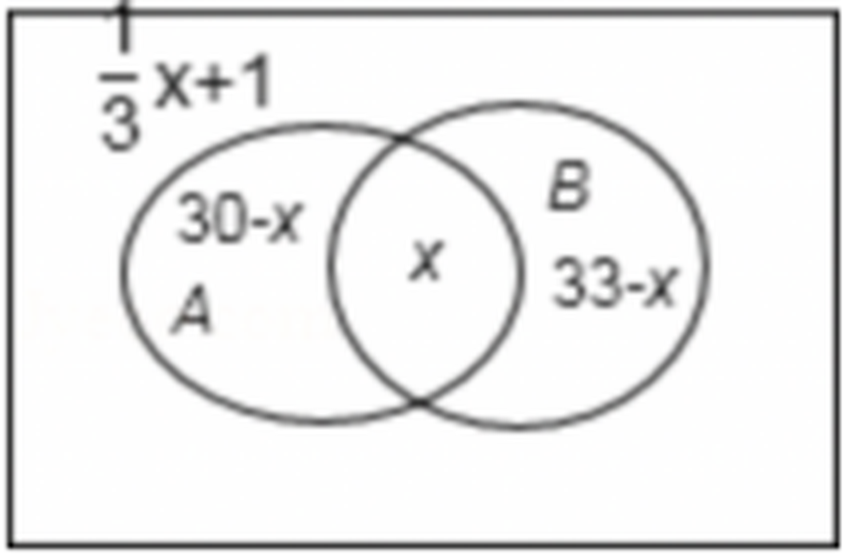
\includegraphics[width=0.30\textwidth]{figures/venn_AB_survey_50.png}
\end{center}

\ans{$21$}

\ifanswer
\solbegin
\step{由题意得赞成 $A$ 的人数 30，赞成 $B$ 的人数为 33，}
\step{设对 $A$、$B$ 都赞成的学生数为 $x$，则对 $A$、$B$ 都不赞成的学生数 $\dfrac{1}{3}x+1$，}
\step{如图得 $x+30-x+33-x+\dfrac{1}{3}x+1=50$，所以 $x=21$.}
\solend

\fi

\item 集合 $S=\{s\mid s=2n+1,n\in\Z\}$，$T=\{t\mid t=4n+1,n\in\Z\}$，则 $S$ \blankline[2.4em] $T$（填“$\subset$”“$\supset$”“$\subseteq$”或“$\supseteq$”）.

\ans{$S\supset T$}

\ifanswer
\solbegin
\step{对于 $S=\{s\mid s=2n+1,n\in\Z\}$ 为奇数，}
\step{而 $T=\{t\mid t=4n+1,n\in\Z\}$ 被 4 整除余 1 的奇数，所以 $S\supset T$.}
\solend

\fi

\item 已知集合 $A=\{x\mid -2<x<4\}$，$B=\{x\mid x^2-3ax+2a^2=0\}$，若 $A\cap B=B$，则实数 $a$ 的取值范围为 \blankline[4.4em].

\ans{$(-1,2)$}

\ifanswer
\solbegin
\step{因为 $A\cap B=B$，所以 $B\subseteq A$，}
\step{①当 $a=0$ 时，方程 $x^2-3ax+2a^2=0$ 的解为 $0$，$B\subseteq A$ 成立；}
\step{②当 $a\neq 0$ 时，方程 $x^2-3ax+2a^2=0$ 的解为 $2a$、$a$，}
\step{则 $-2<2a<4$ 且 $-2<a<4$，解得 $-1<a<2$ 且 $a\neq 0$；}
\step{综上所述，实数 $a$ 的取值范围为 $(-1,2)$.}
\solend

\fi

\item 当一个非空数集 $F$ 满足条件“若 $a$、$b\in F$，则 $a+b$、$a-b$、$ab\in F$，且当 $b\neq 0$ 时，$\dfrac{a}{b}\in F$”时，称 $F$ 为一个数域，以下四个关于数域的命题：

（1）$0$ 是任何数域的元素；（2）若数域 $F$ 有非零元素，则 $2026\in F$；

（3）集合 $P=\{x\mid x=3k,k\in\Z\}$ 为数域；（4）有理数集为数域；

其中，真命题的编号为 \blankline[4.4em]（写出所有真命题的编号）.

\ans{（1）（2）（4）}

\item 对于集合 $M$，定义函数 $f_M(x)=\begin{cases}-1,&x\in M\\ 1,&x\notin M\end{cases}$，对于两个集合 $M$、$N$，定义集合
$M\triangle N=\{x\mid f_M(x)\cdot f_N(x)=-1\}$，已知 $A=\{2,4,6,8,10\},B=\{1,2,4,8,16\}$，用 $|M|$ 表示有限集合 $M$ 中的元素个数，则对于任意集合 $M$，$|M\triangle A|+|M\triangle B|$ 的最小值为 \blankline[2.4em].

% 注：上面分段函数的第二行，原卷印作「1, $x\in M$」（两行都印 $x\in M$），与函数的定义矛盾，
%     本稿按文意订正为 $x\notin M$.
\ans{$4$}

\ifanswer
\solbegin
% 注：下面一行原卷印作「即 $M\triangle N\in\{x\mid x\in M\cup N\}$ 且 $x\in M\cap N$」，「$\in$」当为
%     「$=$」之误，且由 $f_M(x)f_N(x)=-1$ 应对应 $x\notin M\cap N$，本稿一并按文意订正.
\step{由 $M\triangle N$ 的定义得 $f_M(x)\cdot f_N(x)=-1$，}
\step{即 $M\triangle N=\{x\mid x\in M\cup N\text{ 且 }x\notin M\cap N\}$，}
\step{$|M\triangle A|+|M\triangle B|$ 要取得最小值，需满足 $A\cap B\subseteq M\subseteq A\cup B$，}
\step{此时 $|M\triangle A|+|M\triangle B|$ 的最小值为 $4$.}
\solend

\fi

\end{enumerate}

\bigsec{二、选择题}

\begin{enumerate}
\setcounter{enumi}{12}

\item 已知集合 $A=\{x\mid x=3m,m\in\N\}$，$B=\{x\mid x=3m+1,m\in\N\}$，$C=\{x\mid x=3m+2,m\in\N\}$，若 $a\in A$，$b\in B$，$c\in C$，则下列结论中可能成立的是\mbox{（\quad）}

\keepwithprev
A. $2021=a+b+c$\qquad B. $2021=abc$\qquad C. $2021=a+bc$\qquad D. $2021=a(b+c)$

\ans{C}

\ifanswer
\solbegin
\step{由题意设 $a=3m$，$b=3p+1$，$c=3n+2$，$m$、$p$、$n\in\N$，}
\step{则 $a+b+c=3m+3p+1+3n+2=3(m+p+n+1)$，}
\step{故 2021 不是 3 的整数倍，则 A 不可能；}
\step{$abc=3m(3p+1)(3n+2)$，同理 B 不可能；}
\step{$a+bc=3m+(3p+1)(3n+2)=3(m+3pn+2p+n)+2$，$2021=3\times 673+2$，}
\step{如取 $p=n=1$，则 $m=667$，即 $2021=3\times 667+4\times 5$，故 C 成立；}
\step{$a(b+c)=3m(3p+1+3n+2)=9m(p+n+1)$，同 A 可得 D 不可能.}
\step{故选 C.}
\solend

\fi

\item 设 $a$、$b$、$c$ 是实数，$x=a^2-2b+\dfrac{\pi}{3}$，$y=b^2-2c+\dfrac{\pi}{6}$，$z=c^2-2a+\dfrac{\pi}{2}$，则 $x$、$y$、$z$ 中至少有一个值\mbox{（\quad）}

\keepwithprev
A. 大于 $0$\qquad B. 等于 $0$\qquad C. 不大于 $0$\qquad D. 小于 $0$

\ans{A}

\ifanswer
\solbegin
\step{因为 $x+y+z=a^2-2b+\dfrac{\pi}{3}+b^2-2c+\dfrac{\pi}{6}+c^2-2a+\dfrac{\pi}{2}=(a-1)^2+(b-1)^2+(c-1)^2+\pi-3>0$，}
\step{假设 $x$、$y$、$z$ 都不大于 $0$，即 $x\leqslant 0$，$y\leqslant 0$，$z\leqslant 0$，}
\step{由同向不等式的可加性得 $x+y+z\leqslant 0$①，又 $x+y+z>0$ 与①式矛盾.}
\step{所以假设不成立，即原命题的结论 $x$、$y$、$z$ 中至少有一个大于 $0$. 故选 A.}
\solend

\fi

\item 命题“存在一个无理数，它的平方是有理数”的否定是\mbox{（\quad）}

\keepwithprev
A. 任意一个有理数，它的平方是有理数

B. 任意一个无理数，它的平方不是有理数

C. 存在一个有理数，它的平方是有理数

D. 存在一个无理数，它的平方不是有理数

\ans{B}

\ifanswer
\solbegin
\step{否定是任意一个无理数，它的平方不是有理数，故选 B.}
\solend

\fi

\item 设集合 $P_1=\{x\mid x^2+ax+1>0\}$，$P_2=\{x\mid x^2+ax+2>0\}$，$Q_1=\{x\mid x^2+x+b>0\}$，$Q_2=\{x\mid x^2+2x+b>0\}$，其中 $a$、$b\in\R$，下列说法正确的是\mbox{（\quad）}

\keepwithprev
A. 对任意 $a$，$P_1$ 是 $P_2$ 的子集，对任意 $b$，$Q_1$ 不是 $Q_2$ 的子集

B. 对任意 $a$，$P_1$ 是 $P_2$ 的子集，存在 $b$，使得 $Q_1$ 是 $Q_2$ 的子集

C. 对任意 $a$，使得 $P_1$ 不是 $P_2$ 的子集，对任意 $b$，$Q_1$ 不是 $Q_2$ 的子集

D. 对任意 $a$，使得 $P_1$ 不是 $P_2$ 的子集，存在 $b$，使得 $Q_1$ 不是 $Q_2$ 的子集

\ans{B}

\ifanswer
\solbegin
\step{对于集合 $P_1=\{x\mid x^2+ax+1>0\}$，$P_2=\{x\mid x^2+ax+2>0\}$，}
\step{得当 $m\in P_1$，即 $m^2+am+1>0$，得 $m^2+am+2>0$，}
\step{即有 $m\in P_2$，得对任意 $a$，$P_1$ 是 $P_2$ 的子集；}
\step{当 $b=5$ 时，$Q_1=\{x\mid x^2+x+5>0\}=\R$，$Q_2=\{x\mid x^2+2x+5>0\}=\R$，}
\step{得 $Q_1$ 是 $Q_2$ 的子集，故 A 错误，B 正确；}
\step{当 $b=1$ 时，$Q_1=\{x\mid x^2+x+1>0\}=\R$，}
\step{$Q_2=\{x\mid x^2+2x+1>0\}=\{x\mid x\neq -1\text{ 且 }x\in\R\}$，得 $Q_1$ 不是 $Q_2$ 的子集.}
\step{综上，对任意 $a$，$P_1$ 是 $P_2$ 的子集，存在 $b$，使得 $Q_1$ 是 $Q_2$ 的子集，}
\step{故 C 错误，D 错误.}
\step{故选 B.}
\solend

\fi

\end{enumerate}

\bigsec{三、解答题}

\begin{enumerate}
\setcounter{enumi}{16}

\item 已知集合 $A=\{x\mid 0<x-a\leqslant 5\}$，$B=\left\{x\mid -\dfrac{a}{2}<x\leqslant 6\right\}$.

\begin{enumerate}[label=(\arabic*)]
\item 若 $A\subseteq B$，求 $a$ 的取值范围.
\item 集合 $A$ 与 $B$ 能否相等？若能，求出 $a$ 的值，若不能，请说明理由.
\end{enumerate}

\ans{（1）$0\leqslant a\leqslant 1$；（2）不能，$a\in\varnothing$}

\ifanswer
\solbegin
\stepm{（1）}{由于 $A\subseteq B$，所以 $a+5\leqslant 6$，且 $-\dfrac{a}{2}\leqslant a$，解得 $0\leqslant a\leqslant 1$；}
\stepm{（2）}{$A=B$ 时，$a+5=6$，$-\dfrac{a}{2}=a$，解得 $a\in\varnothing$.}
\solend

\fi

\ansspace[6]

\item 已知 $\alpha:2x+m<0$，$\beta:-1<x<3$.

\begin{enumerate}[label=(\arabic*)]
\item 是否存在实数 $m$，使得 $\alpha$ 是 $\beta$ 的充分条件？若存在，求出实数 $m$ 的取值范围；
\item 是否存在实数 $m$，使得 $\alpha$ 是 $\beta$ 的必要条件？若存在，求出实数 $m$ 的取值范围.
\end{enumerate}

\ans{（1）不存在；（2）存在，$m\leqslant -6$}

\ansspace[6]

\item 已知 $\triangle ABC$ 的三边长分别为 $a,b,c$，证明：

\begin{enumerate}[label=(\arabic*)]
\item “$A=90^\circ$”是“关于 $x$ 的方程 $x^2+2ax+b^2=0$ 与 $x^2+2cx-b^2=0$ 有公共实根”的充分条件；
\item “$a=c$”是“关于 $x$ 的方程 $x^2+2ax+b^2=0$ 与 $x^2+2cx-b^2=0$ 没有公共实根”的充分非必要条件.
\end{enumerate}

\ans{（1）略；（2）略}

\ansspace[8]

\item 已知集合 $A$ 包含有 $n(n\in\N^*)$ 个元素，$A^+=\{x+y\mid x\text{、}y\in A\}$.

\begin{enumerate}[label=(\arabic*)]
\item 若 $A=\{0,1,2\}$，写出 $A^+$；
\item % 注：原卷此处印作「写出一个 $A^+$，使得 $A=A^+$」——$A$ 未给定，该问无法作答，
      %     与下方【解析】「取 $A=\{0\}$」不符，本稿按文意订正为「写出一个 $A$」.
      写出一个 $A$，使得 $A=A^+$；
\item 当 $n=4$ 时，是否存在集合 $A$，使得 $A^+=\{2,3,5,6,7,8,10\}$？若存在，求出此时的集合 $A$，若不存在，请说明理由.
\end{enumerate}

\ans{（1）$\{0,1,2,3,4\}$；（2）$A=\{0\}$；（3）不存在}

\ifanswer
\solbegin
\stepm{（1）}{由题意得 $0+0=0$，$0+1=1$，$0+2=2$，$1+1=2$，$1+2=3$，$2+2=4$ 都是 $A^+$ 中的元素，故 $A^+=\{0,1,2,3,4\}$；}
\stepm{（2）}{取 $A=\{0\}$，此时 $A^+=\{x+y\mid x\text{、}y\in A\}=\{0\}$，符合 $A=A^+$；}
\stepm{（3）}{当 $n=4$ 时，不存在集合 $A$，使得 $A^+=\{2,3,5,6,7,8,10\}$，理由如下：}
\step{假设存在 $A=\{a,b,c,d\}$，且 $a<b<c<d$，}
\step{则 $2a<a+b<a+c<b+c<b+d<c+d<2d$，}
\step{故 $2a,a+b,a+c,b+c,b+d,c+d,2d$ 为 $A^+$ 中 7 个不同的元素，}
\step{则 $2a=2$，$a+b=3$，$a+c=5$，$b+c=6$，$b+d=7$，$c+d=8$，$2d=10$，}
\step{解得 $a=1$，$b=2$，$c=4$，$d=5$，}
\step{此时 $c+d=9\in A^+$ 与 $9\notin A^+$ 矛盾，故假设不成立，}
\step{即不存在这样的集合 $A$.}
\solend

\fi

\ansspace[8]

% 压轴题：在其 \item 前先量一下版面，本页剩余高度不足 7cm 就另起一页。
\ansneed{7cm}

\item 已知集合 $A$ 为非空数集，对于集合 $A$，对 $A$ 中任意两个不同元素相加得到的和取绝对值，将这些绝对值重新组成一个新的集合，对于这一过程，我们定义为“自相加”，重新组成的集合叫做“集合 $A$ 的 1 次自相加集合”，再进行 $n-1$ 次“自相加”操作，组成的集合叫做“集合 $A$ 的 $n$ 次自相加集合”. 若集合 $A$ 的任意 $k$ 次自相加集合都不相等，则称集合 $A$ 为“完美自相加集合”，同理，我们可以定义出“$A$ 的 1 次自相减集合”，集合 $A$ 的 1 次自相加集合和 1 次自相减集合分别可表示为：$A^+=\{x\mid x=|a+b|,\ a\text{、}b\in A\}$，$A^-=\{x\mid x=|a-b|,\ a\text{、}b\in A\}$.

\begin{enumerate}[label=(\arabic*)]
\item 已知有两个集合，集合 $B=\{1,2,3,4\}$，集合 $C=\{k\mid k=2n+1,n\in\Z\}$，判断集合 $B$ 和集合 $C$ 是否是完美自相加集合，并说明理由；
\item 对（1）中的集合 $B$ 进行 11 次自相加操作后，求：集合 $B$ 的 11 次自相加集合的元素个数；
\item 若 $0\leqslant n\leqslant 2025$ 且 $n\in\N$，集合 $A=\{x\mid n\leqslant x\leqslant 2025,x\in\N\}$，$A^+\cap A^-=\varnothing$，求：$n$ 的最小值.
\end{enumerate}

\ans{（1）$B$ 是完美自相加集合，$C$ 不是完美自相加集合；（2）$2051$；（3）$675$}

\ifanswer
\solbegin
\stepm{（1）}{$B$ 是完美自相加集合，$C$ 不是完美自相加集合，}
\step{理由如下：因为集合 $B=\{1,2,3,4\}$，所以 $B^+=\{3,4,5,6,7\}$，}
\step{由此可得集合自相加后，}
\step{新的集合中最小的元素为自相加之前的集合中的最小两个元素之和，}
\step{所以显然集合 $B=\{1,2,3,4\}$ 的最小两个元素为 $1$，$2$，}
\step{所以 $B^+$ 中的最小元素为 $1+2=3$，}
\step{同理，2 次自相加后得到的集合中的最小元素是 $3+4=7$.}
\step{依照这样的规律，对集合 $B=\{1,2,3,4\}$ 进行任意次自相加操作后，}
\step{最小值总在变大，故不可能有相等集合，所以 $B$ 是完美自相加集合；}
\step{因为集合 $C=\{k\mid k=2n+1,n\in\Z\}$ 表示所有奇数构成的集合，}
\step{任何两个奇数相加的和都是偶数，}
\step{所以 $C^+=\{k\mid k=2n,n\in\Z\}$ 为所有偶数构成集合；}
\step{所以对 $C^+=\{k\mid k=2n,n\in\Z\}$ 再进行一次自相加操作，}
\step{因为任意两个偶数相加的和还是偶数，}
\step{所以后面集合不管进行多少次相加都与 $C^+=\{k\mid k=2n,n\in\Z\}$ 相同；}
\step{故 $C$ 不是完美自相加集合.}
\stepm{（2）}{由自相加性质得，对于集合 $B=\{1,2,3,4\}$，进行一次自相加，}
\step{得到集合的最小值必然是原来集合的两个最小元素值之和，}
\step{得到的最大值必然为原来集合的两个最大元素值之和，}
\step{且中间必然是连续的整数元素；}
\step{所以对集合 $B=\{1,2,3,4\}$ 进行 1 次自相加之后，}
\step{得到的集合最小两个元素为 $3$，$4$，最大的两个元素为 $6$，$7$；}
\step{进行第 2 次自相加，得到的集合最小两个元素为 $7$，$8$，}
\step{最大的两个元素为 $12$，$13$；}
\step{进行第 3 次自相加，得到的集合最小两个元素为 $15$，$16$，}
\step{最大的两个元素为 $24$，$25$；}
\step{进行第 4 次自相加，得到的集合最小两个元素为 $31$，$32$，}
\step{最大的两个元素为 $48$，$49$；}
\step{进行第 5 次自相加，得到的集合最小两个元素为 $63$，$64$，}
\step{最大的两个元素为 $96$，$97$；}
\step{进行第 6 次自相加，得到的集合最小两个元素为 $127$，$128$，}
\step{最大的两个元素为 $192$，$193$；}
\step{进行第 7 次自相加，得到的集合最小两个元素为 $255$，$256$，}
\step{最大的两个元素为 $384$，$385$；}
\step{进行第 8 次自相加，得到的集合最小两个元素为 $511$，$512$，}
\step{最大的两个元素为 $768$，$769$；}
\step{进行第 9 次自相加，得到的集合最小两个元素为 $1023$，$1024$，}
\step{最大的两个元素为 $1536$，$1537$；}
\step{进行第 10 次自相加，得到的集合最小两个元素为 $2047$，$2048$，}
\step{最大的两个元素为 $3072$，$3073$；}
\step{进行第 11 次自相加，得到的集合最小两个元素为 $4095$，$4096$，}
\step{最大的两个元素为 $6144$，$6145$；}
\step{因为集合 $B$ 的 $n$ 次自相加集合中的元素都是连续的整数，}
\step{所以集合 $B$ 进行 11 次自相加操作后的元素个数为 $6145-4095+1=2051$.}
\stepm{（3）}{因为 $0\leqslant n\leqslant 2025$ 且 $n\in\N$，集合 $A=\{x\mid n\leqslant x\leqslant 2025,x\in\N\}$，}
\step{所以 $A^+=\{x\mid 2n+1\leqslant x\leqslant 4049,x\in\N\}$，}
\step{$A^-=\{x\mid 1\leqslant x\leqslant 2025-n,x\in\N\}$，}
\step{要使 $A^+\cap A^-=\varnothing$，须使 $2n+1>2025-n$，所以 $n>\dfrac{2024}{3}=674\dfrac{2}{3}$，}
\step{又 $n\in\N$，故 $n$ 的最小值为 $675$.}
\solend

\fi

% 压轴题：其后已无内容，故作答区全用可丢弃胶水（\ansspace*）。
\ansspace*[12]

\end{enumerate}

\end{document}
"
% 紧凑版：xelatex "\def\iscompact{1}% 高一17_七宝中学_周末作业2.tex —— 高一上数学「2026-2027 年七宝中学高一上周末作业 2」（试卷版/答案版）
% 试卷版：xelatex 高一17_七宝中学_周末作业2.tex
% 答案版：xelatex "\def\isanswer{1}% 高一17_七宝中学_周末作业2.tex —— 高一上数学「2026-2027 年七宝中学高一上周末作业 2」（试卷版/答案版）
% 试卷版：xelatex 高一17_七宝中学_周末作业2.tex
% 答案版：xelatex "\def\isanswer{1}% 高一17_七宝中学_周末作业2.tex —— 高一上数学「2026-2027 年七宝中学高一上周末作业 2」（试卷版/答案版）
% 试卷版：xelatex 高一17_七宝中学_周末作业2.tex
% 答案版：xelatex "\def\isanswer{1}\input{高一17_七宝中学_周末作业2.tex}"
% 紧凑版：xelatex "\def\iscompact{1}\input{高一17_七宝中学_周末作业2.tex}"
%
% 原始材料是微信公众号图文（公众号「魔都数学加油站」），正文为 10 张 PNG 页（1080×1527）。
% 原文本身就是一份**讲评版**——题目下方直接印出【答案】或【解析】，选择题的答案印在解析末句
% 「故选 X」里。试题文字、答案与解析均照原卷录入（订正处见下），卷面上的粉色斜水印
% 「魔都数学加油站」属水印，未录入。
%
% 与原卷的排版差异（均已在 README「说明」中交代）：
%   ① 原文自**第 3 题**起（第 1、2 题未在该文中发布），故本稿题号亦自 3 起；
%   ② 原卷本就印有「一、填空题」「二、选择题」「三、解答题」三节标题（分别在原图 00/02/04.png
%      上，逐页核对过），本稿照原卷分节，只把标题改排成全稿统一的「大节标题」样式；
%   ③ 原卷填空、选择的答案直接印在题目下方（选择题只在解析末句「故选 X」中给出），本稿统一改为
%      试卷版隐去、答案版以【答案】给出，选择题的括注一律改排「\mbox{（\quad）}」并把答案移到选项之后，
%      使两版彻底分离；
%   ④ 原卷的集合符号大小写混用：第 3 题题干的实数集印成**粗体** $\mathbf{R}$，第 16 题题干与
%      第 16 题解析的印成正体 $R$；自然数集 $N$、整数集 $Z$ 一律正体。本稿按全稿惯例统一写作
%      $\R$、$\N$、$\Z$；
%   ⑤ 原卷未印副标题，本稿按全稿惯例补出副标题「集合与常用逻辑用语」；
%   ⑥ 原卷解答题子问编号为「（1）（2）」，本稿用嵌套 enumerate 排成同一形态；原卷第 15 题的
%      D 选项因原页翻页被截到下一页首页，本稿自然连排；
%   ⑦ 原卷解答题未留作答空间（讲评稿通篇是答案），本稿逐题补出书写留白，仅试卷版显示；
%   ⑧ 第 21 题题干里 $A^+$、$A^-$ 的定义含绝对值号（原卷作 $\{x\mid x=|a+b|,\ a\text{、}b\in A\}$
%      与 $\{x\mid x=|a-b|,\ a\text{、}b\in A\}$），本稿照原卷录入；2026-09-15 回原图逐处放大复核
%      时发现曾漏抄两处绝对值号、并把分隔逗号误写成 $\mid$，已按原卷订正（见 README 专记）。
%
% 原卷笔误三处（均已放大到能看清字形后核对，本稿按文意订正，并在 README 中写明原委）：
%   ① 第 12 题题干的分段函数 $f_M(x)$ 原卷两行都印作「$x\in M$」（$-1$ 与 $1$ 都取在 $M$ 上），
%      与「函数」的定义直接矛盾（$M$ 上无法同时取两个值），按文意订正第二行为 $x\notin M$；
%   ② 第 12 题【解析】首行原卷印「即 $M\triangle N\in\{x\mid x\in M\cup N\}$ 且 $x\in M\cap N$」，
%      其中「$\in$」当为「$=$」之误；且由 $f_M(x)f_N(x)=-1$ 应对应 $x\notin M\cap N$（原卷印作
%      $x\in M\cap N$，与上一行刚写出的对称差的定义相矛盾），本稿一并订正；
%   ③ 第 20 题(2)原卷印「写出一个 $A^+$，使得 $A=A^+$」——$A$ 未给定，该问无法作答，与紧接的
%      【解析】「取 $A=\{0\}$，此时 $A^+=\{0\}$，符合 $A=A^+$」不符，本稿按文意订正为
%      「写出一个 $A$，使得 $A=A^+$」.
%
% 原卷存疑一处（无法确证原意，本稿照抄原卷、未改）：
%   ① 第 5 题 ④ 原卷题干印 $S=\{x\mid |x|\leqslant\sqrt{3},x\in N\}$（该字母与 ③ 中的 $Z$
%      字形明显不同，$Z$ 有上下两横，已放大比对确认），而【解析】印「因为 $S=\{-1,0,1\}$」——
%      按 $x\in N$ 应为 $S=\{0,1\}$（或 $\{1\}$），题干与解析的口径不一致；但无论取哪一口径，
%      ④ 都是 $M$ 的子集、本题结论（填④）不变，故题干与解析均照抄原卷，未改。

\documentclass[a4paper,11pt]{article}
\usepackage{common}

\begin{document}

\examtitlest{2026--2027 年七宝中学高一上周末作业 2}{集合与常用逻辑用语}

\bigsec{一、填空题}

\begin{enumerate}
\setcounter{enumi}{2}

\item 已知 $a,x\in\R$，则“$x\in\{-a,a\}$”是“$|x|=a$”的 \blankline[4.4em] 条件.

\ans{必要不充分}

\item 设全集为 $U$，$A\subseteq U$，$B\subseteq U$，则“$A\subset B$”是“$\overline{B}\subset\overline{A}$”的 \blankline[4.4em] 条件.

\ans{充要}

\item 已知集合 $M=\{x\mid -\sqrt{5}<x<\sqrt{3},x\in\Z\}$，则下列集合是集合 $M$ 的子集的是 \blankline[4.4em]（填序号）.

① $P=\{-3,0,1\}$；② $Q=\{-1,0,1,2\}$；③ $R=\{y\mid -\pi<y<-1,y\in\Z\}$；

④ $S=\{x\mid |x|\leqslant\sqrt{3},x\in\N\}$.

\ans{④}

\ifanswer
\solbegin
\step{由已知得集合 $M=\{-2,-1,0,1\}$，}
\step{所以由子集的定义得选项①错误，②错误，}
\step{因为 $R=\{-3,-2\}$，所以集合 $R$ 不表示集合 $M$ 的子集，③错误，}
\step{因为 $S=\{-1,0,1\}$，所以是集合 $M$ 的子集，故正确.}
\step{故是集合 $M$ 的子集的是④.}
\solend

\fi

\item 已知 $x\in\R$，用反证法证明命题“若 $x^2-7x+10<0$，则 $2<x<5$”时，应该假设 \blankline[5em].

\ans{$x\leqslant 2$ 或 $x\geqslant 5$}

\item 设 $a_1,b_1,c_1,a_2,b_2,c_2$ 均为非零实数，方程 $a_1x^2+b_1x+c_1=0$ 和 $a_2x^2+b_2x+c_2=0$ 的解集分别为 $M$ 和 $N$，那么“$\dfrac{a_1}{a_2}=\dfrac{b_1}{b_2}=\dfrac{c_1}{c_2}$”是“$M=N$”的 \blankline[4.4em] 条件.

（填“充分非必要”、“必要非充分”、“充要”、或“既非充分又非必要”）

\ans{充分非必要}

\ifanswer
\solbegin
\step{$\dfrac{a_1}{a_2}=\dfrac{b_1}{b_2}=\dfrac{c_1}{c_2}$ 能推出 $M=N$，}
\step{若 $M=N=\varnothing$ 推不出 $\dfrac{a_1}{a_2}=\dfrac{b_1}{b_2}=\dfrac{c_1}{c_2}$，}
\step{所以“$\dfrac{a_1}{a_2}=\dfrac{b_1}{b_2}=\dfrac{c_1}{c_2}$”是“$M=N$”的“充分非必要”条件.}
\solend

\fi

\item 向 50 名学生调查对 $A$、$B$ 两事件的态度，有如下结果赞成 $A$ 的人数是全体的五分之三，其余的不赞成，赞成 $B$ 的比赞成 $A$ 的多 3 人，其余的不赞成；另外，对 $A$、$B$ 都不赞成的学生数比对 $A$、$B$ 都赞成的学生数的三分之一多 1 人. 则对 $A$、$B$ 都赞成的学生有 \blankline[2.4em] 人.

\begin{center}
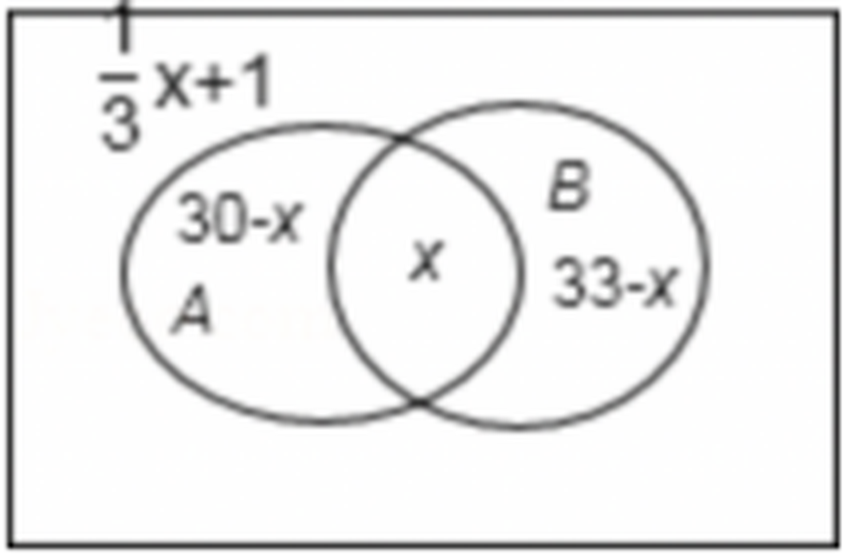
\includegraphics[width=0.30\textwidth]{figures/venn_AB_survey_50.png}
\end{center}

\ans{$21$}

\ifanswer
\solbegin
\step{由题意得赞成 $A$ 的人数 30，赞成 $B$ 的人数为 33，}
\step{设对 $A$、$B$ 都赞成的学生数为 $x$，则对 $A$、$B$ 都不赞成的学生数 $\dfrac{1}{3}x+1$，}
\step{如图得 $x+30-x+33-x+\dfrac{1}{3}x+1=50$，所以 $x=21$.}
\solend

\fi

\item 集合 $S=\{s\mid s=2n+1,n\in\Z\}$，$T=\{t\mid t=4n+1,n\in\Z\}$，则 $S$ \blankline[2.4em] $T$（填“$\subset$”“$\supset$”“$\subseteq$”或“$\supseteq$”）.

\ans{$S\supset T$}

\ifanswer
\solbegin
\step{对于 $S=\{s\mid s=2n+1,n\in\Z\}$ 为奇数，}
\step{而 $T=\{t\mid t=4n+1,n\in\Z\}$ 被 4 整除余 1 的奇数，所以 $S\supset T$.}
\solend

\fi

\item 已知集合 $A=\{x\mid -2<x<4\}$，$B=\{x\mid x^2-3ax+2a^2=0\}$，若 $A\cap B=B$，则实数 $a$ 的取值范围为 \blankline[4.4em].

\ans{$(-1,2)$}

\ifanswer
\solbegin
\step{因为 $A\cap B=B$，所以 $B\subseteq A$，}
\step{①当 $a=0$ 时，方程 $x^2-3ax+2a^2=0$ 的解为 $0$，$B\subseteq A$ 成立；}
\step{②当 $a\neq 0$ 时，方程 $x^2-3ax+2a^2=0$ 的解为 $2a$、$a$，}
\step{则 $-2<2a<4$ 且 $-2<a<4$，解得 $-1<a<2$ 且 $a\neq 0$；}
\step{综上所述，实数 $a$ 的取值范围为 $(-1,2)$.}
\solend

\fi

\item 当一个非空数集 $F$ 满足条件“若 $a$、$b\in F$，则 $a+b$、$a-b$、$ab\in F$，且当 $b\neq 0$ 时，$\dfrac{a}{b}\in F$”时，称 $F$ 为一个数域，以下四个关于数域的命题：

（1）$0$ 是任何数域的元素；（2）若数域 $F$ 有非零元素，则 $2026\in F$；

（3）集合 $P=\{x\mid x=3k,k\in\Z\}$ 为数域；（4）有理数集为数域；

其中，真命题的编号为 \blankline[4.4em]（写出所有真命题的编号）.

\ans{（1）（2）（4）}

\item 对于集合 $M$，定义函数 $f_M(x)=\begin{cases}-1,&x\in M\\ 1,&x\notin M\end{cases}$，对于两个集合 $M$、$N$，定义集合
$M\triangle N=\{x\mid f_M(x)\cdot f_N(x)=-1\}$，已知 $A=\{2,4,6,8,10\},B=\{1,2,4,8,16\}$，用 $|M|$ 表示有限集合 $M$ 中的元素个数，则对于任意集合 $M$，$|M\triangle A|+|M\triangle B|$ 的最小值为 \blankline[2.4em].

% 注：上面分段函数的第二行，原卷印作「1, $x\in M$」（两行都印 $x\in M$），与函数的定义矛盾，
%     本稿按文意订正为 $x\notin M$.
\ans{$4$}

\ifanswer
\solbegin
% 注：下面一行原卷印作「即 $M\triangle N\in\{x\mid x\in M\cup N\}$ 且 $x\in M\cap N$」，「$\in$」当为
%     「$=$」之误，且由 $f_M(x)f_N(x)=-1$ 应对应 $x\notin M\cap N$，本稿一并按文意订正.
\step{由 $M\triangle N$ 的定义得 $f_M(x)\cdot f_N(x)=-1$，}
\step{即 $M\triangle N=\{x\mid x\in M\cup N\text{ 且 }x\notin M\cap N\}$，}
\step{$|M\triangle A|+|M\triangle B|$ 要取得最小值，需满足 $A\cap B\subseteq M\subseteq A\cup B$，}
\step{此时 $|M\triangle A|+|M\triangle B|$ 的最小值为 $4$.}
\solend

\fi

\end{enumerate}

\bigsec{二、选择题}

\begin{enumerate}
\setcounter{enumi}{12}

\item 已知集合 $A=\{x\mid x=3m,m\in\N\}$，$B=\{x\mid x=3m+1,m\in\N\}$，$C=\{x\mid x=3m+2,m\in\N\}$，若 $a\in A$，$b\in B$，$c\in C$，则下列结论中可能成立的是\mbox{（\quad）}

\keepwithprev
A. $2021=a+b+c$\qquad B. $2021=abc$\qquad C. $2021=a+bc$\qquad D. $2021=a(b+c)$

\ans{C}

\ifanswer
\solbegin
\step{由题意设 $a=3m$，$b=3p+1$，$c=3n+2$，$m$、$p$、$n\in\N$，}
\step{则 $a+b+c=3m+3p+1+3n+2=3(m+p+n+1)$，}
\step{故 2021 不是 3 的整数倍，则 A 不可能；}
\step{$abc=3m(3p+1)(3n+2)$，同理 B 不可能；}
\step{$a+bc=3m+(3p+1)(3n+2)=3(m+3pn+2p+n)+2$，$2021=3\times 673+2$，}
\step{如取 $p=n=1$，则 $m=667$，即 $2021=3\times 667+4\times 5$，故 C 成立；}
\step{$a(b+c)=3m(3p+1+3n+2)=9m(p+n+1)$，同 A 可得 D 不可能.}
\step{故选 C.}
\solend

\fi

\item 设 $a$、$b$、$c$ 是实数，$x=a^2-2b+\dfrac{\pi}{3}$，$y=b^2-2c+\dfrac{\pi}{6}$，$z=c^2-2a+\dfrac{\pi}{2}$，则 $x$、$y$、$z$ 中至少有一个值\mbox{（\quad）}

\keepwithprev
A. 大于 $0$\qquad B. 等于 $0$\qquad C. 不大于 $0$\qquad D. 小于 $0$

\ans{A}

\ifanswer
\solbegin
\step{因为 $x+y+z=a^2-2b+\dfrac{\pi}{3}+b^2-2c+\dfrac{\pi}{6}+c^2-2a+\dfrac{\pi}{2}=(a-1)^2+(b-1)^2+(c-1)^2+\pi-3>0$，}
\step{假设 $x$、$y$、$z$ 都不大于 $0$，即 $x\leqslant 0$，$y\leqslant 0$，$z\leqslant 0$，}
\step{由同向不等式的可加性得 $x+y+z\leqslant 0$①，又 $x+y+z>0$ 与①式矛盾.}
\step{所以假设不成立，即原命题的结论 $x$、$y$、$z$ 中至少有一个大于 $0$. 故选 A.}
\solend

\fi

\item 命题“存在一个无理数，它的平方是有理数”的否定是\mbox{（\quad）}

\keepwithprev
A. 任意一个有理数，它的平方是有理数

B. 任意一个无理数，它的平方不是有理数

C. 存在一个有理数，它的平方是有理数

D. 存在一个无理数，它的平方不是有理数

\ans{B}

\ifanswer
\solbegin
\step{否定是任意一个无理数，它的平方不是有理数，故选 B.}
\solend

\fi

\item 设集合 $P_1=\{x\mid x^2+ax+1>0\}$，$P_2=\{x\mid x^2+ax+2>0\}$，$Q_1=\{x\mid x^2+x+b>0\}$，$Q_2=\{x\mid x^2+2x+b>0\}$，其中 $a$、$b\in\R$，下列说法正确的是\mbox{（\quad）}

\keepwithprev
A. 对任意 $a$，$P_1$ 是 $P_2$ 的子集，对任意 $b$，$Q_1$ 不是 $Q_2$ 的子集

B. 对任意 $a$，$P_1$ 是 $P_2$ 的子集，存在 $b$，使得 $Q_1$ 是 $Q_2$ 的子集

C. 对任意 $a$，使得 $P_1$ 不是 $P_2$ 的子集，对任意 $b$，$Q_1$ 不是 $Q_2$ 的子集

D. 对任意 $a$，使得 $P_1$ 不是 $P_2$ 的子集，存在 $b$，使得 $Q_1$ 不是 $Q_2$ 的子集

\ans{B}

\ifanswer
\solbegin
\step{对于集合 $P_1=\{x\mid x^2+ax+1>0\}$，$P_2=\{x\mid x^2+ax+2>0\}$，}
\step{得当 $m\in P_1$，即 $m^2+am+1>0$，得 $m^2+am+2>0$，}
\step{即有 $m\in P_2$，得对任意 $a$，$P_1$ 是 $P_2$ 的子集；}
\step{当 $b=5$ 时，$Q_1=\{x\mid x^2+x+5>0\}=\R$，$Q_2=\{x\mid x^2+2x+5>0\}=\R$，}
\step{得 $Q_1$ 是 $Q_2$ 的子集，故 A 错误，B 正确；}
\step{当 $b=1$ 时，$Q_1=\{x\mid x^2+x+1>0\}=\R$，}
\step{$Q_2=\{x\mid x^2+2x+1>0\}=\{x\mid x\neq -1\text{ 且 }x\in\R\}$，得 $Q_1$ 不是 $Q_2$ 的子集.}
\step{综上，对任意 $a$，$P_1$ 是 $P_2$ 的子集，存在 $b$，使得 $Q_1$ 是 $Q_2$ 的子集，}
\step{故 C 错误，D 错误.}
\step{故选 B.}
\solend

\fi

\end{enumerate}

\bigsec{三、解答题}

\begin{enumerate}
\setcounter{enumi}{16}

\item 已知集合 $A=\{x\mid 0<x-a\leqslant 5\}$，$B=\left\{x\mid -\dfrac{a}{2}<x\leqslant 6\right\}$.

\begin{enumerate}[label=(\arabic*)]
\item 若 $A\subseteq B$，求 $a$ 的取值范围.
\item 集合 $A$ 与 $B$ 能否相等？若能，求出 $a$ 的值，若不能，请说明理由.
\end{enumerate}

\ans{（1）$0\leqslant a\leqslant 1$；（2）不能，$a\in\varnothing$}

\ifanswer
\solbegin
\stepm{（1）}{由于 $A\subseteq B$，所以 $a+5\leqslant 6$，且 $-\dfrac{a}{2}\leqslant a$，解得 $0\leqslant a\leqslant 1$；}
\stepm{（2）}{$A=B$ 时，$a+5=6$，$-\dfrac{a}{2}=a$，解得 $a\in\varnothing$.}
\solend

\fi

\ansspace[6]

\item 已知 $\alpha:2x+m<0$，$\beta:-1<x<3$.

\begin{enumerate}[label=(\arabic*)]
\item 是否存在实数 $m$，使得 $\alpha$ 是 $\beta$ 的充分条件？若存在，求出实数 $m$ 的取值范围；
\item 是否存在实数 $m$，使得 $\alpha$ 是 $\beta$ 的必要条件？若存在，求出实数 $m$ 的取值范围.
\end{enumerate}

\ans{（1）不存在；（2）存在，$m\leqslant -6$}

\ansspace[6]

\item 已知 $\triangle ABC$ 的三边长分别为 $a,b,c$，证明：

\begin{enumerate}[label=(\arabic*)]
\item “$A=90^\circ$”是“关于 $x$ 的方程 $x^2+2ax+b^2=0$ 与 $x^2+2cx-b^2=0$ 有公共实根”的充分条件；
\item “$a=c$”是“关于 $x$ 的方程 $x^2+2ax+b^2=0$ 与 $x^2+2cx-b^2=0$ 没有公共实根”的充分非必要条件.
\end{enumerate}

\ans{（1）略；（2）略}

\ansspace[8]

\item 已知集合 $A$ 包含有 $n(n\in\N^*)$ 个元素，$A^+=\{x+y\mid x\text{、}y\in A\}$.

\begin{enumerate}[label=(\arabic*)]
\item 若 $A=\{0,1,2\}$，写出 $A^+$；
\item % 注：原卷此处印作「写出一个 $A^+$，使得 $A=A^+$」——$A$ 未给定，该问无法作答，
      %     与下方【解析】「取 $A=\{0\}$」不符，本稿按文意订正为「写出一个 $A$」.
      写出一个 $A$，使得 $A=A^+$；
\item 当 $n=4$ 时，是否存在集合 $A$，使得 $A^+=\{2,3,5,6,7,8,10\}$？若存在，求出此时的集合 $A$，若不存在，请说明理由.
\end{enumerate}

\ans{（1）$\{0,1,2,3,4\}$；（2）$A=\{0\}$；（3）不存在}

\ifanswer
\solbegin
\stepm{（1）}{由题意得 $0+0=0$，$0+1=1$，$0+2=2$，$1+1=2$，$1+2=3$，$2+2=4$ 都是 $A^+$ 中的元素，故 $A^+=\{0,1,2,3,4\}$；}
\stepm{（2）}{取 $A=\{0\}$，此时 $A^+=\{x+y\mid x\text{、}y\in A\}=\{0\}$，符合 $A=A^+$；}
\stepm{（3）}{当 $n=4$ 时，不存在集合 $A$，使得 $A^+=\{2,3,5,6,7,8,10\}$，理由如下：}
\step{假设存在 $A=\{a,b,c,d\}$，且 $a<b<c<d$，}
\step{则 $2a<a+b<a+c<b+c<b+d<c+d<2d$，}
\step{故 $2a,a+b,a+c,b+c,b+d,c+d,2d$ 为 $A^+$ 中 7 个不同的元素，}
\step{则 $2a=2$，$a+b=3$，$a+c=5$，$b+c=6$，$b+d=7$，$c+d=8$，$2d=10$，}
\step{解得 $a=1$，$b=2$，$c=4$，$d=5$，}
\step{此时 $c+d=9\in A^+$ 与 $9\notin A^+$ 矛盾，故假设不成立，}
\step{即不存在这样的集合 $A$.}
\solend

\fi

\ansspace[8]

% 压轴题：在其 \item 前先量一下版面，本页剩余高度不足 7cm 就另起一页。
\ansneed{7cm}

\item 已知集合 $A$ 为非空数集，对于集合 $A$，对 $A$ 中任意两个不同元素相加得到的和取绝对值，将这些绝对值重新组成一个新的集合，对于这一过程，我们定义为“自相加”，重新组成的集合叫做“集合 $A$ 的 1 次自相加集合”，再进行 $n-1$ 次“自相加”操作，组成的集合叫做“集合 $A$ 的 $n$ 次自相加集合”. 若集合 $A$ 的任意 $k$ 次自相加集合都不相等，则称集合 $A$ 为“完美自相加集合”，同理，我们可以定义出“$A$ 的 1 次自相减集合”，集合 $A$ 的 1 次自相加集合和 1 次自相减集合分别可表示为：$A^+=\{x\mid x=|a+b|,\ a\text{、}b\in A\}$，$A^-=\{x\mid x=|a-b|,\ a\text{、}b\in A\}$.

\begin{enumerate}[label=(\arabic*)]
\item 已知有两个集合，集合 $B=\{1,2,3,4\}$，集合 $C=\{k\mid k=2n+1,n\in\Z\}$，判断集合 $B$ 和集合 $C$ 是否是完美自相加集合，并说明理由；
\item 对（1）中的集合 $B$ 进行 11 次自相加操作后，求：集合 $B$ 的 11 次自相加集合的元素个数；
\item 若 $0\leqslant n\leqslant 2025$ 且 $n\in\N$，集合 $A=\{x\mid n\leqslant x\leqslant 2025,x\in\N\}$，$A^+\cap A^-=\varnothing$，求：$n$ 的最小值.
\end{enumerate}

\ans{（1）$B$ 是完美自相加集合，$C$ 不是完美自相加集合；（2）$2051$；（3）$675$}

\ifanswer
\solbegin
\stepm{（1）}{$B$ 是完美自相加集合，$C$ 不是完美自相加集合，}
\step{理由如下：因为集合 $B=\{1,2,3,4\}$，所以 $B^+=\{3,4,5,6,7\}$，}
\step{由此可得集合自相加后，}
\step{新的集合中最小的元素为自相加之前的集合中的最小两个元素之和，}
\step{所以显然集合 $B=\{1,2,3,4\}$ 的最小两个元素为 $1$，$2$，}
\step{所以 $B^+$ 中的最小元素为 $1+2=3$，}
\step{同理，2 次自相加后得到的集合中的最小元素是 $3+4=7$.}
\step{依照这样的规律，对集合 $B=\{1,2,3,4\}$ 进行任意次自相加操作后，}
\step{最小值总在变大，故不可能有相等集合，所以 $B$ 是完美自相加集合；}
\step{因为集合 $C=\{k\mid k=2n+1,n\in\Z\}$ 表示所有奇数构成的集合，}
\step{任何两个奇数相加的和都是偶数，}
\step{所以 $C^+=\{k\mid k=2n,n\in\Z\}$ 为所有偶数构成集合；}
\step{所以对 $C^+=\{k\mid k=2n,n\in\Z\}$ 再进行一次自相加操作，}
\step{因为任意两个偶数相加的和还是偶数，}
\step{所以后面集合不管进行多少次相加都与 $C^+=\{k\mid k=2n,n\in\Z\}$ 相同；}
\step{故 $C$ 不是完美自相加集合.}
\stepm{（2）}{由自相加性质得，对于集合 $B=\{1,2,3,4\}$，进行一次自相加，}
\step{得到集合的最小值必然是原来集合的两个最小元素值之和，}
\step{得到的最大值必然为原来集合的两个最大元素值之和，}
\step{且中间必然是连续的整数元素；}
\step{所以对集合 $B=\{1,2,3,4\}$ 进行 1 次自相加之后，}
\step{得到的集合最小两个元素为 $3$，$4$，最大的两个元素为 $6$，$7$；}
\step{进行第 2 次自相加，得到的集合最小两个元素为 $7$，$8$，}
\step{最大的两个元素为 $12$，$13$；}
\step{进行第 3 次自相加，得到的集合最小两个元素为 $15$，$16$，}
\step{最大的两个元素为 $24$，$25$；}
\step{进行第 4 次自相加，得到的集合最小两个元素为 $31$，$32$，}
\step{最大的两个元素为 $48$，$49$；}
\step{进行第 5 次自相加，得到的集合最小两个元素为 $63$，$64$，}
\step{最大的两个元素为 $96$，$97$；}
\step{进行第 6 次自相加，得到的集合最小两个元素为 $127$，$128$，}
\step{最大的两个元素为 $192$，$193$；}
\step{进行第 7 次自相加，得到的集合最小两个元素为 $255$，$256$，}
\step{最大的两个元素为 $384$，$385$；}
\step{进行第 8 次自相加，得到的集合最小两个元素为 $511$，$512$，}
\step{最大的两个元素为 $768$，$769$；}
\step{进行第 9 次自相加，得到的集合最小两个元素为 $1023$，$1024$，}
\step{最大的两个元素为 $1536$，$1537$；}
\step{进行第 10 次自相加，得到的集合最小两个元素为 $2047$，$2048$，}
\step{最大的两个元素为 $3072$，$3073$；}
\step{进行第 11 次自相加，得到的集合最小两个元素为 $4095$，$4096$，}
\step{最大的两个元素为 $6144$，$6145$；}
\step{因为集合 $B$ 的 $n$ 次自相加集合中的元素都是连续的整数，}
\step{所以集合 $B$ 进行 11 次自相加操作后的元素个数为 $6145-4095+1=2051$.}
\stepm{（3）}{因为 $0\leqslant n\leqslant 2025$ 且 $n\in\N$，集合 $A=\{x\mid n\leqslant x\leqslant 2025,x\in\N\}$，}
\step{所以 $A^+=\{x\mid 2n+1\leqslant x\leqslant 4049,x\in\N\}$，}
\step{$A^-=\{x\mid 1\leqslant x\leqslant 2025-n,x\in\N\}$，}
\step{要使 $A^+\cap A^-=\varnothing$，须使 $2n+1>2025-n$，所以 $n>\dfrac{2024}{3}=674\dfrac{2}{3}$，}
\step{又 $n\in\N$，故 $n$ 的最小值为 $675$.}
\solend

\fi

% 压轴题：其后已无内容，故作答区全用可丢弃胶水（\ansspace*）。
\ansspace*[12]

\end{enumerate}

\end{document}
"
% 紧凑版：xelatex "\def\iscompact{1}% 高一17_七宝中学_周末作业2.tex —— 高一上数学「2026-2027 年七宝中学高一上周末作业 2」（试卷版/答案版）
% 试卷版：xelatex 高一17_七宝中学_周末作业2.tex
% 答案版：xelatex "\def\isanswer{1}\input{高一17_七宝中学_周末作业2.tex}"
% 紧凑版：xelatex "\def\iscompact{1}\input{高一17_七宝中学_周末作业2.tex}"
%
% 原始材料是微信公众号图文（公众号「魔都数学加油站」），正文为 10 张 PNG 页（1080×1527）。
% 原文本身就是一份**讲评版**——题目下方直接印出【答案】或【解析】，选择题的答案印在解析末句
% 「故选 X」里。试题文字、答案与解析均照原卷录入（订正处见下），卷面上的粉色斜水印
% 「魔都数学加油站」属水印，未录入。
%
% 与原卷的排版差异（均已在 README「说明」中交代）：
%   ① 原文自**第 3 题**起（第 1、2 题未在该文中发布），故本稿题号亦自 3 起；
%   ② 原卷本就印有「一、填空题」「二、选择题」「三、解答题」三节标题（分别在原图 00/02/04.png
%      上，逐页核对过），本稿照原卷分节，只把标题改排成全稿统一的「大节标题」样式；
%   ③ 原卷填空、选择的答案直接印在题目下方（选择题只在解析末句「故选 X」中给出），本稿统一改为
%      试卷版隐去、答案版以【答案】给出，选择题的括注一律改排「\mbox{（\quad）}」并把答案移到选项之后，
%      使两版彻底分离；
%   ④ 原卷的集合符号大小写混用：第 3 题题干的实数集印成**粗体** $\mathbf{R}$，第 16 题题干与
%      第 16 题解析的印成正体 $R$；自然数集 $N$、整数集 $Z$ 一律正体。本稿按全稿惯例统一写作
%      $\R$、$\N$、$\Z$；
%   ⑤ 原卷未印副标题，本稿按全稿惯例补出副标题「集合与常用逻辑用语」；
%   ⑥ 原卷解答题子问编号为「（1）（2）」，本稿用嵌套 enumerate 排成同一形态；原卷第 15 题的
%      D 选项因原页翻页被截到下一页首页，本稿自然连排；
%   ⑦ 原卷解答题未留作答空间（讲评稿通篇是答案），本稿逐题补出书写留白，仅试卷版显示；
%   ⑧ 第 21 题题干里 $A^+$、$A^-$ 的定义含绝对值号（原卷作 $\{x\mid x=|a+b|,\ a\text{、}b\in A\}$
%      与 $\{x\mid x=|a-b|,\ a\text{、}b\in A\}$），本稿照原卷录入；2026-09-15 回原图逐处放大复核
%      时发现曾漏抄两处绝对值号、并把分隔逗号误写成 $\mid$，已按原卷订正（见 README 专记）。
%
% 原卷笔误三处（均已放大到能看清字形后核对，本稿按文意订正，并在 README 中写明原委）：
%   ① 第 12 题题干的分段函数 $f_M(x)$ 原卷两行都印作「$x\in M$」（$-1$ 与 $1$ 都取在 $M$ 上），
%      与「函数」的定义直接矛盾（$M$ 上无法同时取两个值），按文意订正第二行为 $x\notin M$；
%   ② 第 12 题【解析】首行原卷印「即 $M\triangle N\in\{x\mid x\in M\cup N\}$ 且 $x\in M\cap N$」，
%      其中「$\in$」当为「$=$」之误；且由 $f_M(x)f_N(x)=-1$ 应对应 $x\notin M\cap N$（原卷印作
%      $x\in M\cap N$，与上一行刚写出的对称差的定义相矛盾），本稿一并订正；
%   ③ 第 20 题(2)原卷印「写出一个 $A^+$，使得 $A=A^+$」——$A$ 未给定，该问无法作答，与紧接的
%      【解析】「取 $A=\{0\}$，此时 $A^+=\{0\}$，符合 $A=A^+$」不符，本稿按文意订正为
%      「写出一个 $A$，使得 $A=A^+$」.
%
% 原卷存疑一处（无法确证原意，本稿照抄原卷、未改）：
%   ① 第 5 题 ④ 原卷题干印 $S=\{x\mid |x|\leqslant\sqrt{3},x\in N\}$（该字母与 ③ 中的 $Z$
%      字形明显不同，$Z$ 有上下两横，已放大比对确认），而【解析】印「因为 $S=\{-1,0,1\}$」——
%      按 $x\in N$ 应为 $S=\{0,1\}$（或 $\{1\}$），题干与解析的口径不一致；但无论取哪一口径，
%      ④ 都是 $M$ 的子集、本题结论（填④）不变，故题干与解析均照抄原卷，未改。

\documentclass[a4paper,11pt]{article}
\usepackage{common}

\begin{document}

\examtitlest{2026--2027 年七宝中学高一上周末作业 2}{集合与常用逻辑用语}

\bigsec{一、填空题}

\begin{enumerate}
\setcounter{enumi}{2}

\item 已知 $a,x\in\R$，则“$x\in\{-a,a\}$”是“$|x|=a$”的 \blankline[4.4em] 条件.

\ans{必要不充分}

\item 设全集为 $U$，$A\subseteq U$，$B\subseteq U$，则“$A\subset B$”是“$\overline{B}\subset\overline{A}$”的 \blankline[4.4em] 条件.

\ans{充要}

\item 已知集合 $M=\{x\mid -\sqrt{5}<x<\sqrt{3},x\in\Z\}$，则下列集合是集合 $M$ 的子集的是 \blankline[4.4em]（填序号）.

① $P=\{-3,0,1\}$；② $Q=\{-1,0,1,2\}$；③ $R=\{y\mid -\pi<y<-1,y\in\Z\}$；

④ $S=\{x\mid |x|\leqslant\sqrt{3},x\in\N\}$.

\ans{④}

\ifanswer
\solbegin
\step{由已知得集合 $M=\{-2,-1,0,1\}$，}
\step{所以由子集的定义得选项①错误，②错误，}
\step{因为 $R=\{-3,-2\}$，所以集合 $R$ 不表示集合 $M$ 的子集，③错误，}
\step{因为 $S=\{-1,0,1\}$，所以是集合 $M$ 的子集，故正确.}
\step{故是集合 $M$ 的子集的是④.}
\solend

\fi

\item 已知 $x\in\R$，用反证法证明命题“若 $x^2-7x+10<0$，则 $2<x<5$”时，应该假设 \blankline[5em].

\ans{$x\leqslant 2$ 或 $x\geqslant 5$}

\item 设 $a_1,b_1,c_1,a_2,b_2,c_2$ 均为非零实数，方程 $a_1x^2+b_1x+c_1=0$ 和 $a_2x^2+b_2x+c_2=0$ 的解集分别为 $M$ 和 $N$，那么“$\dfrac{a_1}{a_2}=\dfrac{b_1}{b_2}=\dfrac{c_1}{c_2}$”是“$M=N$”的 \blankline[4.4em] 条件.

（填“充分非必要”、“必要非充分”、“充要”、或“既非充分又非必要”）

\ans{充分非必要}

\ifanswer
\solbegin
\step{$\dfrac{a_1}{a_2}=\dfrac{b_1}{b_2}=\dfrac{c_1}{c_2}$ 能推出 $M=N$，}
\step{若 $M=N=\varnothing$ 推不出 $\dfrac{a_1}{a_2}=\dfrac{b_1}{b_2}=\dfrac{c_1}{c_2}$，}
\step{所以“$\dfrac{a_1}{a_2}=\dfrac{b_1}{b_2}=\dfrac{c_1}{c_2}$”是“$M=N$”的“充分非必要”条件.}
\solend

\fi

\item 向 50 名学生调查对 $A$、$B$ 两事件的态度，有如下结果赞成 $A$ 的人数是全体的五分之三，其余的不赞成，赞成 $B$ 的比赞成 $A$ 的多 3 人，其余的不赞成；另外，对 $A$、$B$ 都不赞成的学生数比对 $A$、$B$ 都赞成的学生数的三分之一多 1 人. 则对 $A$、$B$ 都赞成的学生有 \blankline[2.4em] 人.

\begin{center}
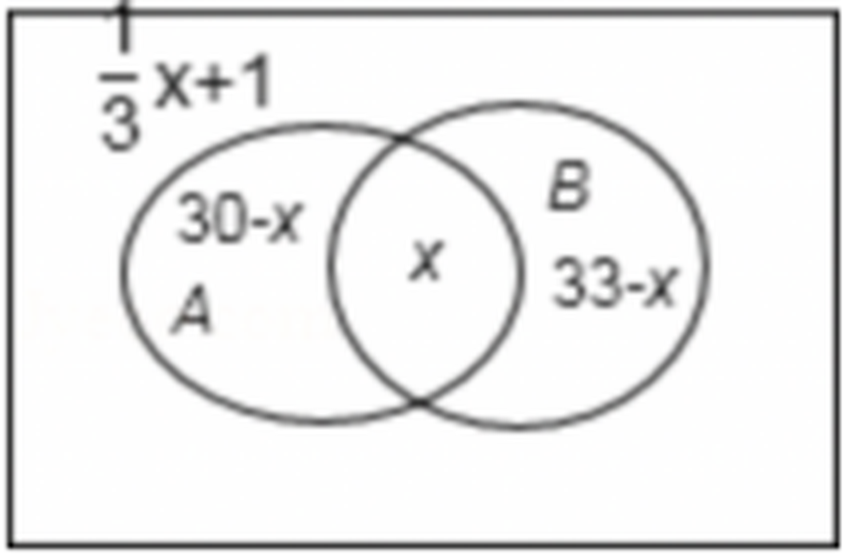
\includegraphics[width=0.30\textwidth]{figures/venn_AB_survey_50.png}
\end{center}

\ans{$21$}

\ifanswer
\solbegin
\step{由题意得赞成 $A$ 的人数 30，赞成 $B$ 的人数为 33，}
\step{设对 $A$、$B$ 都赞成的学生数为 $x$，则对 $A$、$B$ 都不赞成的学生数 $\dfrac{1}{3}x+1$，}
\step{如图得 $x+30-x+33-x+\dfrac{1}{3}x+1=50$，所以 $x=21$.}
\solend

\fi

\item 集合 $S=\{s\mid s=2n+1,n\in\Z\}$，$T=\{t\mid t=4n+1,n\in\Z\}$，则 $S$ \blankline[2.4em] $T$（填“$\subset$”“$\supset$”“$\subseteq$”或“$\supseteq$”）.

\ans{$S\supset T$}

\ifanswer
\solbegin
\step{对于 $S=\{s\mid s=2n+1,n\in\Z\}$ 为奇数，}
\step{而 $T=\{t\mid t=4n+1,n\in\Z\}$ 被 4 整除余 1 的奇数，所以 $S\supset T$.}
\solend

\fi

\item 已知集合 $A=\{x\mid -2<x<4\}$，$B=\{x\mid x^2-3ax+2a^2=0\}$，若 $A\cap B=B$，则实数 $a$ 的取值范围为 \blankline[4.4em].

\ans{$(-1,2)$}

\ifanswer
\solbegin
\step{因为 $A\cap B=B$，所以 $B\subseteq A$，}
\step{①当 $a=0$ 时，方程 $x^2-3ax+2a^2=0$ 的解为 $0$，$B\subseteq A$ 成立；}
\step{②当 $a\neq 0$ 时，方程 $x^2-3ax+2a^2=0$ 的解为 $2a$、$a$，}
\step{则 $-2<2a<4$ 且 $-2<a<4$，解得 $-1<a<2$ 且 $a\neq 0$；}
\step{综上所述，实数 $a$ 的取值范围为 $(-1,2)$.}
\solend

\fi

\item 当一个非空数集 $F$ 满足条件“若 $a$、$b\in F$，则 $a+b$、$a-b$、$ab\in F$，且当 $b\neq 0$ 时，$\dfrac{a}{b}\in F$”时，称 $F$ 为一个数域，以下四个关于数域的命题：

（1）$0$ 是任何数域的元素；（2）若数域 $F$ 有非零元素，则 $2026\in F$；

（3）集合 $P=\{x\mid x=3k,k\in\Z\}$ 为数域；（4）有理数集为数域；

其中，真命题的编号为 \blankline[4.4em]（写出所有真命题的编号）.

\ans{（1）（2）（4）}

\item 对于集合 $M$，定义函数 $f_M(x)=\begin{cases}-1,&x\in M\\ 1,&x\notin M\end{cases}$，对于两个集合 $M$、$N$，定义集合
$M\triangle N=\{x\mid f_M(x)\cdot f_N(x)=-1\}$，已知 $A=\{2,4,6,8,10\},B=\{1,2,4,8,16\}$，用 $|M|$ 表示有限集合 $M$ 中的元素个数，则对于任意集合 $M$，$|M\triangle A|+|M\triangle B|$ 的最小值为 \blankline[2.4em].

% 注：上面分段函数的第二行，原卷印作「1, $x\in M$」（两行都印 $x\in M$），与函数的定义矛盾，
%     本稿按文意订正为 $x\notin M$.
\ans{$4$}

\ifanswer
\solbegin
% 注：下面一行原卷印作「即 $M\triangle N\in\{x\mid x\in M\cup N\}$ 且 $x\in M\cap N$」，「$\in$」当为
%     「$=$」之误，且由 $f_M(x)f_N(x)=-1$ 应对应 $x\notin M\cap N$，本稿一并按文意订正.
\step{由 $M\triangle N$ 的定义得 $f_M(x)\cdot f_N(x)=-1$，}
\step{即 $M\triangle N=\{x\mid x\in M\cup N\text{ 且 }x\notin M\cap N\}$，}
\step{$|M\triangle A|+|M\triangle B|$ 要取得最小值，需满足 $A\cap B\subseteq M\subseteq A\cup B$，}
\step{此时 $|M\triangle A|+|M\triangle B|$ 的最小值为 $4$.}
\solend

\fi

\end{enumerate}

\bigsec{二、选择题}

\begin{enumerate}
\setcounter{enumi}{12}

\item 已知集合 $A=\{x\mid x=3m,m\in\N\}$，$B=\{x\mid x=3m+1,m\in\N\}$，$C=\{x\mid x=3m+2,m\in\N\}$，若 $a\in A$，$b\in B$，$c\in C$，则下列结论中可能成立的是\mbox{（\quad）}

\keepwithprev
A. $2021=a+b+c$\qquad B. $2021=abc$\qquad C. $2021=a+bc$\qquad D. $2021=a(b+c)$

\ans{C}

\ifanswer
\solbegin
\step{由题意设 $a=3m$，$b=3p+1$，$c=3n+2$，$m$、$p$、$n\in\N$，}
\step{则 $a+b+c=3m+3p+1+3n+2=3(m+p+n+1)$，}
\step{故 2021 不是 3 的整数倍，则 A 不可能；}
\step{$abc=3m(3p+1)(3n+2)$，同理 B 不可能；}
\step{$a+bc=3m+(3p+1)(3n+2)=3(m+3pn+2p+n)+2$，$2021=3\times 673+2$，}
\step{如取 $p=n=1$，则 $m=667$，即 $2021=3\times 667+4\times 5$，故 C 成立；}
\step{$a(b+c)=3m(3p+1+3n+2)=9m(p+n+1)$，同 A 可得 D 不可能.}
\step{故选 C.}
\solend

\fi

\item 设 $a$、$b$、$c$ 是实数，$x=a^2-2b+\dfrac{\pi}{3}$，$y=b^2-2c+\dfrac{\pi}{6}$，$z=c^2-2a+\dfrac{\pi}{2}$，则 $x$、$y$、$z$ 中至少有一个值\mbox{（\quad）}

\keepwithprev
A. 大于 $0$\qquad B. 等于 $0$\qquad C. 不大于 $0$\qquad D. 小于 $0$

\ans{A}

\ifanswer
\solbegin
\step{因为 $x+y+z=a^2-2b+\dfrac{\pi}{3}+b^2-2c+\dfrac{\pi}{6}+c^2-2a+\dfrac{\pi}{2}=(a-1)^2+(b-1)^2+(c-1)^2+\pi-3>0$，}
\step{假设 $x$、$y$、$z$ 都不大于 $0$，即 $x\leqslant 0$，$y\leqslant 0$，$z\leqslant 0$，}
\step{由同向不等式的可加性得 $x+y+z\leqslant 0$①，又 $x+y+z>0$ 与①式矛盾.}
\step{所以假设不成立，即原命题的结论 $x$、$y$、$z$ 中至少有一个大于 $0$. 故选 A.}
\solend

\fi

\item 命题“存在一个无理数，它的平方是有理数”的否定是\mbox{（\quad）}

\keepwithprev
A. 任意一个有理数，它的平方是有理数

B. 任意一个无理数，它的平方不是有理数

C. 存在一个有理数，它的平方是有理数

D. 存在一个无理数，它的平方不是有理数

\ans{B}

\ifanswer
\solbegin
\step{否定是任意一个无理数，它的平方不是有理数，故选 B.}
\solend

\fi

\item 设集合 $P_1=\{x\mid x^2+ax+1>0\}$，$P_2=\{x\mid x^2+ax+2>0\}$，$Q_1=\{x\mid x^2+x+b>0\}$，$Q_2=\{x\mid x^2+2x+b>0\}$，其中 $a$、$b\in\R$，下列说法正确的是\mbox{（\quad）}

\keepwithprev
A. 对任意 $a$，$P_1$ 是 $P_2$ 的子集，对任意 $b$，$Q_1$ 不是 $Q_2$ 的子集

B. 对任意 $a$，$P_1$ 是 $P_2$ 的子集，存在 $b$，使得 $Q_1$ 是 $Q_2$ 的子集

C. 对任意 $a$，使得 $P_1$ 不是 $P_2$ 的子集，对任意 $b$，$Q_1$ 不是 $Q_2$ 的子集

D. 对任意 $a$，使得 $P_1$ 不是 $P_2$ 的子集，存在 $b$，使得 $Q_1$ 不是 $Q_2$ 的子集

\ans{B}

\ifanswer
\solbegin
\step{对于集合 $P_1=\{x\mid x^2+ax+1>0\}$，$P_2=\{x\mid x^2+ax+2>0\}$，}
\step{得当 $m\in P_1$，即 $m^2+am+1>0$，得 $m^2+am+2>0$，}
\step{即有 $m\in P_2$，得对任意 $a$，$P_1$ 是 $P_2$ 的子集；}
\step{当 $b=5$ 时，$Q_1=\{x\mid x^2+x+5>0\}=\R$，$Q_2=\{x\mid x^2+2x+5>0\}=\R$，}
\step{得 $Q_1$ 是 $Q_2$ 的子集，故 A 错误，B 正确；}
\step{当 $b=1$ 时，$Q_1=\{x\mid x^2+x+1>0\}=\R$，}
\step{$Q_2=\{x\mid x^2+2x+1>0\}=\{x\mid x\neq -1\text{ 且 }x\in\R\}$，得 $Q_1$ 不是 $Q_2$ 的子集.}
\step{综上，对任意 $a$，$P_1$ 是 $P_2$ 的子集，存在 $b$，使得 $Q_1$ 是 $Q_2$ 的子集，}
\step{故 C 错误，D 错误.}
\step{故选 B.}
\solend

\fi

\end{enumerate}

\bigsec{三、解答题}

\begin{enumerate}
\setcounter{enumi}{16}

\item 已知集合 $A=\{x\mid 0<x-a\leqslant 5\}$，$B=\left\{x\mid -\dfrac{a}{2}<x\leqslant 6\right\}$.

\begin{enumerate}[label=(\arabic*)]
\item 若 $A\subseteq B$，求 $a$ 的取值范围.
\item 集合 $A$ 与 $B$ 能否相等？若能，求出 $a$ 的值，若不能，请说明理由.
\end{enumerate}

\ans{（1）$0\leqslant a\leqslant 1$；（2）不能，$a\in\varnothing$}

\ifanswer
\solbegin
\stepm{（1）}{由于 $A\subseteq B$，所以 $a+5\leqslant 6$，且 $-\dfrac{a}{2}\leqslant a$，解得 $0\leqslant a\leqslant 1$；}
\stepm{（2）}{$A=B$ 时，$a+5=6$，$-\dfrac{a}{2}=a$，解得 $a\in\varnothing$.}
\solend

\fi

\ansspace[6]

\item 已知 $\alpha:2x+m<0$，$\beta:-1<x<3$.

\begin{enumerate}[label=(\arabic*)]
\item 是否存在实数 $m$，使得 $\alpha$ 是 $\beta$ 的充分条件？若存在，求出实数 $m$ 的取值范围；
\item 是否存在实数 $m$，使得 $\alpha$ 是 $\beta$ 的必要条件？若存在，求出实数 $m$ 的取值范围.
\end{enumerate}

\ans{（1）不存在；（2）存在，$m\leqslant -6$}

\ansspace[6]

\item 已知 $\triangle ABC$ 的三边长分别为 $a,b,c$，证明：

\begin{enumerate}[label=(\arabic*)]
\item “$A=90^\circ$”是“关于 $x$ 的方程 $x^2+2ax+b^2=0$ 与 $x^2+2cx-b^2=0$ 有公共实根”的充分条件；
\item “$a=c$”是“关于 $x$ 的方程 $x^2+2ax+b^2=0$ 与 $x^2+2cx-b^2=0$ 没有公共实根”的充分非必要条件.
\end{enumerate}

\ans{（1）略；（2）略}

\ansspace[8]

\item 已知集合 $A$ 包含有 $n(n\in\N^*)$ 个元素，$A^+=\{x+y\mid x\text{、}y\in A\}$.

\begin{enumerate}[label=(\arabic*)]
\item 若 $A=\{0,1,2\}$，写出 $A^+$；
\item % 注：原卷此处印作「写出一个 $A^+$，使得 $A=A^+$」——$A$ 未给定，该问无法作答，
      %     与下方【解析】「取 $A=\{0\}$」不符，本稿按文意订正为「写出一个 $A$」.
      写出一个 $A$，使得 $A=A^+$；
\item 当 $n=4$ 时，是否存在集合 $A$，使得 $A^+=\{2,3,5,6,7,8,10\}$？若存在，求出此时的集合 $A$，若不存在，请说明理由.
\end{enumerate}

\ans{（1）$\{0,1,2,3,4\}$；（2）$A=\{0\}$；（3）不存在}

\ifanswer
\solbegin
\stepm{（1）}{由题意得 $0+0=0$，$0+1=1$，$0+2=2$，$1+1=2$，$1+2=3$，$2+2=4$ 都是 $A^+$ 中的元素，故 $A^+=\{0,1,2,3,4\}$；}
\stepm{（2）}{取 $A=\{0\}$，此时 $A^+=\{x+y\mid x\text{、}y\in A\}=\{0\}$，符合 $A=A^+$；}
\stepm{（3）}{当 $n=4$ 时，不存在集合 $A$，使得 $A^+=\{2,3,5,6,7,8,10\}$，理由如下：}
\step{假设存在 $A=\{a,b,c,d\}$，且 $a<b<c<d$，}
\step{则 $2a<a+b<a+c<b+c<b+d<c+d<2d$，}
\step{故 $2a,a+b,a+c,b+c,b+d,c+d,2d$ 为 $A^+$ 中 7 个不同的元素，}
\step{则 $2a=2$，$a+b=3$，$a+c=5$，$b+c=6$，$b+d=7$，$c+d=8$，$2d=10$，}
\step{解得 $a=1$，$b=2$，$c=4$，$d=5$，}
\step{此时 $c+d=9\in A^+$ 与 $9\notin A^+$ 矛盾，故假设不成立，}
\step{即不存在这样的集合 $A$.}
\solend

\fi

\ansspace[8]

% 压轴题：在其 \item 前先量一下版面，本页剩余高度不足 7cm 就另起一页。
\ansneed{7cm}

\item 已知集合 $A$ 为非空数集，对于集合 $A$，对 $A$ 中任意两个不同元素相加得到的和取绝对值，将这些绝对值重新组成一个新的集合，对于这一过程，我们定义为“自相加”，重新组成的集合叫做“集合 $A$ 的 1 次自相加集合”，再进行 $n-1$ 次“自相加”操作，组成的集合叫做“集合 $A$ 的 $n$ 次自相加集合”. 若集合 $A$ 的任意 $k$ 次自相加集合都不相等，则称集合 $A$ 为“完美自相加集合”，同理，我们可以定义出“$A$ 的 1 次自相减集合”，集合 $A$ 的 1 次自相加集合和 1 次自相减集合分别可表示为：$A^+=\{x\mid x=|a+b|,\ a\text{、}b\in A\}$，$A^-=\{x\mid x=|a-b|,\ a\text{、}b\in A\}$.

\begin{enumerate}[label=(\arabic*)]
\item 已知有两个集合，集合 $B=\{1,2,3,4\}$，集合 $C=\{k\mid k=2n+1,n\in\Z\}$，判断集合 $B$ 和集合 $C$ 是否是完美自相加集合，并说明理由；
\item 对（1）中的集合 $B$ 进行 11 次自相加操作后，求：集合 $B$ 的 11 次自相加集合的元素个数；
\item 若 $0\leqslant n\leqslant 2025$ 且 $n\in\N$，集合 $A=\{x\mid n\leqslant x\leqslant 2025,x\in\N\}$，$A^+\cap A^-=\varnothing$，求：$n$ 的最小值.
\end{enumerate}

\ans{（1）$B$ 是完美自相加集合，$C$ 不是完美自相加集合；（2）$2051$；（3）$675$}

\ifanswer
\solbegin
\stepm{（1）}{$B$ 是完美自相加集合，$C$ 不是完美自相加集合，}
\step{理由如下：因为集合 $B=\{1,2,3,4\}$，所以 $B^+=\{3,4,5,6,7\}$，}
\step{由此可得集合自相加后，}
\step{新的集合中最小的元素为自相加之前的集合中的最小两个元素之和，}
\step{所以显然集合 $B=\{1,2,3,4\}$ 的最小两个元素为 $1$，$2$，}
\step{所以 $B^+$ 中的最小元素为 $1+2=3$，}
\step{同理，2 次自相加后得到的集合中的最小元素是 $3+4=7$.}
\step{依照这样的规律，对集合 $B=\{1,2,3,4\}$ 进行任意次自相加操作后，}
\step{最小值总在变大，故不可能有相等集合，所以 $B$ 是完美自相加集合；}
\step{因为集合 $C=\{k\mid k=2n+1,n\in\Z\}$ 表示所有奇数构成的集合，}
\step{任何两个奇数相加的和都是偶数，}
\step{所以 $C^+=\{k\mid k=2n,n\in\Z\}$ 为所有偶数构成集合；}
\step{所以对 $C^+=\{k\mid k=2n,n\in\Z\}$ 再进行一次自相加操作，}
\step{因为任意两个偶数相加的和还是偶数，}
\step{所以后面集合不管进行多少次相加都与 $C^+=\{k\mid k=2n,n\in\Z\}$ 相同；}
\step{故 $C$ 不是完美自相加集合.}
\stepm{（2）}{由自相加性质得，对于集合 $B=\{1,2,3,4\}$，进行一次自相加，}
\step{得到集合的最小值必然是原来集合的两个最小元素值之和，}
\step{得到的最大值必然为原来集合的两个最大元素值之和，}
\step{且中间必然是连续的整数元素；}
\step{所以对集合 $B=\{1,2,3,4\}$ 进行 1 次自相加之后，}
\step{得到的集合最小两个元素为 $3$，$4$，最大的两个元素为 $6$，$7$；}
\step{进行第 2 次自相加，得到的集合最小两个元素为 $7$，$8$，}
\step{最大的两个元素为 $12$，$13$；}
\step{进行第 3 次自相加，得到的集合最小两个元素为 $15$，$16$，}
\step{最大的两个元素为 $24$，$25$；}
\step{进行第 4 次自相加，得到的集合最小两个元素为 $31$，$32$，}
\step{最大的两个元素为 $48$，$49$；}
\step{进行第 5 次自相加，得到的集合最小两个元素为 $63$，$64$，}
\step{最大的两个元素为 $96$，$97$；}
\step{进行第 6 次自相加，得到的集合最小两个元素为 $127$，$128$，}
\step{最大的两个元素为 $192$，$193$；}
\step{进行第 7 次自相加，得到的集合最小两个元素为 $255$，$256$，}
\step{最大的两个元素为 $384$，$385$；}
\step{进行第 8 次自相加，得到的集合最小两个元素为 $511$，$512$，}
\step{最大的两个元素为 $768$，$769$；}
\step{进行第 9 次自相加，得到的集合最小两个元素为 $1023$，$1024$，}
\step{最大的两个元素为 $1536$，$1537$；}
\step{进行第 10 次自相加，得到的集合最小两个元素为 $2047$，$2048$，}
\step{最大的两个元素为 $3072$，$3073$；}
\step{进行第 11 次自相加，得到的集合最小两个元素为 $4095$，$4096$，}
\step{最大的两个元素为 $6144$，$6145$；}
\step{因为集合 $B$ 的 $n$ 次自相加集合中的元素都是连续的整数，}
\step{所以集合 $B$ 进行 11 次自相加操作后的元素个数为 $6145-4095+1=2051$.}
\stepm{（3）}{因为 $0\leqslant n\leqslant 2025$ 且 $n\in\N$，集合 $A=\{x\mid n\leqslant x\leqslant 2025,x\in\N\}$，}
\step{所以 $A^+=\{x\mid 2n+1\leqslant x\leqslant 4049,x\in\N\}$，}
\step{$A^-=\{x\mid 1\leqslant x\leqslant 2025-n,x\in\N\}$，}
\step{要使 $A^+\cap A^-=\varnothing$，须使 $2n+1>2025-n$，所以 $n>\dfrac{2024}{3}=674\dfrac{2}{3}$，}
\step{又 $n\in\N$，故 $n$ 的最小值为 $675$.}
\solend

\fi

% 压轴题：其后已无内容，故作答区全用可丢弃胶水（\ansspace*）。
\ansspace*[12]

\end{enumerate}

\end{document}
"
%
% 原始材料是微信公众号图文（公众号「魔都数学加油站」），正文为 10 张 PNG 页（1080×1527）。
% 原文本身就是一份**讲评版**——题目下方直接印出【答案】或【解析】，选择题的答案印在解析末句
% 「故选 X」里。试题文字、答案与解析均照原卷录入（订正处见下），卷面上的粉色斜水印
% 「魔都数学加油站」属水印，未录入。
%
% 与原卷的排版差异（均已在 README「说明」中交代）：
%   ① 原文自**第 3 题**起（第 1、2 题未在该文中发布），故本稿题号亦自 3 起；
%   ② 原卷本就印有「一、填空题」「二、选择题」「三、解答题」三节标题（分别在原图 00/02/04.png
%      上，逐页核对过），本稿照原卷分节，只把标题改排成全稿统一的「大节标题」样式；
%   ③ 原卷填空、选择的答案直接印在题目下方（选择题只在解析末句「故选 X」中给出），本稿统一改为
%      试卷版隐去、答案版以【答案】给出，选择题的括注一律改排「\mbox{（\quad）}」并把答案移到选项之后，
%      使两版彻底分离；
%   ④ 原卷的集合符号大小写混用：第 3 题题干的实数集印成**粗体** $\mathbf{R}$，第 16 题题干与
%      第 16 题解析的印成正体 $R$；自然数集 $N$、整数集 $Z$ 一律正体。本稿按全稿惯例统一写作
%      $\R$、$\N$、$\Z$；
%   ⑤ 原卷未印副标题，本稿按全稿惯例补出副标题「集合与常用逻辑用语」；
%   ⑥ 原卷解答题子问编号为「（1）（2）」，本稿用嵌套 enumerate 排成同一形态；原卷第 15 题的
%      D 选项因原页翻页被截到下一页首页，本稿自然连排；
%   ⑦ 原卷解答题未留作答空间（讲评稿通篇是答案），本稿逐题补出书写留白，仅试卷版显示；
%   ⑧ 第 21 题题干里 $A^+$、$A^-$ 的定义含绝对值号（原卷作 $\{x\mid x=|a+b|,\ a\text{、}b\in A\}$
%      与 $\{x\mid x=|a-b|,\ a\text{、}b\in A\}$），本稿照原卷录入；2026-09-15 回原图逐处放大复核
%      时发现曾漏抄两处绝对值号、并把分隔逗号误写成 $\mid$，已按原卷订正（见 README 专记）。
%
% 原卷笔误三处（均已放大到能看清字形后核对，本稿按文意订正，并在 README 中写明原委）：
%   ① 第 12 题题干的分段函数 $f_M(x)$ 原卷两行都印作「$x\in M$」（$-1$ 与 $1$ 都取在 $M$ 上），
%      与「函数」的定义直接矛盾（$M$ 上无法同时取两个值），按文意订正第二行为 $x\notin M$；
%   ② 第 12 题【解析】首行原卷印「即 $M\triangle N\in\{x\mid x\in M\cup N\}$ 且 $x\in M\cap N$」，
%      其中「$\in$」当为「$=$」之误；且由 $f_M(x)f_N(x)=-1$ 应对应 $x\notin M\cap N$（原卷印作
%      $x\in M\cap N$，与上一行刚写出的对称差的定义相矛盾），本稿一并订正；
%   ③ 第 20 题(2)原卷印「写出一个 $A^+$，使得 $A=A^+$」——$A$ 未给定，该问无法作答，与紧接的
%      【解析】「取 $A=\{0\}$，此时 $A^+=\{0\}$，符合 $A=A^+$」不符，本稿按文意订正为
%      「写出一个 $A$，使得 $A=A^+$」.
%
% 原卷存疑一处（无法确证原意，本稿照抄原卷、未改）：
%   ① 第 5 题 ④ 原卷题干印 $S=\{x\mid |x|\leqslant\sqrt{3},x\in N\}$（该字母与 ③ 中的 $Z$
%      字形明显不同，$Z$ 有上下两横，已放大比对确认），而【解析】印「因为 $S=\{-1,0,1\}$」——
%      按 $x\in N$ 应为 $S=\{0,1\}$（或 $\{1\}$），题干与解析的口径不一致；但无论取哪一口径，
%      ④ 都是 $M$ 的子集、本题结论（填④）不变，故题干与解析均照抄原卷，未改。

\documentclass[a4paper,11pt]{article}
\usepackage{common}

\begin{document}

\examtitlest{2026--2027 年七宝中学高一上周末作业 2}{集合与常用逻辑用语}

\bigsec{一、填空题}

\begin{enumerate}
\setcounter{enumi}{2}

\item 已知 $a,x\in\R$，则“$x\in\{-a,a\}$”是“$|x|=a$”的 \blankline[4.4em] 条件.

\ans{必要不充分}

\item 设全集为 $U$，$A\subseteq U$，$B\subseteq U$，则“$A\subset B$”是“$\overline{B}\subset\overline{A}$”的 \blankline[4.4em] 条件.

\ans{充要}

\item 已知集合 $M=\{x\mid -\sqrt{5}<x<\sqrt{3},x\in\Z\}$，则下列集合是集合 $M$ 的子集的是 \blankline[4.4em]（填序号）.

① $P=\{-3,0,1\}$；② $Q=\{-1,0,1,2\}$；③ $R=\{y\mid -\pi<y<-1,y\in\Z\}$；

④ $S=\{x\mid |x|\leqslant\sqrt{3},x\in\N\}$.

\ans{④}

\ifanswer
\solbegin
\step{由已知得集合 $M=\{-2,-1,0,1\}$，}
\step{所以由子集的定义得选项①错误，②错误，}
\step{因为 $R=\{-3,-2\}$，所以集合 $R$ 不表示集合 $M$ 的子集，③错误，}
\step{因为 $S=\{-1,0,1\}$，所以是集合 $M$ 的子集，故正确.}
\step{故是集合 $M$ 的子集的是④.}
\solend

\fi

\item 已知 $x\in\R$，用反证法证明命题“若 $x^2-7x+10<0$，则 $2<x<5$”时，应该假设 \blankline[5em].

\ans{$x\leqslant 2$ 或 $x\geqslant 5$}

\item 设 $a_1,b_1,c_1,a_2,b_2,c_2$ 均为非零实数，方程 $a_1x^2+b_1x+c_1=0$ 和 $a_2x^2+b_2x+c_2=0$ 的解集分别为 $M$ 和 $N$，那么“$\dfrac{a_1}{a_2}=\dfrac{b_1}{b_2}=\dfrac{c_1}{c_2}$”是“$M=N$”的 \blankline[4.4em] 条件.

（填“充分非必要”、“必要非充分”、“充要”、或“既非充分又非必要”）

\ans{充分非必要}

\ifanswer
\solbegin
\step{$\dfrac{a_1}{a_2}=\dfrac{b_1}{b_2}=\dfrac{c_1}{c_2}$ 能推出 $M=N$，}
\step{若 $M=N=\varnothing$ 推不出 $\dfrac{a_1}{a_2}=\dfrac{b_1}{b_2}=\dfrac{c_1}{c_2}$，}
\step{所以“$\dfrac{a_1}{a_2}=\dfrac{b_1}{b_2}=\dfrac{c_1}{c_2}$”是“$M=N$”的“充分非必要”条件.}
\solend

\fi

\item 向 50 名学生调查对 $A$、$B$ 两事件的态度，有如下结果赞成 $A$ 的人数是全体的五分之三，其余的不赞成，赞成 $B$ 的比赞成 $A$ 的多 3 人，其余的不赞成；另外，对 $A$、$B$ 都不赞成的学生数比对 $A$、$B$ 都赞成的学生数的三分之一多 1 人. 则对 $A$、$B$ 都赞成的学生有 \blankline[2.4em] 人.

\begin{center}
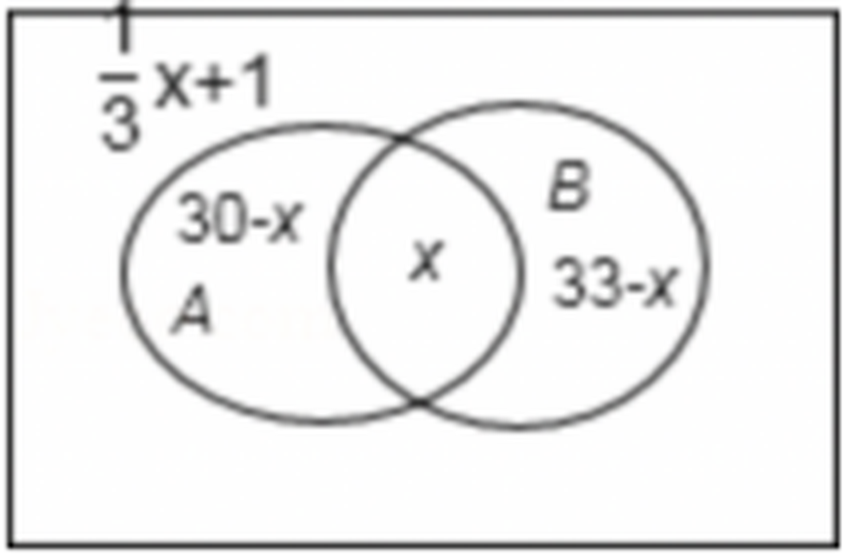
\includegraphics[width=0.30\textwidth]{figures/venn_AB_survey_50.png}
\end{center}

\ans{$21$}

\ifanswer
\solbegin
\step{由题意得赞成 $A$ 的人数 30，赞成 $B$ 的人数为 33，}
\step{设对 $A$、$B$ 都赞成的学生数为 $x$，则对 $A$、$B$ 都不赞成的学生数 $\dfrac{1}{3}x+1$，}
\step{如图得 $x+30-x+33-x+\dfrac{1}{3}x+1=50$，所以 $x=21$.}
\solend

\fi

\item 集合 $S=\{s\mid s=2n+1,n\in\Z\}$，$T=\{t\mid t=4n+1,n\in\Z\}$，则 $S$ \blankline[2.4em] $T$（填“$\subset$”“$\supset$”“$\subseteq$”或“$\supseteq$”）.

\ans{$S\supset T$}

\ifanswer
\solbegin
\step{对于 $S=\{s\mid s=2n+1,n\in\Z\}$ 为奇数，}
\step{而 $T=\{t\mid t=4n+1,n\in\Z\}$ 被 4 整除余 1 的奇数，所以 $S\supset T$.}
\solend

\fi

\item 已知集合 $A=\{x\mid -2<x<4\}$，$B=\{x\mid x^2-3ax+2a^2=0\}$，若 $A\cap B=B$，则实数 $a$ 的取值范围为 \blankline[4.4em].

\ans{$(-1,2)$}

\ifanswer
\solbegin
\step{因为 $A\cap B=B$，所以 $B\subseteq A$，}
\step{①当 $a=0$ 时，方程 $x^2-3ax+2a^2=0$ 的解为 $0$，$B\subseteq A$ 成立；}
\step{②当 $a\neq 0$ 时，方程 $x^2-3ax+2a^2=0$ 的解为 $2a$、$a$，}
\step{则 $-2<2a<4$ 且 $-2<a<4$，解得 $-1<a<2$ 且 $a\neq 0$；}
\step{综上所述，实数 $a$ 的取值范围为 $(-1,2)$.}
\solend

\fi

\item 当一个非空数集 $F$ 满足条件“若 $a$、$b\in F$，则 $a+b$、$a-b$、$ab\in F$，且当 $b\neq 0$ 时，$\dfrac{a}{b}\in F$”时，称 $F$ 为一个数域，以下四个关于数域的命题：

（1）$0$ 是任何数域的元素；（2）若数域 $F$ 有非零元素，则 $2026\in F$；

（3）集合 $P=\{x\mid x=3k,k\in\Z\}$ 为数域；（4）有理数集为数域；

其中，真命题的编号为 \blankline[4.4em]（写出所有真命题的编号）.

\ans{（1）（2）（4）}

\item 对于集合 $M$，定义函数 $f_M(x)=\begin{cases}-1,&x\in M\\ 1,&x\notin M\end{cases}$，对于两个集合 $M$、$N$，定义集合
$M\triangle N=\{x\mid f_M(x)\cdot f_N(x)=-1\}$，已知 $A=\{2,4,6,8,10\},B=\{1,2,4,8,16\}$，用 $|M|$ 表示有限集合 $M$ 中的元素个数，则对于任意集合 $M$，$|M\triangle A|+|M\triangle B|$ 的最小值为 \blankline[2.4em].

% 注：上面分段函数的第二行，原卷印作「1, $x\in M$」（两行都印 $x\in M$），与函数的定义矛盾，
%     本稿按文意订正为 $x\notin M$.
\ans{$4$}

\ifanswer
\solbegin
% 注：下面一行原卷印作「即 $M\triangle N\in\{x\mid x\in M\cup N\}$ 且 $x\in M\cap N$」，「$\in$」当为
%     「$=$」之误，且由 $f_M(x)f_N(x)=-1$ 应对应 $x\notin M\cap N$，本稿一并按文意订正.
\step{由 $M\triangle N$ 的定义得 $f_M(x)\cdot f_N(x)=-1$，}
\step{即 $M\triangle N=\{x\mid x\in M\cup N\text{ 且 }x\notin M\cap N\}$，}
\step{$|M\triangle A|+|M\triangle B|$ 要取得最小值，需满足 $A\cap B\subseteq M\subseteq A\cup B$，}
\step{此时 $|M\triangle A|+|M\triangle B|$ 的最小值为 $4$.}
\solend

\fi

\end{enumerate}

\bigsec{二、选择题}

\begin{enumerate}
\setcounter{enumi}{12}

\item 已知集合 $A=\{x\mid x=3m,m\in\N\}$，$B=\{x\mid x=3m+1,m\in\N\}$，$C=\{x\mid x=3m+2,m\in\N\}$，若 $a\in A$，$b\in B$，$c\in C$，则下列结论中可能成立的是\mbox{（\quad）}

\keepwithprev
A. $2021=a+b+c$\qquad B. $2021=abc$\qquad C. $2021=a+bc$\qquad D. $2021=a(b+c)$

\ans{C}

\ifanswer
\solbegin
\step{由题意设 $a=3m$，$b=3p+1$，$c=3n+2$，$m$、$p$、$n\in\N$，}
\step{则 $a+b+c=3m+3p+1+3n+2=3(m+p+n+1)$，}
\step{故 2021 不是 3 的整数倍，则 A 不可能；}
\step{$abc=3m(3p+1)(3n+2)$，同理 B 不可能；}
\step{$a+bc=3m+(3p+1)(3n+2)=3(m+3pn+2p+n)+2$，$2021=3\times 673+2$，}
\step{如取 $p=n=1$，则 $m=667$，即 $2021=3\times 667+4\times 5$，故 C 成立；}
\step{$a(b+c)=3m(3p+1+3n+2)=9m(p+n+1)$，同 A 可得 D 不可能.}
\step{故选 C.}
\solend

\fi

\item 设 $a$、$b$、$c$ 是实数，$x=a^2-2b+\dfrac{\pi}{3}$，$y=b^2-2c+\dfrac{\pi}{6}$，$z=c^2-2a+\dfrac{\pi}{2}$，则 $x$、$y$、$z$ 中至少有一个值\mbox{（\quad）}

\keepwithprev
A. 大于 $0$\qquad B. 等于 $0$\qquad C. 不大于 $0$\qquad D. 小于 $0$

\ans{A}

\ifanswer
\solbegin
\step{因为 $x+y+z=a^2-2b+\dfrac{\pi}{3}+b^2-2c+\dfrac{\pi}{6}+c^2-2a+\dfrac{\pi}{2}=(a-1)^2+(b-1)^2+(c-1)^2+\pi-3>0$，}
\step{假设 $x$、$y$、$z$ 都不大于 $0$，即 $x\leqslant 0$，$y\leqslant 0$，$z\leqslant 0$，}
\step{由同向不等式的可加性得 $x+y+z\leqslant 0$①，又 $x+y+z>0$ 与①式矛盾.}
\step{所以假设不成立，即原命题的结论 $x$、$y$、$z$ 中至少有一个大于 $0$. 故选 A.}
\solend

\fi

\item 命题“存在一个无理数，它的平方是有理数”的否定是\mbox{（\quad）}

\keepwithprev
A. 任意一个有理数，它的平方是有理数

B. 任意一个无理数，它的平方不是有理数

C. 存在一个有理数，它的平方是有理数

D. 存在一个无理数，它的平方不是有理数

\ans{B}

\ifanswer
\solbegin
\step{否定是任意一个无理数，它的平方不是有理数，故选 B.}
\solend

\fi

\item 设集合 $P_1=\{x\mid x^2+ax+1>0\}$，$P_2=\{x\mid x^2+ax+2>0\}$，$Q_1=\{x\mid x^2+x+b>0\}$，$Q_2=\{x\mid x^2+2x+b>0\}$，其中 $a$、$b\in\R$，下列说法正确的是\mbox{（\quad）}

\keepwithprev
A. 对任意 $a$，$P_1$ 是 $P_2$ 的子集，对任意 $b$，$Q_1$ 不是 $Q_2$ 的子集

B. 对任意 $a$，$P_1$ 是 $P_2$ 的子集，存在 $b$，使得 $Q_1$ 是 $Q_2$ 的子集

C. 对任意 $a$，使得 $P_1$ 不是 $P_2$ 的子集，对任意 $b$，$Q_1$ 不是 $Q_2$ 的子集

D. 对任意 $a$，使得 $P_1$ 不是 $P_2$ 的子集，存在 $b$，使得 $Q_1$ 不是 $Q_2$ 的子集

\ans{B}

\ifanswer
\solbegin
\step{对于集合 $P_1=\{x\mid x^2+ax+1>0\}$，$P_2=\{x\mid x^2+ax+2>0\}$，}
\step{得当 $m\in P_1$，即 $m^2+am+1>0$，得 $m^2+am+2>0$，}
\step{即有 $m\in P_2$，得对任意 $a$，$P_1$ 是 $P_2$ 的子集；}
\step{当 $b=5$ 时，$Q_1=\{x\mid x^2+x+5>0\}=\R$，$Q_2=\{x\mid x^2+2x+5>0\}=\R$，}
\step{得 $Q_1$ 是 $Q_2$ 的子集，故 A 错误，B 正确；}
\step{当 $b=1$ 时，$Q_1=\{x\mid x^2+x+1>0\}=\R$，}
\step{$Q_2=\{x\mid x^2+2x+1>0\}=\{x\mid x\neq -1\text{ 且 }x\in\R\}$，得 $Q_1$ 不是 $Q_2$ 的子集.}
\step{综上，对任意 $a$，$P_1$ 是 $P_2$ 的子集，存在 $b$，使得 $Q_1$ 是 $Q_2$ 的子集，}
\step{故 C 错误，D 错误.}
\step{故选 B.}
\solend

\fi

\end{enumerate}

\bigsec{三、解答题}

\begin{enumerate}
\setcounter{enumi}{16}

\item 已知集合 $A=\{x\mid 0<x-a\leqslant 5\}$，$B=\left\{x\mid -\dfrac{a}{2}<x\leqslant 6\right\}$.

\begin{enumerate}[label=(\arabic*)]
\item 若 $A\subseteq B$，求 $a$ 的取值范围.
\item 集合 $A$ 与 $B$ 能否相等？若能，求出 $a$ 的值，若不能，请说明理由.
\end{enumerate}

\ans{（1）$0\leqslant a\leqslant 1$；（2）不能，$a\in\varnothing$}

\ifanswer
\solbegin
\stepm{（1）}{由于 $A\subseteq B$，所以 $a+5\leqslant 6$，且 $-\dfrac{a}{2}\leqslant a$，解得 $0\leqslant a\leqslant 1$；}
\stepm{（2）}{$A=B$ 时，$a+5=6$，$-\dfrac{a}{2}=a$，解得 $a\in\varnothing$.}
\solend

\fi

\ansspace[6]

\item 已知 $\alpha:2x+m<0$，$\beta:-1<x<3$.

\begin{enumerate}[label=(\arabic*)]
\item 是否存在实数 $m$，使得 $\alpha$ 是 $\beta$ 的充分条件？若存在，求出实数 $m$ 的取值范围；
\item 是否存在实数 $m$，使得 $\alpha$ 是 $\beta$ 的必要条件？若存在，求出实数 $m$ 的取值范围.
\end{enumerate}

\ans{（1）不存在；（2）存在，$m\leqslant -6$}

\ansspace[6]

\item 已知 $\triangle ABC$ 的三边长分别为 $a,b,c$，证明：

\begin{enumerate}[label=(\arabic*)]
\item “$A=90^\circ$”是“关于 $x$ 的方程 $x^2+2ax+b^2=0$ 与 $x^2+2cx-b^2=0$ 有公共实根”的充分条件；
\item “$a=c$”是“关于 $x$ 的方程 $x^2+2ax+b^2=0$ 与 $x^2+2cx-b^2=0$ 没有公共实根”的充分非必要条件.
\end{enumerate}

\ans{（1）略；（2）略}

\ansspace[8]

\item 已知集合 $A$ 包含有 $n(n\in\N^*)$ 个元素，$A^+=\{x+y\mid x\text{、}y\in A\}$.

\begin{enumerate}[label=(\arabic*)]
\item 若 $A=\{0,1,2\}$，写出 $A^+$；
\item % 注：原卷此处印作「写出一个 $A^+$，使得 $A=A^+$」——$A$ 未给定，该问无法作答，
      %     与下方【解析】「取 $A=\{0\}$」不符，本稿按文意订正为「写出一个 $A$」.
      写出一个 $A$，使得 $A=A^+$；
\item 当 $n=4$ 时，是否存在集合 $A$，使得 $A^+=\{2,3,5,6,7,8,10\}$？若存在，求出此时的集合 $A$，若不存在，请说明理由.
\end{enumerate}

\ans{（1）$\{0,1,2,3,4\}$；（2）$A=\{0\}$；（3）不存在}

\ifanswer
\solbegin
\stepm{（1）}{由题意得 $0+0=0$，$0+1=1$，$0+2=2$，$1+1=2$，$1+2=3$，$2+2=4$ 都是 $A^+$ 中的元素，故 $A^+=\{0,1,2,3,4\}$；}
\stepm{（2）}{取 $A=\{0\}$，此时 $A^+=\{x+y\mid x\text{、}y\in A\}=\{0\}$，符合 $A=A^+$；}
\stepm{（3）}{当 $n=4$ 时，不存在集合 $A$，使得 $A^+=\{2,3,5,6,7,8,10\}$，理由如下：}
\step{假设存在 $A=\{a,b,c,d\}$，且 $a<b<c<d$，}
\step{则 $2a<a+b<a+c<b+c<b+d<c+d<2d$，}
\step{故 $2a,a+b,a+c,b+c,b+d,c+d,2d$ 为 $A^+$ 中 7 个不同的元素，}
\step{则 $2a=2$，$a+b=3$，$a+c=5$，$b+c=6$，$b+d=7$，$c+d=8$，$2d=10$，}
\step{解得 $a=1$，$b=2$，$c=4$，$d=5$，}
\step{此时 $c+d=9\in A^+$ 与 $9\notin A^+$ 矛盾，故假设不成立，}
\step{即不存在这样的集合 $A$.}
\solend

\fi

\ansspace[8]

% 压轴题：在其 \item 前先量一下版面，本页剩余高度不足 7cm 就另起一页。
\ansneed{7cm}

\item 已知集合 $A$ 为非空数集，对于集合 $A$，对 $A$ 中任意两个不同元素相加得到的和取绝对值，将这些绝对值重新组成一个新的集合，对于这一过程，我们定义为“自相加”，重新组成的集合叫做“集合 $A$ 的 1 次自相加集合”，再进行 $n-1$ 次“自相加”操作，组成的集合叫做“集合 $A$ 的 $n$ 次自相加集合”. 若集合 $A$ 的任意 $k$ 次自相加集合都不相等，则称集合 $A$ 为“完美自相加集合”，同理，我们可以定义出“$A$ 的 1 次自相减集合”，集合 $A$ 的 1 次自相加集合和 1 次自相减集合分别可表示为：$A^+=\{x\mid x=|a+b|,\ a\text{、}b\in A\}$，$A^-=\{x\mid x=|a-b|,\ a\text{、}b\in A\}$.

\begin{enumerate}[label=(\arabic*)]
\item 已知有两个集合，集合 $B=\{1,2,3,4\}$，集合 $C=\{k\mid k=2n+1,n\in\Z\}$，判断集合 $B$ 和集合 $C$ 是否是完美自相加集合，并说明理由；
\item 对（1）中的集合 $B$ 进行 11 次自相加操作后，求：集合 $B$ 的 11 次自相加集合的元素个数；
\item 若 $0\leqslant n\leqslant 2025$ 且 $n\in\N$，集合 $A=\{x\mid n\leqslant x\leqslant 2025,x\in\N\}$，$A^+\cap A^-=\varnothing$，求：$n$ 的最小值.
\end{enumerate}

\ans{（1）$B$ 是完美自相加集合，$C$ 不是完美自相加集合；（2）$2051$；（3）$675$}

\ifanswer
\solbegin
\stepm{（1）}{$B$ 是完美自相加集合，$C$ 不是完美自相加集合，}
\step{理由如下：因为集合 $B=\{1,2,3,4\}$，所以 $B^+=\{3,4,5,6,7\}$，}
\step{由此可得集合自相加后，}
\step{新的集合中最小的元素为自相加之前的集合中的最小两个元素之和，}
\step{所以显然集合 $B=\{1,2,3,4\}$ 的最小两个元素为 $1$，$2$，}
\step{所以 $B^+$ 中的最小元素为 $1+2=3$，}
\step{同理，2 次自相加后得到的集合中的最小元素是 $3+4=7$.}
\step{依照这样的规律，对集合 $B=\{1,2,3,4\}$ 进行任意次自相加操作后，}
\step{最小值总在变大，故不可能有相等集合，所以 $B$ 是完美自相加集合；}
\step{因为集合 $C=\{k\mid k=2n+1,n\in\Z\}$ 表示所有奇数构成的集合，}
\step{任何两个奇数相加的和都是偶数，}
\step{所以 $C^+=\{k\mid k=2n,n\in\Z\}$ 为所有偶数构成集合；}
\step{所以对 $C^+=\{k\mid k=2n,n\in\Z\}$ 再进行一次自相加操作，}
\step{因为任意两个偶数相加的和还是偶数，}
\step{所以后面集合不管进行多少次相加都与 $C^+=\{k\mid k=2n,n\in\Z\}$ 相同；}
\step{故 $C$ 不是完美自相加集合.}
\stepm{（2）}{由自相加性质得，对于集合 $B=\{1,2,3,4\}$，进行一次自相加，}
\step{得到集合的最小值必然是原来集合的两个最小元素值之和，}
\step{得到的最大值必然为原来集合的两个最大元素值之和，}
\step{且中间必然是连续的整数元素；}
\step{所以对集合 $B=\{1,2,3,4\}$ 进行 1 次自相加之后，}
\step{得到的集合最小两个元素为 $3$，$4$，最大的两个元素为 $6$，$7$；}
\step{进行第 2 次自相加，得到的集合最小两个元素为 $7$，$8$，}
\step{最大的两个元素为 $12$，$13$；}
\step{进行第 3 次自相加，得到的集合最小两个元素为 $15$，$16$，}
\step{最大的两个元素为 $24$，$25$；}
\step{进行第 4 次自相加，得到的集合最小两个元素为 $31$，$32$，}
\step{最大的两个元素为 $48$，$49$；}
\step{进行第 5 次自相加，得到的集合最小两个元素为 $63$，$64$，}
\step{最大的两个元素为 $96$，$97$；}
\step{进行第 6 次自相加，得到的集合最小两个元素为 $127$，$128$，}
\step{最大的两个元素为 $192$，$193$；}
\step{进行第 7 次自相加，得到的集合最小两个元素为 $255$，$256$，}
\step{最大的两个元素为 $384$，$385$；}
\step{进行第 8 次自相加，得到的集合最小两个元素为 $511$，$512$，}
\step{最大的两个元素为 $768$，$769$；}
\step{进行第 9 次自相加，得到的集合最小两个元素为 $1023$，$1024$，}
\step{最大的两个元素为 $1536$，$1537$；}
\step{进行第 10 次自相加，得到的集合最小两个元素为 $2047$，$2048$，}
\step{最大的两个元素为 $3072$，$3073$；}
\step{进行第 11 次自相加，得到的集合最小两个元素为 $4095$，$4096$，}
\step{最大的两个元素为 $6144$，$6145$；}
\step{因为集合 $B$ 的 $n$ 次自相加集合中的元素都是连续的整数，}
\step{所以集合 $B$ 进行 11 次自相加操作后的元素个数为 $6145-4095+1=2051$.}
\stepm{（3）}{因为 $0\leqslant n\leqslant 2025$ 且 $n\in\N$，集合 $A=\{x\mid n\leqslant x\leqslant 2025,x\in\N\}$，}
\step{所以 $A^+=\{x\mid 2n+1\leqslant x\leqslant 4049,x\in\N\}$，}
\step{$A^-=\{x\mid 1\leqslant x\leqslant 2025-n,x\in\N\}$，}
\step{要使 $A^+\cap A^-=\varnothing$，须使 $2n+1>2025-n$，所以 $n>\dfrac{2024}{3}=674\dfrac{2}{3}$，}
\step{又 $n\in\N$，故 $n$ 的最小值为 $675$.}
\solend

\fi

% 压轴题：其后已无内容，故作答区全用可丢弃胶水（\ansspace*）。
\ansspace*[12]

\end{enumerate}

\end{document}
"
% 紧凑版：xelatex "\def\iscompact{1}% 高一17_七宝中学_周末作业2.tex —— 高一上数学「2026-2027 年七宝中学高一上周末作业 2」（试卷版/答案版）
% 试卷版：xelatex 高一17_七宝中学_周末作业2.tex
% 答案版：xelatex "\def\isanswer{1}% 高一17_七宝中学_周末作业2.tex —— 高一上数学「2026-2027 年七宝中学高一上周末作业 2」（试卷版/答案版）
% 试卷版：xelatex 高一17_七宝中学_周末作业2.tex
% 答案版：xelatex "\def\isanswer{1}\input{高一17_七宝中学_周末作业2.tex}"
% 紧凑版：xelatex "\def\iscompact{1}\input{高一17_七宝中学_周末作业2.tex}"
%
% 原始材料是微信公众号图文（公众号「魔都数学加油站」），正文为 10 张 PNG 页（1080×1527）。
% 原文本身就是一份**讲评版**——题目下方直接印出【答案】或【解析】，选择题的答案印在解析末句
% 「故选 X」里。试题文字、答案与解析均照原卷录入（订正处见下），卷面上的粉色斜水印
% 「魔都数学加油站」属水印，未录入。
%
% 与原卷的排版差异（均已在 README「说明」中交代）：
%   ① 原文自**第 3 题**起（第 1、2 题未在该文中发布），故本稿题号亦自 3 起；
%   ② 原卷本就印有「一、填空题」「二、选择题」「三、解答题」三节标题（分别在原图 00/02/04.png
%      上，逐页核对过），本稿照原卷分节，只把标题改排成全稿统一的「大节标题」样式；
%   ③ 原卷填空、选择的答案直接印在题目下方（选择题只在解析末句「故选 X」中给出），本稿统一改为
%      试卷版隐去、答案版以【答案】给出，选择题的括注一律改排「\mbox{（\quad）}」并把答案移到选项之后，
%      使两版彻底分离；
%   ④ 原卷的集合符号大小写混用：第 3 题题干的实数集印成**粗体** $\mathbf{R}$，第 16 题题干与
%      第 16 题解析的印成正体 $R$；自然数集 $N$、整数集 $Z$ 一律正体。本稿按全稿惯例统一写作
%      $\R$、$\N$、$\Z$；
%   ⑤ 原卷未印副标题，本稿按全稿惯例补出副标题「集合与常用逻辑用语」；
%   ⑥ 原卷解答题子问编号为「（1）（2）」，本稿用嵌套 enumerate 排成同一形态；原卷第 15 题的
%      D 选项因原页翻页被截到下一页首页，本稿自然连排；
%   ⑦ 原卷解答题未留作答空间（讲评稿通篇是答案），本稿逐题补出书写留白，仅试卷版显示；
%   ⑧ 第 21 题题干里 $A^+$、$A^-$ 的定义含绝对值号（原卷作 $\{x\mid x=|a+b|,\ a\text{、}b\in A\}$
%      与 $\{x\mid x=|a-b|,\ a\text{、}b\in A\}$），本稿照原卷录入；2026-09-15 回原图逐处放大复核
%      时发现曾漏抄两处绝对值号、并把分隔逗号误写成 $\mid$，已按原卷订正（见 README 专记）。
%
% 原卷笔误三处（均已放大到能看清字形后核对，本稿按文意订正，并在 README 中写明原委）：
%   ① 第 12 题题干的分段函数 $f_M(x)$ 原卷两行都印作「$x\in M$」（$-1$ 与 $1$ 都取在 $M$ 上），
%      与「函数」的定义直接矛盾（$M$ 上无法同时取两个值），按文意订正第二行为 $x\notin M$；
%   ② 第 12 题【解析】首行原卷印「即 $M\triangle N\in\{x\mid x\in M\cup N\}$ 且 $x\in M\cap N$」，
%      其中「$\in$」当为「$=$」之误；且由 $f_M(x)f_N(x)=-1$ 应对应 $x\notin M\cap N$（原卷印作
%      $x\in M\cap N$，与上一行刚写出的对称差的定义相矛盾），本稿一并订正；
%   ③ 第 20 题(2)原卷印「写出一个 $A^+$，使得 $A=A^+$」——$A$ 未给定，该问无法作答，与紧接的
%      【解析】「取 $A=\{0\}$，此时 $A^+=\{0\}$，符合 $A=A^+$」不符，本稿按文意订正为
%      「写出一个 $A$，使得 $A=A^+$」.
%
% 原卷存疑一处（无法确证原意，本稿照抄原卷、未改）：
%   ① 第 5 题 ④ 原卷题干印 $S=\{x\mid |x|\leqslant\sqrt{3},x\in N\}$（该字母与 ③ 中的 $Z$
%      字形明显不同，$Z$ 有上下两横，已放大比对确认），而【解析】印「因为 $S=\{-1,0,1\}$」——
%      按 $x\in N$ 应为 $S=\{0,1\}$（或 $\{1\}$），题干与解析的口径不一致；但无论取哪一口径，
%      ④ 都是 $M$ 的子集、本题结论（填④）不变，故题干与解析均照抄原卷，未改。

\documentclass[a4paper,11pt]{article}
\usepackage{common}

\begin{document}

\examtitlest{2026--2027 年七宝中学高一上周末作业 2}{集合与常用逻辑用语}

\bigsec{一、填空题}

\begin{enumerate}
\setcounter{enumi}{2}

\item 已知 $a,x\in\R$，则“$x\in\{-a,a\}$”是“$|x|=a$”的 \blankline[4.4em] 条件.

\ans{必要不充分}

\item 设全集为 $U$，$A\subseteq U$，$B\subseteq U$，则“$A\subset B$”是“$\overline{B}\subset\overline{A}$”的 \blankline[4.4em] 条件.

\ans{充要}

\item 已知集合 $M=\{x\mid -\sqrt{5}<x<\sqrt{3},x\in\Z\}$，则下列集合是集合 $M$ 的子集的是 \blankline[4.4em]（填序号）.

① $P=\{-3,0,1\}$；② $Q=\{-1,0,1,2\}$；③ $R=\{y\mid -\pi<y<-1,y\in\Z\}$；

④ $S=\{x\mid |x|\leqslant\sqrt{3},x\in\N\}$.

\ans{④}

\ifanswer
\solbegin
\step{由已知得集合 $M=\{-2,-1,0,1\}$，}
\step{所以由子集的定义得选项①错误，②错误，}
\step{因为 $R=\{-3,-2\}$，所以集合 $R$ 不表示集合 $M$ 的子集，③错误，}
\step{因为 $S=\{-1,0,1\}$，所以是集合 $M$ 的子集，故正确.}
\step{故是集合 $M$ 的子集的是④.}
\solend

\fi

\item 已知 $x\in\R$，用反证法证明命题“若 $x^2-7x+10<0$，则 $2<x<5$”时，应该假设 \blankline[5em].

\ans{$x\leqslant 2$ 或 $x\geqslant 5$}

\item 设 $a_1,b_1,c_1,a_2,b_2,c_2$ 均为非零实数，方程 $a_1x^2+b_1x+c_1=0$ 和 $a_2x^2+b_2x+c_2=0$ 的解集分别为 $M$ 和 $N$，那么“$\dfrac{a_1}{a_2}=\dfrac{b_1}{b_2}=\dfrac{c_1}{c_2}$”是“$M=N$”的 \blankline[4.4em] 条件.

（填“充分非必要”、“必要非充分”、“充要”、或“既非充分又非必要”）

\ans{充分非必要}

\ifanswer
\solbegin
\step{$\dfrac{a_1}{a_2}=\dfrac{b_1}{b_2}=\dfrac{c_1}{c_2}$ 能推出 $M=N$，}
\step{若 $M=N=\varnothing$ 推不出 $\dfrac{a_1}{a_2}=\dfrac{b_1}{b_2}=\dfrac{c_1}{c_2}$，}
\step{所以“$\dfrac{a_1}{a_2}=\dfrac{b_1}{b_2}=\dfrac{c_1}{c_2}$”是“$M=N$”的“充分非必要”条件.}
\solend

\fi

\item 向 50 名学生调查对 $A$、$B$ 两事件的态度，有如下结果赞成 $A$ 的人数是全体的五分之三，其余的不赞成，赞成 $B$ 的比赞成 $A$ 的多 3 人，其余的不赞成；另外，对 $A$、$B$ 都不赞成的学生数比对 $A$、$B$ 都赞成的学生数的三分之一多 1 人. 则对 $A$、$B$ 都赞成的学生有 \blankline[2.4em] 人.

\begin{center}
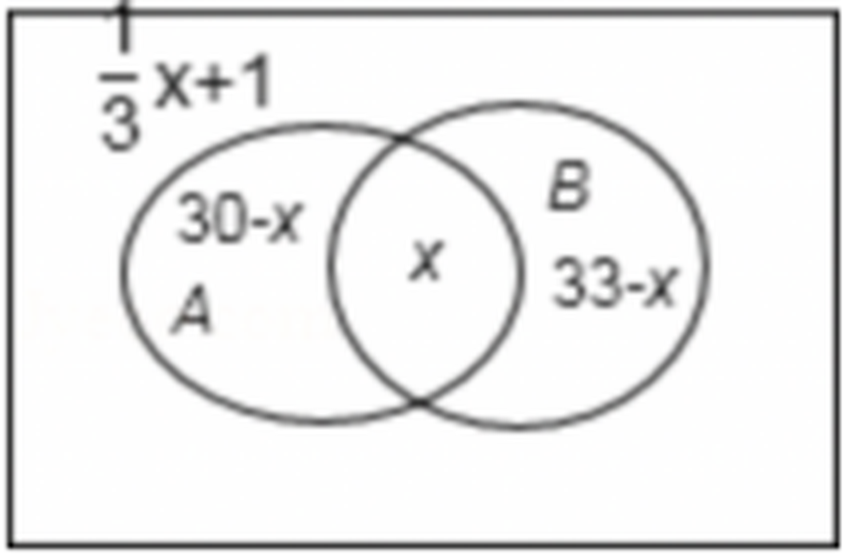
\includegraphics[width=0.30\textwidth]{figures/venn_AB_survey_50.png}
\end{center}

\ans{$21$}

\ifanswer
\solbegin
\step{由题意得赞成 $A$ 的人数 30，赞成 $B$ 的人数为 33，}
\step{设对 $A$、$B$ 都赞成的学生数为 $x$，则对 $A$、$B$ 都不赞成的学生数 $\dfrac{1}{3}x+1$，}
\step{如图得 $x+30-x+33-x+\dfrac{1}{3}x+1=50$，所以 $x=21$.}
\solend

\fi

\item 集合 $S=\{s\mid s=2n+1,n\in\Z\}$，$T=\{t\mid t=4n+1,n\in\Z\}$，则 $S$ \blankline[2.4em] $T$（填“$\subset$”“$\supset$”“$\subseteq$”或“$\supseteq$”）.

\ans{$S\supset T$}

\ifanswer
\solbegin
\step{对于 $S=\{s\mid s=2n+1,n\in\Z\}$ 为奇数，}
\step{而 $T=\{t\mid t=4n+1,n\in\Z\}$ 被 4 整除余 1 的奇数，所以 $S\supset T$.}
\solend

\fi

\item 已知集合 $A=\{x\mid -2<x<4\}$，$B=\{x\mid x^2-3ax+2a^2=0\}$，若 $A\cap B=B$，则实数 $a$ 的取值范围为 \blankline[4.4em].

\ans{$(-1,2)$}

\ifanswer
\solbegin
\step{因为 $A\cap B=B$，所以 $B\subseteq A$，}
\step{①当 $a=0$ 时，方程 $x^2-3ax+2a^2=0$ 的解为 $0$，$B\subseteq A$ 成立；}
\step{②当 $a\neq 0$ 时，方程 $x^2-3ax+2a^2=0$ 的解为 $2a$、$a$，}
\step{则 $-2<2a<4$ 且 $-2<a<4$，解得 $-1<a<2$ 且 $a\neq 0$；}
\step{综上所述，实数 $a$ 的取值范围为 $(-1,2)$.}
\solend

\fi

\item 当一个非空数集 $F$ 满足条件“若 $a$、$b\in F$，则 $a+b$、$a-b$、$ab\in F$，且当 $b\neq 0$ 时，$\dfrac{a}{b}\in F$”时，称 $F$ 为一个数域，以下四个关于数域的命题：

（1）$0$ 是任何数域的元素；（2）若数域 $F$ 有非零元素，则 $2026\in F$；

（3）集合 $P=\{x\mid x=3k,k\in\Z\}$ 为数域；（4）有理数集为数域；

其中，真命题的编号为 \blankline[4.4em]（写出所有真命题的编号）.

\ans{（1）（2）（4）}

\item 对于集合 $M$，定义函数 $f_M(x)=\begin{cases}-1,&x\in M\\ 1,&x\notin M\end{cases}$，对于两个集合 $M$、$N$，定义集合
$M\triangle N=\{x\mid f_M(x)\cdot f_N(x)=-1\}$，已知 $A=\{2,4,6,8,10\},B=\{1,2,4,8,16\}$，用 $|M|$ 表示有限集合 $M$ 中的元素个数，则对于任意集合 $M$，$|M\triangle A|+|M\triangle B|$ 的最小值为 \blankline[2.4em].

% 注：上面分段函数的第二行，原卷印作「1, $x\in M$」（两行都印 $x\in M$），与函数的定义矛盾，
%     本稿按文意订正为 $x\notin M$.
\ans{$4$}

\ifanswer
\solbegin
% 注：下面一行原卷印作「即 $M\triangle N\in\{x\mid x\in M\cup N\}$ 且 $x\in M\cap N$」，「$\in$」当为
%     「$=$」之误，且由 $f_M(x)f_N(x)=-1$ 应对应 $x\notin M\cap N$，本稿一并按文意订正.
\step{由 $M\triangle N$ 的定义得 $f_M(x)\cdot f_N(x)=-1$，}
\step{即 $M\triangle N=\{x\mid x\in M\cup N\text{ 且 }x\notin M\cap N\}$，}
\step{$|M\triangle A|+|M\triangle B|$ 要取得最小值，需满足 $A\cap B\subseteq M\subseteq A\cup B$，}
\step{此时 $|M\triangle A|+|M\triangle B|$ 的最小值为 $4$.}
\solend

\fi

\end{enumerate}

\bigsec{二、选择题}

\begin{enumerate}
\setcounter{enumi}{12}

\item 已知集合 $A=\{x\mid x=3m,m\in\N\}$，$B=\{x\mid x=3m+1,m\in\N\}$，$C=\{x\mid x=3m+2,m\in\N\}$，若 $a\in A$，$b\in B$，$c\in C$，则下列结论中可能成立的是\mbox{（\quad）}

\keepwithprev
A. $2021=a+b+c$\qquad B. $2021=abc$\qquad C. $2021=a+bc$\qquad D. $2021=a(b+c)$

\ans{C}

\ifanswer
\solbegin
\step{由题意设 $a=3m$，$b=3p+1$，$c=3n+2$，$m$、$p$、$n\in\N$，}
\step{则 $a+b+c=3m+3p+1+3n+2=3(m+p+n+1)$，}
\step{故 2021 不是 3 的整数倍，则 A 不可能；}
\step{$abc=3m(3p+1)(3n+2)$，同理 B 不可能；}
\step{$a+bc=3m+(3p+1)(3n+2)=3(m+3pn+2p+n)+2$，$2021=3\times 673+2$，}
\step{如取 $p=n=1$，则 $m=667$，即 $2021=3\times 667+4\times 5$，故 C 成立；}
\step{$a(b+c)=3m(3p+1+3n+2)=9m(p+n+1)$，同 A 可得 D 不可能.}
\step{故选 C.}
\solend

\fi

\item 设 $a$、$b$、$c$ 是实数，$x=a^2-2b+\dfrac{\pi}{3}$，$y=b^2-2c+\dfrac{\pi}{6}$，$z=c^2-2a+\dfrac{\pi}{2}$，则 $x$、$y$、$z$ 中至少有一个值\mbox{（\quad）}

\keepwithprev
A. 大于 $0$\qquad B. 等于 $0$\qquad C. 不大于 $0$\qquad D. 小于 $0$

\ans{A}

\ifanswer
\solbegin
\step{因为 $x+y+z=a^2-2b+\dfrac{\pi}{3}+b^2-2c+\dfrac{\pi}{6}+c^2-2a+\dfrac{\pi}{2}=(a-1)^2+(b-1)^2+(c-1)^2+\pi-3>0$，}
\step{假设 $x$、$y$、$z$ 都不大于 $0$，即 $x\leqslant 0$，$y\leqslant 0$，$z\leqslant 0$，}
\step{由同向不等式的可加性得 $x+y+z\leqslant 0$①，又 $x+y+z>0$ 与①式矛盾.}
\step{所以假设不成立，即原命题的结论 $x$、$y$、$z$ 中至少有一个大于 $0$. 故选 A.}
\solend

\fi

\item 命题“存在一个无理数，它的平方是有理数”的否定是\mbox{（\quad）}

\keepwithprev
A. 任意一个有理数，它的平方是有理数

B. 任意一个无理数，它的平方不是有理数

C. 存在一个有理数，它的平方是有理数

D. 存在一个无理数，它的平方不是有理数

\ans{B}

\ifanswer
\solbegin
\step{否定是任意一个无理数，它的平方不是有理数，故选 B.}
\solend

\fi

\item 设集合 $P_1=\{x\mid x^2+ax+1>0\}$，$P_2=\{x\mid x^2+ax+2>0\}$，$Q_1=\{x\mid x^2+x+b>0\}$，$Q_2=\{x\mid x^2+2x+b>0\}$，其中 $a$、$b\in\R$，下列说法正确的是\mbox{（\quad）}

\keepwithprev
A. 对任意 $a$，$P_1$ 是 $P_2$ 的子集，对任意 $b$，$Q_1$ 不是 $Q_2$ 的子集

B. 对任意 $a$，$P_1$ 是 $P_2$ 的子集，存在 $b$，使得 $Q_1$ 是 $Q_2$ 的子集

C. 对任意 $a$，使得 $P_1$ 不是 $P_2$ 的子集，对任意 $b$，$Q_1$ 不是 $Q_2$ 的子集

D. 对任意 $a$，使得 $P_1$ 不是 $P_2$ 的子集，存在 $b$，使得 $Q_1$ 不是 $Q_2$ 的子集

\ans{B}

\ifanswer
\solbegin
\step{对于集合 $P_1=\{x\mid x^2+ax+1>0\}$，$P_2=\{x\mid x^2+ax+2>0\}$，}
\step{得当 $m\in P_1$，即 $m^2+am+1>0$，得 $m^2+am+2>0$，}
\step{即有 $m\in P_2$，得对任意 $a$，$P_1$ 是 $P_2$ 的子集；}
\step{当 $b=5$ 时，$Q_1=\{x\mid x^2+x+5>0\}=\R$，$Q_2=\{x\mid x^2+2x+5>0\}=\R$，}
\step{得 $Q_1$ 是 $Q_2$ 的子集，故 A 错误，B 正确；}
\step{当 $b=1$ 时，$Q_1=\{x\mid x^2+x+1>0\}=\R$，}
\step{$Q_2=\{x\mid x^2+2x+1>0\}=\{x\mid x\neq -1\text{ 且 }x\in\R\}$，得 $Q_1$ 不是 $Q_2$ 的子集.}
\step{综上，对任意 $a$，$P_1$ 是 $P_2$ 的子集，存在 $b$，使得 $Q_1$ 是 $Q_2$ 的子集，}
\step{故 C 错误，D 错误.}
\step{故选 B.}
\solend

\fi

\end{enumerate}

\bigsec{三、解答题}

\begin{enumerate}
\setcounter{enumi}{16}

\item 已知集合 $A=\{x\mid 0<x-a\leqslant 5\}$，$B=\left\{x\mid -\dfrac{a}{2}<x\leqslant 6\right\}$.

\begin{enumerate}[label=(\arabic*)]
\item 若 $A\subseteq B$，求 $a$ 的取值范围.
\item 集合 $A$ 与 $B$ 能否相等？若能，求出 $a$ 的值，若不能，请说明理由.
\end{enumerate}

\ans{（1）$0\leqslant a\leqslant 1$；（2）不能，$a\in\varnothing$}

\ifanswer
\solbegin
\stepm{（1）}{由于 $A\subseteq B$，所以 $a+5\leqslant 6$，且 $-\dfrac{a}{2}\leqslant a$，解得 $0\leqslant a\leqslant 1$；}
\stepm{（2）}{$A=B$ 时，$a+5=6$，$-\dfrac{a}{2}=a$，解得 $a\in\varnothing$.}
\solend

\fi

\ansspace[6]

\item 已知 $\alpha:2x+m<0$，$\beta:-1<x<3$.

\begin{enumerate}[label=(\arabic*)]
\item 是否存在实数 $m$，使得 $\alpha$ 是 $\beta$ 的充分条件？若存在，求出实数 $m$ 的取值范围；
\item 是否存在实数 $m$，使得 $\alpha$ 是 $\beta$ 的必要条件？若存在，求出实数 $m$ 的取值范围.
\end{enumerate}

\ans{（1）不存在；（2）存在，$m\leqslant -6$}

\ansspace[6]

\item 已知 $\triangle ABC$ 的三边长分别为 $a,b,c$，证明：

\begin{enumerate}[label=(\arabic*)]
\item “$A=90^\circ$”是“关于 $x$ 的方程 $x^2+2ax+b^2=0$ 与 $x^2+2cx-b^2=0$ 有公共实根”的充分条件；
\item “$a=c$”是“关于 $x$ 的方程 $x^2+2ax+b^2=0$ 与 $x^2+2cx-b^2=0$ 没有公共实根”的充分非必要条件.
\end{enumerate}

\ans{（1）略；（2）略}

\ansspace[8]

\item 已知集合 $A$ 包含有 $n(n\in\N^*)$ 个元素，$A^+=\{x+y\mid x\text{、}y\in A\}$.

\begin{enumerate}[label=(\arabic*)]
\item 若 $A=\{0,1,2\}$，写出 $A^+$；
\item % 注：原卷此处印作「写出一个 $A^+$，使得 $A=A^+$」——$A$ 未给定，该问无法作答，
      %     与下方【解析】「取 $A=\{0\}$」不符，本稿按文意订正为「写出一个 $A$」.
      写出一个 $A$，使得 $A=A^+$；
\item 当 $n=4$ 时，是否存在集合 $A$，使得 $A^+=\{2,3,5,6,7,8,10\}$？若存在，求出此时的集合 $A$，若不存在，请说明理由.
\end{enumerate}

\ans{（1）$\{0,1,2,3,4\}$；（2）$A=\{0\}$；（3）不存在}

\ifanswer
\solbegin
\stepm{（1）}{由题意得 $0+0=0$，$0+1=1$，$0+2=2$，$1+1=2$，$1+2=3$，$2+2=4$ 都是 $A^+$ 中的元素，故 $A^+=\{0,1,2,3,4\}$；}
\stepm{（2）}{取 $A=\{0\}$，此时 $A^+=\{x+y\mid x\text{、}y\in A\}=\{0\}$，符合 $A=A^+$；}
\stepm{（3）}{当 $n=4$ 时，不存在集合 $A$，使得 $A^+=\{2,3,5,6,7,8,10\}$，理由如下：}
\step{假设存在 $A=\{a,b,c,d\}$，且 $a<b<c<d$，}
\step{则 $2a<a+b<a+c<b+c<b+d<c+d<2d$，}
\step{故 $2a,a+b,a+c,b+c,b+d,c+d,2d$ 为 $A^+$ 中 7 个不同的元素，}
\step{则 $2a=2$，$a+b=3$，$a+c=5$，$b+c=6$，$b+d=7$，$c+d=8$，$2d=10$，}
\step{解得 $a=1$，$b=2$，$c=4$，$d=5$，}
\step{此时 $c+d=9\in A^+$ 与 $9\notin A^+$ 矛盾，故假设不成立，}
\step{即不存在这样的集合 $A$.}
\solend

\fi

\ansspace[8]

% 压轴题：在其 \item 前先量一下版面，本页剩余高度不足 7cm 就另起一页。
\ansneed{7cm}

\item 已知集合 $A$ 为非空数集，对于集合 $A$，对 $A$ 中任意两个不同元素相加得到的和取绝对值，将这些绝对值重新组成一个新的集合，对于这一过程，我们定义为“自相加”，重新组成的集合叫做“集合 $A$ 的 1 次自相加集合”，再进行 $n-1$ 次“自相加”操作，组成的集合叫做“集合 $A$ 的 $n$ 次自相加集合”. 若集合 $A$ 的任意 $k$ 次自相加集合都不相等，则称集合 $A$ 为“完美自相加集合”，同理，我们可以定义出“$A$ 的 1 次自相减集合”，集合 $A$ 的 1 次自相加集合和 1 次自相减集合分别可表示为：$A^+=\{x\mid x=|a+b|,\ a\text{、}b\in A\}$，$A^-=\{x\mid x=|a-b|,\ a\text{、}b\in A\}$.

\begin{enumerate}[label=(\arabic*)]
\item 已知有两个集合，集合 $B=\{1,2,3,4\}$，集合 $C=\{k\mid k=2n+1,n\in\Z\}$，判断集合 $B$ 和集合 $C$ 是否是完美自相加集合，并说明理由；
\item 对（1）中的集合 $B$ 进行 11 次自相加操作后，求：集合 $B$ 的 11 次自相加集合的元素个数；
\item 若 $0\leqslant n\leqslant 2025$ 且 $n\in\N$，集合 $A=\{x\mid n\leqslant x\leqslant 2025,x\in\N\}$，$A^+\cap A^-=\varnothing$，求：$n$ 的最小值.
\end{enumerate}

\ans{（1）$B$ 是完美自相加集合，$C$ 不是完美自相加集合；（2）$2051$；（3）$675$}

\ifanswer
\solbegin
\stepm{（1）}{$B$ 是完美自相加集合，$C$ 不是完美自相加集合，}
\step{理由如下：因为集合 $B=\{1,2,3,4\}$，所以 $B^+=\{3,4,5,6,7\}$，}
\step{由此可得集合自相加后，}
\step{新的集合中最小的元素为自相加之前的集合中的最小两个元素之和，}
\step{所以显然集合 $B=\{1,2,3,4\}$ 的最小两个元素为 $1$，$2$，}
\step{所以 $B^+$ 中的最小元素为 $1+2=3$，}
\step{同理，2 次自相加后得到的集合中的最小元素是 $3+4=7$.}
\step{依照这样的规律，对集合 $B=\{1,2,3,4\}$ 进行任意次自相加操作后，}
\step{最小值总在变大，故不可能有相等集合，所以 $B$ 是完美自相加集合；}
\step{因为集合 $C=\{k\mid k=2n+1,n\in\Z\}$ 表示所有奇数构成的集合，}
\step{任何两个奇数相加的和都是偶数，}
\step{所以 $C^+=\{k\mid k=2n,n\in\Z\}$ 为所有偶数构成集合；}
\step{所以对 $C^+=\{k\mid k=2n,n\in\Z\}$ 再进行一次自相加操作，}
\step{因为任意两个偶数相加的和还是偶数，}
\step{所以后面集合不管进行多少次相加都与 $C^+=\{k\mid k=2n,n\in\Z\}$ 相同；}
\step{故 $C$ 不是完美自相加集合.}
\stepm{（2）}{由自相加性质得，对于集合 $B=\{1,2,3,4\}$，进行一次自相加，}
\step{得到集合的最小值必然是原来集合的两个最小元素值之和，}
\step{得到的最大值必然为原来集合的两个最大元素值之和，}
\step{且中间必然是连续的整数元素；}
\step{所以对集合 $B=\{1,2,3,4\}$ 进行 1 次自相加之后，}
\step{得到的集合最小两个元素为 $3$，$4$，最大的两个元素为 $6$，$7$；}
\step{进行第 2 次自相加，得到的集合最小两个元素为 $7$，$8$，}
\step{最大的两个元素为 $12$，$13$；}
\step{进行第 3 次自相加，得到的集合最小两个元素为 $15$，$16$，}
\step{最大的两个元素为 $24$，$25$；}
\step{进行第 4 次自相加，得到的集合最小两个元素为 $31$，$32$，}
\step{最大的两个元素为 $48$，$49$；}
\step{进行第 5 次自相加，得到的集合最小两个元素为 $63$，$64$，}
\step{最大的两个元素为 $96$，$97$；}
\step{进行第 6 次自相加，得到的集合最小两个元素为 $127$，$128$，}
\step{最大的两个元素为 $192$，$193$；}
\step{进行第 7 次自相加，得到的集合最小两个元素为 $255$，$256$，}
\step{最大的两个元素为 $384$，$385$；}
\step{进行第 8 次自相加，得到的集合最小两个元素为 $511$，$512$，}
\step{最大的两个元素为 $768$，$769$；}
\step{进行第 9 次自相加，得到的集合最小两个元素为 $1023$，$1024$，}
\step{最大的两个元素为 $1536$，$1537$；}
\step{进行第 10 次自相加，得到的集合最小两个元素为 $2047$，$2048$，}
\step{最大的两个元素为 $3072$，$3073$；}
\step{进行第 11 次自相加，得到的集合最小两个元素为 $4095$，$4096$，}
\step{最大的两个元素为 $6144$，$6145$；}
\step{因为集合 $B$ 的 $n$ 次自相加集合中的元素都是连续的整数，}
\step{所以集合 $B$ 进行 11 次自相加操作后的元素个数为 $6145-4095+1=2051$.}
\stepm{（3）}{因为 $0\leqslant n\leqslant 2025$ 且 $n\in\N$，集合 $A=\{x\mid n\leqslant x\leqslant 2025,x\in\N\}$，}
\step{所以 $A^+=\{x\mid 2n+1\leqslant x\leqslant 4049,x\in\N\}$，}
\step{$A^-=\{x\mid 1\leqslant x\leqslant 2025-n,x\in\N\}$，}
\step{要使 $A^+\cap A^-=\varnothing$，须使 $2n+1>2025-n$，所以 $n>\dfrac{2024}{3}=674\dfrac{2}{3}$，}
\step{又 $n\in\N$，故 $n$ 的最小值为 $675$.}
\solend

\fi

% 压轴题：其后已无内容，故作答区全用可丢弃胶水（\ansspace*）。
\ansspace*[12]

\end{enumerate}

\end{document}
"
% 紧凑版：xelatex "\def\iscompact{1}% 高一17_七宝中学_周末作业2.tex —— 高一上数学「2026-2027 年七宝中学高一上周末作业 2」（试卷版/答案版）
% 试卷版：xelatex 高一17_七宝中学_周末作业2.tex
% 答案版：xelatex "\def\isanswer{1}\input{高一17_七宝中学_周末作业2.tex}"
% 紧凑版：xelatex "\def\iscompact{1}\input{高一17_七宝中学_周末作业2.tex}"
%
% 原始材料是微信公众号图文（公众号「魔都数学加油站」），正文为 10 张 PNG 页（1080×1527）。
% 原文本身就是一份**讲评版**——题目下方直接印出【答案】或【解析】，选择题的答案印在解析末句
% 「故选 X」里。试题文字、答案与解析均照原卷录入（订正处见下），卷面上的粉色斜水印
% 「魔都数学加油站」属水印，未录入。
%
% 与原卷的排版差异（均已在 README「说明」中交代）：
%   ① 原文自**第 3 题**起（第 1、2 题未在该文中发布），故本稿题号亦自 3 起；
%   ② 原卷本就印有「一、填空题」「二、选择题」「三、解答题」三节标题（分别在原图 00/02/04.png
%      上，逐页核对过），本稿照原卷分节，只把标题改排成全稿统一的「大节标题」样式；
%   ③ 原卷填空、选择的答案直接印在题目下方（选择题只在解析末句「故选 X」中给出），本稿统一改为
%      试卷版隐去、答案版以【答案】给出，选择题的括注一律改排「\mbox{（\quad）}」并把答案移到选项之后，
%      使两版彻底分离；
%   ④ 原卷的集合符号大小写混用：第 3 题题干的实数集印成**粗体** $\mathbf{R}$，第 16 题题干与
%      第 16 题解析的印成正体 $R$；自然数集 $N$、整数集 $Z$ 一律正体。本稿按全稿惯例统一写作
%      $\R$、$\N$、$\Z$；
%   ⑤ 原卷未印副标题，本稿按全稿惯例补出副标题「集合与常用逻辑用语」；
%   ⑥ 原卷解答题子问编号为「（1）（2）」，本稿用嵌套 enumerate 排成同一形态；原卷第 15 题的
%      D 选项因原页翻页被截到下一页首页，本稿自然连排；
%   ⑦ 原卷解答题未留作答空间（讲评稿通篇是答案），本稿逐题补出书写留白，仅试卷版显示；
%   ⑧ 第 21 题题干里 $A^+$、$A^-$ 的定义含绝对值号（原卷作 $\{x\mid x=|a+b|,\ a\text{、}b\in A\}$
%      与 $\{x\mid x=|a-b|,\ a\text{、}b\in A\}$），本稿照原卷录入；2026-09-15 回原图逐处放大复核
%      时发现曾漏抄两处绝对值号、并把分隔逗号误写成 $\mid$，已按原卷订正（见 README 专记）。
%
% 原卷笔误三处（均已放大到能看清字形后核对，本稿按文意订正，并在 README 中写明原委）：
%   ① 第 12 题题干的分段函数 $f_M(x)$ 原卷两行都印作「$x\in M$」（$-1$ 与 $1$ 都取在 $M$ 上），
%      与「函数」的定义直接矛盾（$M$ 上无法同时取两个值），按文意订正第二行为 $x\notin M$；
%   ② 第 12 题【解析】首行原卷印「即 $M\triangle N\in\{x\mid x\in M\cup N\}$ 且 $x\in M\cap N$」，
%      其中「$\in$」当为「$=$」之误；且由 $f_M(x)f_N(x)=-1$ 应对应 $x\notin M\cap N$（原卷印作
%      $x\in M\cap N$，与上一行刚写出的对称差的定义相矛盾），本稿一并订正；
%   ③ 第 20 题(2)原卷印「写出一个 $A^+$，使得 $A=A^+$」——$A$ 未给定，该问无法作答，与紧接的
%      【解析】「取 $A=\{0\}$，此时 $A^+=\{0\}$，符合 $A=A^+$」不符，本稿按文意订正为
%      「写出一个 $A$，使得 $A=A^+$」.
%
% 原卷存疑一处（无法确证原意，本稿照抄原卷、未改）：
%   ① 第 5 题 ④ 原卷题干印 $S=\{x\mid |x|\leqslant\sqrt{3},x\in N\}$（该字母与 ③ 中的 $Z$
%      字形明显不同，$Z$ 有上下两横，已放大比对确认），而【解析】印「因为 $S=\{-1,0,1\}$」——
%      按 $x\in N$ 应为 $S=\{0,1\}$（或 $\{1\}$），题干与解析的口径不一致；但无论取哪一口径，
%      ④ 都是 $M$ 的子集、本题结论（填④）不变，故题干与解析均照抄原卷，未改。

\documentclass[a4paper,11pt]{article}
\usepackage{common}

\begin{document}

\examtitlest{2026--2027 年七宝中学高一上周末作业 2}{集合与常用逻辑用语}

\bigsec{一、填空题}

\begin{enumerate}
\setcounter{enumi}{2}

\item 已知 $a,x\in\R$，则“$x\in\{-a,a\}$”是“$|x|=a$”的 \blankline[4.4em] 条件.

\ans{必要不充分}

\item 设全集为 $U$，$A\subseteq U$，$B\subseteq U$，则“$A\subset B$”是“$\overline{B}\subset\overline{A}$”的 \blankline[4.4em] 条件.

\ans{充要}

\item 已知集合 $M=\{x\mid -\sqrt{5}<x<\sqrt{3},x\in\Z\}$，则下列集合是集合 $M$ 的子集的是 \blankline[4.4em]（填序号）.

① $P=\{-3,0,1\}$；② $Q=\{-1,0,1,2\}$；③ $R=\{y\mid -\pi<y<-1,y\in\Z\}$；

④ $S=\{x\mid |x|\leqslant\sqrt{3},x\in\N\}$.

\ans{④}

\ifanswer
\solbegin
\step{由已知得集合 $M=\{-2,-1,0,1\}$，}
\step{所以由子集的定义得选项①错误，②错误，}
\step{因为 $R=\{-3,-2\}$，所以集合 $R$ 不表示集合 $M$ 的子集，③错误，}
\step{因为 $S=\{-1,0,1\}$，所以是集合 $M$ 的子集，故正确.}
\step{故是集合 $M$ 的子集的是④.}
\solend

\fi

\item 已知 $x\in\R$，用反证法证明命题“若 $x^2-7x+10<0$，则 $2<x<5$”时，应该假设 \blankline[5em].

\ans{$x\leqslant 2$ 或 $x\geqslant 5$}

\item 设 $a_1,b_1,c_1,a_2,b_2,c_2$ 均为非零实数，方程 $a_1x^2+b_1x+c_1=0$ 和 $a_2x^2+b_2x+c_2=0$ 的解集分别为 $M$ 和 $N$，那么“$\dfrac{a_1}{a_2}=\dfrac{b_1}{b_2}=\dfrac{c_1}{c_2}$”是“$M=N$”的 \blankline[4.4em] 条件.

（填“充分非必要”、“必要非充分”、“充要”、或“既非充分又非必要”）

\ans{充分非必要}

\ifanswer
\solbegin
\step{$\dfrac{a_1}{a_2}=\dfrac{b_1}{b_2}=\dfrac{c_1}{c_2}$ 能推出 $M=N$，}
\step{若 $M=N=\varnothing$ 推不出 $\dfrac{a_1}{a_2}=\dfrac{b_1}{b_2}=\dfrac{c_1}{c_2}$，}
\step{所以“$\dfrac{a_1}{a_2}=\dfrac{b_1}{b_2}=\dfrac{c_1}{c_2}$”是“$M=N$”的“充分非必要”条件.}
\solend

\fi

\item 向 50 名学生调查对 $A$、$B$ 两事件的态度，有如下结果赞成 $A$ 的人数是全体的五分之三，其余的不赞成，赞成 $B$ 的比赞成 $A$ 的多 3 人，其余的不赞成；另外，对 $A$、$B$ 都不赞成的学生数比对 $A$、$B$ 都赞成的学生数的三分之一多 1 人. 则对 $A$、$B$ 都赞成的学生有 \blankline[2.4em] 人.

\begin{center}
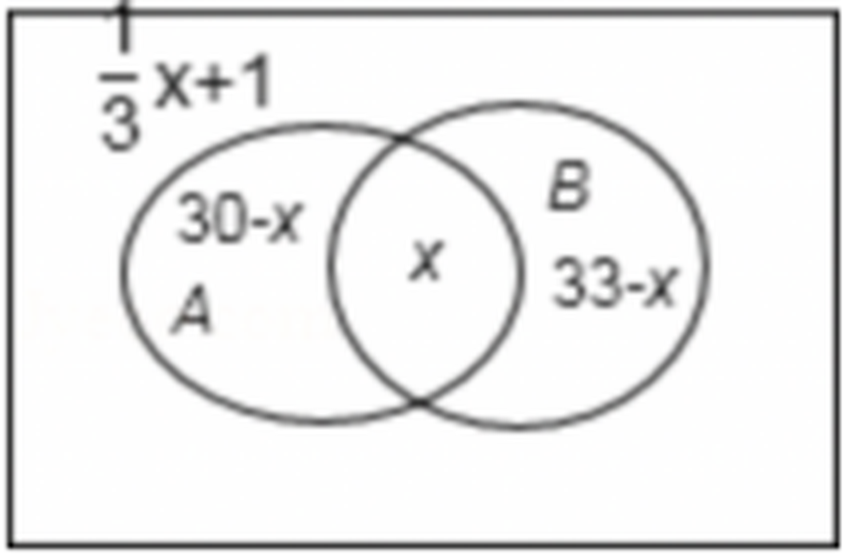
\includegraphics[width=0.30\textwidth]{figures/venn_AB_survey_50.png}
\end{center}

\ans{$21$}

\ifanswer
\solbegin
\step{由题意得赞成 $A$ 的人数 30，赞成 $B$ 的人数为 33，}
\step{设对 $A$、$B$ 都赞成的学生数为 $x$，则对 $A$、$B$ 都不赞成的学生数 $\dfrac{1}{3}x+1$，}
\step{如图得 $x+30-x+33-x+\dfrac{1}{3}x+1=50$，所以 $x=21$.}
\solend

\fi

\item 集合 $S=\{s\mid s=2n+1,n\in\Z\}$，$T=\{t\mid t=4n+1,n\in\Z\}$，则 $S$ \blankline[2.4em] $T$（填“$\subset$”“$\supset$”“$\subseteq$”或“$\supseteq$”）.

\ans{$S\supset T$}

\ifanswer
\solbegin
\step{对于 $S=\{s\mid s=2n+1,n\in\Z\}$ 为奇数，}
\step{而 $T=\{t\mid t=4n+1,n\in\Z\}$ 被 4 整除余 1 的奇数，所以 $S\supset T$.}
\solend

\fi

\item 已知集合 $A=\{x\mid -2<x<4\}$，$B=\{x\mid x^2-3ax+2a^2=0\}$，若 $A\cap B=B$，则实数 $a$ 的取值范围为 \blankline[4.4em].

\ans{$(-1,2)$}

\ifanswer
\solbegin
\step{因为 $A\cap B=B$，所以 $B\subseteq A$，}
\step{①当 $a=0$ 时，方程 $x^2-3ax+2a^2=0$ 的解为 $0$，$B\subseteq A$ 成立；}
\step{②当 $a\neq 0$ 时，方程 $x^2-3ax+2a^2=0$ 的解为 $2a$、$a$，}
\step{则 $-2<2a<4$ 且 $-2<a<4$，解得 $-1<a<2$ 且 $a\neq 0$；}
\step{综上所述，实数 $a$ 的取值范围为 $(-1,2)$.}
\solend

\fi

\item 当一个非空数集 $F$ 满足条件“若 $a$、$b\in F$，则 $a+b$、$a-b$、$ab\in F$，且当 $b\neq 0$ 时，$\dfrac{a}{b}\in F$”时，称 $F$ 为一个数域，以下四个关于数域的命题：

（1）$0$ 是任何数域的元素；（2）若数域 $F$ 有非零元素，则 $2026\in F$；

（3）集合 $P=\{x\mid x=3k,k\in\Z\}$ 为数域；（4）有理数集为数域；

其中，真命题的编号为 \blankline[4.4em]（写出所有真命题的编号）.

\ans{（1）（2）（4）}

\item 对于集合 $M$，定义函数 $f_M(x)=\begin{cases}-1,&x\in M\\ 1,&x\notin M\end{cases}$，对于两个集合 $M$、$N$，定义集合
$M\triangle N=\{x\mid f_M(x)\cdot f_N(x)=-1\}$，已知 $A=\{2,4,6,8,10\},B=\{1,2,4,8,16\}$，用 $|M|$ 表示有限集合 $M$ 中的元素个数，则对于任意集合 $M$，$|M\triangle A|+|M\triangle B|$ 的最小值为 \blankline[2.4em].

% 注：上面分段函数的第二行，原卷印作「1, $x\in M$」（两行都印 $x\in M$），与函数的定义矛盾，
%     本稿按文意订正为 $x\notin M$.
\ans{$4$}

\ifanswer
\solbegin
% 注：下面一行原卷印作「即 $M\triangle N\in\{x\mid x\in M\cup N\}$ 且 $x\in M\cap N$」，「$\in$」当为
%     「$=$」之误，且由 $f_M(x)f_N(x)=-1$ 应对应 $x\notin M\cap N$，本稿一并按文意订正.
\step{由 $M\triangle N$ 的定义得 $f_M(x)\cdot f_N(x)=-1$，}
\step{即 $M\triangle N=\{x\mid x\in M\cup N\text{ 且 }x\notin M\cap N\}$，}
\step{$|M\triangle A|+|M\triangle B|$ 要取得最小值，需满足 $A\cap B\subseteq M\subseteq A\cup B$，}
\step{此时 $|M\triangle A|+|M\triangle B|$ 的最小值为 $4$.}
\solend

\fi

\end{enumerate}

\bigsec{二、选择题}

\begin{enumerate}
\setcounter{enumi}{12}

\item 已知集合 $A=\{x\mid x=3m,m\in\N\}$，$B=\{x\mid x=3m+1,m\in\N\}$，$C=\{x\mid x=3m+2,m\in\N\}$，若 $a\in A$，$b\in B$，$c\in C$，则下列结论中可能成立的是\mbox{（\quad）}

\keepwithprev
A. $2021=a+b+c$\qquad B. $2021=abc$\qquad C. $2021=a+bc$\qquad D. $2021=a(b+c)$

\ans{C}

\ifanswer
\solbegin
\step{由题意设 $a=3m$，$b=3p+1$，$c=3n+2$，$m$、$p$、$n\in\N$，}
\step{则 $a+b+c=3m+3p+1+3n+2=3(m+p+n+1)$，}
\step{故 2021 不是 3 的整数倍，则 A 不可能；}
\step{$abc=3m(3p+1)(3n+2)$，同理 B 不可能；}
\step{$a+bc=3m+(3p+1)(3n+2)=3(m+3pn+2p+n)+2$，$2021=3\times 673+2$，}
\step{如取 $p=n=1$，则 $m=667$，即 $2021=3\times 667+4\times 5$，故 C 成立；}
\step{$a(b+c)=3m(3p+1+3n+2)=9m(p+n+1)$，同 A 可得 D 不可能.}
\step{故选 C.}
\solend

\fi

\item 设 $a$、$b$、$c$ 是实数，$x=a^2-2b+\dfrac{\pi}{3}$，$y=b^2-2c+\dfrac{\pi}{6}$，$z=c^2-2a+\dfrac{\pi}{2}$，则 $x$、$y$、$z$ 中至少有一个值\mbox{（\quad）}

\keepwithprev
A. 大于 $0$\qquad B. 等于 $0$\qquad C. 不大于 $0$\qquad D. 小于 $0$

\ans{A}

\ifanswer
\solbegin
\step{因为 $x+y+z=a^2-2b+\dfrac{\pi}{3}+b^2-2c+\dfrac{\pi}{6}+c^2-2a+\dfrac{\pi}{2}=(a-1)^2+(b-1)^2+(c-1)^2+\pi-3>0$，}
\step{假设 $x$、$y$、$z$ 都不大于 $0$，即 $x\leqslant 0$，$y\leqslant 0$，$z\leqslant 0$，}
\step{由同向不等式的可加性得 $x+y+z\leqslant 0$①，又 $x+y+z>0$ 与①式矛盾.}
\step{所以假设不成立，即原命题的结论 $x$、$y$、$z$ 中至少有一个大于 $0$. 故选 A.}
\solend

\fi

\item 命题“存在一个无理数，它的平方是有理数”的否定是\mbox{（\quad）}

\keepwithprev
A. 任意一个有理数，它的平方是有理数

B. 任意一个无理数，它的平方不是有理数

C. 存在一个有理数，它的平方是有理数

D. 存在一个无理数，它的平方不是有理数

\ans{B}

\ifanswer
\solbegin
\step{否定是任意一个无理数，它的平方不是有理数，故选 B.}
\solend

\fi

\item 设集合 $P_1=\{x\mid x^2+ax+1>0\}$，$P_2=\{x\mid x^2+ax+2>0\}$，$Q_1=\{x\mid x^2+x+b>0\}$，$Q_2=\{x\mid x^2+2x+b>0\}$，其中 $a$、$b\in\R$，下列说法正确的是\mbox{（\quad）}

\keepwithprev
A. 对任意 $a$，$P_1$ 是 $P_2$ 的子集，对任意 $b$，$Q_1$ 不是 $Q_2$ 的子集

B. 对任意 $a$，$P_1$ 是 $P_2$ 的子集，存在 $b$，使得 $Q_1$ 是 $Q_2$ 的子集

C. 对任意 $a$，使得 $P_1$ 不是 $P_2$ 的子集，对任意 $b$，$Q_1$ 不是 $Q_2$ 的子集

D. 对任意 $a$，使得 $P_1$ 不是 $P_2$ 的子集，存在 $b$，使得 $Q_1$ 不是 $Q_2$ 的子集

\ans{B}

\ifanswer
\solbegin
\step{对于集合 $P_1=\{x\mid x^2+ax+1>0\}$，$P_2=\{x\mid x^2+ax+2>0\}$，}
\step{得当 $m\in P_1$，即 $m^2+am+1>0$，得 $m^2+am+2>0$，}
\step{即有 $m\in P_2$，得对任意 $a$，$P_1$ 是 $P_2$ 的子集；}
\step{当 $b=5$ 时，$Q_1=\{x\mid x^2+x+5>0\}=\R$，$Q_2=\{x\mid x^2+2x+5>0\}=\R$，}
\step{得 $Q_1$ 是 $Q_2$ 的子集，故 A 错误，B 正确；}
\step{当 $b=1$ 时，$Q_1=\{x\mid x^2+x+1>0\}=\R$，}
\step{$Q_2=\{x\mid x^2+2x+1>0\}=\{x\mid x\neq -1\text{ 且 }x\in\R\}$，得 $Q_1$ 不是 $Q_2$ 的子集.}
\step{综上，对任意 $a$，$P_1$ 是 $P_2$ 的子集，存在 $b$，使得 $Q_1$ 是 $Q_2$ 的子集，}
\step{故 C 错误，D 错误.}
\step{故选 B.}
\solend

\fi

\end{enumerate}

\bigsec{三、解答题}

\begin{enumerate}
\setcounter{enumi}{16}

\item 已知集合 $A=\{x\mid 0<x-a\leqslant 5\}$，$B=\left\{x\mid -\dfrac{a}{2}<x\leqslant 6\right\}$.

\begin{enumerate}[label=(\arabic*)]
\item 若 $A\subseteq B$，求 $a$ 的取值范围.
\item 集合 $A$ 与 $B$ 能否相等？若能，求出 $a$ 的值，若不能，请说明理由.
\end{enumerate}

\ans{（1）$0\leqslant a\leqslant 1$；（2）不能，$a\in\varnothing$}

\ifanswer
\solbegin
\stepm{（1）}{由于 $A\subseteq B$，所以 $a+5\leqslant 6$，且 $-\dfrac{a}{2}\leqslant a$，解得 $0\leqslant a\leqslant 1$；}
\stepm{（2）}{$A=B$ 时，$a+5=6$，$-\dfrac{a}{2}=a$，解得 $a\in\varnothing$.}
\solend

\fi

\ansspace[6]

\item 已知 $\alpha:2x+m<0$，$\beta:-1<x<3$.

\begin{enumerate}[label=(\arabic*)]
\item 是否存在实数 $m$，使得 $\alpha$ 是 $\beta$ 的充分条件？若存在，求出实数 $m$ 的取值范围；
\item 是否存在实数 $m$，使得 $\alpha$ 是 $\beta$ 的必要条件？若存在，求出实数 $m$ 的取值范围.
\end{enumerate}

\ans{（1）不存在；（2）存在，$m\leqslant -6$}

\ansspace[6]

\item 已知 $\triangle ABC$ 的三边长分别为 $a,b,c$，证明：

\begin{enumerate}[label=(\arabic*)]
\item “$A=90^\circ$”是“关于 $x$ 的方程 $x^2+2ax+b^2=0$ 与 $x^2+2cx-b^2=0$ 有公共实根”的充分条件；
\item “$a=c$”是“关于 $x$ 的方程 $x^2+2ax+b^2=0$ 与 $x^2+2cx-b^2=0$ 没有公共实根”的充分非必要条件.
\end{enumerate}

\ans{（1）略；（2）略}

\ansspace[8]

\item 已知集合 $A$ 包含有 $n(n\in\N^*)$ 个元素，$A^+=\{x+y\mid x\text{、}y\in A\}$.

\begin{enumerate}[label=(\arabic*)]
\item 若 $A=\{0,1,2\}$，写出 $A^+$；
\item % 注：原卷此处印作「写出一个 $A^+$，使得 $A=A^+$」——$A$ 未给定，该问无法作答，
      %     与下方【解析】「取 $A=\{0\}$」不符，本稿按文意订正为「写出一个 $A$」.
      写出一个 $A$，使得 $A=A^+$；
\item 当 $n=4$ 时，是否存在集合 $A$，使得 $A^+=\{2,3,5,6,7,8,10\}$？若存在，求出此时的集合 $A$，若不存在，请说明理由.
\end{enumerate}

\ans{（1）$\{0,1,2,3,4\}$；（2）$A=\{0\}$；（3）不存在}

\ifanswer
\solbegin
\stepm{（1）}{由题意得 $0+0=0$，$0+1=1$，$0+2=2$，$1+1=2$，$1+2=3$，$2+2=4$ 都是 $A^+$ 中的元素，故 $A^+=\{0,1,2,3,4\}$；}
\stepm{（2）}{取 $A=\{0\}$，此时 $A^+=\{x+y\mid x\text{、}y\in A\}=\{0\}$，符合 $A=A^+$；}
\stepm{（3）}{当 $n=4$ 时，不存在集合 $A$，使得 $A^+=\{2,3,5,6,7,8,10\}$，理由如下：}
\step{假设存在 $A=\{a,b,c,d\}$，且 $a<b<c<d$，}
\step{则 $2a<a+b<a+c<b+c<b+d<c+d<2d$，}
\step{故 $2a,a+b,a+c,b+c,b+d,c+d,2d$ 为 $A^+$ 中 7 个不同的元素，}
\step{则 $2a=2$，$a+b=3$，$a+c=5$，$b+c=6$，$b+d=7$，$c+d=8$，$2d=10$，}
\step{解得 $a=1$，$b=2$，$c=4$，$d=5$，}
\step{此时 $c+d=9\in A^+$ 与 $9\notin A^+$ 矛盾，故假设不成立，}
\step{即不存在这样的集合 $A$.}
\solend

\fi

\ansspace[8]

% 压轴题：在其 \item 前先量一下版面，本页剩余高度不足 7cm 就另起一页。
\ansneed{7cm}

\item 已知集合 $A$ 为非空数集，对于集合 $A$，对 $A$ 中任意两个不同元素相加得到的和取绝对值，将这些绝对值重新组成一个新的集合，对于这一过程，我们定义为“自相加”，重新组成的集合叫做“集合 $A$ 的 1 次自相加集合”，再进行 $n-1$ 次“自相加”操作，组成的集合叫做“集合 $A$ 的 $n$ 次自相加集合”. 若集合 $A$ 的任意 $k$ 次自相加集合都不相等，则称集合 $A$ 为“完美自相加集合”，同理，我们可以定义出“$A$ 的 1 次自相减集合”，集合 $A$ 的 1 次自相加集合和 1 次自相减集合分别可表示为：$A^+=\{x\mid x=|a+b|,\ a\text{、}b\in A\}$，$A^-=\{x\mid x=|a-b|,\ a\text{、}b\in A\}$.

\begin{enumerate}[label=(\arabic*)]
\item 已知有两个集合，集合 $B=\{1,2,3,4\}$，集合 $C=\{k\mid k=2n+1,n\in\Z\}$，判断集合 $B$ 和集合 $C$ 是否是完美自相加集合，并说明理由；
\item 对（1）中的集合 $B$ 进行 11 次自相加操作后，求：集合 $B$ 的 11 次自相加集合的元素个数；
\item 若 $0\leqslant n\leqslant 2025$ 且 $n\in\N$，集合 $A=\{x\mid n\leqslant x\leqslant 2025,x\in\N\}$，$A^+\cap A^-=\varnothing$，求：$n$ 的最小值.
\end{enumerate}

\ans{（1）$B$ 是完美自相加集合，$C$ 不是完美自相加集合；（2）$2051$；（3）$675$}

\ifanswer
\solbegin
\stepm{（1）}{$B$ 是完美自相加集合，$C$ 不是完美自相加集合，}
\step{理由如下：因为集合 $B=\{1,2,3,4\}$，所以 $B^+=\{3,4,5,6,7\}$，}
\step{由此可得集合自相加后，}
\step{新的集合中最小的元素为自相加之前的集合中的最小两个元素之和，}
\step{所以显然集合 $B=\{1,2,3,4\}$ 的最小两个元素为 $1$，$2$，}
\step{所以 $B^+$ 中的最小元素为 $1+2=3$，}
\step{同理，2 次自相加后得到的集合中的最小元素是 $3+4=7$.}
\step{依照这样的规律，对集合 $B=\{1,2,3,4\}$ 进行任意次自相加操作后，}
\step{最小值总在变大，故不可能有相等集合，所以 $B$ 是完美自相加集合；}
\step{因为集合 $C=\{k\mid k=2n+1,n\in\Z\}$ 表示所有奇数构成的集合，}
\step{任何两个奇数相加的和都是偶数，}
\step{所以 $C^+=\{k\mid k=2n,n\in\Z\}$ 为所有偶数构成集合；}
\step{所以对 $C^+=\{k\mid k=2n,n\in\Z\}$ 再进行一次自相加操作，}
\step{因为任意两个偶数相加的和还是偶数，}
\step{所以后面集合不管进行多少次相加都与 $C^+=\{k\mid k=2n,n\in\Z\}$ 相同；}
\step{故 $C$ 不是完美自相加集合.}
\stepm{（2）}{由自相加性质得，对于集合 $B=\{1,2,3,4\}$，进行一次自相加，}
\step{得到集合的最小值必然是原来集合的两个最小元素值之和，}
\step{得到的最大值必然为原来集合的两个最大元素值之和，}
\step{且中间必然是连续的整数元素；}
\step{所以对集合 $B=\{1,2,3,4\}$ 进行 1 次自相加之后，}
\step{得到的集合最小两个元素为 $3$，$4$，最大的两个元素为 $6$，$7$；}
\step{进行第 2 次自相加，得到的集合最小两个元素为 $7$，$8$，}
\step{最大的两个元素为 $12$，$13$；}
\step{进行第 3 次自相加，得到的集合最小两个元素为 $15$，$16$，}
\step{最大的两个元素为 $24$，$25$；}
\step{进行第 4 次自相加，得到的集合最小两个元素为 $31$，$32$，}
\step{最大的两个元素为 $48$，$49$；}
\step{进行第 5 次自相加，得到的集合最小两个元素为 $63$，$64$，}
\step{最大的两个元素为 $96$，$97$；}
\step{进行第 6 次自相加，得到的集合最小两个元素为 $127$，$128$，}
\step{最大的两个元素为 $192$，$193$；}
\step{进行第 7 次自相加，得到的集合最小两个元素为 $255$，$256$，}
\step{最大的两个元素为 $384$，$385$；}
\step{进行第 8 次自相加，得到的集合最小两个元素为 $511$，$512$，}
\step{最大的两个元素为 $768$，$769$；}
\step{进行第 9 次自相加，得到的集合最小两个元素为 $1023$，$1024$，}
\step{最大的两个元素为 $1536$，$1537$；}
\step{进行第 10 次自相加，得到的集合最小两个元素为 $2047$，$2048$，}
\step{最大的两个元素为 $3072$，$3073$；}
\step{进行第 11 次自相加，得到的集合最小两个元素为 $4095$，$4096$，}
\step{最大的两个元素为 $6144$，$6145$；}
\step{因为集合 $B$ 的 $n$ 次自相加集合中的元素都是连续的整数，}
\step{所以集合 $B$ 进行 11 次自相加操作后的元素个数为 $6145-4095+1=2051$.}
\stepm{（3）}{因为 $0\leqslant n\leqslant 2025$ 且 $n\in\N$，集合 $A=\{x\mid n\leqslant x\leqslant 2025,x\in\N\}$，}
\step{所以 $A^+=\{x\mid 2n+1\leqslant x\leqslant 4049,x\in\N\}$，}
\step{$A^-=\{x\mid 1\leqslant x\leqslant 2025-n,x\in\N\}$，}
\step{要使 $A^+\cap A^-=\varnothing$，须使 $2n+1>2025-n$，所以 $n>\dfrac{2024}{3}=674\dfrac{2}{3}$，}
\step{又 $n\in\N$，故 $n$ 的最小值为 $675$.}
\solend

\fi

% 压轴题：其后已无内容，故作答区全用可丢弃胶水（\ansspace*）。
\ansspace*[12]

\end{enumerate}

\end{document}
"
%
% 原始材料是微信公众号图文（公众号「魔都数学加油站」），正文为 10 张 PNG 页（1080×1527）。
% 原文本身就是一份**讲评版**——题目下方直接印出【答案】或【解析】，选择题的答案印在解析末句
% 「故选 X」里。试题文字、答案与解析均照原卷录入（订正处见下），卷面上的粉色斜水印
% 「魔都数学加油站」属水印，未录入。
%
% 与原卷的排版差异（均已在 README「说明」中交代）：
%   ① 原文自**第 3 题**起（第 1、2 题未在该文中发布），故本稿题号亦自 3 起；
%   ② 原卷本就印有「一、填空题」「二、选择题」「三、解答题」三节标题（分别在原图 00/02/04.png
%      上，逐页核对过），本稿照原卷分节，只把标题改排成全稿统一的「大节标题」样式；
%   ③ 原卷填空、选择的答案直接印在题目下方（选择题只在解析末句「故选 X」中给出），本稿统一改为
%      试卷版隐去、答案版以【答案】给出，选择题的括注一律改排「\mbox{（\quad）}」并把答案移到选项之后，
%      使两版彻底分离；
%   ④ 原卷的集合符号大小写混用：第 3 题题干的实数集印成**粗体** $\mathbf{R}$，第 16 题题干与
%      第 16 题解析的印成正体 $R$；自然数集 $N$、整数集 $Z$ 一律正体。本稿按全稿惯例统一写作
%      $\R$、$\N$、$\Z$；
%   ⑤ 原卷未印副标题，本稿按全稿惯例补出副标题「集合与常用逻辑用语」；
%   ⑥ 原卷解答题子问编号为「（1）（2）」，本稿用嵌套 enumerate 排成同一形态；原卷第 15 题的
%      D 选项因原页翻页被截到下一页首页，本稿自然连排；
%   ⑦ 原卷解答题未留作答空间（讲评稿通篇是答案），本稿逐题补出书写留白，仅试卷版显示；
%   ⑧ 第 21 题题干里 $A^+$、$A^-$ 的定义含绝对值号（原卷作 $\{x\mid x=|a+b|,\ a\text{、}b\in A\}$
%      与 $\{x\mid x=|a-b|,\ a\text{、}b\in A\}$），本稿照原卷录入；2026-09-15 回原图逐处放大复核
%      时发现曾漏抄两处绝对值号、并把分隔逗号误写成 $\mid$，已按原卷订正（见 README 专记）。
%
% 原卷笔误三处（均已放大到能看清字形后核对，本稿按文意订正，并在 README 中写明原委）：
%   ① 第 12 题题干的分段函数 $f_M(x)$ 原卷两行都印作「$x\in M$」（$-1$ 与 $1$ 都取在 $M$ 上），
%      与「函数」的定义直接矛盾（$M$ 上无法同时取两个值），按文意订正第二行为 $x\notin M$；
%   ② 第 12 题【解析】首行原卷印「即 $M\triangle N\in\{x\mid x\in M\cup N\}$ 且 $x\in M\cap N$」，
%      其中「$\in$」当为「$=$」之误；且由 $f_M(x)f_N(x)=-1$ 应对应 $x\notin M\cap N$（原卷印作
%      $x\in M\cap N$，与上一行刚写出的对称差的定义相矛盾），本稿一并订正；
%   ③ 第 20 题(2)原卷印「写出一个 $A^+$，使得 $A=A^+$」——$A$ 未给定，该问无法作答，与紧接的
%      【解析】「取 $A=\{0\}$，此时 $A^+=\{0\}$，符合 $A=A^+$」不符，本稿按文意订正为
%      「写出一个 $A$，使得 $A=A^+$」.
%
% 原卷存疑一处（无法确证原意，本稿照抄原卷、未改）：
%   ① 第 5 题 ④ 原卷题干印 $S=\{x\mid |x|\leqslant\sqrt{3},x\in N\}$（该字母与 ③ 中的 $Z$
%      字形明显不同，$Z$ 有上下两横，已放大比对确认），而【解析】印「因为 $S=\{-1,0,1\}$」——
%      按 $x\in N$ 应为 $S=\{0,1\}$（或 $\{1\}$），题干与解析的口径不一致；但无论取哪一口径，
%      ④ 都是 $M$ 的子集、本题结论（填④）不变，故题干与解析均照抄原卷，未改。

\documentclass[a4paper,11pt]{article}
\usepackage{common}

\begin{document}

\examtitlest{2026--2027 年七宝中学高一上周末作业 2}{集合与常用逻辑用语}

\bigsec{一、填空题}

\begin{enumerate}
\setcounter{enumi}{2}

\item 已知 $a,x\in\R$，则“$x\in\{-a,a\}$”是“$|x|=a$”的 \blankline[4.4em] 条件.

\ans{必要不充分}

\item 设全集为 $U$，$A\subseteq U$，$B\subseteq U$，则“$A\subset B$”是“$\overline{B}\subset\overline{A}$”的 \blankline[4.4em] 条件.

\ans{充要}

\item 已知集合 $M=\{x\mid -\sqrt{5}<x<\sqrt{3},x\in\Z\}$，则下列集合是集合 $M$ 的子集的是 \blankline[4.4em]（填序号）.

① $P=\{-3,0,1\}$；② $Q=\{-1,0,1,2\}$；③ $R=\{y\mid -\pi<y<-1,y\in\Z\}$；

④ $S=\{x\mid |x|\leqslant\sqrt{3},x\in\N\}$.

\ans{④}

\ifanswer
\solbegin
\step{由已知得集合 $M=\{-2,-1,0,1\}$，}
\step{所以由子集的定义得选项①错误，②错误，}
\step{因为 $R=\{-3,-2\}$，所以集合 $R$ 不表示集合 $M$ 的子集，③错误，}
\step{因为 $S=\{-1,0,1\}$，所以是集合 $M$ 的子集，故正确.}
\step{故是集合 $M$ 的子集的是④.}
\solend

\fi

\item 已知 $x\in\R$，用反证法证明命题“若 $x^2-7x+10<0$，则 $2<x<5$”时，应该假设 \blankline[5em].

\ans{$x\leqslant 2$ 或 $x\geqslant 5$}

\item 设 $a_1,b_1,c_1,a_2,b_2,c_2$ 均为非零实数，方程 $a_1x^2+b_1x+c_1=0$ 和 $a_2x^2+b_2x+c_2=0$ 的解集分别为 $M$ 和 $N$，那么“$\dfrac{a_1}{a_2}=\dfrac{b_1}{b_2}=\dfrac{c_1}{c_2}$”是“$M=N$”的 \blankline[4.4em] 条件.

（填“充分非必要”、“必要非充分”、“充要”、或“既非充分又非必要”）

\ans{充分非必要}

\ifanswer
\solbegin
\step{$\dfrac{a_1}{a_2}=\dfrac{b_1}{b_2}=\dfrac{c_1}{c_2}$ 能推出 $M=N$，}
\step{若 $M=N=\varnothing$ 推不出 $\dfrac{a_1}{a_2}=\dfrac{b_1}{b_2}=\dfrac{c_1}{c_2}$，}
\step{所以“$\dfrac{a_1}{a_2}=\dfrac{b_1}{b_2}=\dfrac{c_1}{c_2}$”是“$M=N$”的“充分非必要”条件.}
\solend

\fi

\item 向 50 名学生调查对 $A$、$B$ 两事件的态度，有如下结果赞成 $A$ 的人数是全体的五分之三，其余的不赞成，赞成 $B$ 的比赞成 $A$ 的多 3 人，其余的不赞成；另外，对 $A$、$B$ 都不赞成的学生数比对 $A$、$B$ 都赞成的学生数的三分之一多 1 人. 则对 $A$、$B$ 都赞成的学生有 \blankline[2.4em] 人.

\begin{center}
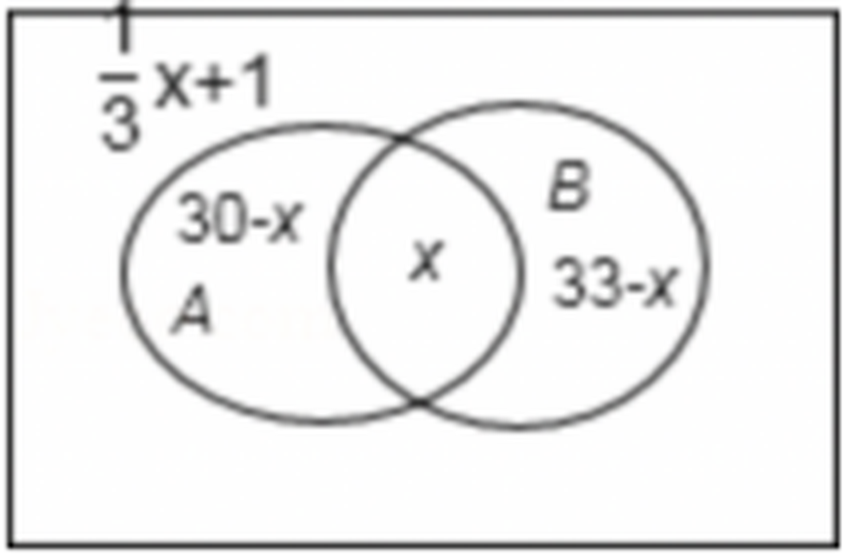
\includegraphics[width=0.30\textwidth]{figures/venn_AB_survey_50.png}
\end{center}

\ans{$21$}

\ifanswer
\solbegin
\step{由题意得赞成 $A$ 的人数 30，赞成 $B$ 的人数为 33，}
\step{设对 $A$、$B$ 都赞成的学生数为 $x$，则对 $A$、$B$ 都不赞成的学生数 $\dfrac{1}{3}x+1$，}
\step{如图得 $x+30-x+33-x+\dfrac{1}{3}x+1=50$，所以 $x=21$.}
\solend

\fi

\item 集合 $S=\{s\mid s=2n+1,n\in\Z\}$，$T=\{t\mid t=4n+1,n\in\Z\}$，则 $S$ \blankline[2.4em] $T$（填“$\subset$”“$\supset$”“$\subseteq$”或“$\supseteq$”）.

\ans{$S\supset T$}

\ifanswer
\solbegin
\step{对于 $S=\{s\mid s=2n+1,n\in\Z\}$ 为奇数，}
\step{而 $T=\{t\mid t=4n+1,n\in\Z\}$ 被 4 整除余 1 的奇数，所以 $S\supset T$.}
\solend

\fi

\item 已知集合 $A=\{x\mid -2<x<4\}$，$B=\{x\mid x^2-3ax+2a^2=0\}$，若 $A\cap B=B$，则实数 $a$ 的取值范围为 \blankline[4.4em].

\ans{$(-1,2)$}

\ifanswer
\solbegin
\step{因为 $A\cap B=B$，所以 $B\subseteq A$，}
\step{①当 $a=0$ 时，方程 $x^2-3ax+2a^2=0$ 的解为 $0$，$B\subseteq A$ 成立；}
\step{②当 $a\neq 0$ 时，方程 $x^2-3ax+2a^2=0$ 的解为 $2a$、$a$，}
\step{则 $-2<2a<4$ 且 $-2<a<4$，解得 $-1<a<2$ 且 $a\neq 0$；}
\step{综上所述，实数 $a$ 的取值范围为 $(-1,2)$.}
\solend

\fi

\item 当一个非空数集 $F$ 满足条件“若 $a$、$b\in F$，则 $a+b$、$a-b$、$ab\in F$，且当 $b\neq 0$ 时，$\dfrac{a}{b}\in F$”时，称 $F$ 为一个数域，以下四个关于数域的命题：

（1）$0$ 是任何数域的元素；（2）若数域 $F$ 有非零元素，则 $2026\in F$；

（3）集合 $P=\{x\mid x=3k,k\in\Z\}$ 为数域；（4）有理数集为数域；

其中，真命题的编号为 \blankline[4.4em]（写出所有真命题的编号）.

\ans{（1）（2）（4）}

\item 对于集合 $M$，定义函数 $f_M(x)=\begin{cases}-1,&x\in M\\ 1,&x\notin M\end{cases}$，对于两个集合 $M$、$N$，定义集合
$M\triangle N=\{x\mid f_M(x)\cdot f_N(x)=-1\}$，已知 $A=\{2,4,6,8,10\},B=\{1,2,4,8,16\}$，用 $|M|$ 表示有限集合 $M$ 中的元素个数，则对于任意集合 $M$，$|M\triangle A|+|M\triangle B|$ 的最小值为 \blankline[2.4em].

% 注：上面分段函数的第二行，原卷印作「1, $x\in M$」（两行都印 $x\in M$），与函数的定义矛盾，
%     本稿按文意订正为 $x\notin M$.
\ans{$4$}

\ifanswer
\solbegin
% 注：下面一行原卷印作「即 $M\triangle N\in\{x\mid x\in M\cup N\}$ 且 $x\in M\cap N$」，「$\in$」当为
%     「$=$」之误，且由 $f_M(x)f_N(x)=-1$ 应对应 $x\notin M\cap N$，本稿一并按文意订正.
\step{由 $M\triangle N$ 的定义得 $f_M(x)\cdot f_N(x)=-1$，}
\step{即 $M\triangle N=\{x\mid x\in M\cup N\text{ 且 }x\notin M\cap N\}$，}
\step{$|M\triangle A|+|M\triangle B|$ 要取得最小值，需满足 $A\cap B\subseteq M\subseteq A\cup B$，}
\step{此时 $|M\triangle A|+|M\triangle B|$ 的最小值为 $4$.}
\solend

\fi

\end{enumerate}

\bigsec{二、选择题}

\begin{enumerate}
\setcounter{enumi}{12}

\item 已知集合 $A=\{x\mid x=3m,m\in\N\}$，$B=\{x\mid x=3m+1,m\in\N\}$，$C=\{x\mid x=3m+2,m\in\N\}$，若 $a\in A$，$b\in B$，$c\in C$，则下列结论中可能成立的是\mbox{（\quad）}

\keepwithprev
A. $2021=a+b+c$\qquad B. $2021=abc$\qquad C. $2021=a+bc$\qquad D. $2021=a(b+c)$

\ans{C}

\ifanswer
\solbegin
\step{由题意设 $a=3m$，$b=3p+1$，$c=3n+2$，$m$、$p$、$n\in\N$，}
\step{则 $a+b+c=3m+3p+1+3n+2=3(m+p+n+1)$，}
\step{故 2021 不是 3 的整数倍，则 A 不可能；}
\step{$abc=3m(3p+1)(3n+2)$，同理 B 不可能；}
\step{$a+bc=3m+(3p+1)(3n+2)=3(m+3pn+2p+n)+2$，$2021=3\times 673+2$，}
\step{如取 $p=n=1$，则 $m=667$，即 $2021=3\times 667+4\times 5$，故 C 成立；}
\step{$a(b+c)=3m(3p+1+3n+2)=9m(p+n+1)$，同 A 可得 D 不可能.}
\step{故选 C.}
\solend

\fi

\item 设 $a$、$b$、$c$ 是实数，$x=a^2-2b+\dfrac{\pi}{3}$，$y=b^2-2c+\dfrac{\pi}{6}$，$z=c^2-2a+\dfrac{\pi}{2}$，则 $x$、$y$、$z$ 中至少有一个值\mbox{（\quad）}

\keepwithprev
A. 大于 $0$\qquad B. 等于 $0$\qquad C. 不大于 $0$\qquad D. 小于 $0$

\ans{A}

\ifanswer
\solbegin
\step{因为 $x+y+z=a^2-2b+\dfrac{\pi}{3}+b^2-2c+\dfrac{\pi}{6}+c^2-2a+\dfrac{\pi}{2}=(a-1)^2+(b-1)^2+(c-1)^2+\pi-3>0$，}
\step{假设 $x$、$y$、$z$ 都不大于 $0$，即 $x\leqslant 0$，$y\leqslant 0$，$z\leqslant 0$，}
\step{由同向不等式的可加性得 $x+y+z\leqslant 0$①，又 $x+y+z>0$ 与①式矛盾.}
\step{所以假设不成立，即原命题的结论 $x$、$y$、$z$ 中至少有一个大于 $0$. 故选 A.}
\solend

\fi

\item 命题“存在一个无理数，它的平方是有理数”的否定是\mbox{（\quad）}

\keepwithprev
A. 任意一个有理数，它的平方是有理数

B. 任意一个无理数，它的平方不是有理数

C. 存在一个有理数，它的平方是有理数

D. 存在一个无理数，它的平方不是有理数

\ans{B}

\ifanswer
\solbegin
\step{否定是任意一个无理数，它的平方不是有理数，故选 B.}
\solend

\fi

\item 设集合 $P_1=\{x\mid x^2+ax+1>0\}$，$P_2=\{x\mid x^2+ax+2>0\}$，$Q_1=\{x\mid x^2+x+b>0\}$，$Q_2=\{x\mid x^2+2x+b>0\}$，其中 $a$、$b\in\R$，下列说法正确的是\mbox{（\quad）}

\keepwithprev
A. 对任意 $a$，$P_1$ 是 $P_2$ 的子集，对任意 $b$，$Q_1$ 不是 $Q_2$ 的子集

B. 对任意 $a$，$P_1$ 是 $P_2$ 的子集，存在 $b$，使得 $Q_1$ 是 $Q_2$ 的子集

C. 对任意 $a$，使得 $P_1$ 不是 $P_2$ 的子集，对任意 $b$，$Q_1$ 不是 $Q_2$ 的子集

D. 对任意 $a$，使得 $P_1$ 不是 $P_2$ 的子集，存在 $b$，使得 $Q_1$ 不是 $Q_2$ 的子集

\ans{B}

\ifanswer
\solbegin
\step{对于集合 $P_1=\{x\mid x^2+ax+1>0\}$，$P_2=\{x\mid x^2+ax+2>0\}$，}
\step{得当 $m\in P_1$，即 $m^2+am+1>0$，得 $m^2+am+2>0$，}
\step{即有 $m\in P_2$，得对任意 $a$，$P_1$ 是 $P_2$ 的子集；}
\step{当 $b=5$ 时，$Q_1=\{x\mid x^2+x+5>0\}=\R$，$Q_2=\{x\mid x^2+2x+5>0\}=\R$，}
\step{得 $Q_1$ 是 $Q_2$ 的子集，故 A 错误，B 正确；}
\step{当 $b=1$ 时，$Q_1=\{x\mid x^2+x+1>0\}=\R$，}
\step{$Q_2=\{x\mid x^2+2x+1>0\}=\{x\mid x\neq -1\text{ 且 }x\in\R\}$，得 $Q_1$ 不是 $Q_2$ 的子集.}
\step{综上，对任意 $a$，$P_1$ 是 $P_2$ 的子集，存在 $b$，使得 $Q_1$ 是 $Q_2$ 的子集，}
\step{故 C 错误，D 错误.}
\step{故选 B.}
\solend

\fi

\end{enumerate}

\bigsec{三、解答题}

\begin{enumerate}
\setcounter{enumi}{16}

\item 已知集合 $A=\{x\mid 0<x-a\leqslant 5\}$，$B=\left\{x\mid -\dfrac{a}{2}<x\leqslant 6\right\}$.

\begin{enumerate}[label=(\arabic*)]
\item 若 $A\subseteq B$，求 $a$ 的取值范围.
\item 集合 $A$ 与 $B$ 能否相等？若能，求出 $a$ 的值，若不能，请说明理由.
\end{enumerate}

\ans{（1）$0\leqslant a\leqslant 1$；（2）不能，$a\in\varnothing$}

\ifanswer
\solbegin
\stepm{（1）}{由于 $A\subseteq B$，所以 $a+5\leqslant 6$，且 $-\dfrac{a}{2}\leqslant a$，解得 $0\leqslant a\leqslant 1$；}
\stepm{（2）}{$A=B$ 时，$a+5=6$，$-\dfrac{a}{2}=a$，解得 $a\in\varnothing$.}
\solend

\fi

\ansspace[6]

\item 已知 $\alpha:2x+m<0$，$\beta:-1<x<3$.

\begin{enumerate}[label=(\arabic*)]
\item 是否存在实数 $m$，使得 $\alpha$ 是 $\beta$ 的充分条件？若存在，求出实数 $m$ 的取值范围；
\item 是否存在实数 $m$，使得 $\alpha$ 是 $\beta$ 的必要条件？若存在，求出实数 $m$ 的取值范围.
\end{enumerate}

\ans{（1）不存在；（2）存在，$m\leqslant -6$}

\ansspace[6]

\item 已知 $\triangle ABC$ 的三边长分别为 $a,b,c$，证明：

\begin{enumerate}[label=(\arabic*)]
\item “$A=90^\circ$”是“关于 $x$ 的方程 $x^2+2ax+b^2=0$ 与 $x^2+2cx-b^2=0$ 有公共实根”的充分条件；
\item “$a=c$”是“关于 $x$ 的方程 $x^2+2ax+b^2=0$ 与 $x^2+2cx-b^2=0$ 没有公共实根”的充分非必要条件.
\end{enumerate}

\ans{（1）略；（2）略}

\ansspace[8]

\item 已知集合 $A$ 包含有 $n(n\in\N^*)$ 个元素，$A^+=\{x+y\mid x\text{、}y\in A\}$.

\begin{enumerate}[label=(\arabic*)]
\item 若 $A=\{0,1,2\}$，写出 $A^+$；
\item % 注：原卷此处印作「写出一个 $A^+$，使得 $A=A^+$」——$A$ 未给定，该问无法作答，
      %     与下方【解析】「取 $A=\{0\}$」不符，本稿按文意订正为「写出一个 $A$」.
      写出一个 $A$，使得 $A=A^+$；
\item 当 $n=4$ 时，是否存在集合 $A$，使得 $A^+=\{2,3,5,6,7,8,10\}$？若存在，求出此时的集合 $A$，若不存在，请说明理由.
\end{enumerate}

\ans{（1）$\{0,1,2,3,4\}$；（2）$A=\{0\}$；（3）不存在}

\ifanswer
\solbegin
\stepm{（1）}{由题意得 $0+0=0$，$0+1=1$，$0+2=2$，$1+1=2$，$1+2=3$，$2+2=4$ 都是 $A^+$ 中的元素，故 $A^+=\{0,1,2,3,4\}$；}
\stepm{（2）}{取 $A=\{0\}$，此时 $A^+=\{x+y\mid x\text{、}y\in A\}=\{0\}$，符合 $A=A^+$；}
\stepm{（3）}{当 $n=4$ 时，不存在集合 $A$，使得 $A^+=\{2,3,5,6,7,8,10\}$，理由如下：}
\step{假设存在 $A=\{a,b,c,d\}$，且 $a<b<c<d$，}
\step{则 $2a<a+b<a+c<b+c<b+d<c+d<2d$，}
\step{故 $2a,a+b,a+c,b+c,b+d,c+d,2d$ 为 $A^+$ 中 7 个不同的元素，}
\step{则 $2a=2$，$a+b=3$，$a+c=5$，$b+c=6$，$b+d=7$，$c+d=8$，$2d=10$，}
\step{解得 $a=1$，$b=2$，$c=4$，$d=5$，}
\step{此时 $c+d=9\in A^+$ 与 $9\notin A^+$ 矛盾，故假设不成立，}
\step{即不存在这样的集合 $A$.}
\solend

\fi

\ansspace[8]

% 压轴题：在其 \item 前先量一下版面，本页剩余高度不足 7cm 就另起一页。
\ansneed{7cm}

\item 已知集合 $A$ 为非空数集，对于集合 $A$，对 $A$ 中任意两个不同元素相加得到的和取绝对值，将这些绝对值重新组成一个新的集合，对于这一过程，我们定义为“自相加”，重新组成的集合叫做“集合 $A$ 的 1 次自相加集合”，再进行 $n-1$ 次“自相加”操作，组成的集合叫做“集合 $A$ 的 $n$ 次自相加集合”. 若集合 $A$ 的任意 $k$ 次自相加集合都不相等，则称集合 $A$ 为“完美自相加集合”，同理，我们可以定义出“$A$ 的 1 次自相减集合”，集合 $A$ 的 1 次自相加集合和 1 次自相减集合分别可表示为：$A^+=\{x\mid x=|a+b|,\ a\text{、}b\in A\}$，$A^-=\{x\mid x=|a-b|,\ a\text{、}b\in A\}$.

\begin{enumerate}[label=(\arabic*)]
\item 已知有两个集合，集合 $B=\{1,2,3,4\}$，集合 $C=\{k\mid k=2n+1,n\in\Z\}$，判断集合 $B$ 和集合 $C$ 是否是完美自相加集合，并说明理由；
\item 对（1）中的集合 $B$ 进行 11 次自相加操作后，求：集合 $B$ 的 11 次自相加集合的元素个数；
\item 若 $0\leqslant n\leqslant 2025$ 且 $n\in\N$，集合 $A=\{x\mid n\leqslant x\leqslant 2025,x\in\N\}$，$A^+\cap A^-=\varnothing$，求：$n$ 的最小值.
\end{enumerate}

\ans{（1）$B$ 是完美自相加集合，$C$ 不是完美自相加集合；（2）$2051$；（3）$675$}

\ifanswer
\solbegin
\stepm{（1）}{$B$ 是完美自相加集合，$C$ 不是完美自相加集合，}
\step{理由如下：因为集合 $B=\{1,2,3,4\}$，所以 $B^+=\{3,4,5,6,7\}$，}
\step{由此可得集合自相加后，}
\step{新的集合中最小的元素为自相加之前的集合中的最小两个元素之和，}
\step{所以显然集合 $B=\{1,2,3,4\}$ 的最小两个元素为 $1$，$2$，}
\step{所以 $B^+$ 中的最小元素为 $1+2=3$，}
\step{同理，2 次自相加后得到的集合中的最小元素是 $3+4=7$.}
\step{依照这样的规律，对集合 $B=\{1,2,3,4\}$ 进行任意次自相加操作后，}
\step{最小值总在变大，故不可能有相等集合，所以 $B$ 是完美自相加集合；}
\step{因为集合 $C=\{k\mid k=2n+1,n\in\Z\}$ 表示所有奇数构成的集合，}
\step{任何两个奇数相加的和都是偶数，}
\step{所以 $C^+=\{k\mid k=2n,n\in\Z\}$ 为所有偶数构成集合；}
\step{所以对 $C^+=\{k\mid k=2n,n\in\Z\}$ 再进行一次自相加操作，}
\step{因为任意两个偶数相加的和还是偶数，}
\step{所以后面集合不管进行多少次相加都与 $C^+=\{k\mid k=2n,n\in\Z\}$ 相同；}
\step{故 $C$ 不是完美自相加集合.}
\stepm{（2）}{由自相加性质得，对于集合 $B=\{1,2,3,4\}$，进行一次自相加，}
\step{得到集合的最小值必然是原来集合的两个最小元素值之和，}
\step{得到的最大值必然为原来集合的两个最大元素值之和，}
\step{且中间必然是连续的整数元素；}
\step{所以对集合 $B=\{1,2,3,4\}$ 进行 1 次自相加之后，}
\step{得到的集合最小两个元素为 $3$，$4$，最大的两个元素为 $6$，$7$；}
\step{进行第 2 次自相加，得到的集合最小两个元素为 $7$，$8$，}
\step{最大的两个元素为 $12$，$13$；}
\step{进行第 3 次自相加，得到的集合最小两个元素为 $15$，$16$，}
\step{最大的两个元素为 $24$，$25$；}
\step{进行第 4 次自相加，得到的集合最小两个元素为 $31$，$32$，}
\step{最大的两个元素为 $48$，$49$；}
\step{进行第 5 次自相加，得到的集合最小两个元素为 $63$，$64$，}
\step{最大的两个元素为 $96$，$97$；}
\step{进行第 6 次自相加，得到的集合最小两个元素为 $127$，$128$，}
\step{最大的两个元素为 $192$，$193$；}
\step{进行第 7 次自相加，得到的集合最小两个元素为 $255$，$256$，}
\step{最大的两个元素为 $384$，$385$；}
\step{进行第 8 次自相加，得到的集合最小两个元素为 $511$，$512$，}
\step{最大的两个元素为 $768$，$769$；}
\step{进行第 9 次自相加，得到的集合最小两个元素为 $1023$，$1024$，}
\step{最大的两个元素为 $1536$，$1537$；}
\step{进行第 10 次自相加，得到的集合最小两个元素为 $2047$，$2048$，}
\step{最大的两个元素为 $3072$，$3073$；}
\step{进行第 11 次自相加，得到的集合最小两个元素为 $4095$，$4096$，}
\step{最大的两个元素为 $6144$，$6145$；}
\step{因为集合 $B$ 的 $n$ 次自相加集合中的元素都是连续的整数，}
\step{所以集合 $B$ 进行 11 次自相加操作后的元素个数为 $6145-4095+1=2051$.}
\stepm{（3）}{因为 $0\leqslant n\leqslant 2025$ 且 $n\in\N$，集合 $A=\{x\mid n\leqslant x\leqslant 2025,x\in\N\}$，}
\step{所以 $A^+=\{x\mid 2n+1\leqslant x\leqslant 4049,x\in\N\}$，}
\step{$A^-=\{x\mid 1\leqslant x\leqslant 2025-n,x\in\N\}$，}
\step{要使 $A^+\cap A^-=\varnothing$，须使 $2n+1>2025-n$，所以 $n>\dfrac{2024}{3}=674\dfrac{2}{3}$，}
\step{又 $n\in\N$，故 $n$ 的最小值为 $675$.}
\solend

\fi

% 压轴题：其后已无内容，故作答区全用可丢弃胶水（\ansspace*）。
\ansspace*[12]

\end{enumerate}

\end{document}
"
%
% 原始材料是微信公众号图文（公众号「魔都数学加油站」），正文为 10 张 PNG 页（1080×1527）。
% 原文本身就是一份**讲评版**——题目下方直接印出【答案】或【解析】，选择题的答案印在解析末句
% 「故选 X」里。试题文字、答案与解析均照原卷录入（订正处见下），卷面上的粉色斜水印
% 「魔都数学加油站」属水印，未录入。
%
% 与原卷的排版差异（均已在 README「说明」中交代）：
%   ① 原文自**第 3 题**起（第 1、2 题未在该文中发布），故本稿题号亦自 3 起；
%   ② 原卷本就印有「一、填空题」「二、选择题」「三、解答题」三节标题（分别在原图 00/02/04.png
%      上，逐页核对过），本稿照原卷分节，只把标题改排成全稿统一的「大节标题」样式；
%   ③ 原卷填空、选择的答案直接印在题目下方（选择题只在解析末句「故选 X」中给出），本稿统一改为
%      试卷版隐去、答案版以【答案】给出，选择题的括注一律改排「\mbox{（\quad）}」并把答案移到选项之后，
%      使两版彻底分离；
%   ④ 原卷的集合符号大小写混用：第 3 题题干的实数集印成**粗体** $\mathbf{R}$，第 16 题题干与
%      第 16 题解析的印成正体 $R$；自然数集 $N$、整数集 $Z$ 一律正体。本稿按全稿惯例统一写作
%      $\R$、$\N$、$\Z$；
%   ⑤ 原卷未印副标题，本稿按全稿惯例补出副标题「集合与常用逻辑用语」；
%   ⑥ 原卷解答题子问编号为「（1）（2）」，本稿用嵌套 enumerate 排成同一形态；原卷第 15 题的
%      D 选项因原页翻页被截到下一页首页，本稿自然连排；
%   ⑦ 原卷解答题未留作答空间（讲评稿通篇是答案），本稿逐题补出书写留白，仅试卷版显示；
%   ⑧ 第 21 题题干里 $A^+$、$A^-$ 的定义含绝对值号（原卷作 $\{x\mid x=|a+b|,\ a\text{、}b\in A\}$
%      与 $\{x\mid x=|a-b|,\ a\text{、}b\in A\}$），本稿照原卷录入；2026-09-15 回原图逐处放大复核
%      时发现曾漏抄两处绝对值号、并把分隔逗号误写成 $\mid$，已按原卷订正（见 README 专记）。
%
% 原卷笔误三处（均已放大到能看清字形后核对，本稿按文意订正，并在 README 中写明原委）：
%   ① 第 12 题题干的分段函数 $f_M(x)$ 原卷两行都印作「$x\in M$」（$-1$ 与 $1$ 都取在 $M$ 上），
%      与「函数」的定义直接矛盾（$M$ 上无法同时取两个值），按文意订正第二行为 $x\notin M$；
%   ② 第 12 题【解析】首行原卷印「即 $M\triangle N\in\{x\mid x\in M\cup N\}$ 且 $x\in M\cap N$」，
%      其中「$\in$」当为「$=$」之误；且由 $f_M(x)f_N(x)=-1$ 应对应 $x\notin M\cap N$（原卷印作
%      $x\in M\cap N$，与上一行刚写出的对称差的定义相矛盾），本稿一并订正；
%   ③ 第 20 题(2)原卷印「写出一个 $A^+$，使得 $A=A^+$」——$A$ 未给定，该问无法作答，与紧接的
%      【解析】「取 $A=\{0\}$，此时 $A^+=\{0\}$，符合 $A=A^+$」不符，本稿按文意订正为
%      「写出一个 $A$，使得 $A=A^+$」.
%
% 原卷存疑一处（无法确证原意，本稿照抄原卷、未改）：
%   ① 第 5 题 ④ 原卷题干印 $S=\{x\mid |x|\leqslant\sqrt{3},x\in N\}$（该字母与 ③ 中的 $Z$
%      字形明显不同，$Z$ 有上下两横，已放大比对确认），而【解析】印「因为 $S=\{-1,0,1\}$」——
%      按 $x\in N$ 应为 $S=\{0,1\}$（或 $\{1\}$），题干与解析的口径不一致；但无论取哪一口径，
%      ④ 都是 $M$ 的子集、本题结论（填④）不变，故题干与解析均照抄原卷，未改。

\documentclass[a4paper,11pt]{article}
\usepackage{common}

\begin{document}

\examtitlest{2026--2027 年七宝中学高一上周末作业 2}{集合与常用逻辑用语}

\bigsec{一、填空题}

\begin{enumerate}
\setcounter{enumi}{2}

\item 已知 $a,x\in\R$，则“$x\in\{-a,a\}$”是“$|x|=a$”的 \blankline[4.4em] 条件.

\ans{必要不充分}

\item 设全集为 $U$，$A\subseteq U$，$B\subseteq U$，则“$A\subset B$”是“$\overline{B}\subset\overline{A}$”的 \blankline[4.4em] 条件.

\ans{充要}

\item 已知集合 $M=\{x\mid -\sqrt{5}<x<\sqrt{3},x\in\Z\}$，则下列集合是集合 $M$ 的子集的是 \blankline[4.4em]（填序号）.

① $P=\{-3,0,1\}$；② $Q=\{-1,0,1,2\}$；③ $R=\{y\mid -\pi<y<-1,y\in\Z\}$；

④ $S=\{x\mid |x|\leqslant\sqrt{3},x\in\N\}$.

\ans{④}

\ifanswer
\solbegin
\step{由已知得集合 $M=\{-2,-1,0,1\}$，}
\step{所以由子集的定义得选项①错误，②错误，}
\step{因为 $R=\{-3,-2\}$，所以集合 $R$ 不表示集合 $M$ 的子集，③错误，}
\step{因为 $S=\{-1,0,1\}$，所以是集合 $M$ 的子集，故正确.}
\step{故是集合 $M$ 的子集的是④.}
\solend

\fi

\item 已知 $x\in\R$，用反证法证明命题“若 $x^2-7x+10<0$，则 $2<x<5$”时，应该假设 \blankline[5em].

\ans{$x\leqslant 2$ 或 $x\geqslant 5$}

\item 设 $a_1,b_1,c_1,a_2,b_2,c_2$ 均为非零实数，方程 $a_1x^2+b_1x+c_1=0$ 和 $a_2x^2+b_2x+c_2=0$ 的解集分别为 $M$ 和 $N$，那么“$\dfrac{a_1}{a_2}=\dfrac{b_1}{b_2}=\dfrac{c_1}{c_2}$”是“$M=N$”的 \blankline[4.4em] 条件.

（填“充分非必要”、“必要非充分”、“充要”、或“既非充分又非必要”）

\ans{充分非必要}

\ifanswer
\solbegin
\step{$\dfrac{a_1}{a_2}=\dfrac{b_1}{b_2}=\dfrac{c_1}{c_2}$ 能推出 $M=N$，}
\step{若 $M=N=\varnothing$ 推不出 $\dfrac{a_1}{a_2}=\dfrac{b_1}{b_2}=\dfrac{c_1}{c_2}$，}
\step{所以“$\dfrac{a_1}{a_2}=\dfrac{b_1}{b_2}=\dfrac{c_1}{c_2}$”是“$M=N$”的“充分非必要”条件.}
\solend

\fi

\item 向 50 名学生调查对 $A$、$B$ 两事件的态度，有如下结果赞成 $A$ 的人数是全体的五分之三，其余的不赞成，赞成 $B$ 的比赞成 $A$ 的多 3 人，其余的不赞成；另外，对 $A$、$B$ 都不赞成的学生数比对 $A$、$B$ 都赞成的学生数的三分之一多 1 人. 则对 $A$、$B$ 都赞成的学生有 \blankline[2.4em] 人.

\begin{center}
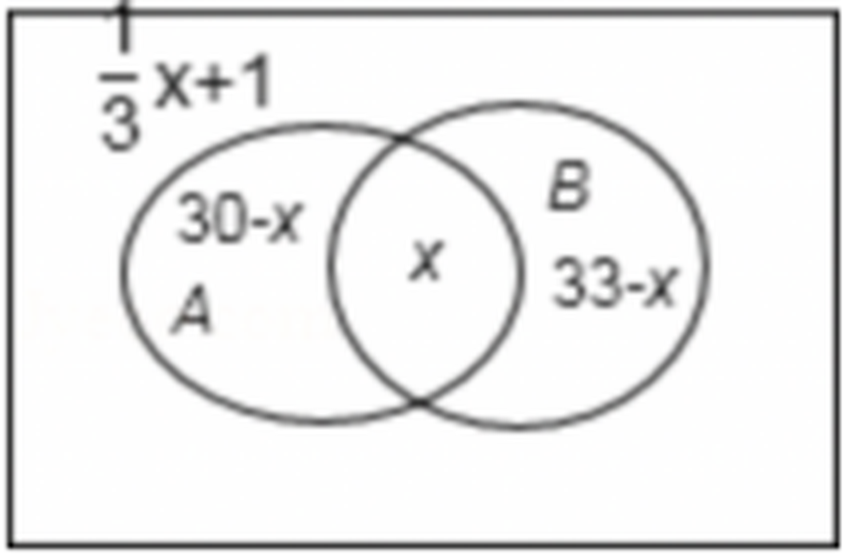
\includegraphics[width=0.30\textwidth]{figures/venn_AB_survey_50.png}
\end{center}

\ans{$21$}

\ifanswer
\solbegin
\step{由题意得赞成 $A$ 的人数 30，赞成 $B$ 的人数为 33，}
\step{设对 $A$、$B$ 都赞成的学生数为 $x$，则对 $A$、$B$ 都不赞成的学生数 $\dfrac{1}{3}x+1$，}
\step{如图得 $x+30-x+33-x+\dfrac{1}{3}x+1=50$，所以 $x=21$.}
\solend

\fi

\item 集合 $S=\{s\mid s=2n+1,n\in\Z\}$，$T=\{t\mid t=4n+1,n\in\Z\}$，则 $S$ \blankline[2.4em] $T$（填“$\subset$”“$\supset$”“$\subseteq$”或“$\supseteq$”）.

\ans{$S\supset T$}

\ifanswer
\solbegin
\step{对于 $S=\{s\mid s=2n+1,n\in\Z\}$ 为奇数，}
\step{而 $T=\{t\mid t=4n+1,n\in\Z\}$ 被 4 整除余 1 的奇数，所以 $S\supset T$.}
\solend

\fi

\item 已知集合 $A=\{x\mid -2<x<4\}$，$B=\{x\mid x^2-3ax+2a^2=0\}$，若 $A\cap B=B$，则实数 $a$ 的取值范围为 \blankline[4.4em].

\ans{$(-1,2)$}

\ifanswer
\solbegin
\step{因为 $A\cap B=B$，所以 $B\subseteq A$，}
\step{①当 $a=0$ 时，方程 $x^2-3ax+2a^2=0$ 的解为 $0$，$B\subseteq A$ 成立；}
\step{②当 $a\neq 0$ 时，方程 $x^2-3ax+2a^2=0$ 的解为 $2a$、$a$，}
\step{则 $-2<2a<4$ 且 $-2<a<4$，解得 $-1<a<2$ 且 $a\neq 0$；}
\step{综上所述，实数 $a$ 的取值范围为 $(-1,2)$.}
\solend

\fi

\item 当一个非空数集 $F$ 满足条件“若 $a$、$b\in F$，则 $a+b$、$a-b$、$ab\in F$，且当 $b\neq 0$ 时，$\dfrac{a}{b}\in F$”时，称 $F$ 为一个数域，以下四个关于数域的命题：

（1）$0$ 是任何数域的元素；（2）若数域 $F$ 有非零元素，则 $2026\in F$；

（3）集合 $P=\{x\mid x=3k,k\in\Z\}$ 为数域；（4）有理数集为数域；

其中，真命题的编号为 \blankline[4.4em]（写出所有真命题的编号）.

\ans{（1）（2）（4）}

\item 对于集合 $M$，定义函数 $f_M(x)=\begin{cases}-1,&x\in M\\ 1,&x\notin M\end{cases}$，对于两个集合 $M$、$N$，定义集合
$M\triangle N=\{x\mid f_M(x)\cdot f_N(x)=-1\}$，已知 $A=\{2,4,6,8,10\},B=\{1,2,4,8,16\}$，用 $|M|$ 表示有限集合 $M$ 中的元素个数，则对于任意集合 $M$，$|M\triangle A|+|M\triangle B|$ 的最小值为 \blankline[2.4em].

% 注：上面分段函数的第二行，原卷印作「1, $x\in M$」（两行都印 $x\in M$），与函数的定义矛盾，
%     本稿按文意订正为 $x\notin M$.
\ans{$4$}

\ifanswer
\solbegin
% 注：下面一行原卷印作「即 $M\triangle N\in\{x\mid x\in M\cup N\}$ 且 $x\in M\cap N$」，「$\in$」当为
%     「$=$」之误，且由 $f_M(x)f_N(x)=-1$ 应对应 $x\notin M\cap N$，本稿一并按文意订正.
\step{由 $M\triangle N$ 的定义得 $f_M(x)\cdot f_N(x)=-1$，}
\step{即 $M\triangle N=\{x\mid x\in M\cup N\text{ 且 }x\notin M\cap N\}$，}
\step{$|M\triangle A|+|M\triangle B|$ 要取得最小值，需满足 $A\cap B\subseteq M\subseteq A\cup B$，}
\step{此时 $|M\triangle A|+|M\triangle B|$ 的最小值为 $4$.}
\solend

\fi

\end{enumerate}

\bigsec{二、选择题}

\begin{enumerate}
\setcounter{enumi}{12}

\item 已知集合 $A=\{x\mid x=3m,m\in\N\}$，$B=\{x\mid x=3m+1,m\in\N\}$，$C=\{x\mid x=3m+2,m\in\N\}$，若 $a\in A$，$b\in B$，$c\in C$，则下列结论中可能成立的是\mbox{（\quad）}

\keepwithprev
A. $2021=a+b+c$\qquad B. $2021=abc$\qquad C. $2021=a+bc$\qquad D. $2021=a(b+c)$

\ans{C}

\ifanswer
\solbegin
\step{由题意设 $a=3m$，$b=3p+1$，$c=3n+2$，$m$、$p$、$n\in\N$，}
\step{则 $a+b+c=3m+3p+1+3n+2=3(m+p+n+1)$，}
\step{故 2021 不是 3 的整数倍，则 A 不可能；}
\step{$abc=3m(3p+1)(3n+2)$，同理 B 不可能；}
\step{$a+bc=3m+(3p+1)(3n+2)=3(m+3pn+2p+n)+2$，$2021=3\times 673+2$，}
\step{如取 $p=n=1$，则 $m=667$，即 $2021=3\times 667+4\times 5$，故 C 成立；}
\step{$a(b+c)=3m(3p+1+3n+2)=9m(p+n+1)$，同 A 可得 D 不可能.}
\step{故选 C.}
\solend

\fi

\item 设 $a$、$b$、$c$ 是实数，$x=a^2-2b+\dfrac{\pi}{3}$，$y=b^2-2c+\dfrac{\pi}{6}$，$z=c^2-2a+\dfrac{\pi}{2}$，则 $x$、$y$、$z$ 中至少有一个值\mbox{（\quad）}

\keepwithprev
A. 大于 $0$\qquad B. 等于 $0$\qquad C. 不大于 $0$\qquad D. 小于 $0$

\ans{A}

\ifanswer
\solbegin
\step{因为 $x+y+z=a^2-2b+\dfrac{\pi}{3}+b^2-2c+\dfrac{\pi}{6}+c^2-2a+\dfrac{\pi}{2}=(a-1)^2+(b-1)^2+(c-1)^2+\pi-3>0$，}
\step{假设 $x$、$y$、$z$ 都不大于 $0$，即 $x\leqslant 0$，$y\leqslant 0$，$z\leqslant 0$，}
\step{由同向不等式的可加性得 $x+y+z\leqslant 0$①，又 $x+y+z>0$ 与①式矛盾.}
\step{所以假设不成立，即原命题的结论 $x$、$y$、$z$ 中至少有一个大于 $0$. 故选 A.}
\solend

\fi

\item 命题“存在一个无理数，它的平方是有理数”的否定是\mbox{（\quad）}

\keepwithprev
A. 任意一个有理数，它的平方是有理数

B. 任意一个无理数，它的平方不是有理数

C. 存在一个有理数，它的平方是有理数

D. 存在一个无理数，它的平方不是有理数

\ans{B}

\ifanswer
\solbegin
\step{否定是任意一个无理数，它的平方不是有理数，故选 B.}
\solend

\fi

\item 设集合 $P_1=\{x\mid x^2+ax+1>0\}$，$P_2=\{x\mid x^2+ax+2>0\}$，$Q_1=\{x\mid x^2+x+b>0\}$，$Q_2=\{x\mid x^2+2x+b>0\}$，其中 $a$、$b\in\R$，下列说法正确的是\mbox{（\quad）}

\keepwithprev
A. 对任意 $a$，$P_1$ 是 $P_2$ 的子集，对任意 $b$，$Q_1$ 不是 $Q_2$ 的子集

B. 对任意 $a$，$P_1$ 是 $P_2$ 的子集，存在 $b$，使得 $Q_1$ 是 $Q_2$ 的子集

C. 对任意 $a$，使得 $P_1$ 不是 $P_2$ 的子集，对任意 $b$，$Q_1$ 不是 $Q_2$ 的子集

D. 对任意 $a$，使得 $P_1$ 不是 $P_2$ 的子集，存在 $b$，使得 $Q_1$ 不是 $Q_2$ 的子集

\ans{B}

\ifanswer
\solbegin
\step{对于集合 $P_1=\{x\mid x^2+ax+1>0\}$，$P_2=\{x\mid x^2+ax+2>0\}$，}
\step{得当 $m\in P_1$，即 $m^2+am+1>0$，得 $m^2+am+2>0$，}
\step{即有 $m\in P_2$，得对任意 $a$，$P_1$ 是 $P_2$ 的子集；}
\step{当 $b=5$ 时，$Q_1=\{x\mid x^2+x+5>0\}=\R$，$Q_2=\{x\mid x^2+2x+5>0\}=\R$，}
\step{得 $Q_1$ 是 $Q_2$ 的子集，故 A 错误，B 正确；}
\step{当 $b=1$ 时，$Q_1=\{x\mid x^2+x+1>0\}=\R$，}
\step{$Q_2=\{x\mid x^2+2x+1>0\}=\{x\mid x\neq -1\text{ 且 }x\in\R\}$，得 $Q_1$ 不是 $Q_2$ 的子集.}
\step{综上，对任意 $a$，$P_1$ 是 $P_2$ 的子集，存在 $b$，使得 $Q_1$ 是 $Q_2$ 的子集，}
\step{故 C 错误，D 错误.}
\step{故选 B.}
\solend

\fi

\end{enumerate}

\bigsec{三、解答题}

\begin{enumerate}
\setcounter{enumi}{16}

\item 已知集合 $A=\{x\mid 0<x-a\leqslant 5\}$，$B=\left\{x\mid -\dfrac{a}{2}<x\leqslant 6\right\}$.

\begin{enumerate}[label=(\arabic*)]
\item 若 $A\subseteq B$，求 $a$ 的取值范围.
\item 集合 $A$ 与 $B$ 能否相等？若能，求出 $a$ 的值，若不能，请说明理由.
\end{enumerate}

\ans{（1）$0\leqslant a\leqslant 1$；（2）不能，$a\in\varnothing$}

\ifanswer
\solbegin
\stepm{（1）}{由于 $A\subseteq B$，所以 $a+5\leqslant 6$，且 $-\dfrac{a}{2}\leqslant a$，解得 $0\leqslant a\leqslant 1$；}
\stepm{（2）}{$A=B$ 时，$a+5=6$，$-\dfrac{a}{2}=a$，解得 $a\in\varnothing$.}
\solend

\fi

\ansspace[6]

\item 已知 $\alpha:2x+m<0$，$\beta:-1<x<3$.

\begin{enumerate}[label=(\arabic*)]
\item 是否存在实数 $m$，使得 $\alpha$ 是 $\beta$ 的充分条件？若存在，求出实数 $m$ 的取值范围；
\item 是否存在实数 $m$，使得 $\alpha$ 是 $\beta$ 的必要条件？若存在，求出实数 $m$ 的取值范围.
\end{enumerate}

\ans{（1）不存在；（2）存在，$m\leqslant -6$}

\ansspace[6]

\item 已知 $\triangle ABC$ 的三边长分别为 $a,b,c$，证明：

\begin{enumerate}[label=(\arabic*)]
\item “$A=90^\circ$”是“关于 $x$ 的方程 $x^2+2ax+b^2=0$ 与 $x^2+2cx-b^2=0$ 有公共实根”的充分条件；
\item “$a=c$”是“关于 $x$ 的方程 $x^2+2ax+b^2=0$ 与 $x^2+2cx-b^2=0$ 没有公共实根”的充分非必要条件.
\end{enumerate}

\ans{（1）略；（2）略}

\ansspace[8]

\item 已知集合 $A$ 包含有 $n(n\in\N^*)$ 个元素，$A^+=\{x+y\mid x\text{、}y\in A\}$.

\begin{enumerate}[label=(\arabic*)]
\item 若 $A=\{0,1,2\}$，写出 $A^+$；
\item % 注：原卷此处印作「写出一个 $A^+$，使得 $A=A^+$」——$A$ 未给定，该问无法作答，
      %     与下方【解析】「取 $A=\{0\}$」不符，本稿按文意订正为「写出一个 $A$」.
      写出一个 $A$，使得 $A=A^+$；
\item 当 $n=4$ 时，是否存在集合 $A$，使得 $A^+=\{2,3,5,6,7,8,10\}$？若存在，求出此时的集合 $A$，若不存在，请说明理由.
\end{enumerate}

\ans{（1）$\{0,1,2,3,4\}$；（2）$A=\{0\}$；（3）不存在}

\ifanswer
\solbegin
\stepm{（1）}{由题意得 $0+0=0$，$0+1=1$，$0+2=2$，$1+1=2$，$1+2=3$，$2+2=4$ 都是 $A^+$ 中的元素，故 $A^+=\{0,1,2,3,4\}$；}
\stepm{（2）}{取 $A=\{0\}$，此时 $A^+=\{x+y\mid x\text{、}y\in A\}=\{0\}$，符合 $A=A^+$；}
\stepm{（3）}{当 $n=4$ 时，不存在集合 $A$，使得 $A^+=\{2,3,5,6,7,8,10\}$，理由如下：}
\step{假设存在 $A=\{a,b,c,d\}$，且 $a<b<c<d$，}
\step{则 $2a<a+b<a+c<b+c<b+d<c+d<2d$，}
\step{故 $2a,a+b,a+c,b+c,b+d,c+d,2d$ 为 $A^+$ 中 7 个不同的元素，}
\step{则 $2a=2$，$a+b=3$，$a+c=5$，$b+c=6$，$b+d=7$，$c+d=8$，$2d=10$，}
\step{解得 $a=1$，$b=2$，$c=4$，$d=5$，}
\step{此时 $c+d=9\in A^+$ 与 $9\notin A^+$ 矛盾，故假设不成立，}
\step{即不存在这样的集合 $A$.}
\solend

\fi

\ansspace[8]

% 压轴题：在其 \item 前先量一下版面，本页剩余高度不足 7cm 就另起一页。
\ansneed{7cm}

\item 已知集合 $A$ 为非空数集，对于集合 $A$，对 $A$ 中任意两个不同元素相加得到的和取绝对值，将这些绝对值重新组成一个新的集合，对于这一过程，我们定义为“自相加”，重新组成的集合叫做“集合 $A$ 的 1 次自相加集合”，再进行 $n-1$ 次“自相加”操作，组成的集合叫做“集合 $A$ 的 $n$ 次自相加集合”. 若集合 $A$ 的任意 $k$ 次自相加集合都不相等，则称集合 $A$ 为“完美自相加集合”，同理，我们可以定义出“$A$ 的 1 次自相减集合”，集合 $A$ 的 1 次自相加集合和 1 次自相减集合分别可表示为：$A^+=\{x\mid x=|a+b|,\ a\text{、}b\in A\}$，$A^-=\{x\mid x=|a-b|,\ a\text{、}b\in A\}$.

\begin{enumerate}[label=(\arabic*)]
\item 已知有两个集合，集合 $B=\{1,2,3,4\}$，集合 $C=\{k\mid k=2n+1,n\in\Z\}$，判断集合 $B$ 和集合 $C$ 是否是完美自相加集合，并说明理由；
\item 对（1）中的集合 $B$ 进行 11 次自相加操作后，求：集合 $B$ 的 11 次自相加集合的元素个数；
\item 若 $0\leqslant n\leqslant 2025$ 且 $n\in\N$，集合 $A=\{x\mid n\leqslant x\leqslant 2025,x\in\N\}$，$A^+\cap A^-=\varnothing$，求：$n$ 的最小值.
\end{enumerate}

\ans{（1）$B$ 是完美自相加集合，$C$ 不是完美自相加集合；（2）$2051$；（3）$675$}

\ifanswer
\solbegin
\stepm{（1）}{$B$ 是完美自相加集合，$C$ 不是完美自相加集合，}
\step{理由如下：因为集合 $B=\{1,2,3,4\}$，所以 $B^+=\{3,4,5,6,7\}$，}
\step{由此可得集合自相加后，}
\step{新的集合中最小的元素为自相加之前的集合中的最小两个元素之和，}
\step{所以显然集合 $B=\{1,2,3,4\}$ 的最小两个元素为 $1$，$2$，}
\step{所以 $B^+$ 中的最小元素为 $1+2=3$，}
\step{同理，2 次自相加后得到的集合中的最小元素是 $3+4=7$.}
\step{依照这样的规律，对集合 $B=\{1,2,3,4\}$ 进行任意次自相加操作后，}
\step{最小值总在变大，故不可能有相等集合，所以 $B$ 是完美自相加集合；}
\step{因为集合 $C=\{k\mid k=2n+1,n\in\Z\}$ 表示所有奇数构成的集合，}
\step{任何两个奇数相加的和都是偶数，}
\step{所以 $C^+=\{k\mid k=2n,n\in\Z\}$ 为所有偶数构成集合；}
\step{所以对 $C^+=\{k\mid k=2n,n\in\Z\}$ 再进行一次自相加操作，}
\step{因为任意两个偶数相加的和还是偶数，}
\step{所以后面集合不管进行多少次相加都与 $C^+=\{k\mid k=2n,n\in\Z\}$ 相同；}
\step{故 $C$ 不是完美自相加集合.}
\stepm{（2）}{由自相加性质得，对于集合 $B=\{1,2,3,4\}$，进行一次自相加，}
\step{得到集合的最小值必然是原来集合的两个最小元素值之和，}
\step{得到的最大值必然为原来集合的两个最大元素值之和，}
\step{且中间必然是连续的整数元素；}
\step{所以对集合 $B=\{1,2,3,4\}$ 进行 1 次自相加之后，}
\step{得到的集合最小两个元素为 $3$，$4$，最大的两个元素为 $6$，$7$；}
\step{进行第 2 次自相加，得到的集合最小两个元素为 $7$，$8$，}
\step{最大的两个元素为 $12$，$13$；}
\step{进行第 3 次自相加，得到的集合最小两个元素为 $15$，$16$，}
\step{最大的两个元素为 $24$，$25$；}
\step{进行第 4 次自相加，得到的集合最小两个元素为 $31$，$32$，}
\step{最大的两个元素为 $48$，$49$；}
\step{进行第 5 次自相加，得到的集合最小两个元素为 $63$，$64$，}
\step{最大的两个元素为 $96$，$97$；}
\step{进行第 6 次自相加，得到的集合最小两个元素为 $127$，$128$，}
\step{最大的两个元素为 $192$，$193$；}
\step{进行第 7 次自相加，得到的集合最小两个元素为 $255$，$256$，}
\step{最大的两个元素为 $384$，$385$；}
\step{进行第 8 次自相加，得到的集合最小两个元素为 $511$，$512$，}
\step{最大的两个元素为 $768$，$769$；}
\step{进行第 9 次自相加，得到的集合最小两个元素为 $1023$，$1024$，}
\step{最大的两个元素为 $1536$，$1537$；}
\step{进行第 10 次自相加，得到的集合最小两个元素为 $2047$，$2048$，}
\step{最大的两个元素为 $3072$，$3073$；}
\step{进行第 11 次自相加，得到的集合最小两个元素为 $4095$，$4096$，}
\step{最大的两个元素为 $6144$，$6145$；}
\step{因为集合 $B$ 的 $n$ 次自相加集合中的元素都是连续的整数，}
\step{所以集合 $B$ 进行 11 次自相加操作后的元素个数为 $6145-4095+1=2051$.}
\stepm{（3）}{因为 $0\leqslant n\leqslant 2025$ 且 $n\in\N$，集合 $A=\{x\mid n\leqslant x\leqslant 2025,x\in\N\}$，}
\step{所以 $A^+=\{x\mid 2n+1\leqslant x\leqslant 4049,x\in\N\}$，}
\step{$A^-=\{x\mid 1\leqslant x\leqslant 2025-n,x\in\N\}$，}
\step{要使 $A^+\cap A^-=\varnothing$，须使 $2n+1>2025-n$，所以 $n>\dfrac{2024}{3}=674\dfrac{2}{3}$，}
\step{又 $n\in\N$，故 $n$ 的最小值为 $675$.}
\solend

\fi

% 压轴题：其后已无内容，故作答区全用可丢弃胶水（\ansspace*）。
\ansspace*[12]

\end{enumerate}

\end{document}
"
%
% 原始材料是微信公众号图文（公众号「魔都数学加油站」），正文为 10 张 PNG 页（1080×1527）。
% 原文本身就是一份**讲评版**——题目下方直接印出【答案】或【解析】，选择题的答案印在解析末句
% 「故选 X」里。试题文字、答案与解析均照原卷录入（订正处见下），卷面上的粉色斜水印
% 「魔都数学加油站」属水印，未录入。
%
% 与原卷的排版差异（均已在 README「说明」中交代）：
%   ① 原文自**第 3 题**起（第 1、2 题未在该文中发布），故本稿题号亦自 3 起；
%   ② 原卷本就印有「一、填空题」「二、选择题」「三、解答题」三节标题（分别在原图 00/02/04.png
%      上，逐页核对过），本稿照原卷分节，只把标题改排成全稿统一的「大节标题」样式；
%   ③ 原卷填空、选择的答案直接印在题目下方（选择题只在解析末句「故选 X」中给出），本稿统一改为
%      试卷版隐去、答案版以【答案】给出，选择题的括注一律改排「\mbox{（\quad）}」并把答案移到选项之后，
%      使两版彻底分离；
%   ④ 原卷的集合符号大小写混用：第 3 题题干的实数集印成**粗体** $\mathbf{R}$，第 16 题题干与
%      第 16 题解析的印成正体 $R$；自然数集 $N$、整数集 $Z$ 一律正体。本稿按全稿惯例统一写作
%      $\R$、$\N$、$\Z$；
%   ⑤ 原卷未印副标题，本稿按全稿惯例补出副标题「集合与常用逻辑用语」；
%   ⑥ 原卷解答题子问编号为「（1）（2）」，本稿用嵌套 enumerate 排成同一形态；原卷第 15 题的
%      D 选项因原页翻页被截到下一页首页，本稿自然连排；
%   ⑦ 原卷解答题未留作答空间（讲评稿通篇是答案），本稿逐题补出书写留白，仅试卷版显示；
%   ⑧ 第 21 题题干里 $A^+$、$A^-$ 的定义含绝对值号（原卷作 $\{x\mid x=|a+b|,\ a\text{、}b\in A\}$
%      与 $\{x\mid x=|a-b|,\ a\text{、}b\in A\}$），本稿照原卷录入；2026-09-15 回原图逐处放大复核
%      时发现曾漏抄两处绝对值号、并把分隔逗号误写成 $\mid$，已按原卷订正（见 README 专记）。
%
% 原卷笔误三处（均已放大到能看清字形后核对，本稿按文意订正，并在 README 中写明原委）：
%   ① 第 12 题题干的分段函数 $f_M(x)$ 原卷两行都印作「$x\in M$」（$-1$ 与 $1$ 都取在 $M$ 上），
%      与「函数」的定义直接矛盾（$M$ 上无法同时取两个值），按文意订正第二行为 $x\notin M$；
%   ② 第 12 题【解析】首行原卷印「即 $M\triangle N\in\{x\mid x\in M\cup N\}$ 且 $x\in M\cap N$」，
%      其中「$\in$」当为「$=$」之误；且由 $f_M(x)f_N(x)=-1$ 应对应 $x\notin M\cap N$（原卷印作
%      $x\in M\cap N$，与上一行刚写出的对称差的定义相矛盾），本稿一并订正；
%   ③ 第 20 题(2)原卷印「写出一个 $A^+$，使得 $A=A^+$」——$A$ 未给定，该问无法作答，与紧接的
%      【解析】「取 $A=\{0\}$，此时 $A^+=\{0\}$，符合 $A=A^+$」不符，本稿按文意订正为
%      「写出一个 $A$，使得 $A=A^+$」.
%
% 原卷存疑一处（无法确证原意，本稿照抄原卷、未改）：
%   ① 第 5 题 ④ 原卷题干印 $S=\{x\mid |x|\leqslant\sqrt{3},x\in N\}$（该字母与 ③ 中的 $Z$
%      字形明显不同，$Z$ 有上下两横，已放大比对确认），而【解析】印「因为 $S=\{-1,0,1\}$」——
%      按 $x\in N$ 应为 $S=\{0,1\}$（或 $\{1\}$），题干与解析的口径不一致；但无论取哪一口径，
%      ④ 都是 $M$ 的子集、本题结论（填④）不变，故题干与解析均照抄原卷，未改。

\documentclass[a4paper,11pt]{article}
\usepackage{common}

\begin{document}

\examtitlest{2026--2027 年七宝中学高一上周末作业 2}{集合与常用逻辑用语}

\bigsec{一、填空题}

\begin{enumerate}
\setcounter{enumi}{2}

\item 已知 $a,x\in\R$，则“$x\in\{-a,a\}$”是“$|x|=a$”的 \blankline[4.4em] 条件.

\ans{必要不充分}

\item 设全集为 $U$，$A\subseteq U$，$B\subseteq U$，则“$A\subset B$”是“$\overline{B}\subset\overline{A}$”的 \blankline[4.4em] 条件.

\ans{充要}

\item 已知集合 $M=\{x\mid -\sqrt{5}<x<\sqrt{3},x\in\Z\}$，则下列集合是集合 $M$ 的子集的是 \blankline[4.4em]（填序号）.

① $P=\{-3,0,1\}$；② $Q=\{-1,0,1,2\}$；③ $R=\{y\mid -\pi<y<-1,y\in\Z\}$；

④ $S=\{x\mid |x|\leqslant\sqrt{3},x\in\N\}$.

\ans{④}

\ifanswer
\solbegin
\step{由已知得集合 $M=\{-2,-1,0,1\}$，}
\step{所以由子集的定义得选项①错误，②错误，}
\step{因为 $R=\{-3,-2\}$，所以集合 $R$ 不表示集合 $M$ 的子集，③错误，}
\step{因为 $S=\{-1,0,1\}$，所以是集合 $M$ 的子集，故正确.}
\step{故是集合 $M$ 的子集的是④.}
\solend

\fi

\item 已知 $x\in\R$，用反证法证明命题“若 $x^2-7x+10<0$，则 $2<x<5$”时，应该假设 \blankline[5em].

\ans{$x\leqslant 2$ 或 $x\geqslant 5$}

\item 设 $a_1,b_1,c_1,a_2,b_2,c_2$ 均为非零实数，方程 $a_1x^2+b_1x+c_1=0$ 和 $a_2x^2+b_2x+c_2=0$ 的解集分别为 $M$ 和 $N$，那么“$\dfrac{a_1}{a_2}=\dfrac{b_1}{b_2}=\dfrac{c_1}{c_2}$”是“$M=N$”的 \blankline[4.4em] 条件.

（填“充分非必要”、“必要非充分”、“充要”、或“既非充分又非必要”）

\ans{充分非必要}

\ifanswer
\solbegin
\step{$\dfrac{a_1}{a_2}=\dfrac{b_1}{b_2}=\dfrac{c_1}{c_2}$ 能推出 $M=N$，}
\step{若 $M=N=\varnothing$ 推不出 $\dfrac{a_1}{a_2}=\dfrac{b_1}{b_2}=\dfrac{c_1}{c_2}$，}
\step{所以“$\dfrac{a_1}{a_2}=\dfrac{b_1}{b_2}=\dfrac{c_1}{c_2}$”是“$M=N$”的“充分非必要”条件.}
\solend

\fi

\item 向 50 名学生调查对 $A$、$B$ 两事件的态度，有如下结果赞成 $A$ 的人数是全体的五分之三，其余的不赞成，赞成 $B$ 的比赞成 $A$ 的多 3 人，其余的不赞成；另外，对 $A$、$B$ 都不赞成的学生数比对 $A$、$B$ 都赞成的学生数的三分之一多 1 人. 则对 $A$、$B$ 都赞成的学生有 \blankline[2.4em] 人.

\begin{center}
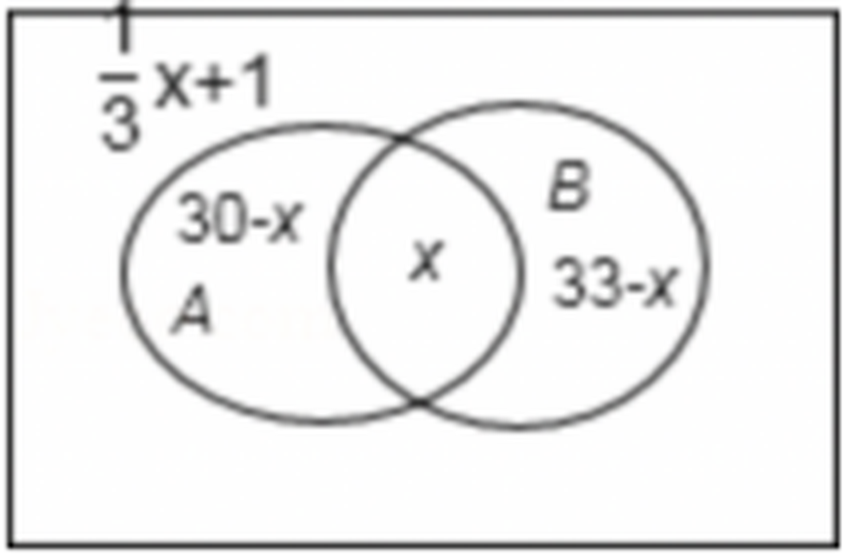
\includegraphics[width=0.30\textwidth]{figures/venn_AB_survey_50.png}
\end{center}

\ans{$21$}

\ifanswer
\solbegin
\step{由题意得赞成 $A$ 的人数 30，赞成 $B$ 的人数为 33，}
\step{设对 $A$、$B$ 都赞成的学生数为 $x$，则对 $A$、$B$ 都不赞成的学生数 $\dfrac{1}{3}x+1$，}
\step{如图得 $x+30-x+33-x+\dfrac{1}{3}x+1=50$，所以 $x=21$.}
\solend

\fi

\item 集合 $S=\{s\mid s=2n+1,n\in\Z\}$，$T=\{t\mid t=4n+1,n\in\Z\}$，则 $S$ \blankline[2.4em] $T$（填“$\subset$”“$\supset$”“$\subseteq$”或“$\supseteq$”）.

\ans{$S\supset T$}

\ifanswer
\solbegin
\step{对于 $S=\{s\mid s=2n+1,n\in\Z\}$ 为奇数，}
\step{而 $T=\{t\mid t=4n+1,n\in\Z\}$ 被 4 整除余 1 的奇数，所以 $S\supset T$.}
\solend

\fi

\item 已知集合 $A=\{x\mid -2<x<4\}$，$B=\{x\mid x^2-3ax+2a^2=0\}$，若 $A\cap B=B$，则实数 $a$ 的取值范围为 \blankline[4.4em].

\ans{$(-1,2)$}

\ifanswer
\solbegin
\step{因为 $A\cap B=B$，所以 $B\subseteq A$，}
\step{①当 $a=0$ 时，方程 $x^2-3ax+2a^2=0$ 的解为 $0$，$B\subseteq A$ 成立；}
\step{②当 $a\neq 0$ 时，方程 $x^2-3ax+2a^2=0$ 的解为 $2a$、$a$，}
\step{则 $-2<2a<4$ 且 $-2<a<4$，解得 $-1<a<2$ 且 $a\neq 0$；}
\step{综上所述，实数 $a$ 的取值范围为 $(-1,2)$.}
\solend

\fi

\item 当一个非空数集 $F$ 满足条件“若 $a$、$b\in F$，则 $a+b$、$a-b$、$ab\in F$，且当 $b\neq 0$ 时，$\dfrac{a}{b}\in F$”时，称 $F$ 为一个数域，以下四个关于数域的命题：

（1）$0$ 是任何数域的元素；（2）若数域 $F$ 有非零元素，则 $2026\in F$；

（3）集合 $P=\{x\mid x=3k,k\in\Z\}$ 为数域；（4）有理数集为数域；

其中，真命题的编号为 \blankline[4.4em]（写出所有真命题的编号）.

\ans{（1）（2）（4）}

\item 对于集合 $M$，定义函数 $f_M(x)=\begin{cases}-1,&x\in M\\ 1,&x\notin M\end{cases}$，对于两个集合 $M$、$N$，定义集合
$M\triangle N=\{x\mid f_M(x)\cdot f_N(x)=-1\}$，已知 $A=\{2,4,6,8,10\},B=\{1,2,4,8,16\}$，用 $|M|$ 表示有限集合 $M$ 中的元素个数，则对于任意集合 $M$，$|M\triangle A|+|M\triangle B|$ 的最小值为 \blankline[2.4em].

% 注：上面分段函数的第二行，原卷印作「1, $x\in M$」（两行都印 $x\in M$），与函数的定义矛盾，
%     本稿按文意订正为 $x\notin M$.
\ans{$4$}

\ifanswer
\solbegin
% 注：下面一行原卷印作「即 $M\triangle N\in\{x\mid x\in M\cup N\}$ 且 $x\in M\cap N$」，「$\in$」当为
%     「$=$」之误，且由 $f_M(x)f_N(x)=-1$ 应对应 $x\notin M\cap N$，本稿一并按文意订正.
\step{由 $M\triangle N$ 的定义得 $f_M(x)\cdot f_N(x)=-1$，}
\step{即 $M\triangle N=\{x\mid x\in M\cup N\text{ 且 }x\notin M\cap N\}$，}
\step{$|M\triangle A|+|M\triangle B|$ 要取得最小值，需满足 $A\cap B\subseteq M\subseteq A\cup B$，}
\step{此时 $|M\triangle A|+|M\triangle B|$ 的最小值为 $4$.}
\solend

\fi

\end{enumerate}

\bigsec{二、选择题}

\begin{enumerate}
\setcounter{enumi}{12}

\item 已知集合 $A=\{x\mid x=3m,m\in\N\}$，$B=\{x\mid x=3m+1,m\in\N\}$，$C=\{x\mid x=3m+2,m\in\N\}$，若 $a\in A$，$b\in B$，$c\in C$，则下列结论中可能成立的是\mbox{（\quad）}

\keepwithprev
A. $2021=a+b+c$\qquad B. $2021=abc$\qquad C. $2021=a+bc$\qquad D. $2021=a(b+c)$

\ans{C}

\ifanswer
\solbegin
\step{由题意设 $a=3m$，$b=3p+1$，$c=3n+2$，$m$、$p$、$n\in\N$，}
\step{则 $a+b+c=3m+3p+1+3n+2=3(m+p+n+1)$，}
\step{故 2021 不是 3 的整数倍，则 A 不可能；}
\step{$abc=3m(3p+1)(3n+2)$，同理 B 不可能；}
\step{$a+bc=3m+(3p+1)(3n+2)=3(m+3pn+2p+n)+2$，$2021=3\times 673+2$，}
\step{如取 $p=n=1$，则 $m=667$，即 $2021=3\times 667+4\times 5$，故 C 成立；}
\step{$a(b+c)=3m(3p+1+3n+2)=9m(p+n+1)$，同 A 可得 D 不可能.}
\step{故选 C.}
\solend

\fi

\item 设 $a$、$b$、$c$ 是实数，$x=a^2-2b+\dfrac{\pi}{3}$，$y=b^2-2c+\dfrac{\pi}{6}$，$z=c^2-2a+\dfrac{\pi}{2}$，则 $x$、$y$、$z$ 中至少有一个值\mbox{（\quad）}

\keepwithprev
A. 大于 $0$\qquad B. 等于 $0$\qquad C. 不大于 $0$\qquad D. 小于 $0$

\ans{A}

\ifanswer
\solbegin
\step{因为 $x+y+z=a^2-2b+\dfrac{\pi}{3}+b^2-2c+\dfrac{\pi}{6}+c^2-2a+\dfrac{\pi}{2}=(a-1)^2+(b-1)^2+(c-1)^2+\pi-3>0$，}
\step{假设 $x$、$y$、$z$ 都不大于 $0$，即 $x\leqslant 0$，$y\leqslant 0$，$z\leqslant 0$，}
\step{由同向不等式的可加性得 $x+y+z\leqslant 0$①，又 $x+y+z>0$ 与①式矛盾.}
\step{所以假设不成立，即原命题的结论 $x$、$y$、$z$ 中至少有一个大于 $0$. 故选 A.}
\solend

\fi

\item 命题“存在一个无理数，它的平方是有理数”的否定是\mbox{（\quad）}

\keepwithprev
A. 任意一个有理数，它的平方是有理数

B. 任意一个无理数，它的平方不是有理数

C. 存在一个有理数，它的平方是有理数

D. 存在一个无理数，它的平方不是有理数

\ans{B}

\ifanswer
\solbegin
\step{否定是任意一个无理数，它的平方不是有理数，故选 B.}
\solend

\fi

\item 设集合 $P_1=\{x\mid x^2+ax+1>0\}$，$P_2=\{x\mid x^2+ax+2>0\}$，$Q_1=\{x\mid x^2+x+b>0\}$，$Q_2=\{x\mid x^2+2x+b>0\}$，其中 $a$、$b\in\R$，下列说法正确的是\mbox{（\quad）}

\keepwithprev
A. 对任意 $a$，$P_1$ 是 $P_2$ 的子集，对任意 $b$，$Q_1$ 不是 $Q_2$ 的子集

B. 对任意 $a$，$P_1$ 是 $P_2$ 的子集，存在 $b$，使得 $Q_1$ 是 $Q_2$ 的子集

C. 对任意 $a$，使得 $P_1$ 不是 $P_2$ 的子集，对任意 $b$，$Q_1$ 不是 $Q_2$ 的子集

D. 对任意 $a$，使得 $P_1$ 不是 $P_2$ 的子集，存在 $b$，使得 $Q_1$ 不是 $Q_2$ 的子集

\ans{B}

\ifanswer
\solbegin
\step{对于集合 $P_1=\{x\mid x^2+ax+1>0\}$，$P_2=\{x\mid x^2+ax+2>0\}$，}
\step{得当 $m\in P_1$，即 $m^2+am+1>0$，得 $m^2+am+2>0$，}
\step{即有 $m\in P_2$，得对任意 $a$，$P_1$ 是 $P_2$ 的子集；}
\step{当 $b=5$ 时，$Q_1=\{x\mid x^2+x+5>0\}=\R$，$Q_2=\{x\mid x^2+2x+5>0\}=\R$，}
\step{得 $Q_1$ 是 $Q_2$ 的子集，故 A 错误，B 正确；}
\step{当 $b=1$ 时，$Q_1=\{x\mid x^2+x+1>0\}=\R$，}
\step{$Q_2=\{x\mid x^2+2x+1>0\}=\{x\mid x\neq -1\text{ 且 }x\in\R\}$，得 $Q_1$ 不是 $Q_2$ 的子集.}
\step{综上，对任意 $a$，$P_1$ 是 $P_2$ 的子集，存在 $b$，使得 $Q_1$ 是 $Q_2$ 的子集，}
\step{故 C 错误，D 错误.}
\step{故选 B.}
\solend

\fi

\end{enumerate}

\bigsec{三、解答题}

\begin{enumerate}
\setcounter{enumi}{16}

\item 已知集合 $A=\{x\mid 0<x-a\leqslant 5\}$，$B=\left\{x\mid -\dfrac{a}{2}<x\leqslant 6\right\}$.

\begin{enumerate}[label=(\arabic*)]
\item 若 $A\subseteq B$，求 $a$ 的取值范围.
\item 集合 $A$ 与 $B$ 能否相等？若能，求出 $a$ 的值，若不能，请说明理由.
\end{enumerate}

\ans{（1）$0\leqslant a\leqslant 1$；（2）不能，$a\in\varnothing$}

\ifanswer
\solbegin
\stepm{（1）}{由于 $A\subseteq B$，所以 $a+5\leqslant 6$，且 $-\dfrac{a}{2}\leqslant a$，解得 $0\leqslant a\leqslant 1$；}
\stepm{（2）}{$A=B$ 时，$a+5=6$，$-\dfrac{a}{2}=a$，解得 $a\in\varnothing$.}
\solend

\fi

\ansspace[6]

\item 已知 $\alpha:2x+m<0$，$\beta:-1<x<3$.

\begin{enumerate}[label=(\arabic*)]
\item 是否存在实数 $m$，使得 $\alpha$ 是 $\beta$ 的充分条件？若存在，求出实数 $m$ 的取值范围；
\item 是否存在实数 $m$，使得 $\alpha$ 是 $\beta$ 的必要条件？若存在，求出实数 $m$ 的取值范围.
\end{enumerate}

\ans{（1）不存在；（2）存在，$m\leqslant -6$}

\ansspace[6]

\item 已知 $\triangle ABC$ 的三边长分别为 $a,b,c$，证明：

\begin{enumerate}[label=(\arabic*)]
\item “$A=90^\circ$”是“关于 $x$ 的方程 $x^2+2ax+b^2=0$ 与 $x^2+2cx-b^2=0$ 有公共实根”的充分条件；
\item “$a=c$”是“关于 $x$ 的方程 $x^2+2ax+b^2=0$ 与 $x^2+2cx-b^2=0$ 没有公共实根”的充分非必要条件.
\end{enumerate}

\ans{（1）略；（2）略}

\ansspace[8]

\item 已知集合 $A$ 包含有 $n(n\in\N^*)$ 个元素，$A^+=\{x+y\mid x\text{、}y\in A\}$.

\begin{enumerate}[label=(\arabic*)]
\item 若 $A=\{0,1,2\}$，写出 $A^+$；
\item % 注：原卷此处印作「写出一个 $A^+$，使得 $A=A^+$」——$A$ 未给定，该问无法作答，
      %     与下方【解析】「取 $A=\{0\}$」不符，本稿按文意订正为「写出一个 $A$」.
      写出一个 $A$，使得 $A=A^+$；
\item 当 $n=4$ 时，是否存在集合 $A$，使得 $A^+=\{2,3,5,6,7,8,10\}$？若存在，求出此时的集合 $A$，若不存在，请说明理由.
\end{enumerate}

\ans{（1）$\{0,1,2,3,4\}$；（2）$A=\{0\}$；（3）不存在}

\ifanswer
\solbegin
\stepm{（1）}{由题意得 $0+0=0$，$0+1=1$，$0+2=2$，$1+1=2$，$1+2=3$，$2+2=4$ 都是 $A^+$ 中的元素，故 $A^+=\{0,1,2,3,4\}$；}
\stepm{（2）}{取 $A=\{0\}$，此时 $A^+=\{x+y\mid x\text{、}y\in A\}=\{0\}$，符合 $A=A^+$；}
\stepm{（3）}{当 $n=4$ 时，不存在集合 $A$，使得 $A^+=\{2,3,5,6,7,8,10\}$，理由如下：}
\step{假设存在 $A=\{a,b,c,d\}$，且 $a<b<c<d$，}
\step{则 $2a<a+b<a+c<b+c<b+d<c+d<2d$，}
\step{故 $2a,a+b,a+c,b+c,b+d,c+d,2d$ 为 $A^+$ 中 7 个不同的元素，}
\step{则 $2a=2$，$a+b=3$，$a+c=5$，$b+c=6$，$b+d=7$，$c+d=8$，$2d=10$，}
\step{解得 $a=1$，$b=2$，$c=4$，$d=5$，}
\step{此时 $c+d=9\in A^+$ 与 $9\notin A^+$ 矛盾，故假设不成立，}
\step{即不存在这样的集合 $A$.}
\solend

\fi

\ansspace[8]

% 压轴题：在其 \item 前先量一下版面，本页剩余高度不足 7cm 就另起一页。
\ansneed{7cm}

\item 已知集合 $A$ 为非空数集，对于集合 $A$，对 $A$ 中任意两个不同元素相加得到的和取绝对值，将这些绝对值重新组成一个新的集合，对于这一过程，我们定义为“自相加”，重新组成的集合叫做“集合 $A$ 的 1 次自相加集合”，再进行 $n-1$ 次“自相加”操作，组成的集合叫做“集合 $A$ 的 $n$ 次自相加集合”. 若集合 $A$ 的任意 $k$ 次自相加集合都不相等，则称集合 $A$ 为“完美自相加集合”，同理，我们可以定义出“$A$ 的 1 次自相减集合”，集合 $A$ 的 1 次自相加集合和 1 次自相减集合分别可表示为：$A^+=\{x\mid x=|a+b|,\ a\text{、}b\in A\}$，$A^-=\{x\mid x=|a-b|,\ a\text{、}b\in A\}$.

\begin{enumerate}[label=(\arabic*)]
\item 已知有两个集合，集合 $B=\{1,2,3,4\}$，集合 $C=\{k\mid k=2n+1,n\in\Z\}$，判断集合 $B$ 和集合 $C$ 是否是完美自相加集合，并说明理由；
\item 对（1）中的集合 $B$ 进行 11 次自相加操作后，求：集合 $B$ 的 11 次自相加集合的元素个数；
\item 若 $0\leqslant n\leqslant 2025$ 且 $n\in\N$，集合 $A=\{x\mid n\leqslant x\leqslant 2025,x\in\N\}$，$A^+\cap A^-=\varnothing$，求：$n$ 的最小值.
\end{enumerate}

\ans{（1）$B$ 是完美自相加集合，$C$ 不是完美自相加集合；（2）$2051$；（3）$675$}

\ifanswer
\solbegin
\stepm{（1）}{$B$ 是完美自相加集合，$C$ 不是完美自相加集合，}
\step{理由如下：因为集合 $B=\{1,2,3,4\}$，所以 $B^+=\{3,4,5,6,7\}$，}
\step{由此可得集合自相加后，}
\step{新的集合中最小的元素为自相加之前的集合中的最小两个元素之和，}
\step{所以显然集合 $B=\{1,2,3,4\}$ 的最小两个元素为 $1$，$2$，}
\step{所以 $B^+$ 中的最小元素为 $1+2=3$，}
\step{同理，2 次自相加后得到的集合中的最小元素是 $3+4=7$.}
\step{依照这样的规律，对集合 $B=\{1,2,3,4\}$ 进行任意次自相加操作后，}
\step{最小值总在变大，故不可能有相等集合，所以 $B$ 是完美自相加集合；}
\step{因为集合 $C=\{k\mid k=2n+1,n\in\Z\}$ 表示所有奇数构成的集合，}
\step{任何两个奇数相加的和都是偶数，}
\step{所以 $C^+=\{k\mid k=2n,n\in\Z\}$ 为所有偶数构成集合；}
\step{所以对 $C^+=\{k\mid k=2n,n\in\Z\}$ 再进行一次自相加操作，}
\step{因为任意两个偶数相加的和还是偶数，}
\step{所以后面集合不管进行多少次相加都与 $C^+=\{k\mid k=2n,n\in\Z\}$ 相同；}
\step{故 $C$ 不是完美自相加集合.}
\stepm{（2）}{由自相加性质得，对于集合 $B=\{1,2,3,4\}$，进行一次自相加，}
\step{得到集合的最小值必然是原来集合的两个最小元素值之和，}
\step{得到的最大值必然为原来集合的两个最大元素值之和，}
\step{且中间必然是连续的整数元素；}
\step{所以对集合 $B=\{1,2,3,4\}$ 进行 1 次自相加之后，}
\step{得到的集合最小两个元素为 $3$，$4$，最大的两个元素为 $6$，$7$；}
\step{进行第 2 次自相加，得到的集合最小两个元素为 $7$，$8$，}
\step{最大的两个元素为 $12$，$13$；}
\step{进行第 3 次自相加，得到的集合最小两个元素为 $15$，$16$，}
\step{最大的两个元素为 $24$，$25$；}
\step{进行第 4 次自相加，得到的集合最小两个元素为 $31$，$32$，}
\step{最大的两个元素为 $48$，$49$；}
\step{进行第 5 次自相加，得到的集合最小两个元素为 $63$，$64$，}
\step{最大的两个元素为 $96$，$97$；}
\step{进行第 6 次自相加，得到的集合最小两个元素为 $127$，$128$，}
\step{最大的两个元素为 $192$，$193$；}
\step{进行第 7 次自相加，得到的集合最小两个元素为 $255$，$256$，}
\step{最大的两个元素为 $384$，$385$；}
\step{进行第 8 次自相加，得到的集合最小两个元素为 $511$，$512$，}
\step{最大的两个元素为 $768$，$769$；}
\step{进行第 9 次自相加，得到的集合最小两个元素为 $1023$，$1024$，}
\step{最大的两个元素为 $1536$，$1537$；}
\step{进行第 10 次自相加，得到的集合最小两个元素为 $2047$，$2048$，}
\step{最大的两个元素为 $3072$，$3073$；}
\step{进行第 11 次自相加，得到的集合最小两个元素为 $4095$，$4096$，}
\step{最大的两个元素为 $6144$，$6145$；}
\step{因为集合 $B$ 的 $n$ 次自相加集合中的元素都是连续的整数，}
\step{所以集合 $B$ 进行 11 次自相加操作后的元素个数为 $6145-4095+1=2051$.}
\stepm{（3）}{因为 $0\leqslant n\leqslant 2025$ 且 $n\in\N$，集合 $A=\{x\mid n\leqslant x\leqslant 2025,x\in\N\}$，}
\step{所以 $A^+=\{x\mid 2n+1\leqslant x\leqslant 4049,x\in\N\}$，}
\step{$A^-=\{x\mid 1\leqslant x\leqslant 2025-n,x\in\N\}$，}
\step{要使 $A^+\cap A^-=\varnothing$，须使 $2n+1>2025-n$，所以 $n>\dfrac{2024}{3}=674\dfrac{2}{3}$，}
\step{又 $n\in\N$，故 $n$ 的最小值为 $675$.}
\solend

\fi

% 压轴题：其后已无内容，故作答区全用可丢弃胶水（\ansspace*）。
\ansspace*[12]

\end{enumerate}

\end{document}
